

 \documentclass[a4paper]{asimbook}

   \usepackage{a4wide}
   \usepackage{makeidx}
   \usepackage{fancyhdr}
   \usepackage{graphicx}
   \usepackage{multicol}
   \usepackage{float}
   \usepackage{textcomp}
   \usepackage{alltt}
   \usepackage{times}
   \ifx\pdfoutput\undefined
     \usepackage[ps2pdf,pagebackref=true,colorlinks=true,linkcolor=blue]{hyperref}
     \usepackage{pspicture}
   \else
     \usepackage[pdftex,pagebackref=true,colorlinks=true,linkcolor=blue]{hyperref}
   \fi
   \usepackage{doxygen}

   \makeindex
   \setcounter{tocdepth}{1}
   \renewcommand{\footrulewidth}{0.4pt}
   \raggedbottom


 \begin{document}

   \begin{titlepage}
     \vspace*{7cm}
     \begin{center}
     {\Large Kite - Detailed Router Reference Manual\\[1ex]\large 1.0 }\\
     \vspace*{1cm}
     {\large Generated by Doxygen 1.8.5}\\
     \vspace*{0.5cm}
     {\small Mon Oct 1 2018 14:29:11}\\
     \end{center}
   \end{titlepage}

   \clearemptydoublepage
   \pagenumbering{roman}

   \tableofcontents
   \clearemptydoublepage

   \pagenumbering{arabic}
\section{Detailed Router Documentation}
\label{index}\hypertarget{index}{}This documentation adresses two level of explanations \+:


\begin{DoxyItemize}
\item The {\bfseries A\+PI} description which explains how to use \mbox{\hyperlink{namespaceKite}{Kite}}, thoses parts as flagged as {\bfseries A\+PI}. 
\item The internal description which details how \mbox{\hyperlink{namespaceKite}{Kite}} do things. It\textquotesingle{}s mostly intended for myself to help me not to forget how I\textquotesingle{}ve done things when debug time will come... It may also be valuable to people who may want to use or patch \mbox{\hyperlink{namespaceKite}{Kite}} for their own purpose (my secret hope). 
\end{DoxyItemize}

Additionnal documents\+:
\begin{DoxyItemize}
\item \mbox{\hyperlink{group__grpSynthHierarchy}{Synthetic Hierarchy (A\+PI)}} 
\end{DoxyItemize}
\section{Notes}
\label{pageNotes}
\hypertarget{pageNotes}{}
\hypertarget{pageNotes_Summary}{}\subsection{Summary}\label{pageNotes_Summary}

\begin{DoxyItemize}
\item \hyperlink{pageNotes_ssecVariousNotes}{Various Things to Remeber}
\item \hyperlink{pageNotes_secPendingModifications}{Pending Modifications}
\item \hyperlink{pageNotes_secModificationsHistory}{Modifications History}
\item \hyperlink{pageNotes_ssecArchitectureChanges}{Changes in the general architecture}
\begin{DoxyItemize}
\item \hyperlink{pageNotes_ssecModificationsKiteEngine}{Changes in Kite\+Engine class design}
\item \hyperlink{pageNotes_ssecModificationsDataNegociate}{Changes in Data\+Negociate class design}
\item \hyperlink{pageNotes_ssecModificationsTrackElement}{Changes in Track\+Element class design}
\item \hyperlink{pageNotes_ssecModificationsTrackSegment}{Changes in Track\+Segment class design}
\item \hyperlink{pageNotes_ssecModificationsAutoSegment}{Changes in Auto\+Segment class design}
\item \hyperlink{pageNotes_ssecModificationsAutoContact}{Changes in Auto\+Contact class design}
\end{DoxyItemize}
\item \hyperlink{pageNotes_ssecBugBusting}{Bug Solving Memento}
\item \hyperlink{pageNotes_ssecNanoRoute}{Evaluation with Cadence Nano\+Route}
\end{DoxyItemize}\hypertarget{pageNotes_ssecVariousNotes}{}\subsection{Various Things to Remember}\label{pageNotes_ssecVariousNotes}

\begin{DoxyItemize}
\item {\bfseries Determinism checking.} The trace level to get only determinism related log is {\ttfamily 500}. Each line for the determinism is prepended with \textquotesingle{}Deter$\vert$\textquotesingle{}, possible with some leading spaces.
\item The router only sees/manages the aligned segment sets (through a pseudo-\/ decorator on their canonical segment). So the non-\/canonical segments and the contacts should not be handled at all at this level.
\item Do do confuse the Session\+::\+Event, events that modificate the state of the \hyperlink{namespaceKite}{Kite} database (insert, move or remove \hyperlink{classKite_1_1TrackSegment}{Track\+Segment} in \hyperlink{classKite_1_1Track}{Track}) and the \hyperlink{classKite_1_1RoutingEvent}{Routing\+Event} class which request that a segment must be processed.
\item In the various processing method of \hyperlink{classKite_1_1RoutingEvent}{Routing\+Event}, when a \hyperlink{classKite_1_1TrackSegment}{Track\+Segment} can be inserted inside a \hyperlink{classKite_1_1Track}{Track} a Session\+::\+Event is generated but no further \hyperlink{classKite_1_1RoutingEvent}{Routing\+Event}, this end the placement processus of segment (until it is ripped-\/up).
\item Auto\+Segment do not invalidate their S/T anchor contacts.
\item Auto\+Contact invalidate their anchored upon Auto\+Segment.
\item Now that the Hurricane database is deterministic, the router seems to be likewise.
\item {\bfseries Reduce/raise mechanism}. To manage {\itshape same layer} dogleg this mechanism has been implemented. When a candidate dogleg perpandicular segment length shrink below one pitch it is removed from any track to become {\itshape invisible}. Conversely, when a reduced segment length expand over one pitch generate a new \hyperlink{classKite_1_1RoutingEvent}{Routing\+Event} to insert it. All this is managed in the \hyperlink{classKite_1_1Session_a5bd93abe1416952ace15a98dbeeed124}{Session\+::revalidate()} method.
\end{DoxyItemize}\hypertarget{pageNotes_secPendingModifications}{}\subsection{Pending Modifications}\label{pageNotes_secPendingModifications}

\begin{DoxyItemize}
\item In \hyperlink{classKite_1_1SegmentAction_a324f17f0f5a09b76344eb2e003695d74}{Segment\+Action\+::do\+Action()}, completly disable the movement of \hyperlink{classKite_1_1TrackSegment}{Track\+Segment} on it\textquotesingle{}s target \hyperlink{classKite_1_1Track}{Track} axis. This should not be needed as, if the algorithm as worked correctly, the next time it\textquotesingle{}s \hyperlink{classKite_1_1RoutingEvent}{Routing\+Event} is processed, the target \hyperlink{classKite_1_1Track}{Track} will have a free space to insert into. Then the \hyperlink{classKite_1_1Track}{Track} insertion will set the \hyperlink{classKite_1_1TrackSegment}{Track\+Segment} axis.
\item Has to complete the lazy evaluation of the \hyperlink{classKite_1_1TrackSegment}{Track\+Segment} / \hyperlink{classKite_1_1DataNegociate}{Data\+Negociate} / \hyperlink{classKite_1_1RoutingEvent}{Routing\+Event}. There is still some redundancy when the key of the \hyperlink{classKite_1_1RoutingEvent}{Routing\+Event} is updated.
\item In \textbf{ Auto\+Contact\+::update\+Topology()} \& \textbf{ Auto\+Contact\+::update\+Geometry()} we could avoid to systematically run through the Hooks to cache the connected segments. This can be done once at the first call of either method (whichever comes first) on the first revalidate. Afterwards the cache can be updated only by \textbf{ Auto\+Contact\+::update\+Topology()}.
\item The canonization is done in two places, directly on a set of aligneds Auto\+Segments through \textbf{ Auto\+Segment\+::canonize()} and for the whole net Session\+::\+\_\+canonize(), which is called after the initial creation and each time the topology is modificated. The later may be suppressed if we uses more intelligently the former, and gain some more speedup.
\end{DoxyItemize}\hypertarget{pageNotes_secModificationsHistory}{}\subsection{Modifications History}\label{pageNotes_secModificationsHistory}
\hypertarget{pageNotes_ssecArchitectureChanges}{}\subsubsection{Changes in the general architecture}\label{pageNotes_ssecArchitectureChanges}

\begin{DoxyItemize}
\item {\bfseries Lazy Update.} Update of \hyperlink{classKite_1_1DataNegociate}{Data\+Negociate} and \hyperlink{classKite_1_1RoutingEvent}{Routing\+Event} are now delayed until the event is processed, and systematically done at this point. Thus, the explicit invalidation of those objects is no longer needed. The revalidation is no longer triggered by the revalidation of \hyperlink{classKite_1_1TrackSegment}{Track\+Segment}.
\end{DoxyItemize}\hypertarget{pageNotes_ssecModificationsKiteEngine}{}\subsubsection{Changes in Kite\+Engine class design}\label{pageNotes_ssecModificationsKiteEngine}

\begin{DoxyItemize}
\item Suppress the lookup table of \textbf{ Hurricane\+::\+Segment} toward \hyperlink{classKite_1_1TrackSegment}{Track\+Segment}. Instead uses the Observer mecanism between \textbf{ Katabatic\+::\+Auto\+Segment} and \hyperlink{classKite_1_1TrackSegment}{Track\+Segment}.
\end{DoxyItemize}\hypertarget{pageNotes_ssecModificationsDataNegociate}{}\subsubsection{Changes in Data\+Negociate class design}\label{pageNotes_ssecModificationsDataNegociate}

\begin{DoxyItemize}
\item Merge in the separate class {\ttfamily Cost}.
\item Suppress the {\ttfamily Slack\+State\+::\+Desalignate}, due to the simplificated structure of the Auto\+Segment/\+Auto\+Contacts (no more collapseds, or forced alignements).
\item Displace the computation and caching of the perpandiculars and perpandicular free interval from \hyperlink{classKite_1_1RoutingEvent}{Routing\+Event} into \hyperlink{classKite_1_1DataNegociate}{Data\+Negociate}. Allows code factorization with the attractors computation, and data size reduction as there is exaclty one \hyperlink{classKite_1_1DataNegociate}{Data\+Negociate} but there may be more than one \hyperlink{classKite_1_1RoutingEvent}{Routing\+Event} for the same \hyperlink{classKite_1_1TrackSegment}{Track\+Segment}.
\end{DoxyItemize}\hypertarget{pageNotes_ssecModificationsTrackElement}{}\subsubsection{Changes in Track\+Element class design}\label{pageNotes_ssecModificationsTrackElement}

\begin{DoxyItemize}
\item Due to the simplificated structure of the Katabatic contacts (terminal, turn, vtee \& htee), there\textquotesingle{}s no longer collapsed Auto\+Segment or {\itshape expandable} contacts. The {\bfseries desalignate} feature, relaxing constraints due to collapsed segments or contacts with more than three segments, is no longer implemented. {\bfseries Have to redevelop a method to break long segments linked} {\bfseries by H\+Tee or V\+Tee.}
\end{DoxyItemize}\hypertarget{pageNotes_ssecModificationsTrackSegment}{}\subsubsection{Changes in Track\+Segment class design}\label{pageNotes_ssecModificationsTrackSegment}

\begin{DoxyItemize}
\item The method {\ttfamily Track\+Segment\+::\+\_\+post\+Modify()} is merged with \hyperlink{classKite_1_1TrackSegment_a10a45c049d0bd7d01c7eff1c5441c7a2}{Track\+Segment\+::\+\_\+post\+Doglegs()} as, in the context of \hyperlink{classKite_1_1TrackSegment}{Track\+Segment} the only used topological modifications goes through the creation of one or more dogleg.
\end{DoxyItemize}\hypertarget{pageNotes_ssecModificationsAutoSegment}{}\subsubsection{Changes in Auto\+Segment class design}\label{pageNotes_ssecModificationsAutoSegment}

\begin{DoxyItemize}
\item In \textbf{ Auto\+Segment\+::\+\_\+make\+Dogleg()}, update the local/global status of the involved Auto\+Segment and re-\/canonize only what is necessary. Thus, guarantee that the net\textquotesingle{}s topology is still valid after this method call and no topological update is needed at \hyperlink{classKite_1_1Session}{Session} level (should be {\itshape much} faster). In this method, the code sharing between Auto\+Horizontal and Auto\+Vertical can still be increased (update mechanisms are identicals).
\item The {\ttfamily id} support is now also implemented at Hurricane level. We may choose to use as a replacement of the one already present in Auto\+Segment. But in that case, we at least must cache the id in the Auto\+Segment. So we will not gain in memory footprint, the only benefit would be to have coherent id number throughout all the tools, but the sequentiality will be lost (this may not be a big issue).
\end{DoxyItemize}\hypertarget{pageNotes_ssecModificationsAutoContact}{}\subsubsection{Changes in Auto\+Contact class design}\label{pageNotes_ssecModificationsAutoContact}

\begin{DoxyItemize}
\item In \textbf{ Auto\+Segment\+::invalidate()}, no longer uses collection to walk through attached Auto\+Segment, directly uses the cache. Much simple and efficient as we exactly know what is attached on every kind of contact.
\end{DoxyItemize}\hypertarget{pageNotes_ssecBugBusting}{}\subsection{Bug Solving Memento}\label{pageNotes_ssecBugBusting}
{\bfseries L\+UT lookup change\+:} When breaking a \hyperlink{classKite_1_1TrackSegment}{Track\+Segment}, the break may not occurs in the associated canonical Auto\+Segment. In that case the {\ttfamily dogleg\mbox{[}O\mbox{]}} will not match the one that is looked up for the broken (canonical) segment. Thus it was not a bug but a misunderstanding...

{\bfseries Overlap of perpandiculars after a dogleg creation\+:} The axis of the new parallel was not set to the axis of it\textquotesingle{}s parent. This was due to the uses of \textbf{ Auto\+Segment\+::set\+Axis()} in Auto\+Horizontal\+::\+\_\+make\+Dogleg() which silently do nothing on non-\/canonical Auto\+Segment, and at this point, the re-\/canonisation did not yet take place. Now Uses Auto\+Segment\+::\+\_\+set\+Axis() the atomic variant wich works inconditionnaly.\hypertarget{pageNotes_ssecNanoRoute}{}\subsection{Evaluation with Cadence Nano\+Route}\label{pageNotes_ssecNanoRoute}
To perform a comparison with Nano\+Route the procedure is as follow\+:


\begin{DoxyItemize}
\item Export the design in Alliance {\ttfamily D\+EF} format. It will generate both {\ttfamily D\+EF} file and the supporting {\ttfamily L\+EF} file containing the technology and the abstract of all the standard cell of the design. As Alliance uses symbolic units (lambda), they are translated with the simple rule\+: {\bfseries 1 lambda == 1 micron}.
\item Run the commands in Nano\+Route\+:
\begin{DoxyItemize}
\item {\ttfamily load\+Lef\+File design.\+lef}
\item {\ttfamily load\+Def\+File design.\+def}
\item {\ttfamily generate\+Tracks}
\item {\ttfamily generate\+Vias}
\item {\ttfamily set\+Nano\+Route\+Mode -\/quiet -\/droute\+Fix\+Antenna 0}
\item {\ttfamily set\+Nano\+Route\+Mode -\/quiet -\/droute\+Start\+Iteration default}
\item {\ttfamily set\+Nano\+Route\+Mode -\/quiet -\/route\+Top\+Routing\+Layer default}
\item {\ttfamily set\+Nano\+Route\+Mode -\/quiet -\/route\+Bottom\+Routing\+Layer 2}
\item {\ttfamily set\+Nano\+Route\+Mode -\/quiet -\/droute\+End\+Iteration default}
\item {\ttfamily set\+Nano\+Route\+Mode -\/quiet -\/route\+With\+Timing\+Driven false}
\item {\ttfamily set\+Nano\+Route\+Mode -\/quiet -\/route\+With\+Si\+Driven false}
\item {\ttfamily route\+Design -\/global\+Detail}
\end{DoxyItemize}
\item To perform as fair a comparison as possible, those commands disable antenna effect protection and disable the use of the {\ttfamily M1} as a routing layer ({\ttfamily -\/route\+Bottom\+Routing\+Layer 2}). Those commands are issued through the graphical interface of Nano\+Route.
\end{DoxyItemize}

{\itshape To see the resulting layout, do not forget to switch the view mode.} 
\section{Module Index}
\section{Modules}
Here is a list of all modules\-:\begin{DoxyCompactList}
\item \contentsline{section}{Generalities}{\pageref{group__Generalities}}{}
\item \contentsline{section}{J\-S\-O\-N Support}{\pageref{group__JsonSupport}}{}
\item \contentsline{section}{Synthetic Class Hierarchy}{\pageref{group__grpSynthHierarchy}}{}
\item \contentsline{section}{Db\-U/\-Unit description}{\pageref{group__DbUGroup}}{}
\end{DoxyCompactList}

\section{Namespace Index}
\subsection{Namespace List}
Here is a list of all documented namespaces with brief descriptions\+:\begin{DoxyCompactList}
\item\contentsline{section}{\hyperlink{namespaceanonymous__namespace_02AutoSegment_8cpp_03}{anonymous\+\_\+namespace\{\+Auto\+Segment.\+cpp\}} }{\pageref{namespaceanonymous__namespace_02AutoSegment_8cpp_03}}{}
\item\contentsline{section}{\hyperlink{namespaceanonymous__namespace_02ChipTools_8cpp_03}{anonymous\+\_\+namespace\{\+Chip\+Tools.\+cpp\}} }{\pageref{namespaceanonymous__namespace_02ChipTools_8cpp_03}}{}
\item\contentsline{section}{\hyperlink{namespaceanonymous__namespace_02GCell_8cpp_03}{anonymous\+\_\+namespace\{\+G\+Cell.\+cpp\}} }{\pageref{namespaceanonymous__namespace_02GCell_8cpp_03}}{}
\item\contentsline{section}{\hyperlink{namespaceanonymous__namespace_02KatabaticEngine_8cpp_03}{anonymous\+\_\+namespace\{\+Katabatic\+Engine.\+cpp\}} }{\pageref{namespaceanonymous__namespace_02KatabaticEngine_8cpp_03}}{}
\item\contentsline{section}{\hyperlink{namespaceanonymous__namespace_02LoadGrByNet_8cpp_03}{anonymous\+\_\+namespace\{\+Load\+Gr\+By\+Net.\+cpp\}} }{\pageref{namespaceanonymous__namespace_02LoadGrByNet_8cpp_03}}{}
\item\contentsline{section}{\hyperlink{namespaceanonymous__namespace_02Manipulator_8cpp_03}{anonymous\+\_\+namespace\{\+Manipulator.\+cpp\}} }{\pageref{namespaceanonymous__namespace_02Manipulator_8cpp_03}}{}
\item\contentsline{section}{\hyperlink{namespaceanonymous__namespace_02NegociateWindow_8cpp_03}{anonymous\+\_\+namespace\{\+Negociate\+Window.\+cpp\}} }{\pageref{namespaceanonymous__namespace_02NegociateWindow_8cpp_03}}{}
\item\contentsline{section}{\hyperlink{namespaceanonymous__namespace_02RoutingPlane_8cpp_03}{anonymous\+\_\+namespace\{\+Routing\+Plane.\+cpp\}} }{\pageref{namespaceanonymous__namespace_02RoutingPlane_8cpp_03}}{}
\item\contentsline{section}{\hyperlink{namespaceanonymous__namespace_02SegmentFsm_8cpp_03}{anonymous\+\_\+namespace\{\+Segment\+Fsm.\+cpp\}} }{\pageref{namespaceanonymous__namespace_02SegmentFsm_8cpp_03}}{}
\item\contentsline{section}{\hyperlink{namespaceanonymous__namespace_02Session_8cpp_03}{anonymous\+\_\+namespace\{\+Session.\+cpp\}} }{\pageref{namespaceanonymous__namespace_02Session_8cpp_03}}{}
\item\contentsline{section}{\hyperlink{namespaceanonymous__namespace_02Track_8cpp_03}{anonymous\+\_\+namespace\{\+Track.\+cpp\}} }{\pageref{namespaceanonymous__namespace_02Track_8cpp_03}}{}
\item\contentsline{section}{\hyperlink{namespaceanonymous__namespace_02TrackElement_8cpp_03}{anonymous\+\_\+namespace\{\+Track\+Element.\+cpp\}} }{\pageref{namespaceanonymous__namespace_02TrackElement_8cpp_03}}{}
\item\contentsline{section}{\hyperlink{namespaceKite}{Kite} \\*The namespace dedicated to \hyperlink{namespaceKite}{Kite} }{\pageref{namespaceKite}}{}
\end{DoxyCompactList}

\section{Hierarchical Index}
\section{Class Hierarchy}
This inheritance list is sorted roughly, but not completely, alphabetically\+:\begin{DoxyCompactList}
\item \contentsline{section}{Capacitor\+Unit}{\pageref{classpython_1_1capacitorunit_1_1CapacitorUnit}}{}
\begin{DoxyCompactList}
\item \contentsline{section}{Capacitor\+Stack}{\pageref{classpython_1_1capacitormatrix_1_1CapacitorStack}}{}
\begin{DoxyCompactList}
\item \contentsline{section}{Rout\+Matched\+Capacitor}{\pageref{classpython_1_1capacitorrouted_1_1RoutMatchedCapacitor}}{}
\item \contentsline{section}{Vertical\+Routing\+Tracks}{\pageref{classpython_1_1capacitorvrtracks_1_1VerticalRoutingTracks}}{}
\begin{DoxyCompactList}
\item \contentsline{section}{Rout\+Matched\+Capacitor}{\pageref{classpython_1_1capacitorrouted_1_1RoutMatchedCapacitor}}{}
\end{DoxyCompactList}
\end{DoxyCompactList}
\item \contentsline{section}{Rout\+Matched\+Capacitor}{\pageref{classpython_1_1capacitorrouted_1_1RoutMatchedCapacitor}}{}
\item \contentsline{section}{Vertical\+Routing\+Tracks}{\pageref{classpython_1_1capacitorvrtracks_1_1VerticalRoutingTracks}}{}
\end{DoxyCompactList}
\item \contentsline{section}{Stack}{\pageref{classpython_1_1stack_1_1Stack}}{}
\end{DoxyCompactList}

\section{Class Index}
\section{Class List}
Here are the classes, structs, unions and interfaces with brief descriptions\+:\begin{DoxyCompactList}
\item\contentsline{section}{\mbox{\hyperlink{classHurricane_1_1Contact_1_1AnchorHook}{Hurricane\+::\+Contact\+::\+Anchor\+Hook}} }{\pageref{classHurricane_1_1Contact_1_1AnchorHook}}{}
\item\contentsline{section}{\mbox{\hyperlink{classHurricane_1_1BasicLayer}{Hurricane\+::\+Basic\+Layer}} \\*\mbox{\hyperlink{classHurricane_1_1BasicLayer}{Basic\+Layer}} description ({\bfseries A\+PI}) }{\pageref{classHurricane_1_1BasicLayer}}{}
\item\contentsline{section}{\mbox{\hyperlink{classHurricane_1_1Component_1_1BodyHook}{Hurricane\+::\+Component\+::\+Body\+Hook}} }{\pageref{classHurricane_1_1Component_1_1BodyHook}}{}
\item\contentsline{section}{\mbox{\hyperlink{classHurricane_1_1Box}{Hurricane\+::\+Box}} \\*\mbox{\hyperlink{classHurricane_1_1Box}{Box}} description ({\bfseries A\+PI}) }{\pageref{classHurricane_1_1Box}}{}
\item\contentsline{section}{\mbox{\hyperlink{classHurricane_1_1Cell}{Hurricane\+::\+Cell}} \\*The model ({\bfseries A\+PI}) }{\pageref{classHurricane_1_1Cell}}{}
\item\contentsline{section}{\mbox{\hyperlink{classHurricane_1_1Collection}{Hurricane\+::\+Collection$<$ Type $>$}} \\*\mbox{\hyperlink{classHurricane_1_1Collection}{Collection}} description ({\bfseries A\+PI}) }{\pageref{classHurricane_1_1Collection}}{}
\item\contentsline{section}{\mbox{\hyperlink{classEntity_1_1CompareById}{Entity\+::\+Compare\+By\+Id}} \\*Entity comparison criterion for S\+TL container }{\pageref{classEntity_1_1CompareById}}{}
\item\contentsline{section}{\mbox{\hyperlink{classHurricane_1_1Component}{Hurricane\+::\+Component}} \\*\mbox{\hyperlink{classHurricane_1_1Component}{Component}} description ({\bfseries A\+PI}) }{\pageref{classHurricane_1_1Component}}{}
\item\contentsline{section}{\mbox{\hyperlink{classHurricane_1_1Contact}{Hurricane\+::\+Contact}} \\*\mbox{\hyperlink{classHurricane_1_1Contact}{Contact}} description ({\bfseries A\+PI}) }{\pageref{classHurricane_1_1Contact}}{}
\item\contentsline{section}{\mbox{\hyperlink{classHurricane_1_1ContactLayer}{Hurricane\+::\+Contact\+Layer}} \\*\mbox{\hyperlink{classHurricane_1_1ContactLayer}{Contact\+Layer}} description ({\bfseries A\+PI}) }{\pageref{classHurricane_1_1ContactLayer}}{}
\item\contentsline{section}{\mbox{\hyperlink{classHurricane_1_1DataBase}{Hurricane\+::\+Data\+Base}} \\*The whole \mbox{\hyperlink{classHurricane_1_1DataBase}{Data\+Base}} ({\bfseries A\+PI}) }{\pageref{classHurricane_1_1DataBase}}{}
\item\contentsline{section}{\mbox{\hyperlink{classHurricane_1_1DBo}{Hurricane\+::\+D\+Bo}} \\*\mbox{\hyperlink{classHurricane_1_1DataBase}{Data\+Base}} object root class ({\bfseries A\+PI}) }{\pageref{classHurricane_1_1DBo}}{}
\item\contentsline{section}{\mbox{\hyperlink{classHurricane_1_1DbU}{Hurricane\+::\+DbU}} \\*\mbox{\hyperlink{classHurricane_1_1DataBase}{Data\+Base}} Unit managment ({\bfseries A\+PI}) }{\pageref{classHurricane_1_1DbU}}{}
\item\contentsline{section}{\mbox{\hyperlink{classHurricane_1_1DebugSession}{Hurricane\+::\+Debug\+Session}} \\*Enable/\+Disable trace information ({\ttfamily A\+PI}) }{\pageref{classHurricane_1_1DebugSession}}{}
\item\contentsline{section}{\mbox{\hyperlink{classHurricane_1_1Diagonal}{Hurricane\+::\+Diagonal}} \\*\mbox{\hyperlink{classHurricane_1_1Diagonal}{Diagonal}} description ({\bfseries A\+PI}) }{\pageref{classHurricane_1_1Diagonal}}{}
\item\contentsline{section}{\mbox{\hyperlink{classHurricane_1_1DiffusionLayer}{Hurricane\+::\+Diffusion\+Layer}} \\*\mbox{\hyperlink{classHurricane_1_1DiffusionLayer}{Diffusion\+Layer}} description ({\bfseries A\+PI}) }{\pageref{classHurricane_1_1DiffusionLayer}}{}
\item\contentsline{section}{\mbox{\hyperlink{classHurricane_1_1Net_1_1Direction}{Hurricane\+::\+Net\+::\+Direction}} }{\pageref{classHurricane_1_1Net_1_1Direction}}{}
\item\contentsline{section}{\mbox{\hyperlink{classHurricane_1_1Entity}{Hurricane\+::\+Entity}} \\*Occurrenceable objects root class ({\bfseries A\+PI}) }{\pageref{classHurricane_1_1Entity}}{}
\item\contentsline{section}{\mbox{\hyperlink{classHurricane_1_1Error}{Hurricane\+::\+Error}} \\*\mbox{\hyperlink{classHurricane_1_1Error}{Error}} description ({\bfseries A\+PI}) }{\pageref{classHurricane_1_1Error}}{}
\item\contentsline{section}{\mbox{\hyperlink{classHurricane_1_1Exception}{Hurricane\+::\+Exception}} \\*\mbox{\hyperlink{classHurricane_1_1Exception}{Exception}} description ({\bfseries A\+PI}) }{\pageref{classHurricane_1_1Exception}}{}
\item\contentsline{section}{\mbox{\hyperlink{classHurricane_1_1Filter}{Hurricane\+::\+Filter$<$ Type $>$}} \\*\mbox{\hyperlink{classHurricane_1_1Filter}{Filter}} description ({\bfseries A\+PI}) }{\pageref{classHurricane_1_1Filter}}{}
\item\contentsline{section}{\mbox{\hyperlink{classHurricane_1_1GenericCollection}{Hurricane\+::\+Generic\+Collection$<$ Type $>$}} \\*Generic \mbox{\hyperlink{classHurricane_1_1Collection}{Collection}} auto-\/pointer }{\pageref{classHurricane_1_1GenericCollection}}{}
\item\contentsline{section}{\mbox{\hyperlink{classHurricane_1_1GenericFilter}{Hurricane\+::\+Generic\+Filter$<$ Type $>$}} \\*Generic \mbox{\hyperlink{classHurricane_1_1Filter}{Filter}} auto-\/pointer }{\pageref{classHurricane_1_1GenericFilter}}{}
\item\contentsline{section}{\mbox{\hyperlink{classHurricane_1_1GenericLocator}{Hurricane\+::\+Generic\+Locator$<$ Type $>$}} \\*Generic \mbox{\hyperlink{classHurricane_1_1Locator}{Locator}} auto-\/pointer }{\pageref{classHurricane_1_1GenericLocator}}{}
\item\contentsline{section}{\mbox{\hyperlink{classHurricane_1_1Go}{Hurricane\+::\+Go}} \\*\mbox{\hyperlink{classHurricane_1_1Go}{Go}} description ({\bfseries A\+PI}) }{\pageref{classHurricane_1_1Go}}{}
\item\contentsline{section}{\mbox{\hyperlink{classHurricane_1_1Hook}{Hurricane\+::\+Hook}} \\*\mbox{\hyperlink{classHurricane_1_1Hook}{Hook}} description ({\bfseries A\+PI}) }{\pageref{classHurricane_1_1Hook}}{}
\item\contentsline{section}{\mbox{\hyperlink{classHurricane_1_1Horizontal}{Hurricane\+::\+Horizontal}} \\*\mbox{\hyperlink{classHurricane_1_1Horizontal}{Horizontal}} description ({\bfseries A\+PI}) }{\pageref{classHurricane_1_1Horizontal}}{}
\item\contentsline{section}{\mbox{\hyperlink{classHurricane_1_1HyperNet}{Hurricane\+::\+Hyper\+Net}} \\*\mbox{\hyperlink{classHurricane_1_1HyperNet}{Hyper\+Net}} description ({\bfseries A\+PI}) }{\pageref{classHurricane_1_1HyperNet}}{}
\item\contentsline{section}{\mbox{\hyperlink{classHurricane_1_1Initializer}{Hurricane\+::\+Initializer$<$ T $>$}} \\*Register a static initialization function }{\pageref{classHurricane_1_1Initializer}}{}
\item\contentsline{section}{\mbox{\hyperlink{classHurricane_1_1Instance}{Hurricane\+::\+Instance}} \\*\mbox{\hyperlink{classHurricane_1_1Instance}{Instance}} description ({\bfseries A\+PI}) }{\pageref{classHurricane_1_1Instance}}{}
\item\contentsline{section}{\mbox{\hyperlink{classHurricane_1_1Interruption}{Hurricane\+::\+Interruption}} \\*\mbox{\hyperlink{classHurricane_1_1Interruption}{Interruption}} description ({\bfseries A\+PI}) }{\pageref{classHurricane_1_1Interruption}}{}
\item\contentsline{section}{\mbox{\hyperlink{classHurricane_1_1Interval}{Hurricane\+::\+Interval}} \\*\mbox{\hyperlink{classHurricane_1_1Interval}{Interval}} description ({\bfseries A\+PI}) }{\pageref{classHurricane_1_1Interval}}{}
\item\contentsline{section}{\mbox{\hyperlink{classHurricane_1_1JsonObject}{Hurricane\+::\+Json\+Object}} \\*Support for J\+S\+ON export }{\pageref{classHurricane_1_1JsonObject}}{}
\item\contentsline{section}{\mbox{\hyperlink{classHurricane_1_1JsonStack}{Hurricane\+::\+Json\+Stack}} \\*J\+S\+ON Parser Stack }{\pageref{classHurricane_1_1JsonStack}}{}
\item\contentsline{section}{\mbox{\hyperlink{classHurricane_1_1Layer}{Hurricane\+::\+Layer}} \\*\mbox{\hyperlink{classHurricane_1_1Layer}{Layer}} description ({\bfseries A\+PI}) }{\pageref{classHurricane_1_1Layer}}{}
\item\contentsline{section}{\mbox{\hyperlink{classHurricane_1_1Library}{Hurricane\+::\+Library}} \\*\mbox{\hyperlink{classHurricane_1_1Library}{Library}} description ({\bfseries A\+PI}) }{\pageref{classHurricane_1_1Library}}{}
\item\contentsline{section}{\mbox{\hyperlink{classHurricane_1_1ListCollection}{Hurricane\+::\+List\+Collection$<$ Element $>$}} \\*\mbox{\hyperlink{namespaceHurricane}{Hurricane}} \mbox{\hyperlink{classHurricane_1_1Collection}{Collection}} wrapper around a std\+::list }{\pageref{classHurricane_1_1ListCollection}}{}
\item\contentsline{section}{\mbox{\hyperlink{classHurricane_1_1Locator}{Hurricane\+::\+Locator$<$ Type $>$}} \\*\mbox{\hyperlink{classHurricane_1_1Locator}{Locator}} description ({\bfseries A\+PI}) }{\pageref{classHurricane_1_1Locator}}{}
\item\contentsline{section}{\mbox{\hyperlink{classHurricane_1_1MapCollection}{Hurricane\+::\+Map\+Collection$<$ Key, Element, Compare $>$}} \\*\mbox{\hyperlink{namespaceHurricane}{Hurricane}} \mbox{\hyperlink{classHurricane_1_1Collection}{Collection}} wrapper around a std\+::map }{\pageref{classHurricane_1_1MapCollection}}{}
\item\contentsline{section}{\mbox{\hyperlink{classHurricane_1_1BasicLayer_1_1Material}{Hurricane\+::\+Basic\+Layer\+::\+Material}} }{\pageref{classHurricane_1_1BasicLayer_1_1Material}}{}
\item\contentsline{section}{\mbox{\hyperlink{classHurricane_1_1Name}{Hurricane\+::\+Name}} \\*\mbox{\hyperlink{classHurricane_1_1Name}{Name}} description ({\bfseries A\+PI}) }{\pageref{classHurricane_1_1Name}}{}
\item\contentsline{section}{\mbox{\hyperlink{classHurricane_1_1Net}{Hurricane\+::\+Net}} \\*\mbox{\hyperlink{classHurricane_1_1Net}{Net}} description ({\bfseries A\+PI}) }{\pageref{classHurricane_1_1Net}}{}
\item\contentsline{section}{\mbox{\hyperlink{classHurricane_1_1NotFilter}{Hurricane\+::\+Not\+Filter$<$ Type $>$}} \\*\mbox{\hyperlink{classHurricane_1_1Filter}{Filter}} negation }{\pageref{classHurricane_1_1NotFilter}}{}
\item\contentsline{section}{\mbox{\hyperlink{classHurricane_1_1Occurrence}{Hurricane\+::\+Occurrence}} \\*\mbox{\hyperlink{classHurricane_1_1Occurrence}{Occurrence}} description ({\bfseries A\+PI}) }{\pageref{classHurricane_1_1Occurrence}}{}
\item\contentsline{section}{\mbox{\hyperlink{classHurricane_1_1Transformation_1_1Orientation}{Hurricane\+::\+Transformation\+::\+Orientation}} }{\pageref{classHurricane_1_1Transformation_1_1Orientation}}{}
\item\contentsline{section}{\mbox{\hyperlink{classHurricane_1_1Pad}{Hurricane\+::\+Pad}} \\*\mbox{\hyperlink{classHurricane_1_1Pad}{Pad}} description ({\bfseries A\+PI}) }{\pageref{classHurricane_1_1Pad}}{}
\item\contentsline{section}{\mbox{\hyperlink{classHurricane_1_1Path}{Hurricane\+::\+Path}} \\*\mbox{\hyperlink{classHurricane_1_1Path}{Path}} description ({\bfseries A\+PI}) }{\pageref{classHurricane_1_1Path}}{}
\item\contentsline{section}{\mbox{\hyperlink{classHurricane_1_1Pin}{Hurricane\+::\+Pin}} \\*\mbox{\hyperlink{classHurricane_1_1Pin}{Pin}} description ({\bfseries A\+PI}) }{\pageref{classHurricane_1_1Pin}}{}
\item\contentsline{section}{\mbox{\hyperlink{classHurricane_1_1Instance_1_1PlacementStatus}{Hurricane\+::\+Instance\+::\+Placement\+Status}} \\*\mbox{\hyperlink{classHurricane_1_1Instance}{Instance}} Placement Status ({\bfseries A\+PI}) }{\pageref{classHurricane_1_1Instance_1_1PlacementStatus}}{}
\item\contentsline{section}{\mbox{\hyperlink{classHurricane_1_1Plug}{Hurricane\+::\+Plug}} \\*\mbox{\hyperlink{classHurricane_1_1Plug}{Plug}} description ({\bfseries A\+PI}) }{\pageref{classHurricane_1_1Plug}}{}
\item\contentsline{section}{\mbox{\hyperlink{classHurricane_1_1Point}{Hurricane\+::\+Point}} \\*\mbox{\hyperlink{classHurricane_1_1Point}{Point}} description ({\bfseries A\+PI}) }{\pageref{classHurricane_1_1Point}}{}
\item\contentsline{section}{\mbox{\hyperlink{classHurricane_1_1Polygon}{Hurricane\+::\+Polygon}} \\*\mbox{\hyperlink{classHurricane_1_1Polygon}{Polygon}} description ({\bfseries A\+PI}) }{\pageref{classHurricane_1_1Polygon}}{}
\item\contentsline{section}{\mbox{\hyperlink{classHurricane_1_1PrivateProperty}{Hurricane\+::\+Private\+Property}} \\*\mbox{\hyperlink{classHurricane_1_1PrivateProperty}{Private\+Property}} description ({\bfseries A\+PI}) }{\pageref{classHurricane_1_1PrivateProperty}}{}
\item\contentsline{section}{\mbox{\hyperlink{classHurricane_1_1Property}{Hurricane\+::\+Property}} \\*\mbox{\hyperlink{classHurricane_1_1Property}{Property}} description ({\bfseries A\+PI}) }{\pageref{classHurricane_1_1Property}}{}
\item\contentsline{section}{\mbox{\hyperlink{classHurricane_1_1QuadTree}{Hurricane\+::\+Quad\+Tree}} \\*\mbox{\hyperlink{classHurricane_1_1QuadTree}{Quad\+Tree}} description ({\bfseries A\+PI}) }{\pageref{classHurricane_1_1QuadTree}}{}
\item\contentsline{section}{\mbox{\hyperlink{classHurricane_1_1Quark}{Hurricane\+::\+Quark}} \\*\mbox{\hyperlink{classHurricane_1_1Quark}{Quark}} description ({\bfseries A\+PI}) }{\pageref{classHurricane_1_1Quark}}{}
\item\contentsline{section}{\mbox{\hyperlink{classHurricane_1_1Query}{Hurricane\+::\+Query}} \\*\mbox{\hyperlink{classHurricane_1_1Query}{Query}} description ({\bfseries A\+PI}) }{\pageref{classHurricane_1_1Query}}{}
\item\contentsline{section}{\mbox{\hyperlink{classHurricane_1_1RegularLayer}{Hurricane\+::\+Regular\+Layer}} \\*\mbox{\hyperlink{classHurricane_1_1RegularLayer}{Regular\+Layer}} description ({\bfseries A\+PI}) }{\pageref{classHurricane_1_1RegularLayer}}{}
\item\contentsline{section}{\mbox{\hyperlink{classHurricane_1_1Relation}{Hurricane\+::\+Relation}} \\*\mbox{\hyperlink{classHurricane_1_1Relation}{Relation}} description ({\bfseries A\+PI}) }{\pageref{classHurricane_1_1Relation}}{}
\item\contentsline{section}{\mbox{\hyperlink{classHurricane_1_1RoutingPad}{Hurricane\+::\+Routing\+Pad}} \\*\mbox{\hyperlink{classHurricane_1_1RoutingPad}{Routing\+Pad}} description ({\bfseries A\+PI}) }{\pageref{classHurricane_1_1RoutingPad}}{}
\item\contentsline{section}{\mbox{\hyperlink{classHurricane_1_1Rubber}{Hurricane\+::\+Rubber}} \\*\mbox{\hyperlink{classHurricane_1_1Rubber}{Rubber}} description ({\bfseries A\+PI}) }{\pageref{classHurricane_1_1Rubber}}{}
\item\contentsline{section}{\mbox{\hyperlink{classHurricane_1_1Segment}{Hurricane\+::\+Segment}} \\*\mbox{\hyperlink{classHurricane_1_1Segment}{Segment}} description ({\bfseries A\+PI}) }{\pageref{classHurricane_1_1Segment}}{}
\item\contentsline{section}{\mbox{\hyperlink{classHurricane_1_1SetCollection}{Hurricane\+::\+Set\+Collection$<$ Element, Compare $>$}} \\*\mbox{\hyperlink{namespaceHurricane}{Hurricane}} \mbox{\hyperlink{classHurricane_1_1Collection}{Collection}} wrapper around a std\+::set }{\pageref{classHurricane_1_1SetCollection}}{}
\item\contentsline{section}{\mbox{\hyperlink{classHurricane_1_1SharedProperty}{Hurricane\+::\+Shared\+Property}} \\*\mbox{\hyperlink{classHurricane_1_1SharedProperty}{Shared\+Property}} description ({\bfseries A\+PI}) }{\pageref{classHurricane_1_1SharedProperty}}{}
\item\contentsline{section}{\mbox{\hyperlink{classHurricane_1_1Slice}{Hurricane\+::\+Slice}} \\*\mbox{\hyperlink{classHurricane_1_1Slice}{Slice}} description ({\bfseries A\+PI}) }{\pageref{classHurricane_1_1Slice}}{}
\item\contentsline{section}{\mbox{\hyperlink{classHurricane_1_1Segment_1_1SourceHook}{Hurricane\+::\+Segment\+::\+Source\+Hook}} }{\pageref{classHurricane_1_1Segment_1_1SourceHook}}{}
\item\contentsline{section}{\mbox{\hyperlink{classHurricane_1_1StandardPrivateProperty}{Hurricane\+::\+Standard\+Private\+Property$<$ Value, Json\+State $>$}} \\*\mbox{\hyperlink{classHurricane_1_1StandardPrivateProperty}{Standard\+Private\+Property}} description ({\bfseries A\+PI}) }{\pageref{classHurricane_1_1StandardPrivateProperty}}{}
\item\contentsline{section}{\mbox{\hyperlink{classHurricane_1_1StandardRelation}{Hurricane\+::\+Standard\+Relation}} \\*\mbox{\hyperlink{classHurricane_1_1StandardRelation}{Standard\+Relation}} description ({\bfseries A\+PI}) }{\pageref{classHurricane_1_1StandardRelation}}{}
\item\contentsline{section}{\mbox{\hyperlink{classHurricane_1_1StandardSharedProperty}{Hurricane\+::\+Standard\+Shared\+Property$<$ Value $>$}} \\*\mbox{\hyperlink{classHurricane_1_1StandardSharedProperty}{Standard\+Shared\+Property}} description ({\bfseries A\+PI}) }{\pageref{classHurricane_1_1StandardSharedProperty}}{}
\item\contentsline{section}{\mbox{\hyperlink{classHurricane_1_1SubSetCollection}{Hurricane\+::\+Sub\+Set\+Collection$<$ Type $>$}} \\*Applies a \mbox{\hyperlink{classHurricane_1_1Filter}{Filter}} to a \mbox{\hyperlink{classHurricane_1_1Collection}{Collection}} }{\pageref{classHurricane_1_1SubSetCollection}}{}
\item\contentsline{section}{\mbox{\hyperlink{classHurricane_1_1SubTypeCollection}{Hurricane\+::\+Sub\+Type\+Collection$<$ Type, Sub\+Type $>$}} \\*Applies a Type \mbox{\hyperlink{classHurricane_1_1Filter}{Filter}} to a \mbox{\hyperlink{classHurricane_1_1Collection}{Collection}} }{\pageref{classHurricane_1_1SubTypeCollection}}{}
\item\contentsline{section}{\mbox{\hyperlink{classHurricane_1_1Tabulation}{Hurricane\+::\+Tabulation}} \\*\mbox{\hyperlink{classHurricane_1_1Tabulation}{Tabulation}} description ({\bfseries A\+PI}) }{\pageref{classHurricane_1_1Tabulation}}{}
\item\contentsline{section}{\mbox{\hyperlink{classHurricane_1_1Segment_1_1TargetHook}{Hurricane\+::\+Segment\+::\+Target\+Hook}} }{\pageref{classHurricane_1_1Segment_1_1TargetHook}}{}
\item\contentsline{section}{\mbox{\hyperlink{classHurricane_1_1Technology}{Hurricane\+::\+Technology}} \\*Technological rules description ({\bfseries A\+PI}) }{\pageref{classHurricane_1_1Technology}}{}
\item\contentsline{section}{\mbox{\hyperlink{classHurricane_1_1Transformation}{Hurricane\+::\+Transformation}} \\*\mbox{\hyperlink{classHurricane_1_1Transformation}{Transformation}} description ({\bfseries A\+PI}) }{\pageref{classHurricane_1_1Transformation}}{}
\item\contentsline{section}{\mbox{\hyperlink{classHurricane_1_1TransistorLayer}{Hurricane\+::\+Transistor\+Layer}} \\*\mbox{\hyperlink{classHurricane_1_1TransistorLayer}{Transistor\+Layer}} description ({\bfseries A\+PI}) }{\pageref{classHurricane_1_1TransistorLayer}}{}
\item\contentsline{section}{\mbox{\hyperlink{clasststream}{tstream}} \\*Trace \& indentation enabled stream }{\pageref{clasststream}}{}
\item\contentsline{section}{\mbox{\hyperlink{classHurricane_1_1Net_1_1Type}{Hurricane\+::\+Net\+::\+Type}} }{\pageref{classHurricane_1_1Net_1_1Type}}{}
\item\contentsline{section}{\mbox{\hyperlink{classHurricane_1_1UpdateSession}{Hurricane\+::\+Update\+Session}} \\*\mbox{\hyperlink{classHurricane_1_1UpdateSession}{Update\+Session}} description ({\bfseries A\+PI}) }{\pageref{classHurricane_1_1UpdateSession}}{}
\item\contentsline{section}{\mbox{\hyperlink{classHurricane_1_1VectorCollection}{Hurricane\+::\+Vector\+Collection$<$ Element $>$}} \\*\mbox{\hyperlink{namespaceHurricane}{Hurricane}} \mbox{\hyperlink{classHurricane_1_1Collection}{Collection}} wrapper around a std\+::vector }{\pageref{classHurricane_1_1VectorCollection}}{}
\item\contentsline{section}{\mbox{\hyperlink{classHurricane_1_1Vertical}{Hurricane\+::\+Vertical}} \\*\mbox{\hyperlink{classHurricane_1_1Vertical}{Vertical}} description ({\bfseries A\+PI}) }{\pageref{classHurricane_1_1Vertical}}{}
\item\contentsline{section}{\mbox{\hyperlink{classHurricane_1_1ViaLayer}{Hurricane\+::\+Via\+Layer}} \\*\mbox{\hyperlink{classHurricane_1_1ViaLayer}{Via\+Layer}} description ({\bfseries A\+PI}) }{\pageref{classHurricane_1_1ViaLayer}}{}
\item\contentsline{section}{\mbox{\hyperlink{classHurricane_1_1Warning}{Hurricane\+::\+Warning}} \\*\mbox{\hyperlink{classHurricane_1_1Warning}{Warning}} description ({\bfseries A\+PI}) }{\pageref{classHurricane_1_1Warning}}{}
\end{DoxyCompactList}

\section{Module Documentation}
\hypertarget{group__grpSynthHierarchy}{}\subsection{Synthetic Hierarchy (A\+PI)}
\label{group__grpSynthHierarchy}\index{Synthetic Hierarchy (\+A\+P\+I)@{Synthetic Hierarchy (\+A\+P\+I)}}


Simplificated class hierarchy.  


Simplificated class hierarchy. 

 
\hypertarget{group__AlgorithmOverview}{}\subsection{Algorithm Overview}
\label{group__AlgorithmOverview}\index{Algorithm Overview@{Algorithm Overview}}


Description of the algorithm.  


Description of the algorithm. 

The algorithm top-\/level is implemented in the {\ttfamily \mbox{\hyperlink{classKite_1_1NegociateWindow}{Negociate\+Window}}}.

{\bfseries First step~\+:} Negociate\+Window\+::\+\_\+load\+Routing() 
\begin{DoxyEnumerate}
\item Load routing wires ({\ttfamily Auto\+Segment}) from {\ttfamily Katabatic\+Engine} inside the \mbox{\hyperlink{namespaceKite}{Kite}} {\ttfamily G\+Cell\textquotesingle{}s}. Then update the {\ttfamily G\+Cell\textquotesingle{}s} density. 
\item Sort the {\ttfamily G\+Cell\textquotesingle{}s} according to decreasing density (denser {\ttfamily G\+Cell\textquotesingle{}s} are to be routed first). 
\item Agglomerate clusters of contiguous G\+Cell\textquotesingle{}s whose density is superior to 0.\+7 to the seed G\+Cell. See {\ttfamily G\+Cell\+Routing\+Set} for the mechanism.

G\+Cell\+Routing\+Set receive an increasing order number. The higher the order the lower the density. This order is transmitted to the {\ttfamily \mbox{\hyperlink{classKite_1_1TrackSegment}{Track\+Segment}}} of the {\ttfamily G\+Cell\+Routing\+Set} to be taken into account by the track cost function. 
\end{DoxyEnumerate}

{\bfseries Second step~\+:} {\ttfamily Negociate\+Window\+::\+\_\+run\+On\+G\+Cell\+Routing\+Set()} 

For each {\ttfamily G\+Cell\+Routing\+Set} in decreasing density, negociate the set of associated {\ttfamily \mbox{\hyperlink{classKite_1_1TrackSegment}{Track\+Segment}}}. 
\begin{DoxyEnumerate}
\item Build a {\ttfamily \mbox{\hyperlink{classKite_1_1RoutingEventQueue}{Routing\+Event\+Queue}}} from the list of {\ttfamily \mbox{\hyperlink{classKite_1_1TrackSegment}{Track\+Segment}}}. The queue is responsible for allocating the {\ttfamily \mbox{\hyperlink{classKite_1_1RoutingEvent}{Routing\+Event}}} associated to each {\ttfamily \mbox{\hyperlink{classKite_1_1TrackSegment}{Track\+Segment}}}. 
\item The queue is sorted according to the \char`\"{}event level\char`\"{} then to the priority, which is for now the slack of the {\ttfamily \mbox{\hyperlink{classKite_1_1TrackSegment}{Track\+Segment}}}. That is, constrained {\ttfamily \mbox{\hyperlink{classKite_1_1TrackSegment}{Track\+Segment}}} are routed first. 
\item The queue is processed till it\textquotesingle{}s empty (no unprocessed {\ttfamily \mbox{\hyperlink{classKite_1_1RoutingEvent}{Routing\+Event}}} remains).

Processing a {\ttfamily \mbox{\hyperlink{classKite_1_1RoutingEvent}{Routing\+Event}}} is trying to insert a {\ttfamily \mbox{\hyperlink{classKite_1_1TrackSegment}{Track\+Segment}}} in a suitable \mbox{\hyperlink{classKite_1_1Track}{Track}}. We proceed as follow~\+: 
\begin{DoxyItemize}
\item The maximum ripup count for the to be inserted segment has been reached. Issue a severe warning and left unrouted this {\ttfamily \mbox{\hyperlink{classKite_1_1TrackSegment}{Track\+Segment}}} (for now). 
\item Compute the Tracks in which the {\ttfamily \mbox{\hyperlink{classKite_1_1TrackSegment}{Track\+Segment}}} can be inserted, then compute the insertion cost in each one. The candidates are ordered by the insertion cost. 
\item Now consider the lower cost {\ttfamily \mbox{\hyperlink{classKite_1_1Track}{Track}}}. If there is a free interval for the {\ttfamily \mbox{\hyperlink{classKite_1_1TrackSegment}{Track\+Segment}}}. Issue a {\ttfamily Session\+::add\+Insert\+Event()} then finish.

If there is a {\itshape \char`\"{}soft overlap\char`\"{}}, that is the overlaping {\ttfamily \mbox{\hyperlink{classKite_1_1TrackSegment}{Track\+Segment}}} already in the {\ttfamily \mbox{\hyperlink{classKite_1_1Track}{Track}}} could be shrunk either to the left or the right so the new {\ttfamily \mbox{\hyperlink{classKite_1_1TrackSegment}{Track\+Segment}}} can be inserted. This is managed by {\ttfamily Routing\+Event\+::\+\_\+set\+Aside()}, for each soft overlaping {\ttfamily \mbox{\hyperlink{classKite_1_1TrackSegment}{Track\+Segment}}}, gets its perpandiculars and issue a displacement request for all of them. That is, re-\/post a {\ttfamily \mbox{\hyperlink{classKite_1_1RoutingEvent}{Routing\+Event}}} with updated constraints and remove the perpandicular from it\textquotesingle{}s \mbox{\hyperlink{classKite_1_1Track}{Track}} if it has already been routed. Note that no request is issued for the overlaping {\ttfamily \mbox{\hyperlink{classKite_1_1TrackSegment}{Track\+Segment}}} itself has it do not change of \mbox{\hyperlink{classKite_1_1Track}{Track}}.

If there is a {\itshape \char`\"{}hard overlap\char`\"{}}, that is the two {\ttfamily \mbox{\hyperlink{classKite_1_1TrackSegment}{Track\+Segment}}} cannot share the same {\ttfamily \mbox{\hyperlink{classKite_1_1Track}{Track}}}, remove the previous one from the {\ttfamily \mbox{\hyperlink{classKite_1_1Track}{Track}}} and re-\/post a {\ttfamily \mbox{\hyperlink{classKite_1_1RoutingEvent}{Routing\+Event}}}. Note that, the cost object should have selected a {\ttfamily \mbox{\hyperlink{classKite_1_1TrackSegment}{Track\+Segment}}} which could be ripped-\/up. Otherwise the {\ttfamily \mbox{\hyperlink{classKite_1_1Track}{Track}}} would\textquotesingle{}nt even be a candidate. 
\end{DoxyItemize}

When a \mbox{\hyperlink{classKite_1_1TrackSegment}{Track\+Segment}} is riped up, it is re-\/routed immediately afterward. This is done by increasing his event level. 
\end{DoxyEnumerate}
\section{Namespace Documentation}
\hypertarget{namespaceanonymous__namespace_02AutoSegment_8cpp_03}{}\section{anonymous\+\_\+namespace\{Auto\+Segment.\+cpp\} Namespace Reference}
\label{namespaceanonymous__namespace_02AutoSegment_8cpp_03}\index{anonymous\+\_\+namespace\lcurly{}Auto\+Segment.\+cpp\rcurly{}@{anonymous\+\_\+namespace\lcurly{}Auto\+Segment.\+cpp\rcurly{}}}

\hypertarget{namespaceanonymous__namespace_02ChipTools_8cpp_03}{\section{anonymous\-\_\-namespace\{Chip\-Tools.\-cpp\} Namespace Reference}
\label{namespaceanonymous__namespace_02ChipTools_8cpp_03}\index{anonymous\-\_\-namespace\{\-Chip\-Tools.\-cpp\}@{anonymous\-\_\-namespace\{\-Chip\-Tools.\-cpp\}}}
}

\hypertarget{namespaceanonymous__namespace_02GCell_8cpp_03}{\subsection{anonymous\-\_\-namespace\{G\-Cell.\-cpp\} Namespace Reference}
\label{namespaceanonymous__namespace_02GCell_8cpp_03}\index{anonymous\-\_\-namespace\{\-G\-Cell.\-cpp\}@{anonymous\-\_\-namespace\{\-G\-Cell.\-cpp\}}}
}

\hypertarget{namespaceanonymous__namespace_02KatabaticEngine_8cpp_03}{}\subsection{anonymous\+\_\+namespace\{Katabatic\+Engine.\+cpp\} Namespace Reference}
\label{namespaceanonymous__namespace_02KatabaticEngine_8cpp_03}\index{anonymous\+\_\+namespace\lcurly{}Katabatic\+Engine.\+cpp\rcurly{}@{anonymous\+\_\+namespace\lcurly{}Katabatic\+Engine.\+cpp\rcurly{}}}

\hypertarget{namespaceanonymous__namespace_02LoadGrByNet_8cpp_03}{}\section{anonymous\+\_\+namespace\{Load\+Gr\+By\+Net.\+cpp\} Namespace Reference}
\label{namespaceanonymous__namespace_02LoadGrByNet_8cpp_03}\index{anonymous\+\_\+namespace\lcurly{}Load\+Gr\+By\+Net.\+cpp\rcurly{}@{anonymous\+\_\+namespace\lcurly{}Load\+Gr\+By\+Net.\+cpp\rcurly{}}}
\subsection*{Classes}
\begin{DoxyCompactItemize}
\item 
class \mbox{\hyperlink{classanonymous__namespace_02LoadGrByNet_8cpp_03_1_1GCellTopology}{G\+Cell\+Topology}}
\begin{DoxyCompactList}\small\item\em Build the wiring for a Net inside a G\+Cell ({\bfseries internal}). \end{DoxyCompactList}\end{DoxyCompactItemize}
\subsection*{Enumerations}
\begin{DoxyCompactItemize}
\item 
enum \mbox{\hyperlink{group__LoadGlobalRouting_gaec07c7f30c801c3b0f72193757250d64}{Local\+Function\+Flag}} \{ \newline
\mbox{\hyperlink{group__LoadGlobalRouting_ggaec07c7f30c801c3b0f72193757250d64add44bf8d6f7bbe1393d76b940b85294b}{No\+Flags}} = 0x00000000
, \newline
\mbox{\hyperlink{group__LoadGlobalRouting_ggaec07c7f30c801c3b0f72193757250d64a5c3692a6c886c6293a3c9f240b60a5d9}{H\+Access}} = 0x00000002, 
\newline
\mbox{\hyperlink{group__LoadGlobalRouting_ggaec07c7f30c801c3b0f72193757250d64a260f6bf57246879aed7febfe83c9dacc}{V\+Small}} = 0x00000004, 
\newline
\mbox{\hyperlink{group__LoadGlobalRouting_ggaec07c7f30c801c3b0f72193757250d64af1a4f1cb841460f20d26dcf902247fb8}{H\+Small}} = 0x00000008, 
\newline
\mbox{\hyperlink{group__LoadGlobalRouting_ggaec07c7f30c801c3b0f72193757250d64a65b52a199afe857e3d551dbac8b293b9}{Punctual}} = 0x00000010
, \newline
\mbox{\hyperlink{group__LoadGlobalRouting_ggaec07c7f30c801c3b0f72193757250d64aece46caaf822b33d7db94bb2dd16a30d}{Do\+Source\+Contact}} = 0x00000100, 
\newline
\mbox{\hyperlink{group__LoadGlobalRouting_ggaec07c7f30c801c3b0f72193757250d64aeb33c01c5e62df73de6b11888b17a5f2}{Do\+Target\+Contact}} = 0x00000200
 \}
\end{DoxyCompactItemize}
\subsection*{Functions}
\begin{DoxyCompactItemize}
\item 
unsigned int \mbox{\hyperlink{group__LoadGlobalRouting_gaad5d32b07d1d53ecc8642e4b10df9605}{check\+Routing\+Pad\+Size}} (\textbf{ Component} $\ast$anchor)
\item 
void \mbox{\hyperlink{group__LoadGlobalRouting_ga3973291866b39c10cea5ca17f7d174fb}{single\+G\+Cell}} (\mbox{\hyperlink{classKatabatic_1_1KatabaticEngine}{Katabatic\+Engine}} $\ast$ktbt, \textbf{ Net} $\ast$net)
\end{DoxyCompactItemize}

\hypertarget{namespaceanonymous__namespace_02Manipulator_8cpp_03}{\subsection{anonymous\-\_\-namespace\{Manipulator.\-cpp\} Namespace Reference}
\label{namespaceanonymous__namespace_02Manipulator_8cpp_03}\index{anonymous\-\_\-namespace\{\-Manipulator.\-cpp\}@{anonymous\-\_\-namespace\{\-Manipulator.\-cpp\}}}
}

\hypertarget{namespaceanonymous__namespace_02NegociateWindow_8cpp_03}{\subsection{anonymous\-\_\-namespace\{Negociate\-Window.\-cpp\} Namespace Reference}
\label{namespaceanonymous__namespace_02NegociateWindow_8cpp_03}\index{anonymous\-\_\-namespace\{\-Negociate\-Window.\-cpp\}@{anonymous\-\_\-namespace\{\-Negociate\-Window.\-cpp\}}}
}

\hypertarget{namespaceanonymous__namespace_02RoutingPlane_8cpp_03}{\subsection{anonymous\-\_\-namespace\{Routing\-Plane.\-cpp\} Namespace Reference}
\label{namespaceanonymous__namespace_02RoutingPlane_8cpp_03}\index{anonymous\-\_\-namespace\{\-Routing\-Plane.\-cpp\}@{anonymous\-\_\-namespace\{\-Routing\-Plane.\-cpp\}}}
}

\hypertarget{namespaceanonymous__namespace_02SegmentFsm_8cpp_03}{\subsection{anonymous\-\_\-namespace\{Segment\-Fsm.\-cpp\} Namespace Reference}
\label{namespaceanonymous__namespace_02SegmentFsm_8cpp_03}\index{anonymous\-\_\-namespace\{\-Segment\-Fsm.\-cpp\}@{anonymous\-\_\-namespace\{\-Segment\-Fsm.\-cpp\}}}
}

\hypertarget{namespaceanonymous__namespace_02Session_8cpp_03}{}\section{anonymous\+\_\+namespace\{Session.\+cpp\} Namespace Reference}
\label{namespaceanonymous__namespace_02Session_8cpp_03}\index{anonymous\+\_\+namespace\lcurly{}Session.\+cpp\rcurly{}@{anonymous\+\_\+namespace\lcurly{}Session.\+cpp\rcurly{}}}

\hypertarget{namespaceanonymous__namespace_02Track_8cpp_03}{}\subsection{anonymous\+\_\+namespace\{Track.\+cpp\} Namespace Reference}
\label{namespaceanonymous__namespace_02Track_8cpp_03}\index{anonymous\+\_\+namespace\lcurly{}Track.\+cpp\rcurly{}@{anonymous\+\_\+namespace\lcurly{}Track.\+cpp\rcurly{}}}

\hypertarget{namespaceanonymous__namespace_02TrackElement_8cpp_03}{}\subsection{anonymous\+\_\+namespace\{Track\+Element.\+cpp\} Namespace Reference}
\label{namespaceanonymous__namespace_02TrackElement_8cpp_03}\index{anonymous\+\_\+namespace\lcurly{}Track\+Element.\+cpp\rcurly{}@{anonymous\+\_\+namespace\lcurly{}Track\+Element.\+cpp\rcurly{}}}

\hypertarget{namespaceKite}{}\subsection{Kite Namespace Reference}
\label{namespaceKite}\index{Kite@{Kite}}


The namespace dedicated to \mbox{\hyperlink{namespaceKite}{Kite}}.  


\subsubsection*{Classes}
\begin{DoxyCompactItemize}
\item 
class \mbox{\hyperlink{classKite_1_1DataNegociate}{Data\+Negociate}}
\begin{DoxyCompactList}\small\item\em Algorimthmic datas associated the \mbox{\hyperlink{classKite_1_1TrackSegment}{Track\+Segment}}. \end{DoxyCompactList}\item 
class \mbox{\hyperlink{classKite_1_1HorizontalTrack}{Horizontal\+Track}}
\begin{DoxyCompactList}\small\item\em Horizontal track managment. \end{DoxyCompactList}\item 
class \mbox{\hyperlink{classKite_1_1KiteEngine}{Kite\+Engine}}
\begin{DoxyCompactList}\small\item\em The \mbox{\hyperlink{namespaceKite}{Kite}} Tool. \end{DoxyCompactList}\item 
class \mbox{\hyperlink{classKite_1_1Manipulator}{Manipulator}}
\begin{DoxyCompactList}\small\item\em Handle \mbox{\hyperlink{classKite_1_1TrackElement}{Track\+Element}} ripup \& topological modifications. \end{DoxyCompactList}\item 
class \mbox{\hyperlink{classKite_1_1NegociateWindow}{Negociate\+Window}}
\begin{DoxyCompactList}\small\item\em Perform the routing, main \mbox{\hyperlink{classKite_1_1RoutingEvent}{Routing\+Event}} manager. \end{DoxyCompactList}\item 
class \mbox{\hyperlink{classKite_1_1RoutingEvent}{Routing\+Event}}
\begin{DoxyCompactList}\small\item\em Atomic Placement Request for a \mbox{\hyperlink{classKite_1_1TrackSegment}{Track\+Segment}}. \end{DoxyCompactList}\item 
class \mbox{\hyperlink{classKite_1_1RoutingEventHistory}{Routing\+Event\+History}}
\begin{DoxyCompactList}\small\item\em History of \mbox{\hyperlink{classKite_1_1RoutingEvent}{Routing\+Event}}. \end{DoxyCompactList}\item 
class \mbox{\hyperlink{classKite_1_1RoutingEventLoop}{Routing\+Event\+Loop}}
\begin{DoxyCompactList}\small\item\em Simple loop dectector for \mbox{\hyperlink{classKite_1_1RoutingEvent}{Routing\+Event}}. \end{DoxyCompactList}\item 
class \mbox{\hyperlink{classKite_1_1RoutingEventQueue}{Routing\+Event\+Queue}}
\begin{DoxyCompactList}\small\item\em The priority Queue of \mbox{\hyperlink{classKite_1_1RoutingEvent}{Routing\+Event}}. \end{DoxyCompactList}\item 
class \mbox{\hyperlink{classKite_1_1RoutingPlane}{Routing\+Plane}}
\begin{DoxyCompactList}\small\item\em Array of Tracks in one Layer. \end{DoxyCompactList}\item 
class \mbox{\hyperlink{classKite_1_1SegmentAction}{Segment\+Action}}
\begin{DoxyCompactList}\small\item\em Store request for an event to be generated on a \mbox{\hyperlink{classKite_1_1TrackElement}{Track\+Element}}. \end{DoxyCompactList}\item 
class \mbox{\hyperlink{classKite_1_1SegmentFsm}{Segment\+Fsm}}
\begin{DoxyCompactList}\small\item\em Pseudo-\/decorator to process a \mbox{\hyperlink{classKite_1_1RoutingEvent}{Routing\+Event}}. \end{DoxyCompactList}\item 
class \mbox{\hyperlink{classKite_1_1SegmentObserver}{Segment\+Observer}}
\begin{DoxyCompactList}\small\item\em Observer on the base Auto\+Segment. \end{DoxyCompactList}\item 
class \mbox{\hyperlink{classKite_1_1Session}{Session}}
\begin{DoxyCompactList}\small\item\em \mbox{\hyperlink{namespaceKite}{Kite}} update \mbox{\hyperlink{classKite_1_1Session}{Session}}. \end{DoxyCompactList}\item 
class \mbox{\hyperlink{classKite_1_1Track}{Track}}
\begin{DoxyCompactList}\small\item\em Structure managing one routing track. \end{DoxyCompactList}\item 
class \mbox{\hyperlink{classKite_1_1TrackElement}{Track\+Element}}
\begin{DoxyCompactList}\small\item\em Abstract Class for all Elements inserted inside a \mbox{\hyperlink{classKite_1_1Track}{Track}}. \end{DoxyCompactList}\item 
class \mbox{\hyperlink{classKite_1_1TrackFixedSegment}{Track\+Fixed\+Segment}}
\begin{DoxyCompactList}\small\item\em \mbox{\hyperlink{classKite_1_1Track}{Track}} elements for fixed wires. \end{DoxyCompactList}\item 
class \mbox{\hyperlink{classKite_1_1TrackMarker}{Track\+Marker}}
\begin{DoxyCompactList}\small\item\em Tag part of \mbox{\hyperlink{classKite_1_1Track}{Track}} with a weight. \end{DoxyCompactList}\item 
class \mbox{\hyperlink{classKite_1_1TrackSegment}{Track\+Segment}}
\begin{DoxyCompactList}\small\item\em Derived \textbf{ Katabatic\+::\+Auto\+Segment} for the router. \end{DoxyCompactList}\item 
class \mbox{\hyperlink{classKite_1_1VerticalTrack}{Vertical\+Track}}
\begin{DoxyCompactList}\small\item\em Vertical track managment. \end{DoxyCompactList}\end{DoxyCompactItemize}
\subsubsection*{Typedefs}
\begin{DoxyCompactItemize}
\item 
typedef void() \mbox{\hyperlink{namespaceKite_ac86883c8d5a0f34ab9b4ec6eaaad6c9f}{Segment\+Overlap\+Cost\+CB}}(const \mbox{\hyperlink{classKite_1_1TrackElement}{Track\+Element}} $\ast$, Track\+Cost \&)
\end{DoxyCompactItemize}
\subsubsection*{Enumerations}
\begin{DoxyCompactItemize}
\item 
enum \mbox{\hyperlink{namespaceKite_acca8fffa3182dea5f94208f454f14b47}{Function\+Flags}} \{ , \newline
\mbox{\hyperlink{namespaceKite_acca8fffa3182dea5f94208f454f14b47abd49be7700e04e255b30a6cee68535fd}{Kt\+Load\+Global\+Routing}} = 0x00000001, 
\newline
\mbox{\hyperlink{namespaceKite_acca8fffa3182dea5f94208f454f14b47a0441a09d569a7634f9d1826fa315ddcc}{Kt\+Build\+Global\+Routing}} = 0x00000002, 
\newline
\mbox{\hyperlink{namespaceKite_acca8fffa3182dea5f94208f454f14b47a766f453d6caa06490196a952762f0bb8}{Kt\+Allow\+Dogleg\+Reuse}} = 0x00000004, 
\newline
\mbox{\hyperlink{namespaceKite_acca8fffa3182dea5f94208f454f14b47a68e917ff37d4b5cef906303181836404}{Kt\+Data\+Self}} = 0x00000008, 
\newline
\mbox{\hyperlink{namespaceKite_acca8fffa3182dea5f94208f454f14b47afaf04b2ddbae58557683c20373c0bada}{Kt\+Nearest}} = 0x00000010, 
\newline
\mbox{\hyperlink{namespaceKite_acca8fffa3182dea5f94208f454f14b47a5d7da665ec1368b29ee9d3e382cd1072}{Kt\+Force}} = 0x00000020, 
\newline
\mbox{\hyperlink{namespaceKite_acca8fffa3182dea5f94208f454f14b47aeb3b2254e460ac48ce9a57965ba3627b}{Kt\+Reset\+Count}} = 0x00000040, 
\newline
\mbox{\hyperlink{namespaceKite_acca8fffa3182dea5f94208f454f14b47a8f9c41816abe8ac1da87d930bc12ed5e}{Kt\+With\+Perpands}} = 0x00000080, 
\newline
\mbox{\hyperlink{namespaceKite_acca8fffa3182dea5f94208f454f14b47abffa3499a9376f3e9f1de1ab6b8ba37b}{Kt\+With\+Constraints}} = 0x00000100
 \}
\end{DoxyCompactItemize}


\subsubsection{Detailed Description}
The namespace dedicated to \mbox{\hyperlink{namespaceKite}{Kite}}. 

\subsubsection{Typedef Documentation}
\mbox{\Hypertarget{namespaceKite_ac86883c8d5a0f34ab9b4ec6eaaad6c9f}\label{namespaceKite_ac86883c8d5a0f34ab9b4ec6eaaad6c9f}} 
\index{Kite@{Kite}!Segment\+Overlap\+Cost\+CB@{Segment\+Overlap\+Cost\+CB}}
\index{Segment\+Overlap\+Cost\+CB@{Segment\+Overlap\+Cost\+CB}!Kite@{Kite}}
\paragraph{\texorpdfstring{Segment\+Overlap\+Cost\+CB}{SegmentOverlapCostCB}}
{\footnotesize\ttfamily Segment\+Overlap\+Cost\+CB}

Prototype of overlap cost callback functions.

{\bfseries See also\+:}~ \mbox{\hyperlink{classKite_1_1TrackElement_a4648fa47d0870cf743436ff6a6239fd9}{Track\+Segment\+::set\+Overlap\+Cost\+C\+B()}}, Track\+Segment\+::get\+Overlap\+Cost(). 

\subsubsection{Enumeration Type Documentation}
\mbox{\Hypertarget{namespaceKite_acca8fffa3182dea5f94208f454f14b47}\label{namespaceKite_acca8fffa3182dea5f94208f454f14b47}} 
\index{Kite@{Kite}!Function\+Flags@{Function\+Flags}}
\index{Function\+Flags@{Function\+Flags}!Kite@{Kite}}
\paragraph{\texorpdfstring{Function\+Flags}{FunctionFlags}}
{\footnotesize\ttfamily enum \mbox{\hyperlink{namespaceKite_acca8fffa3182dea5f94208f454f14b47}{Function\+Flags}}}

\begin{DoxyEnumFields}{Enumerator}
\raisebox{\heightof{T}}[0pt][0pt]{\index{Kt\+Load\+Global\+Routing@{Kt\+Load\+Global\+Routing}!Kite@{Kite}}\index{Kite@{Kite}!Kt\+Load\+Global\+Routing@{Kt\+Load\+Global\+Routing}}}\mbox{\Hypertarget{namespaceKite_acca8fffa3182dea5f94208f454f14b47abd49be7700e04e255b30a6cee68535fd}\label{namespaceKite_acca8fffa3182dea5f94208f454f14b47abd49be7700e04e255b30a6cee68535fd}} 
Kt\+Load\+Global\+Routing&Reload the global routing from a preciously saved run ({\ttfamily }.kgr file). \\
\hline

\raisebox{\heightof{T}}[0pt][0pt]{\index{Kt\+Build\+Global\+Routing@{Kt\+Build\+Global\+Routing}!Kite@{Kite}}\index{Kite@{Kite}!Kt\+Build\+Global\+Routing@{Kt\+Build\+Global\+Routing}}}\mbox{\Hypertarget{namespaceKite_acca8fffa3182dea5f94208f454f14b47a0441a09d569a7634f9d1826fa315ddcc}\label{namespaceKite_acca8fffa3182dea5f94208f454f14b47a0441a09d569a7634f9d1826fa315ddcc}} 
Kt\+Build\+Global\+Routing&Run the global router Knik. \\
\hline

\raisebox{\heightof{T}}[0pt][0pt]{\index{Kt\+Allow\+Dogleg\+Reuse@{Kt\+Allow\+Dogleg\+Reuse}!Kite@{Kite}}\index{Kite@{Kite}!Kt\+Allow\+Dogleg\+Reuse@{Kt\+Allow\+Dogleg\+Reuse}}}\mbox{\Hypertarget{namespaceKite_acca8fffa3182dea5f94208f454f14b47a766f453d6caa06490196a952762f0bb8}\label{namespaceKite_acca8fffa3182dea5f94208f454f14b47a766f453d6caa06490196a952762f0bb8}} 
Kt\+Allow\+Dogleg\+Reuse&Allow sharing of dogleg. \\
\hline

\raisebox{\heightof{T}}[0pt][0pt]{\index{Kt\+Data\+Self@{Kt\+Data\+Self}!Kite@{Kite}}\index{Kite@{Kite}!Kt\+Data\+Self@{Kt\+Data\+Self}}}\mbox{\Hypertarget{namespaceKite_acca8fffa3182dea5f94208f454f14b47a68e917ff37d4b5cef906303181836404}\label{namespaceKite_acca8fffa3182dea5f94208f454f14b47a68e917ff37d4b5cef906303181836404}} 
Kt\+Data\+Self&To be documented. \\
\hline

\raisebox{\heightof{T}}[0pt][0pt]{\index{Kt\+Nearest@{Kt\+Nearest}!Kite@{Kite}}\index{Kite@{Kite}!Kt\+Nearest@{Kt\+Nearest}}}\mbox{\Hypertarget{namespaceKite_acca8fffa3182dea5f94208f454f14b47afaf04b2ddbae58557683c20373c0bada}\label{namespaceKite_acca8fffa3182dea5f94208f454f14b47afaf04b2ddbae58557683c20373c0bada}} 
Kt\+Nearest&Round the position to the nearest track axis. \\
\hline

\raisebox{\heightof{T}}[0pt][0pt]{\index{Kt\+Force@{Kt\+Force}!Kite@{Kite}}\index{Kite@{Kite}!Kt\+Force@{Kt\+Force}}}\mbox{\Hypertarget{namespaceKite_acca8fffa3182dea5f94208f454f14b47a5d7da665ec1368b29ee9d3e382cd1072}\label{namespaceKite_acca8fffa3182dea5f94208f454f14b47a5d7da665ec1368b29ee9d3e382cd1072}} 
Kt\+Force&Force to perform an action ignoring the \char`\"{}up to date\char`\"{} state. \\
\hline

\raisebox{\heightof{T}}[0pt][0pt]{\index{Kt\+Reset\+Count@{Kt\+Reset\+Count}!Kite@{Kite}}\index{Kite@{Kite}!Kt\+Reset\+Count@{Kt\+Reset\+Count}}}\mbox{\Hypertarget{namespaceKite_acca8fffa3182dea5f94208f454f14b47aeb3b2254e460ac48ce9a57965ba3627b}\label{namespaceKite_acca8fffa3182dea5f94208f454f14b47aeb3b2254e460ac48ce9a57965ba3627b}} 
Kt\+Reset\+Count&Tells to reset a counter. \\
\hline

\raisebox{\heightof{T}}[0pt][0pt]{\index{Kt\+With\+Perpands@{Kt\+With\+Perpands}!Kite@{Kite}}\index{Kite@{Kite}!Kt\+With\+Perpands@{Kt\+With\+Perpands}}}\mbox{\Hypertarget{namespaceKite_acca8fffa3182dea5f94208f454f14b47a8f9c41816abe8ac1da87d930bc12ed5e}\label{namespaceKite_acca8fffa3182dea5f94208f454f14b47a8f9c41816abe8ac1da87d930bc12ed5e}} 
Kt\+With\+Perpands&Ripup perpandiculars alongside the current segment. \\
\hline

\raisebox{\heightof{T}}[0pt][0pt]{\index{Kt\+With\+Constraints@{Kt\+With\+Constraints}!Kite@{Kite}}\index{Kite@{Kite}!Kt\+With\+Constraints@{Kt\+With\+Constraints}}}\mbox{\Hypertarget{namespaceKite_acca8fffa3182dea5f94208f454f14b47abffa3499a9376f3e9f1de1ab6b8ba37b}\label{namespaceKite_acca8fffa3182dea5f94208f454f14b47abffa3499a9376f3e9f1de1ab6b8ba37b}} 
Kt\+With\+Constraints&Force constraints recomputation. \\
\hline

\end{DoxyEnumFields}

\section{Class Documentation}
\hypertarget{classKite_1_1DataNegociate}{\subsection{Data\-Negociate Class Reference}
\label{classKite_1_1DataNegociate}\index{Data\-Negociate@{Data\-Negociate}}
}


Algorimthmic datas associated the \hyperlink{classKite_1_1TrackSegment}{Track\-Segment}.  


\subsubsection*{Public Types}
\begin{DoxyCompactItemize}
\item 
enum \hyperlink{classKite_1_1DataNegociate_ab7ccb6fc1f298728995250a3bbcf18c7}{Slack\-State} \{ \\*
\hyperlink{classKite_1_1DataNegociate_ab7ccb6fc1f298728995250a3bbcf18c7a19d8d157762b2b73c5274e4865523d29}{Ripup\-Perpandiculars} = 1, 
\\*
\hyperlink{classKite_1_1DataNegociate_ab7ccb6fc1f298728995250a3bbcf18c7a548e204a4e2ffae50774910737f11380}{Minimize} = 2, 
\\*
\hyperlink{classKite_1_1DataNegociate_ab7ccb6fc1f298728995250a3bbcf18c7a361bca46d5e7bdf02f50f7ecaa6018a9}{Dogleg} = 3, 
\\*
\hyperlink{classKite_1_1DataNegociate_ab7ccb6fc1f298728995250a3bbcf18c7a0d4bff02b3163821c0e5f7ad9dd55f36}{Slacken} = 4, 
\\*
\hyperlink{classKite_1_1DataNegociate_ab7ccb6fc1f298728995250a3bbcf18c7ae08187cba35efd6229ab8acfd003a600}{Conflict\-Solve\-By\-History} = 5, 
\\*
\hyperlink{classKite_1_1DataNegociate_ab7ccb6fc1f298728995250a3bbcf18c7afce071be0ba39626ed1c865789da598b}{Conflict\-Solve\-By\-Placeds} = 6, 
\\*
\hyperlink{classKite_1_1DataNegociate_ab7ccb6fc1f298728995250a3bbcf18c7aa54078da5ffb3463f7d6f291b0b0725e}{Local\-Vs\-Global} = 7, 
\\*
\hyperlink{classKite_1_1DataNegociate_ab7ccb6fc1f298728995250a3bbcf18c7adfd76a7d65b56ed7ecc0eedf921d6f82}{Move\-Up} = 8, 
\\*
\hyperlink{classKite_1_1DataNegociate_ab7ccb6fc1f298728995250a3bbcf18c7a9fc7197613f3435d906edf69a73acf38}{Maximum\-Slack} = 9, 
\\*
\hyperlink{classKite_1_1DataNegociate_ab7ccb6fc1f298728995250a3bbcf18c7ac64569bb9cffe0532bc43b52d7b6c383}{Unimplemented} =10, 
\\*
\hyperlink{classKite_1_1DataNegociate_ab7ccb6fc1f298728995250a3bbcf18c7a27b403019a93f9f127cf64a0688a8288}{Repair} =11
 \}
\end{DoxyCompactItemize}
\subsubsection*{Public Member Functions}
\begin{DoxyCompactItemize}
\item 
bool \hyperlink{classKite_1_1DataNegociate_a8edc902c3b61bd17205ba0ccc3f2b4dd}{has\-Routing\-Event} () const 
\item 
\hyperlink{classKite_1_1RoutingEvent}{Routing\-Event} $\ast$ \hyperlink{classKite_1_1DataNegociate_ad57c5675c842f63193258cb1faad5fc7}{get\-Routing\-Event} () const 
\item 
\hyperlink{classKite_1_1TrackElement}{Track\-Element} $\ast$ \hyperlink{classKite_1_1DataNegociate_a76bd0dbdb86c231cbdc92b1e2b8311dd}{get\-Track\-Segment} () const 
\item 
\hyperlink{classKite_1_1Track}{Track} $\ast$ \hyperlink{classKite_1_1DataNegociate_abfd8de286baf41eea066220773c7046d}{get\-Track} () const 
\item 
{\bf Db\-U\-::\-Unit} \hyperlink{classKite_1_1DataNegociate_ad8c1073ad0806f86b183c2e5f7badd3e}{get\-Left\-Min\-Extend} () const 
\item 
{\bf Db\-U\-::\-Unit} \hyperlink{classKite_1_1DataNegociate_ad9d0adcb0ddfcd718445ceca8fabc2f0}{get\-Right\-Min\-Extend} () const 
\item 
unsigned int \hyperlink{classKite_1_1DataNegociate_abaca79d35201f3fb74ebb8f3efdfa44f}{get\-Terminals} () const 
\item 
{\bf Net} $\ast$ \hyperlink{classKite_1_1DataNegociate_adf3e1a980233163de0ca34a5c3575998}{get\-Net} () const 
\item 
unsigned int \hyperlink{classKite_1_1DataNegociate_aeff84fdf6cc443a2c7a7bd33b03e871f}{get\-State} () const 
\item 
unsigned int \hyperlink{classKite_1_1DataNegociate_a4a065b203d4b52646032d4f1009bf3dd}{get\-State\-Count} () const 
\item 
unsigned int \hyperlink{classKite_1_1DataNegociate_acdcfa27d2dbd2c8147daac729a420354}{get\-Ripup\-Count} () const 
\item 
unsigned int \hyperlink{classKite_1_1DataNegociate_a9ffd1b2af7972f7be264cb778fba69cf}{get\-State\-And\-Ripup\-Count} () const 
\item 
{\bf Db\-U\-::\-Unit} \hyperlink{classKite_1_1DataNegociate_aafdec9bb61759e2ff1bfd03a05597f2e}{get\-Wiring\-Delta} ({\bf Db\-U\-::\-Unit} axis) const 
\item 
const {\bf Interval} \& \hyperlink{classKite_1_1DataNegociate_adcfee3417e714417cef2fc3e3835352f}{get\-Perpandicular\-Free} () const 
\item 
void \hyperlink{classKite_1_1DataNegociate_aafc8cd0dcd351625a12904bed7d5a7d1}{set\-State} (unsigned int, unsigned int flags=0)
\item 
void \hyperlink{classKite_1_1DataNegociate_a044867f105053d6231ab13fee23ec7b0}{set\-Routing\-Event} (\hyperlink{classKite_1_1RoutingEvent}{Routing\-Event} $\ast$)
\item 
void \hyperlink{classKite_1_1DataNegociate_a45492835bdca93f4e656dcd7ed027825}{set\-Ripup\-Count} (unsigned int)
\item 
void \hyperlink{classKite_1_1DataNegociate_ae50c33d207171246319e11e0671bc706}{inc\-Ripup\-Count} ()
\item 
void \hyperlink{classKite_1_1DataNegociate_a4f94572b3541ea2d150c75bedc8364ed}{dec\-Ripup\-Count} ()
\item 
void \hyperlink{classKite_1_1DataNegociate_a00a11ad9089d2df7b290615921e0c96a}{reset\-Ripup\-Count} ()
\item 
void \hyperlink{classKite_1_1DataNegociate_af1e8d229bb1dfcff3151d44d42a8549b}{reset\-State\-Count} ()
\item 
void \hyperlink{classKite_1_1DataNegociate_ac5c54df7ed3b930268c8d7752c101725}{update} ()
\end{DoxyCompactItemize}


\subsubsection{Detailed Description}
Algorimthmic datas associated the \hyperlink{classKite_1_1TrackSegment}{Track\-Segment}. 

The \hyperlink{classKite_1_1DataNegociate}{Data\-Negociate} object contains all the informations the negociation algorithm needs to know about a \hyperlink{classKite_1_1TrackSegment}{Track\-Segment}. Those informations mostly describe the slackening and ripup state of that segment.

{\bfseries State related datas\-:}
\begin{DoxyItemize}
\item The ripup count in the current state. The count is reset to zero at each state transition.
\item The slackening state (see \hyperlink{classKite_1_1DataNegociate_ab7ccb6fc1f298728995250a3bbcf18c7}{Data\-Negociate\-::\-Slack\-State}). The state indicate the {\bfseries next} topological modification to be applied on the segment should the ripup count reach it's maximal value.
\item The associated \hyperlink{classKite_1_1RoutingEvent}{Routing\-Event}. If no \hyperlink{classKite_1_1RoutingEvent}{Routing\-Event} is present, it means the segment has been either successufully placed or the algorithm has given up trying to. If present, it is a {\itshape pending} request for placement.
\end{DoxyItemize}

{\bfseries Topological related datas\-:}
\begin{DoxyItemize}
\item {\ttfamily left\-Min\-Extend}, the potential minimal position of the segment left extension. May not be reachable due to other topological constraints.
\item {\ttfamily right\-Min\-Extend}, the potential minimal position of the segment right extension.
\item {\ttfamily terminals}, the number of terminals attached to this segment.
\item {\ttfamily attractors}, a table of coordinates of the end points of the perpandiculars to this segment. Used to compute the wiring delta if we move the axis of the segment.
\item {\ttfamily perpandiculars}, a {\ttfamily vector} of the perpandicular \hyperlink{classKite_1_1TrackElement}{Track\-Element}. This is a fast-\/access cache. It must be updated each time the topology of the net is modificated.
\item {\ttfamily perpandicular\-Free}, the free interval defined by the perpandiculars, that is for the sgement axis.
\end{DoxyItemize}\hypertarget{classKite_1_1DataNegociate_secAttractorsComputation}{}\subsubsection{Perpandiculars, Free, Attractors \& Wiring Delta}\label{classKite_1_1DataNegociate_secAttractorsComputation}
All those informations are computed and updated by the \hyperlink{classKite_1_1DataNegociate_ac5c54df7ed3b930268c8d7752c101725}{Data\-Negociate\-::update()} method, which relies on\-:
\begin{DoxyItemize}
\item Auto\-Segment\-::get\-Topological\-Infos()
\item Auto\-Segment\-::get\-Terminal\-Count()
\end{DoxyItemize}

They must be reviewed as they do not take advantage of the new Auto\-Segment structuration.

For every perpandicular set of Auto\-Segment to the \hyperlink{classKite_1_1TrackSegment}{Track\-Segment} we want to place, get the coordinates of the extremity not connected to the segment and put that coordinate into a table associated with it's {\itshape spin}. The {\itshape spin} tells if the extremity is attracting the segment {\itshape up} or {\itshape down} (for an horizontal segment). The {\itshape spin} is incremented for up and decremented for down. After all the extremities have been processeds, we took into account only the coordinates with a non-\/zero spin, which means they truly attract the segment (whatever the direction).

 The {\itshape wiring delta} is the total wire length needed to connect from the attractors to the segment, should it be placed on {\ttfamily axis}.

\hypertarget{classKite_1_1DataNegociate_secDataNegociateModifications}{}\subsubsection{Modifications History}\label{classKite_1_1DataNegociate_secDataNegociateModifications}
Main changes in \hyperlink{classKite_1_1DataNegociate}{Data\-Negociate} class design\-:
\begin{DoxyItemize}
\item Merge in the separate class {\ttfamily Cost}.
\item Suppress the {\ttfamily Slack\-State\-::\-Desalignate}, due to the simplificated structure of the Auto\-Segment/\-Auto\-Contacts (no more collapseds, or forced alignements). 
\end{DoxyItemize}

\subsubsection{Member Enumeration Documentation}
\hypertarget{classKite_1_1DataNegociate_ab7ccb6fc1f298728995250a3bbcf18c7}{\index{Kite\-::\-Data\-Negociate@{Kite\-::\-Data\-Negociate}!Slack\-State@{Slack\-State}}
\index{Slack\-State@{Slack\-State}!Kite::DataNegociate@{Kite\-::\-Data\-Negociate}}
\paragraph[{Slack\-State}]{\setlength{\rightskip}{0pt plus 5cm}enum {\bf Slack\-State}}}\label{classKite_1_1DataNegociate_ab7ccb6fc1f298728995250a3bbcf18c7}
Describe the various stages of a \hyperlink{classKite_1_1TrackSegment}{Track\-Segment} slackening. The numerical values are choosen so we can increment them as a counter. \begin{Desc}
\item[Enumerator]\par
\begin{description}
\index{Ripup\-Perpandiculars@{Ripup\-Perpandiculars}!Kite\-::\-Data\-Negociate@{Kite\-::\-Data\-Negociate}}\index{Kite\-::\-Data\-Negociate@{Kite\-::\-Data\-Negociate}!Ripup\-Perpandiculars@{Ripup\-Perpandiculars}}\item[{\em 
\hypertarget{classKite_1_1DataNegociate_ab7ccb6fc1f298728995250a3bbcf18c7a19d8d157762b2b73c5274e4865523d29}{Ripup\-Perpandiculars}\label{classKite_1_1DataNegociate_ab7ccb6fc1f298728995250a3bbcf18c7a19d8d157762b2b73c5274e4865523d29}
}]Force perpandiculars to be riped up as well as the \hyperlink{classKite_1_1TrackSegment}{Track\-Segment}, then schedule the placement of the \hyperlink{classKite_1_1TrackSegment}{Track\-Segment} {\itshape before} it's perpandiculars. \index{Minimize@{Minimize}!Kite\-::\-Data\-Negociate@{Kite\-::\-Data\-Negociate}}\index{Kite\-::\-Data\-Negociate@{Kite\-::\-Data\-Negociate}!Minimize@{Minimize}}\item[{\em 
\hypertarget{classKite_1_1DataNegociate_ab7ccb6fc1f298728995250a3bbcf18c7a548e204a4e2ffae50774910737f11380}{Minimize}\label{classKite_1_1DataNegociate_ab7ccb6fc1f298728995250a3bbcf18c7a548e204a4e2ffae50774910737f11380}
}]If the \hyperlink{classKite_1_1TrackSegment}{Track\-Segment} is made of multiple Track\-Segments with a forced alignement, suppress the alignement constraint.

This should be deprecated now. Try to displace the perpandiculars so the \hyperlink{classKite_1_1TrackSegment}{Track\-Segment} is reduced to it's minimal length. \index{Dogleg@{Dogleg}!Kite\-::\-Data\-Negociate@{Kite\-::\-Data\-Negociate}}\index{Kite\-::\-Data\-Negociate@{Kite\-::\-Data\-Negociate}!Dogleg@{Dogleg}}\item[{\em 
\hypertarget{classKite_1_1DataNegociate_ab7ccb6fc1f298728995250a3bbcf18c7a361bca46d5e7bdf02f50f7ecaa6018a9}{Dogleg}\label{classKite_1_1DataNegociate_ab7ccb6fc1f298728995250a3bbcf18c7a361bca46d5e7bdf02f50f7ecaa6018a9}
}]Break the segment into two smaller ones. \index{Slacken@{Slacken}!Kite\-::\-Data\-Negociate@{Kite\-::\-Data\-Negociate}}\index{Kite\-::\-Data\-Negociate@{Kite\-::\-Data\-Negociate}!Slacken@{Slacken}}\item[{\em 
\hypertarget{classKite_1_1DataNegociate_ab7ccb6fc1f298728995250a3bbcf18c7a0d4bff02b3163821c0e5f7ad9dd55f36}{Slacken}\label{classKite_1_1DataNegociate_ab7ccb6fc1f298728995250a3bbcf18c7a0d4bff02b3163821c0e5f7ad9dd55f36}
}]Create additional wiring so threre is no more contraints transmitted by the perpandiculars or the terminal contacts. \index{Conflict\-Solve\-By\-History@{Conflict\-Solve\-By\-History}!Kite\-::\-Data\-Negociate@{Kite\-::\-Data\-Negociate}}\index{Kite\-::\-Data\-Negociate@{Kite\-::\-Data\-Negociate}!Conflict\-Solve\-By\-History@{Conflict\-Solve\-By\-History}}\item[{\em 
\hypertarget{classKite_1_1DataNegociate_ab7ccb6fc1f298728995250a3bbcf18c7ae08187cba35efd6229ab8acfd003a600}{Conflict\-Solve\-By\-History}\label{classKite_1_1DataNegociate_ab7ccb6fc1f298728995250a3bbcf18c7ae08187cba35efd6229ab8acfd003a600}
}]Try to solve a conflict between a set of global segments by analysing the event/ripup history. See \hyperlink{classKite_1_1SegmentFsm_a0d9a9926ae67cc7998799347f135e28a}{Segment\-Fsm\-::conflict\-Solve\-By\-History()}. \index{Conflict\-Solve\-By\-Placeds@{Conflict\-Solve\-By\-Placeds}!Kite\-::\-Data\-Negociate@{Kite\-::\-Data\-Negociate}}\index{Kite\-::\-Data\-Negociate@{Kite\-::\-Data\-Negociate}!Conflict\-Solve\-By\-Placeds@{Conflict\-Solve\-By\-Placeds}}\item[{\em 
\hypertarget{classKite_1_1DataNegociate_ab7ccb6fc1f298728995250a3bbcf18c7afce071be0ba39626ed1c865789da598b}{Conflict\-Solve\-By\-Placeds}\label{classKite_1_1DataNegociate_ab7ccb6fc1f298728995250a3bbcf18c7afce071be0ba39626ed1c865789da598b}
}]Try to solve a conflict between a set of global segments by analysing the current track context. See \hyperlink{classKite_1_1SegmentFsm_a9c0fa6a9067b6e027e24f38330f627dc}{Segment\-Fsm\-::conflict\-Solve\-By\-Placeds()}. \index{Local\-Vs\-Global@{Local\-Vs\-Global}!Kite\-::\-Data\-Negociate@{Kite\-::\-Data\-Negociate}}\index{Kite\-::\-Data\-Negociate@{Kite\-::\-Data\-Negociate}!Local\-Vs\-Global@{Local\-Vs\-Global}}\item[{\em 
\hypertarget{classKite_1_1DataNegociate_ab7ccb6fc1f298728995250a3bbcf18c7aa54078da5ffb3463f7d6f291b0b0725e}{Local\-Vs\-Global}\label{classKite_1_1DataNegociate_ab7ccb6fc1f298728995250a3bbcf18c7aa54078da5ffb3463f7d6f291b0b0725e}
}]To be reviewed. \index{Move\-Up@{Move\-Up}!Kite\-::\-Data\-Negociate@{Kite\-::\-Data\-Negociate}}\index{Kite\-::\-Data\-Negociate@{Kite\-::\-Data\-Negociate}!Move\-Up@{Move\-Up}}\item[{\em 
\hypertarget{classKite_1_1DataNegociate_ab7ccb6fc1f298728995250a3bbcf18c7adfd76a7d65b56ed7ecc0eedf921d6f82}{Move\-Up}\label{classKite_1_1DataNegociate_ab7ccb6fc1f298728995250a3bbcf18c7adfd76a7d65b56ed7ecc0eedf921d6f82}
}]The segment is to be moved up (if possible). \index{Maximum\-Slack@{Maximum\-Slack}!Kite\-::\-Data\-Negociate@{Kite\-::\-Data\-Negociate}}\index{Kite\-::\-Data\-Negociate@{Kite\-::\-Data\-Negociate}!Maximum\-Slack@{Maximum\-Slack}}\item[{\em 
\hypertarget{classKite_1_1DataNegociate_ab7ccb6fc1f298728995250a3bbcf18c7a9fc7197613f3435d906edf69a73acf38}{Maximum\-Slack}\label{classKite_1_1DataNegociate_ab7ccb6fc1f298728995250a3bbcf18c7a9fc7197613f3435d906edf69a73acf38}
}]The final state, topological modifications are exhausteds, if it cannot place at this point, it never will. \index{Unimplemented@{Unimplemented}!Kite\-::\-Data\-Negociate@{Kite\-::\-Data\-Negociate}}\index{Kite\-::\-Data\-Negociate@{Kite\-::\-Data\-Negociate}!Unimplemented@{Unimplemented}}\item[{\em 
\hypertarget{classKite_1_1DataNegociate_ab7ccb6fc1f298728995250a3bbcf18c7ac64569bb9cffe0532bc43b52d7b6c383}{Unimplemented}\label{classKite_1_1DataNegociate_ab7ccb6fc1f298728995250a3bbcf18c7ac64569bb9cffe0532bc43b52d7b6c383}
}]Used only during the development stage, telling that the state is not available yet. \index{Repair@{Repair}!Kite\-::\-Data\-Negociate@{Kite\-::\-Data\-Negociate}}\index{Kite\-::\-Data\-Negociate@{Kite\-::\-Data\-Negociate}!Repair@{Repair}}\item[{\em 
\hypertarget{classKite_1_1DataNegociate_ab7ccb6fc1f298728995250a3bbcf18c7a27b403019a93f9f127cf64a0688a8288}{Repair}\label{classKite_1_1DataNegociate_ab7ccb6fc1f298728995250a3bbcf18c7a27b403019a93f9f127cf64a0688a8288}
}]The router is in repair mode. \end{description}
\end{Desc}


\subsubsection{Member Function Documentation}
\hypertarget{classKite_1_1DataNegociate_a8edc902c3b61bd17205ba0ccc3f2b4dd}{\index{Kite\-::\-Data\-Negociate@{Kite\-::\-Data\-Negociate}!has\-Routing\-Event@{has\-Routing\-Event}}
\index{has\-Routing\-Event@{has\-Routing\-Event}!Kite::DataNegociate@{Kite\-::\-Data\-Negociate}}
\paragraph[{has\-Routing\-Event}]{\setlength{\rightskip}{0pt plus 5cm}bool has\-Routing\-Event (
\begin{DoxyParamCaption}
{}
\end{DoxyParamCaption}
) const\hspace{0.3cm}{\ttfamily [inline]}}}\label{classKite_1_1DataNegociate_a8edc902c3b61bd17205ba0ccc3f2b4dd}
{\bfseries Returns\-:} {\bfseries true} if there is a pending \hyperlink{classKite_1_1RoutingEvent}{Routing\-Event} for this \hyperlink{classKite_1_1TrackSegment}{Track\-Segment}. 

Referenced by Negociate\-Window\-::add\-Routing\-Event(), and Track\-Segment\-::reschedule().

\hypertarget{classKite_1_1DataNegociate_ad57c5675c842f63193258cb1faad5fc7}{\index{Kite\-::\-Data\-Negociate@{Kite\-::\-Data\-Negociate}!get\-Routing\-Event@{get\-Routing\-Event}}
\index{get\-Routing\-Event@{get\-Routing\-Event}!Kite::DataNegociate@{Kite\-::\-Data\-Negociate}}
\paragraph[{get\-Routing\-Event}]{\setlength{\rightskip}{0pt plus 5cm}{\bf Routing\-Event} $\ast$ get\-Routing\-Event (
\begin{DoxyParamCaption}
{}
\end{DoxyParamCaption}
) const\hspace{0.3cm}{\ttfamily [inline]}}}\label{classKite_1_1DataNegociate_ad57c5675c842f63193258cb1faad5fc7}
{\bfseries Returns\-:} The pending \hyperlink{classKite_1_1RoutingEvent}{Routing\-Event}. {\ttfamily N\-U\-L\-L} will be returned if there is no pending event, meaning that the segment has been placed. 

Referenced by Segment\-Action\-::do\-Action(), Manipulator\-::make\-Dogleg(), Manipulator\-::relax(), Track\-Segment\-::reschedule(), Routing\-Event\-::reschedule(), and Track\-Segment\-::swap\-Track().

\hypertarget{classKite_1_1DataNegociate_a76bd0dbdb86c231cbdc92b1e2b8311dd}{\index{Kite\-::\-Data\-Negociate@{Kite\-::\-Data\-Negociate}!get\-Track\-Segment@{get\-Track\-Segment}}
\index{get\-Track\-Segment@{get\-Track\-Segment}!Kite::DataNegociate@{Kite\-::\-Data\-Negociate}}
\paragraph[{get\-Track\-Segment}]{\setlength{\rightskip}{0pt plus 5cm}{\bf Track\-Segment} $\ast$ get\-Track\-Segment (
\begin{DoxyParamCaption}
{}
\end{DoxyParamCaption}
) const\hspace{0.3cm}{\ttfamily [inline]}}}\label{classKite_1_1DataNegociate_a76bd0dbdb86c231cbdc92b1e2b8311dd}
{\bfseries Returns\-:} The associated \hyperlink{classKite_1_1TrackSegment}{Track\-Segment}. \hypertarget{classKite_1_1DataNegociate_abfd8de286baf41eea066220773c7046d}{\index{Kite\-::\-Data\-Negociate@{Kite\-::\-Data\-Negociate}!get\-Track@{get\-Track}}
\index{get\-Track@{get\-Track}!Kite::DataNegociate@{Kite\-::\-Data\-Negociate}}
\paragraph[{get\-Track}]{\setlength{\rightskip}{0pt plus 5cm}{\bf Track} $\ast$ get\-Track (
\begin{DoxyParamCaption}
{}
\end{DoxyParamCaption}
) const\hspace{0.3cm}{\ttfamily [inline]}}}\label{classKite_1_1DataNegociate_abfd8de286baf41eea066220773c7046d}
{\bfseries Returns\-:} A proxy accessor for the segment's track. \hypertarget{classKite_1_1DataNegociate_ad8c1073ad0806f86b183c2e5f7badd3e}{\index{Kite\-::\-Data\-Negociate@{Kite\-::\-Data\-Negociate}!get\-Left\-Min\-Extend@{get\-Left\-Min\-Extend}}
\index{get\-Left\-Min\-Extend@{get\-Left\-Min\-Extend}!Kite::DataNegociate@{Kite\-::\-Data\-Negociate}}
\paragraph[{get\-Left\-Min\-Extend}]{\setlength{\rightskip}{0pt plus 5cm}{\bf Db\-U\-::\-Unit} get\-Left\-Min\-Extend (
\begin{DoxyParamCaption}
{}
\end{DoxyParamCaption}
) const\hspace{0.3cm}{\ttfamily [inline]}}}\label{classKite_1_1DataNegociate_ad8c1073ad0806f86b183c2e5f7badd3e}
{\bfseries Returns\-:} The minimum extend possible of the segment's source (left) ending. Computed by \hyperlink{classKite_1_1DataNegociate_ac5c54df7ed3b930268c8d7752c101725}{Data\-Negociate\-::update()}. 

Referenced by Manipulator\-::insert\-In\-Track().

\hypertarget{classKite_1_1DataNegociate_ad9d0adcb0ddfcd718445ceca8fabc2f0}{\index{Kite\-::\-Data\-Negociate@{Kite\-::\-Data\-Negociate}!get\-Right\-Min\-Extend@{get\-Right\-Min\-Extend}}
\index{get\-Right\-Min\-Extend@{get\-Right\-Min\-Extend}!Kite::DataNegociate@{Kite\-::\-Data\-Negociate}}
\paragraph[{get\-Right\-Min\-Extend}]{\setlength{\rightskip}{0pt plus 5cm}{\bf Db\-U\-::\-Unit} get\-Right\-Min\-Extend (
\begin{DoxyParamCaption}
{}
\end{DoxyParamCaption}
) const\hspace{0.3cm}{\ttfamily [inline]}}}\label{classKite_1_1DataNegociate_ad9d0adcb0ddfcd718445ceca8fabc2f0}
{\bfseries Returns\-:} The minimum extend possible of the segment's target (right) ending. Computed by \hyperlink{classKite_1_1DataNegociate_ac5c54df7ed3b930268c8d7752c101725}{Data\-Negociate\-::update()}. 

Referenced by Manipulator\-::insert\-In\-Track().

\hypertarget{classKite_1_1DataNegociate_abaca79d35201f3fb74ebb8f3efdfa44f}{\index{Kite\-::\-Data\-Negociate@{Kite\-::\-Data\-Negociate}!get\-Terminals@{get\-Terminals}}
\index{get\-Terminals@{get\-Terminals}!Kite::DataNegociate@{Kite\-::\-Data\-Negociate}}
\paragraph[{get\-Terminals}]{\setlength{\rightskip}{0pt plus 5cm}unsigned int get\-Terminals (
\begin{DoxyParamCaption}
{}
\end{DoxyParamCaption}
) const\hspace{0.3cm}{\ttfamily [inline]}}}\label{classKite_1_1DataNegociate_abaca79d35201f3fb74ebb8f3efdfa44f}
{\bfseries Returns\-:} The number of terminal to which this segment is connected Computed by \hyperlink{classKite_1_1DataNegociate_ac5c54df7ed3b930268c8d7752c101725}{Data\-Negociate\-::update()}.

Must be refined\-: direct or indirect?. \hypertarget{classKite_1_1DataNegociate_adf3e1a980233163de0ca34a5c3575998}{\index{Kite\-::\-Data\-Negociate@{Kite\-::\-Data\-Negociate}!get\-Net@{get\-Net}}
\index{get\-Net@{get\-Net}!Kite::DataNegociate@{Kite\-::\-Data\-Negociate}}
\paragraph[{get\-Net}]{\setlength{\rightskip}{0pt plus 5cm}{\bf Net} $\ast$ get\-Net (
\begin{DoxyParamCaption}
{}
\end{DoxyParamCaption}
) const\hspace{0.3cm}{\ttfamily [inline]}}}\label{classKite_1_1DataNegociate_adf3e1a980233163de0ca34a5c3575998}
{\bfseries Returns\-:} A cached accessor to the segment's net (for faster access). \hypertarget{classKite_1_1DataNegociate_aeff84fdf6cc443a2c7a7bd33b03e871f}{\index{Kite\-::\-Data\-Negociate@{Kite\-::\-Data\-Negociate}!get\-State@{get\-State}}
\index{get\-State@{get\-State}!Kite::DataNegociate@{Kite\-::\-Data\-Negociate}}
\paragraph[{get\-State}]{\setlength{\rightskip}{0pt plus 5cm}unsigned int get\-State (
\begin{DoxyParamCaption}
{}
\end{DoxyParamCaption}
) const\hspace{0.3cm}{\ttfamily [inline]}}}\label{classKite_1_1DataNegociate_aeff84fdf6cc443a2c7a7bd33b03e871f}
{\bfseries Returns\-:} The current state (see \hyperlink{classKite_1_1DataNegociate_ab7ccb6fc1f298728995250a3bbcf18c7}{Data\-Negociate\-::\-Slack\-State}). 

Referenced by Routing\-Event\-::get\-State(), Manipulator\-::insert\-In\-Track(), and Manipulator\-::ripup\-Perpandiculars().

\hypertarget{classKite_1_1DataNegociate_a4a065b203d4b52646032d4f1009bf3dd}{\index{Kite\-::\-Data\-Negociate@{Kite\-::\-Data\-Negociate}!get\-State\-Count@{get\-State\-Count}}
\index{get\-State\-Count@{get\-State\-Count}!Kite::DataNegociate@{Kite\-::\-Data\-Negociate}}
\paragraph[{get\-State\-Count}]{\setlength{\rightskip}{0pt plus 5cm}unsigned int get\-State\-Count (
\begin{DoxyParamCaption}
{}
\end{DoxyParamCaption}
) const\hspace{0.3cm}{\ttfamily [inline]}}}\label{classKite_1_1DataNegociate_a4a065b203d4b52646032d4f1009bf3dd}
{\bfseries Returns\-:} The number of times we have reached the ripup limit while in this stage. 

Referenced by Segment\-Fsm\-::conflict\-Solve\-By\-Placeds().

\hypertarget{classKite_1_1DataNegociate_acdcfa27d2dbd2c8147daac729a420354}{\index{Kite\-::\-Data\-Negociate@{Kite\-::\-Data\-Negociate}!get\-Ripup\-Count@{get\-Ripup\-Count}}
\index{get\-Ripup\-Count@{get\-Ripup\-Count}!Kite::DataNegociate@{Kite\-::\-Data\-Negociate}}
\paragraph[{get\-Ripup\-Count}]{\setlength{\rightskip}{0pt plus 5cm}unsigned int get\-Ripup\-Count (
\begin{DoxyParamCaption}
{}
\end{DoxyParamCaption}
) const\hspace{0.3cm}{\ttfamily [inline]}}}\label{classKite_1_1DataNegociate_acdcfa27d2dbd2c8147daac729a420354}
{\bfseries Returns\-:} The number of times the segment has been riped up in this stage. 

Referenced by Manipulator\-::can\-Ripup(), Segment\-Action\-::do\-Action(), and Routing\-Event\-::process().

\hypertarget{classKite_1_1DataNegociate_a9ffd1b2af7972f7be264cb778fba69cf}{\index{Kite\-::\-Data\-Negociate@{Kite\-::\-Data\-Negociate}!get\-State\-And\-Ripup\-Count@{get\-State\-And\-Ripup\-Count}}
\index{get\-State\-And\-Ripup\-Count@{get\-State\-And\-Ripup\-Count}!Kite::DataNegociate@{Kite\-::\-Data\-Negociate}}
\paragraph[{get\-State\-And\-Ripup\-Count}]{\setlength{\rightskip}{0pt plus 5cm}unsigned int get\-State\-And\-Ripup\-Count (
\begin{DoxyParamCaption}
{}
\end{DoxyParamCaption}
) const\hspace{0.3cm}{\ttfamily [inline]}}}\label{classKite_1_1DataNegociate_a9ffd1b2af7972f7be264cb778fba69cf}
\begin{DoxyReturn}{Returns}
A composite number combining the state and the ripup count\-: {\ttfamily (state$<$$<$4)+ripup}. 
\end{DoxyReturn}
\hypertarget{classKite_1_1DataNegociate_aafdec9bb61759e2ff1bfd03a05597f2e}{\index{Kite\-::\-Data\-Negociate@{Kite\-::\-Data\-Negociate}!get\-Wiring\-Delta@{get\-Wiring\-Delta}}
\index{get\-Wiring\-Delta@{get\-Wiring\-Delta}!Kite::DataNegociate@{Kite\-::\-Data\-Negociate}}
\paragraph[{get\-Wiring\-Delta}]{\setlength{\rightskip}{0pt plus 5cm}{\bf Db\-U\-::\-Unit} get\-Wiring\-Delta (
\begin{DoxyParamCaption}
\item[{{\bf Db\-U\-::\-Unit}}]{axis}
\end{DoxyParamCaption}
) const}}\label{classKite_1_1DataNegociate_aafdec9bb61759e2ff1bfd03a05597f2e}
{\bfseries Returns\-:} The wiring length needed to connect to the attractors if the segment is put on {\ttfamily axis}. The lower, the better... \hypertarget{classKite_1_1DataNegociate_adcfee3417e714417cef2fc3e3835352f}{\index{Kite\-::\-Data\-Negociate@{Kite\-::\-Data\-Negociate}!get\-Perpandicular\-Free@{get\-Perpandicular\-Free}}
\index{get\-Perpandicular\-Free@{get\-Perpandicular\-Free}!Kite::DataNegociate@{Kite\-::\-Data\-Negociate}}
\paragraph[{get\-Perpandicular\-Free}]{\setlength{\rightskip}{0pt plus 5cm}const {\bf Interval} \& get\-Perpandicular\-Free (
\begin{DoxyParamCaption}
{}
\end{DoxyParamCaption}
) const\hspace{0.3cm}{\ttfamily [inline]}}}\label{classKite_1_1DataNegociate_adcfee3417e714417cef2fc3e3835352f}
{\bfseries Returns\-:} The range of legal positions generated only by the perpandiculars. \hypertarget{classKite_1_1DataNegociate_aafc8cd0dcd351625a12904bed7d5a7d1}{\index{Kite\-::\-Data\-Negociate@{Kite\-::\-Data\-Negociate}!set\-State@{set\-State}}
\index{set\-State@{set\-State}!Kite::DataNegociate@{Kite\-::\-Data\-Negociate}}
\paragraph[{set\-State}]{\setlength{\rightskip}{0pt plus 5cm}void set\-State (
\begin{DoxyParamCaption}
\item[{unsigned int}]{state, }
\item[{unsigned int}]{flags = {\ttfamily 0}}
\end{DoxyParamCaption}
)\hspace{0.3cm}{\ttfamily [inline]}}}\label{classKite_1_1DataNegociate_aafc8cd0dcd351625a12904bed7d5a7d1}
Set or reset the slacking state (see Slack\-State). If the {\ttfamily state} is the same as the current one, the state count is incremented. If the new state changes or {\ttfamily flags} contain Kt\-Reset, the state count is reset to one. 

Referenced by Segment\-Action\-::do\-Action(), Manipulator\-::relax(), Manipulator\-::repack\-Perpandiculars(), Routing\-Event\-::reschedule(), Manipulator\-::ripup\-Perpandiculars(), and Routing\-Event\-::set\-State().

\hypertarget{classKite_1_1DataNegociate_a044867f105053d6231ab13fee23ec7b0}{\index{Kite\-::\-Data\-Negociate@{Kite\-::\-Data\-Negociate}!set\-Routing\-Event@{set\-Routing\-Event}}
\index{set\-Routing\-Event@{set\-Routing\-Event}!Kite::DataNegociate@{Kite\-::\-Data\-Negociate}}
\paragraph[{set\-Routing\-Event}]{\setlength{\rightskip}{0pt plus 5cm}void set\-Routing\-Event (
\begin{DoxyParamCaption}
\item[{{\bf Routing\-Event} $\ast$}]{event}
\end{DoxyParamCaption}
)\hspace{0.3cm}{\ttfamily [inline]}}}\label{classKite_1_1DataNegociate_a044867f105053d6231ab13fee23ec7b0}
Associate {\ttfamily event} to this \hyperlink{classKite_1_1TrackSegment}{Track\-Segment}. 

Referenced by Routing\-Event\-::reschedule(), and Routing\-Event\-::set\-Segment().

\hypertarget{classKite_1_1DataNegociate_a45492835bdca93f4e656dcd7ed027825}{\index{Kite\-::\-Data\-Negociate@{Kite\-::\-Data\-Negociate}!set\-Ripup\-Count@{set\-Ripup\-Count}}
\index{set\-Ripup\-Count@{set\-Ripup\-Count}!Kite::DataNegociate@{Kite\-::\-Data\-Negociate}}
\paragraph[{set\-Ripup\-Count}]{\setlength{\rightskip}{0pt plus 5cm}void set\-Ripup\-Count (
\begin{DoxyParamCaption}
\item[{unsigned int}]{count}
\end{DoxyParamCaption}
)\hspace{0.3cm}{\ttfamily [inline]}}}\label{classKite_1_1DataNegociate_a45492835bdca93f4e656dcd7ed027825}
Directly sets the ripup count to {\ttfamily count}. 

Referenced by Segment\-Action\-::do\-Action().

\hypertarget{classKite_1_1DataNegociate_ae50c33d207171246319e11e0671bc706}{\index{Kite\-::\-Data\-Negociate@{Kite\-::\-Data\-Negociate}!inc\-Ripup\-Count@{inc\-Ripup\-Count}}
\index{inc\-Ripup\-Count@{inc\-Ripup\-Count}!Kite::DataNegociate@{Kite\-::\-Data\-Negociate}}
\paragraph[{inc\-Ripup\-Count}]{\setlength{\rightskip}{0pt plus 5cm}void inc\-Ripup\-Count (
\begin{DoxyParamCaption}
{}
\end{DoxyParamCaption}
)\hspace{0.3cm}{\ttfamily [inline]}}}\label{classKite_1_1DataNegociate_ae50c33d207171246319e11e0671bc706}
Increment the ripup count. No check is performed for bound limit. \hypertarget{classKite_1_1DataNegociate_a4f94572b3541ea2d150c75bedc8364ed}{\index{Kite\-::\-Data\-Negociate@{Kite\-::\-Data\-Negociate}!dec\-Ripup\-Count@{dec\-Ripup\-Count}}
\index{dec\-Ripup\-Count@{dec\-Ripup\-Count}!Kite::DataNegociate@{Kite\-::\-Data\-Negociate}}
\paragraph[{dec\-Ripup\-Count}]{\setlength{\rightskip}{0pt plus 5cm}void dec\-Ripup\-Count (
\begin{DoxyParamCaption}
{}
\end{DoxyParamCaption}
)\hspace{0.3cm}{\ttfamily [inline]}}}\label{classKite_1_1DataNegociate_a4f94572b3541ea2d150c75bedc8364ed}
Decrement the ripup count (will never go below zero). \hypertarget{classKite_1_1DataNegociate_a00a11ad9089d2df7b290615921e0c96a}{\index{Kite\-::\-Data\-Negociate@{Kite\-::\-Data\-Negociate}!reset\-Ripup\-Count@{reset\-Ripup\-Count}}
\index{reset\-Ripup\-Count@{reset\-Ripup\-Count}!Kite::DataNegociate@{Kite\-::\-Data\-Negociate}}
\paragraph[{reset\-Ripup\-Count}]{\setlength{\rightskip}{0pt plus 5cm}void reset\-Ripup\-Count (
\begin{DoxyParamCaption}
{}
\end{DoxyParamCaption}
)\hspace{0.3cm}{\ttfamily [inline]}}}\label{classKite_1_1DataNegociate_a00a11ad9089d2df7b290615921e0c96a}
Reset the ripup count to zero. 

Referenced by Segment\-Action\-::do\-Action().

\hypertarget{classKite_1_1DataNegociate_af1e8d229bb1dfcff3151d44d42a8549b}{\index{Kite\-::\-Data\-Negociate@{Kite\-::\-Data\-Negociate}!reset\-State\-Count@{reset\-State\-Count}}
\index{reset\-State\-Count@{reset\-State\-Count}!Kite::DataNegociate@{Kite\-::\-Data\-Negociate}}
\paragraph[{reset\-State\-Count}]{\setlength{\rightskip}{0pt plus 5cm}void reset\-State\-Count (
\begin{DoxyParamCaption}
{}
\end{DoxyParamCaption}
)\hspace{0.3cm}{\ttfamily [inline]}}}\label{classKite_1_1DataNegociate_af1e8d229bb1dfcff3151d44d42a8549b}
Reset the state count to zero. \hypertarget{classKite_1_1DataNegociate_ac5c54df7ed3b930268c8d7752c101725}{\index{Kite\-::\-Data\-Negociate@{Kite\-::\-Data\-Negociate}!update@{update}}
\index{update@{update}!Kite::DataNegociate@{Kite\-::\-Data\-Negociate}}
\paragraph[{update}]{\setlength{\rightskip}{0pt plus 5cm}void update (
\begin{DoxyParamCaption}
{}
\end{DoxyParamCaption}
)}}\label{classKite_1_1DataNegociate_ac5c54df7ed3b930268c8d7752c101725}
Recompute {\ttfamily left\-Min\-Extend}, {\ttfamily righ\-Min\-Extend}, number of terminals and attractors positions.

\begin{DoxyParagraph}{Remark\-:}
The constructor do not calls it. It is to the algorithm responsability to call it before using the computed datas. 
\end{DoxyParagraph}


Referenced by Negociate\-Window\-::set\-G\-Cells().



The documentation for this class was generated from the following files\-:\begin{DoxyCompactItemize}
\item 
Data\-Negociate.\-h\item 
Data\-Negociate.\-cpp\item 
Data\-Negociate.\-dox\end{DoxyCompactItemize}

\hypertarget{classKite_1_1HorizontalTrack}{}\subsection{Horizontal\+Track Class Reference}
\label{classKite_1_1HorizontalTrack}\index{Horizontal\+Track@{Horizontal\+Track}}


Horizontal track managment.  




Inheritance diagram for Horizontal\+Track\+:\nopagebreak
\begin{figure}[H]
\begin{center}
\leavevmode
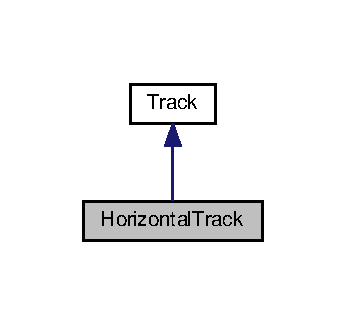
\includegraphics[width=174pt]{classKite_1_1HorizontalTrack__inherit__graph}
\end{center}
\end{figure}
\subsubsection*{Public Member Functions}
\begin{DoxyCompactItemize}
\item 
virtual bool \mbox{\hyperlink{classKite_1_1HorizontalTrack_a21b9cefd33ae22e4c2070ad441bdd30b}{is\+Horizontal}} () const
\item 
virtual bool \mbox{\hyperlink{classKite_1_1HorizontalTrack_abd54544ef1710ee4b67cfb021d73446c}{is\+Vertical}} () const
\item 
virtual unsigned int \mbox{\hyperlink{classKite_1_1HorizontalTrack_a0dd7cf705ace42c662c289955313b2e9}{get\+Direction}} () const
\item 
virtual \textbf{ Point} \mbox{\hyperlink{classKite_1_1HorizontalTrack_a6ab4f8026e4500918aa8721f1199f8b6}{get\+Position}} (\textbf{ Db\+U\+::\+Unit} coordinate) const
\end{DoxyCompactItemize}
\subsubsection*{Additional Inherited Members}


\subsubsection{Detailed Description}
Horizontal track managment. 

\subsubsection{Member Function Documentation}
\mbox{\Hypertarget{classKite_1_1HorizontalTrack_a21b9cefd33ae22e4c2070ad441bdd30b}\label{classKite_1_1HorizontalTrack_a21b9cefd33ae22e4c2070ad441bdd30b}} 
\index{Kite\+::\+Horizontal\+Track@{Kite\+::\+Horizontal\+Track}!is\+Horizontal@{is\+Horizontal}}
\index{is\+Horizontal@{is\+Horizontal}!Kite\+::\+Horizontal\+Track@{Kite\+::\+Horizontal\+Track}}
\paragraph{\texorpdfstring{is\+Horizontal()}{isHorizontal()}}
{\footnotesize\ttfamily bool is\+Horizontal (\begin{DoxyParamCaption}{ }\end{DoxyParamCaption}) const\hspace{0.3cm}{\ttfamily [virtual]}}

{\bfseries Returns\+:} {\bfseries true}. 

Implements \mbox{\hyperlink{classKite_1_1Track_a9d3db1f8a5aca58f8f54d291faebf873}{Track}}.

\mbox{\Hypertarget{classKite_1_1HorizontalTrack_abd54544ef1710ee4b67cfb021d73446c}\label{classKite_1_1HorizontalTrack_abd54544ef1710ee4b67cfb021d73446c}} 
\index{Kite\+::\+Horizontal\+Track@{Kite\+::\+Horizontal\+Track}!is\+Vertical@{is\+Vertical}}
\index{is\+Vertical@{is\+Vertical}!Kite\+::\+Horizontal\+Track@{Kite\+::\+Horizontal\+Track}}
\paragraph{\texorpdfstring{is\+Vertical()}{isVertical()}}
{\footnotesize\ttfamily bool is\+Vertical (\begin{DoxyParamCaption}{ }\end{DoxyParamCaption}) const\hspace{0.3cm}{\ttfamily [virtual]}}

{\bfseries Returns\+:} {\bfseries false}. 

Implements \mbox{\hyperlink{classKite_1_1Track_a6fa2bf0568a2b295dd7cd1f7207247d5}{Track}}.

\mbox{\Hypertarget{classKite_1_1HorizontalTrack_a0dd7cf705ace42c662c289955313b2e9}\label{classKite_1_1HorizontalTrack_a0dd7cf705ace42c662c289955313b2e9}} 
\index{Kite\+::\+Horizontal\+Track@{Kite\+::\+Horizontal\+Track}!get\+Direction@{get\+Direction}}
\index{get\+Direction@{get\+Direction}!Kite\+::\+Horizontal\+Track@{Kite\+::\+Horizontal\+Track}}
\paragraph{\texorpdfstring{get\+Direction()}{getDirection()}}
{\footnotesize\ttfamily unsigned int get\+Direction (\begin{DoxyParamCaption}{ }\end{DoxyParamCaption}) const\hspace{0.3cm}{\ttfamily [virtual]}}

{\bfseries Returns\+:} Katabatic\+::\+Kb\+Horizontal. 

Implements \mbox{\hyperlink{classKite_1_1Track_ae35b78590ed6aa546b626ef95f28c533}{Track}}.

\mbox{\Hypertarget{classKite_1_1HorizontalTrack_a6ab4f8026e4500918aa8721f1199f8b6}\label{classKite_1_1HorizontalTrack_a6ab4f8026e4500918aa8721f1199f8b6}} 
\index{Kite\+::\+Horizontal\+Track@{Kite\+::\+Horizontal\+Track}!get\+Position@{get\+Position}}
\index{get\+Position@{get\+Position}!Kite\+::\+Horizontal\+Track@{Kite\+::\+Horizontal\+Track}}
\paragraph{\texorpdfstring{get\+Position()}{getPosition()}}
{\footnotesize\ttfamily \textbf{ Point} get\+Position (\begin{DoxyParamCaption}\item[{\textbf{ Db\+U\+::\+Unit}}]{position }\end{DoxyParamCaption}) const\hspace{0.3cm}{\ttfamily [virtual]}}

{\bfseries Returns\+:} the point at {\ttfamily }(position,\mbox{\hyperlink{classKite_1_1Track_ab5b5aaa5b318369feee6003dbad039c2}{get\+Axis()}}). 

Implements \mbox{\hyperlink{classKite_1_1Track_a2a033f90e528d3d07aa33694dd733200}{Track}}.



The documentation for this class was generated from the following files\+:\begin{DoxyCompactItemize}
\item 
Horizontal\+Track.\+h\item 
Horizontal\+Track.\+cpp\item 
Horizontal\+Track.\+dox\end{DoxyCompactItemize}

\hypertarget{classKite_1_1RoutingEvent_1_1Key}{}\subsection{Routing\+Event\+:\+:Key Class Reference}
\label{classKite_1_1RoutingEvent_1_1Key}\index{Routing\+Event\+::\+Key@{Routing\+Event\+::\+Key}}


\hyperlink{classKite_1_1RoutingEvent}{Routing\+Event} cached key for maps.  


\subsubsection*{Public Member Functions}
\begin{DoxyCompactItemize}
\item 
void \hyperlink{classKite_1_1RoutingEvent_1_1Key_a398c66b87a5575dba86c92c7fad4a857}{update} (const \hyperlink{classKite_1_1RoutingEvent}{Routing\+Event} $\ast$)
\end{DoxyCompactItemize}


\subsubsection{Detailed Description}
\hyperlink{classKite_1_1RoutingEvent}{Routing\+Event} cached key for maps. 

The key is used as a cache in \hyperlink{classKite_1_1RoutingEvent}{Routing\+Event}, that is, the \hyperlink{classKite_1_1RoutingEvent}{Routing\+Event} attributes could be modificated without the key changing. It is important for the key to remain stable as it used in the various event queue as the sorting attribute. The key should be updated only when the \hyperlink{classKite_1_1RoutingEvent}{Routing\+Event} is temporarily whidrawn from the queue.

Cached attributes\+: (used in that lexicographical order for sorting)
\begin{DoxyItemize}
\item {\bfseries 1} -- {\ttfamily event\+Level}.
\item {\bfseries 2} -- {\ttfamily can\+Ripple}.
\item {\bfseries 3} -- {\ttfamily priority}.
\item {\bfseries 4} -- {\ttfamily length}.
\item {\bfseries 5} -- {\ttfamily is\+Horizontal}.
\item {\bfseries 6} -- {\ttfamily axis}.
\item {\bfseries 7} -- {\ttfamily sourceU}.
\item {\bfseries 8} -- {\ttfamily net} (name).
\item {\bfseries 9} -- {\ttfamily id}.
\item {\bfseries X} -- {\ttfamily slacken\+Strap} {\bfseries unused}.
\item {\bfseries X} -- {\ttfamily tracks\+Nb} {\bfseries unused}.
\end{DoxyItemize}

It is internally managed by \hyperlink{classKite_1_1RoutingEvent}{Routing\+Event} and the queue. 

\subsubsection{Member Function Documentation}
\mbox{\Hypertarget{classKite_1_1RoutingEvent_1_1Key_a398c66b87a5575dba86c92c7fad4a857}\label{classKite_1_1RoutingEvent_1_1Key_a398c66b87a5575dba86c92c7fad4a857}} 
\index{Kite\+::\+Routing\+Event\+::\+Key@{Kite\+::\+Routing\+Event\+::\+Key}!update@{update}}
\index{update@{update}!Kite\+::\+Routing\+Event\+::\+Key@{Kite\+::\+Routing\+Event\+::\+Key}}
\paragraph{\texorpdfstring{update()}{update()}}
{\footnotesize\ttfamily update (\begin{DoxyParamCaption}\item[{const \hyperlink{classKite_1_1RoutingEvent}{Routing\+Event} $\ast$}]{event }\end{DoxyParamCaption})}

Cache the value of the key from {\ttfamily event}. 

The documentation for this class was generated from the following files\+:\begin{DoxyCompactItemize}
\item 
Routing\+Event.\+h\item 
Routing\+Event.\+cpp\item 
Routing\+Event.\+dox\end{DoxyCompactItemize}

\hypertarget{classKite_1_1KiteEngine}{}\subsection{Kite\+Engine Class Reference}
\label{classKite_1_1KiteEngine}\index{Kite\+Engine@{Kite\+Engine}}


The \mbox{\hyperlink{namespaceKite}{Kite}} Tool.  




Inheritance diagram for Kite\+Engine\+:\nopagebreak
\begin{figure}[H]
\begin{center}
\leavevmode
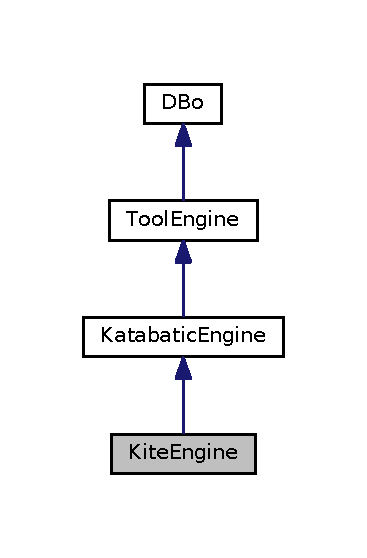
\includegraphics[width=168pt]{classKite_1_1KiteEngine__inherit__graph}
\end{center}
\end{figure}
\subsubsection*{Public Member Functions}
\begin{DoxyCompactItemize}
\item 
\textbf{ Katabatic\+Engine} $\ast$ \mbox{\hyperlink{classKite_1_1KiteEngine_a2313df62af32702cf749c15d349af5ea}{base}} ()
\item 
Configuration $\ast$ \mbox{\hyperlink{classKite_1_1KiteEngine_a1af1f95e771fba5c85a19ea2d686553a}{get\+Kite\+Configuration}} ()
\item 
virtual Configuration $\ast$ \mbox{\hyperlink{classKite_1_1KiteEngine_a9a7fbadfe526875680f698c76adfb128}{get\+Configuration}} ()
\item 
\textbf{ Net} $\ast$ \mbox{\hyperlink{classKite_1_1KiteEngine_aef6f41b0e8265ad574d1797f46ab9fa8}{get\+Blockage\+Net}} ()
\item 
bool \mbox{\hyperlink{classKite_1_1KiteEngine_ae88a4ccf0189655c785df38e5d75155c}{get\+Tool\+Success}} () const
\item 
unsigned long \mbox{\hyperlink{classKite_1_1KiteEngine_abb19e465ef249651bfc0efbe6f23ef1d}{get\+Events\+Limit}} () const
\item 
unsigned int \mbox{\hyperlink{classKite_1_1KiteEngine_aa9cc4f640a8b50dc1bcff8d938a09c3c}{get\+Ripup\+Limit}} (unsigned int type) const
\item 
unsigned int \mbox{\hyperlink{classKite_1_1KiteEngine_a1b4de41d8359251bcfbda288ec6bbbee}{get\+Ripup\+Cost}} () const
\end{DoxyCompactItemize}
\subsubsection*{Static Public Member Functions}
\begin{DoxyCompactItemize}
\item 
static const \textbf{ Name} \& \mbox{\hyperlink{classKite_1_1KiteEngine_a802eee6265da8d536db52d412f8a4afd}{static\+Get\+Name}} ()
\item 
static \mbox{\hyperlink{classKite_1_1KiteEngine}{Kite\+Engine}} $\ast$ \mbox{\hyperlink{classKite_1_1KiteEngine_a520d92a22c1becdc0fbbec927365db21}{create}} (\textbf{ Cell} $\ast$)
\item 
static \mbox{\hyperlink{classKite_1_1KiteEngine}{Kite\+Engine}} $\ast$ \mbox{\hyperlink{classKite_1_1KiteEngine_a9905ab1f7a970bc947adb8ddf54e55e1}{get}} (const \textbf{ Cell} $\ast$)
\end{DoxyCompactItemize}


\subsubsection{Detailed Description}
The \mbox{\hyperlink{namespaceKite}{Kite}} Tool. 

{\bfseries Lookup Mechanism}

Please look at \mbox{\hyperlink{classKite_1_1Session}{Kite\+::\+Session}} for an explanation of the lookup mechanism from \textbf{ Hurricane\+::\+Segment} or \textbf{ Katabatic\+::\+Auto\+Segment} to \mbox{\hyperlink{classKite_1_1TrackSegment}{Track\+Segment}}. 

\subsubsection{Member Function Documentation}
\mbox{\Hypertarget{classKite_1_1KiteEngine_a802eee6265da8d536db52d412f8a4afd}\label{classKite_1_1KiteEngine_a802eee6265da8d536db52d412f8a4afd}} 
\index{Kite\+::\+Kite\+Engine@{Kite\+::\+Kite\+Engine}!static\+Get\+Name@{static\+Get\+Name}}
\index{static\+Get\+Name@{static\+Get\+Name}!Kite\+::\+Kite\+Engine@{Kite\+::\+Kite\+Engine}}
\paragraph{\texorpdfstring{static\+Get\+Name()}{staticGetName()}}
{\footnotesize\ttfamily const \textbf{ Name} \& static\+Get\+Name (\begin{DoxyParamCaption}{ }\end{DoxyParamCaption})\hspace{0.3cm}{\ttfamily [static]}}

{\bfseries Returns\+:} The unique string identifier for the \mbox{\hyperlink{classKite_1_1KiteEngine}{Kite\+Engine}} class of Tool\+Engine. \mbox{\Hypertarget{classKite_1_1KiteEngine_a520d92a22c1becdc0fbbec927365db21}\label{classKite_1_1KiteEngine_a520d92a22c1becdc0fbbec927365db21}} 
\index{Kite\+::\+Kite\+Engine@{Kite\+::\+Kite\+Engine}!create@{create}}
\index{create@{create}!Kite\+::\+Kite\+Engine@{Kite\+::\+Kite\+Engine}}
\paragraph{\texorpdfstring{create()}{create()}}
{\footnotesize\ttfamily \mbox{\hyperlink{classKite_1_1KiteEngine}{Kite\+Engine}} $\ast$ create (\begin{DoxyParamCaption}\item[{\textbf{ Cell} $\ast$}]{cell }\end{DoxyParamCaption})\hspace{0.3cm}{\ttfamily [static]}}

Create a \mbox{\hyperlink{classKite_1_1KiteEngine}{Kite\+Engine}} on {\ttfamily cell}. \mbox{\Hypertarget{classKite_1_1KiteEngine_a9905ab1f7a970bc947adb8ddf54e55e1}\label{classKite_1_1KiteEngine_a9905ab1f7a970bc947adb8ddf54e55e1}} 
\index{Kite\+::\+Kite\+Engine@{Kite\+::\+Kite\+Engine}!get@{get}}
\index{get@{get}!Kite\+::\+Kite\+Engine@{Kite\+::\+Kite\+Engine}}
\paragraph{\texorpdfstring{get()}{get()}}
{\footnotesize\ttfamily \mbox{\hyperlink{classKite_1_1KiteEngine}{Kite\+Engine}} $\ast$ get (\begin{DoxyParamCaption}\item[{const \textbf{ Cell} $\ast$}]{cell }\end{DoxyParamCaption})\hspace{0.3cm}{\ttfamily [static]}}

{\bfseries Returns\+:} The \mbox{\hyperlink{classKite_1_1KiteEngine}{Kite\+Engine}} associated to {\ttfamily cell}. {\ttfamily N\+U\+LL} if there isn\textquotesingle{}t. \mbox{\Hypertarget{classKite_1_1KiteEngine_a2313df62af32702cf749c15d349af5ea}\label{classKite_1_1KiteEngine_a2313df62af32702cf749c15d349af5ea}} 
\index{Kite\+::\+Kite\+Engine@{Kite\+::\+Kite\+Engine}!base@{base}}
\index{base@{base}!Kite\+::\+Kite\+Engine@{Kite\+::\+Kite\+Engine}}
\paragraph{\texorpdfstring{base()}{base()}}
{\footnotesize\ttfamily \textbf{ Katabatic\+Engine} $\ast$ base (\begin{DoxyParamCaption}{ }\end{DoxyParamCaption})\hspace{0.3cm}{\ttfamily [inline]}}

{\bfseries Returns\+:} The \mbox{\hyperlink{classKite_1_1KiteEngine}{Kite\+Engine}}, casted as it\textquotesingle{}s base class (Katabatic\+Engine). \mbox{\Hypertarget{classKite_1_1KiteEngine_a1af1f95e771fba5c85a19ea2d686553a}\label{classKite_1_1KiteEngine_a1af1f95e771fba5c85a19ea2d686553a}} 
\index{Kite\+::\+Kite\+Engine@{Kite\+::\+Kite\+Engine}!get\+Kite\+Configuration@{get\+Kite\+Configuration}}
\index{get\+Kite\+Configuration@{get\+Kite\+Configuration}!Kite\+::\+Kite\+Engine@{Kite\+::\+Kite\+Engine}}
\paragraph{\texorpdfstring{get\+Kite\+Configuration()}{getKiteConfiguration()}}
{\footnotesize\ttfamily Configuration $\ast$ get\+Kite\+Configuration (\begin{DoxyParamCaption}{ }\end{DoxyParamCaption})\hspace{0.3cm}{\ttfamily [inline]}}

{\bfseries Returns\+:} The \mbox{\hyperlink{classKite_1_1KiteEngine}{Kite\+Engine}} configuration. The \mbox{\hyperlink{namespaceKite}{Kite}} Configuration is a derived class of Katabatic\+Configuration. \mbox{\Hypertarget{classKite_1_1KiteEngine_a9a7fbadfe526875680f698c76adfb128}\label{classKite_1_1KiteEngine_a9a7fbadfe526875680f698c76adfb128}} 
\index{Kite\+::\+Kite\+Engine@{Kite\+::\+Kite\+Engine}!get\+Configuration@{get\+Configuration}}
\index{get\+Configuration@{get\+Configuration}!Kite\+::\+Kite\+Engine@{Kite\+::\+Kite\+Engine}}
\paragraph{\texorpdfstring{get\+Configuration()}{getConfiguration()}}
{\footnotesize\ttfamily Configuration $\ast$ get\+Configuration (\begin{DoxyParamCaption}{ }\end{DoxyParamCaption})\hspace{0.3cm}{\ttfamily [virtual]}}

{\bfseries Returns\+:} The \mbox{\hyperlink{classKite_1_1KiteEngine}{Kite\+Engine}} configuration. 

Reimplemented from \textbf{ Katabatic\+Engine}.

\mbox{\Hypertarget{classKite_1_1KiteEngine_aef6f41b0e8265ad574d1797f46ab9fa8}\label{classKite_1_1KiteEngine_aef6f41b0e8265ad574d1797f46ab9fa8}} 
\index{Kite\+::\+Kite\+Engine@{Kite\+::\+Kite\+Engine}!get\+Blockage\+Net@{get\+Blockage\+Net}}
\index{get\+Blockage\+Net@{get\+Blockage\+Net}!Kite\+::\+Kite\+Engine@{Kite\+::\+Kite\+Engine}}
\paragraph{\texorpdfstring{get\+Blockage\+Net()}{getBlockageNet()}}
{\footnotesize\ttfamily \textbf{ Net} $\ast$ get\+Blockage\+Net (\begin{DoxyParamCaption}{ }\end{DoxyParamCaption})\hspace{0.3cm}{\ttfamily [inline]}}

{\bfseries Returns\+:} The Net which is used to mark the blockage segments. It\textquotesingle{}s not part of the Configuration {\itshape per se} but an isolated attribute. \mbox{\Hypertarget{classKite_1_1KiteEngine_ae88a4ccf0189655c785df38e5d75155c}\label{classKite_1_1KiteEngine_ae88a4ccf0189655c785df38e5d75155c}} 
\index{Kite\+::\+Kite\+Engine@{Kite\+::\+Kite\+Engine}!get\+Tool\+Success@{get\+Tool\+Success}}
\index{get\+Tool\+Success@{get\+Tool\+Success}!Kite\+::\+Kite\+Engine@{Kite\+::\+Kite\+Engine}}
\paragraph{\texorpdfstring{get\+Tool\+Success()}{getToolSuccess()}}
{\footnotesize\ttfamily bool get\+Tool\+Success (\begin{DoxyParamCaption}{ }\end{DoxyParamCaption}) const\hspace{0.3cm}{\ttfamily [inline]}}

{\bfseries Returns\+:} {\bfseries true} if the tool was successful, that is, all the Net were routeds. \mbox{\Hypertarget{classKite_1_1KiteEngine_abb19e465ef249651bfc0efbe6f23ef1d}\label{classKite_1_1KiteEngine_abb19e465ef249651bfc0efbe6f23ef1d}} 
\index{Kite\+::\+Kite\+Engine@{Kite\+::\+Kite\+Engine}!get\+Events\+Limit@{get\+Events\+Limit}}
\index{get\+Events\+Limit@{get\+Events\+Limit}!Kite\+::\+Kite\+Engine@{Kite\+::\+Kite\+Engine}}
\paragraph{\texorpdfstring{get\+Events\+Limit()}{getEventsLimit()}}
{\footnotesize\ttfamily unsigned long get\+Events\+Limit (\begin{DoxyParamCaption}{ }\end{DoxyParamCaption}) const\hspace{0.3cm}{\ttfamily [inline]}}

{\bfseries Returns\+:} The maximal number of allowed routing events. This limit is a security against infinite looping, be sure that it is great enough not to prevent normal routing completion. \mbox{\Hypertarget{classKite_1_1KiteEngine_aa9cc4f640a8b50dc1bcff8d938a09c3c}\label{classKite_1_1KiteEngine_aa9cc4f640a8b50dc1bcff8d938a09c3c}} 
\index{Kite\+::\+Kite\+Engine@{Kite\+::\+Kite\+Engine}!get\+Ripup\+Limit@{get\+Ripup\+Limit}}
\index{get\+Ripup\+Limit@{get\+Ripup\+Limit}!Kite\+::\+Kite\+Engine@{Kite\+::\+Kite\+Engine}}
\paragraph{\texorpdfstring{get\+Ripup\+Limit()}{getRipupLimit()}}
{\footnotesize\ttfamily unsigned long get\+Ripup\+Limit (\begin{DoxyParamCaption}\item[{unsigned int}]{type }\end{DoxyParamCaption}) const\hspace{0.3cm}{\ttfamily [inline]}}

{\bfseries Returns\+:} the maximum ripup allowed of a segment of {\ttfamily type}. 

Referenced by Manipulator\+::can\+Ripup(), and Segment\+Action\+::do\+Action().

\mbox{\Hypertarget{classKite_1_1KiteEngine_a1b4de41d8359251bcfbda288ec6bbbee}\label{classKite_1_1KiteEngine_a1b4de41d8359251bcfbda288ec6bbbee}} 
\index{Kite\+::\+Kite\+Engine@{Kite\+::\+Kite\+Engine}!get\+Ripup\+Cost@{get\+Ripup\+Cost}}
\index{get\+Ripup\+Cost@{get\+Ripup\+Cost}!Kite\+::\+Kite\+Engine@{Kite\+::\+Kite\+Engine}}
\paragraph{\texorpdfstring{get\+Ripup\+Cost()}{getRipupCost()}}
{\footnotesize\ttfamily unsigned long get\+Ripup\+Cost (\begin{DoxyParamCaption}{ }\end{DoxyParamCaption}) const\hspace{0.3cm}{\ttfamily [inline]}}

{\bfseries Returns\+:} the differential used while comparing two ripup costs. 

The documentation for this class was generated from the following files\+:\begin{DoxyCompactItemize}
\item 
Kite\+Engine.\+h\item 
Kite\+Engine.\+dox\end{DoxyCompactItemize}

\hypertarget{classKite_1_1Manipulator}{\subsection{Manipulator Class Reference}
\label{classKite_1_1Manipulator}\index{Manipulator@{Manipulator}}
}


Handle \hyperlink{classKite_1_1TrackElement}{Track\-Element} ripup \& topological modifications.  


\subsubsection*{Public Types}
\begin{DoxyCompactItemize}
\item 
enum \hyperlink{classKite_1_1Manipulator_a2af2ad6b6441614038caf59d04b3b217}{Function\-Flag} \{ \\*
\hyperlink{classKite_1_1Manipulator_a2af2ad6b6441614038caf59d04b3b217a6c00c46010d69247a3edc18b70d700fa}{To\-Ripup\-Limit} = 0x0001, 
\\*
\hyperlink{classKite_1_1Manipulator_a2af2ad6b6441614038caf59d04b3b217a41880b9f6652400677e21c8681f97675}{Allow\-Expand} = 0x0002, 
\\*
\hyperlink{classKite_1_1Manipulator_a2af2ad6b6441614038caf59d04b3b217a6d972ea7eb37fa1b58a9b3b805241ffd}{No\-Expand} = 0x0004, 
\\*
\hyperlink{classKite_1_1Manipulator_a2af2ad6b6441614038caf59d04b3b217acdaeb48fa352f2898aa225b618ca26d4}{Perpandiculars\-First} = 0x0008, 
\\*
\hyperlink{classKite_1_1Manipulator_a2af2ad6b6441614038caf59d04b3b217a6d49b8eaa1014c8d0169a22b2f675b4d}{To\-Move\-Up} = 0x0010, 
\\*
\hyperlink{classKite_1_1Manipulator_a2af2ad6b6441614038caf59d04b3b217a195c742e60b541424ed7b231e9736803}{Allow\-Local\-Move\-Up} = 0x0020, 
\\*
\hyperlink{classKite_1_1Manipulator_a2af2ad6b6441614038caf59d04b3b217ad16eaf385267fc57b0deba7cf2c49244}{Allow\-Terminal\-Move\-Up} = 0x0040, 
\\*
\hyperlink{classKite_1_1Manipulator_a2af2ad6b6441614038caf59d04b3b217a03c3d2cc0e6cfcf5cb2022d70a07f510}{Allow\-Short\-Pivot\-Up} = 0x0080, 
\\*
\hyperlink{classKite_1_1Manipulator_a2af2ad6b6441614038caf59d04b3b217ab254c6d61bbff307a2eb6592e1546131}{No\-Dogleg\-Reuse} = 0x0100, 
\\*
\hyperlink{classKite_1_1Manipulator_a2af2ad6b6441614038caf59d04b3b217ab525fc8ee72323922f991c26e098bd5a}{Left\-Axis\-Hint} = 0x0200, 
\\*
\hyperlink{classKite_1_1Manipulator_a2af2ad6b6441614038caf59d04b3b217a4412082ce8109b740834fe21e7a671fb}{Right\-Axis\-Hint} = 0x0400, 
\\*
\hyperlink{classKite_1_1Manipulator_a2af2ad6b6441614038caf59d04b3b217aeea607aabb515b52c3b29df30b079d21}{Not\-On\-Last\-Ripup} = 0x0800
 \}
\end{DoxyCompactItemize}
\subsubsection*{Public Member Functions}
\begin{DoxyCompactItemize}
\item 
\hyperlink{classKite_1_1Manipulator_ac02c770e24b6ff747867adcb7c4da92e}{Manipulator} (\hyperlink{classKite_1_1TrackElement}{Track\-Element} $\ast$, \hyperlink{classKite_1_1SegmentFsm}{Segment\-Fsm} \&)
\item 
\hyperlink{classKite_1_1TrackElement}{Track\-Element} $\ast$ \hyperlink{classKite_1_1Manipulator_ad2d369e354ca1f9ff118851da69c7efc}{get\-Segment} () const 
\item 
\hyperlink{classKite_1_1DataNegociate}{Data\-Negociate} $\ast$ \hyperlink{classKite_1_1Manipulator_aabb85a33d14a70586f4a2ca2dee566f0}{get\-Data} () const 
\item 
\hyperlink{classKite_1_1RoutingEvent}{Routing\-Event} $\ast$ \hyperlink{classKite_1_1Manipulator_a279d639cfaa447720f30991496f706a0}{get\-Event} () const 
\item 
bool \hyperlink{classKite_1_1Manipulator_aa1b59e12dd58840e11e1056cab4261b7}{can\-Ripup} (unsigned int flags=0) const 
\item 
bool \hyperlink{classKite_1_1Manipulator_af977361f4d90967fec7fbf1e778d01bb}{is\-Caged} ({\bf Db\-U\-::\-Unit}) const 
\item 
bool \hyperlink{classKite_1_1Manipulator_a370b5a5373d3019510d4ec22f44c76c2}{ripup} (unsigned int type, {\bf Db\-U\-::\-Unit} axis\-Hint=0)
\item 
bool \hyperlink{classKite_1_1Manipulator_a147c24aa53f561c10d5d24b82b03448a}{ripup\-Perpandiculars} (unsigned int flags=0)
\item 
void \hyperlink{classKite_1_1Manipulator_a9721ea909a9b11297dea855e1ba82a55}{repack\-Perpandiculars} ()
\item 
bool \hyperlink{classKite_1_1Manipulator_af46102d49a7aa0c163de1bf143807794}{ripple} ()
\item 
bool \hyperlink{classKite_1_1Manipulator_aa61f08642d981761687635be108b9837}{minimize} ()
\item 
bool \hyperlink{classKite_1_1Manipulator_a82897c077e4c0d4281c3dce3e37ab997}{slacken} (unsigned int flags=Kb\-No\-Flags)
\item 
bool \hyperlink{classKite_1_1Manipulator_ad590137c4e7e8d5ad2a6f510e0d70e81}{pivot\-Up} ()
\item 
bool \hyperlink{classKite_1_1Manipulator_ac3b48ad16d9b9b63d1c68e526ceb42e8}{pivot\-Down} ()
\item 
bool \hyperlink{classKite_1_1Manipulator_ac954731e16188acb6984f348bf2d9d20}{move\-Up} (unsigned int flags=0)
\item 
bool \hyperlink{classKite_1_1Manipulator_af4d93a43ea18ae124da71072c66d1e0a}{make\-Dogleg} ()
\item 
bool \hyperlink{classKite_1_1Manipulator_a97e56b831481ef65309f6e3b7e3f4f3d}{make\-Dogleg} ({\bf Db\-U\-::\-Unit})
\item 
bool \hyperlink{classKite_1_1Manipulator_af7b3305693dab195d0c5d075821fbb30}{make\-Dogleg} ({\bf Interval})
\item 
bool \hyperlink{classKite_1_1Manipulator_a8b5b69fd5762d5a0cbc4ceea4d1b68c1}{relax} ({\bf Interval}, unsigned int flags=\hyperlink{classKite_1_1Manipulator_a2af2ad6b6441614038caf59d04b3b217a41880b9f6652400677e21c8681f97675}{Allow\-Expand})
\item 
bool \hyperlink{classKite_1_1Manipulator_a7140b507da2cab137d968a037bed19df}{insert\-In\-Track} (size\-\_\-t)
\item 
bool \hyperlink{classKite_1_1Manipulator_aba69c61ccb330e26aaa8211f0454795f}{shrink\-To\-Track} (size\-\_\-t, unsigned int flags=0, {\bf Db\-U\-::\-Unit} left\-Axis\-Hint=0, {\bf Db\-U\-::\-Unit} right\-Axis\-Hint=0)
\item 
bool \hyperlink{classKite_1_1Manipulator_a76d3956660cfa624696e2a5f2916cd22}{force\-To\-Track} (size\-\_\-t)
\item 
bool \hyperlink{classKite_1_1Manipulator_add26b688d75a99a1ae781787eead08d5}{force\-Over\-Locals} ()
\end{DoxyCompactItemize}


\subsubsection{Detailed Description}
Handle \hyperlink{classKite_1_1TrackElement}{Track\-Element} ripup \& topological modifications. 

\hypertarget{classKite_1_1Manipulator_secManipStruct}{}\subsubsection{Manipulator Structure}\label{classKite_1_1Manipulator_secManipStruct}
A \hyperlink{classKite_1_1Manipulator}{Manipulator} basically binds together a \hyperlink{classKite_1_1TrackElement}{Track\-Element}, it's \hyperlink{classKite_1_1DataNegociate}{Data\-Negociate} and \hyperlink{classKite_1_1RoutingEvent}{Routing\-Event} (cached for fast access), and {\bfseries a} \hyperlink{classKite_1_1SegmentFsm}{Segment\-Fsm}.

{\itshape The \hyperlink{classKite_1_1TrackElement}{Track\-Element} may differs from the one of the \hyperlink{classKite_1_1SegmentFsm}{Segment\-Fsm}.} This can occurs when manipulating perpandiculars or segments from other nets in conflict. For example\-: \hyperlink{classKite_1_1Manipulator_af977361f4d90967fec7fbf1e778d01bb}{Manipulator\-::is\-Caged()}.

In the following documentation, the segment {\itshape which is associated to the \hyperlink{classKite_1_1SegmentFsm}{Segment\-Fsm}} will be called the {\itshape reference segment}.\hypertarget{classKite_1_1Manipulator_secManipDelayed}{}\subsubsection{Delayed Modifications}\label{classKite_1_1Manipulator_secManipDelayed}
It is important to note that when a \hyperlink{classKite_1_1Manipulator}{Manipulator} is called to modificate a \hyperlink{classKite_1_1TrackElement}{Track\-Element}, nothing is actually done by the \hyperlink{classKite_1_1Manipulator}{Manipulator} itself. Instead, the \hyperlink{classKite_1_1Manipulator}{Manipulator} create the relevant \hyperlink{classKite_1_1SegmentAction}{Segment\-Action} (s) that are stored in the \hyperlink{classKite_1_1SegmentFsm}{Segment\-Fsm}. The action themselves are done at the end of the \hyperlink{classKite_1_1SegmentFsm}{Segment\-Fsm} lifecycle (wrapped inside a \hyperlink{classKite_1_1Session}{Session}).

This is not true! When dogleg are created, the topology is immediatly modificated. That way of doing must be clarified. 

\subsubsection{Member Enumeration Documentation}
\hypertarget{classKite_1_1Manipulator_a2af2ad6b6441614038caf59d04b3b217}{\index{Kite\-::\-Manipulator@{Kite\-::\-Manipulator}!Function\-Flag@{Function\-Flag}}
\index{Function\-Flag@{Function\-Flag}!Kite::Manipulator@{Kite\-::\-Manipulator}}
\paragraph[{Function\-Flag}]{\setlength{\rightskip}{0pt plus 5cm}enum {\bf Function\-Flag}}}\label{classKite_1_1Manipulator_a2af2ad6b6441614038caf59d04b3b217}
The various flags that can be passed to the \hyperlink{classKite_1_1Manipulator}{Manipulator} methods. \begin{Desc}
\item[Enumerator]\par
\begin{description}
\index{To\-Ripup\-Limit@{To\-Ripup\-Limit}!Kite\-::\-Manipulator@{Kite\-::\-Manipulator}}\index{Kite\-::\-Manipulator@{Kite\-::\-Manipulator}!To\-Ripup\-Limit@{To\-Ripup\-Limit}}\item[{\em 
\hypertarget{classKite_1_1Manipulator_a2af2ad6b6441614038caf59d04b3b217a6c00c46010d69247a3edc18b70d700fa}{To\-Ripup\-Limit}\label{classKite_1_1Manipulator_a2af2ad6b6441614038caf59d04b3b217a6c00c46010d69247a3edc18b70d700fa}
}]The ripup limit must be immediatly to it's limit for the current state. \index{Allow\-Expand@{Allow\-Expand}!Kite\-::\-Manipulator@{Kite\-::\-Manipulator}}\index{Kite\-::\-Manipulator@{Kite\-::\-Manipulator}!Allow\-Expand@{Allow\-Expand}}\item[{\em 
\hypertarget{classKite_1_1Manipulator_a2af2ad6b6441614038caf59d04b3b217a41880b9f6652400677e21c8681f97675}{Allow\-Expand}\label{classKite_1_1Manipulator_a2af2ad6b6441614038caf59d04b3b217a41880b9f6652400677e21c8681f97675}
}]Allow break points for dogleg not to be exactly on the requested position. Meaning that they are moved to the least congested G\-Cell. \index{No\-Expand@{No\-Expand}!Kite\-::\-Manipulator@{Kite\-::\-Manipulator}}\index{Kite\-::\-Manipulator@{Kite\-::\-Manipulator}!No\-Expand@{No\-Expand}}\item[{\em 
\hypertarget{classKite_1_1Manipulator_a2af2ad6b6441614038caf59d04b3b217a6d972ea7eb37fa1b58a9b3b805241ffd}{No\-Expand}\label{classKite_1_1Manipulator_a2af2ad6b6441614038caf59d04b3b217a6d972ea7eb37fa1b58a9b3b805241ffd}
}]Breakpoints for dogleg are kept right where they are requested. \index{Perpandiculars\-First@{Perpandiculars\-First}!Kite\-::\-Manipulator@{Kite\-::\-Manipulator}}\index{Kite\-::\-Manipulator@{Kite\-::\-Manipulator}!Perpandiculars\-First@{Perpandiculars\-First}}\item[{\em 
\hypertarget{classKite_1_1Manipulator_a2af2ad6b6441614038caf59d04b3b217acdaeb48fa352f2898aa225b618ca26d4}{Perpandiculars\-First}\label{classKite_1_1Manipulator_a2af2ad6b6441614038caf59d04b3b217acdaeb48fa352f2898aa225b618ca26d4}
}]Reorder the events so that perpandiculars segments are re-\/processed before their reference segment. By default this is the other way around. \index{To\-Move\-Up@{To\-Move\-Up}!Kite\-::\-Manipulator@{Kite\-::\-Manipulator}}\index{Kite\-::\-Manipulator@{Kite\-::\-Manipulator}!To\-Move\-Up@{To\-Move\-Up}}\item[{\em 
\hypertarget{classKite_1_1Manipulator_a2af2ad6b6441614038caf59d04b3b217a6d49b8eaa1014c8d0169a22b2f675b4d}{To\-Move\-Up}\label{classKite_1_1Manipulator_a2af2ad6b6441614038caf59d04b3b217a6d49b8eaa1014c8d0169a22b2f675b4d}
}]Try to move up ripped up segments. \index{Allow\-Local\-Move\-Up@{Allow\-Local\-Move\-Up}!Kite\-::\-Manipulator@{Kite\-::\-Manipulator}}\index{Kite\-::\-Manipulator@{Kite\-::\-Manipulator}!Allow\-Local\-Move\-Up@{Allow\-Local\-Move\-Up}}\item[{\em 
\hypertarget{classKite_1_1Manipulator_a2af2ad6b6441614038caf59d04b3b217a195c742e60b541424ed7b231e9736803}{Allow\-Local\-Move\-Up}\label{classKite_1_1Manipulator_a2af2ad6b6441614038caf59d04b3b217a195c742e60b541424ed7b231e9736803}
}]Allow local segments to be moved up (forbidden by default). \index{Allow\-Terminal\-Move\-Up@{Allow\-Terminal\-Move\-Up}!Kite\-::\-Manipulator@{Kite\-::\-Manipulator}}\index{Kite\-::\-Manipulator@{Kite\-::\-Manipulator}!Allow\-Terminal\-Move\-Up@{Allow\-Terminal\-Move\-Up}}\item[{\em 
\hypertarget{classKite_1_1Manipulator_a2af2ad6b6441614038caf59d04b3b217ad16eaf385267fc57b0deba7cf2c49244}{Allow\-Terminal\-Move\-Up}\label{classKite_1_1Manipulator_a2af2ad6b6441614038caf59d04b3b217ad16eaf385267fc57b0deba7cf2c49244}
}]Allow terminal segments to be moved up (forbidden by default). \index{Allow\-Short\-Pivot\-Up@{Allow\-Short\-Pivot\-Up}!Kite\-::\-Manipulator@{Kite\-::\-Manipulator}}\index{Kite\-::\-Manipulator@{Kite\-::\-Manipulator}!Allow\-Short\-Pivot\-Up@{Allow\-Short\-Pivot\-Up}}\item[{\em 
\hypertarget{classKite_1_1Manipulator_a2af2ad6b6441614038caf59d04b3b217a03c3d2cc0e6cfcf5cb2022d70a07f510}{Allow\-Short\-Pivot\-Up}\label{classKite_1_1Manipulator_a2af2ad6b6441614038caf59d04b3b217a03c3d2cc0e6cfcf5cb2022d70a07f510}
}]Allow short segment yo be pivoted up. \index{No\-Dogleg\-Reuse@{No\-Dogleg\-Reuse}!Kite\-::\-Manipulator@{Kite\-::\-Manipulator}}\index{Kite\-::\-Manipulator@{Kite\-::\-Manipulator}!No\-Dogleg\-Reuse@{No\-Dogleg\-Reuse}}\item[{\em 
\hypertarget{classKite_1_1Manipulator_a2af2ad6b6441614038caf59d04b3b217ab254c6d61bbff307a2eb6592e1546131}{No\-Dogleg\-Reuse}\label{classKite_1_1Manipulator_a2af2ad6b6441614038caf59d04b3b217ab254c6d61bbff307a2eb6592e1546131}
}]When creating a dogleg, the default behavior is {\itshape not} to create a new one if there's already one in the same G\-Cell. If this flag is set, a second dogleg will be created. \index{Left\-Axis\-Hint@{Left\-Axis\-Hint}!Kite\-::\-Manipulator@{Kite\-::\-Manipulator}}\index{Kite\-::\-Manipulator@{Kite\-::\-Manipulator}!Left\-Axis\-Hint@{Left\-Axis\-Hint}}\item[{\em 
\hypertarget{classKite_1_1Manipulator_a2af2ad6b6441614038caf59d04b3b217ab525fc8ee72323922f991c26e098bd5a}{Left\-Axis\-Hint}\label{classKite_1_1Manipulator_a2af2ad6b6441614038caf59d04b3b217ab525fc8ee72323922f991c26e098bd5a}
}]An explicit left axis hint has been supplied as argument. \index{Right\-Axis\-Hint@{Right\-Axis\-Hint}!Kite\-::\-Manipulator@{Kite\-::\-Manipulator}}\index{Kite\-::\-Manipulator@{Kite\-::\-Manipulator}!Right\-Axis\-Hint@{Right\-Axis\-Hint}}\item[{\em 
\hypertarget{classKite_1_1Manipulator_a2af2ad6b6441614038caf59d04b3b217a4412082ce8109b740834fe21e7a671fb}{Right\-Axis\-Hint}\label{classKite_1_1Manipulator_a2af2ad6b6441614038caf59d04b3b217a4412082ce8109b740834fe21e7a671fb}
}]An explicit right axis hint has been supplied as argument. \index{Not\-On\-Last\-Ripup@{Not\-On\-Last\-Ripup}!Kite\-::\-Manipulator@{Kite\-::\-Manipulator}}\index{Kite\-::\-Manipulator@{Kite\-::\-Manipulator}!Not\-On\-Last\-Ripup@{Not\-On\-Last\-Ripup}}\item[{\em 
\hypertarget{classKite_1_1Manipulator_a2af2ad6b6441614038caf59d04b3b217aeea607aabb515b52c3b29df30b079d21}{Not\-On\-Last\-Ripup}\label{classKite_1_1Manipulator_a2af2ad6b6441614038caf59d04b3b217aeea607aabb515b52c3b29df30b079d21}
}]The reference segment has still more than one ripup to go for the given state. \end{description}
\end{Desc}


\subsubsection{Constructor \& Destructor Documentation}
\hypertarget{classKite_1_1Manipulator_ac02c770e24b6ff747867adcb7c4da92e}{\index{Kite\-::\-Manipulator@{Kite\-::\-Manipulator}!Manipulator@{Manipulator}}
\index{Manipulator@{Manipulator}!Kite::Manipulator@{Kite\-::\-Manipulator}}
\paragraph[{Manipulator}]{\setlength{\rightskip}{0pt plus 5cm}{\bf Manipulator} (
\begin{DoxyParamCaption}
\item[{{\bf Track\-Element} $\ast$}]{segment, }
\item[{{\bf Segment\-Fsm} \&}]{fsm}
\end{DoxyParamCaption}
)}}\label{classKite_1_1Manipulator_ac02c770e24b6ff747867adcb7c4da92e}

\begin{DoxyParams}{Parameters}
{\em segment} & The \hyperlink{classKite_1_1TrackElement}{Track\-Element} to manipulate. \\
\hline
{\em fsm} & The associated \hyperlink{classKite_1_1SegmentFsm}{Segment\-Fsm}.\\
\hline
\end{DoxyParams}
Construct a new \hyperlink{classKite_1_1Manipulator}{Manipulator} on {\ttfamily segment}. 

Referenced by Manipulator\-::force\-Over\-Locals(), Manipulator\-::force\-To\-Track(), Manipulator\-::insert\-In\-Track(), Manipulator\-::ripup\-Perpandiculars(), and Manipulator\-::shrink\-To\-Track().



\subsubsection{Member Function Documentation}
\hypertarget{classKite_1_1Manipulator_ad2d369e354ca1f9ff118851da69c7efc}{\index{Kite\-::\-Manipulator@{Kite\-::\-Manipulator}!get\-Segment@{get\-Segment}}
\index{get\-Segment@{get\-Segment}!Kite::Manipulator@{Kite\-::\-Manipulator}}
\paragraph[{get\-Segment}]{\setlength{\rightskip}{0pt plus 5cm}{\bf Track\-Element} $\ast$ get\-Segment (
\begin{DoxyParamCaption}
{}
\end{DoxyParamCaption}
) const\hspace{0.3cm}{\ttfamily [inline]}}}\label{classKite_1_1Manipulator_ad2d369e354ca1f9ff118851da69c7efc}
{\bfseries Returns\-:} The working \hyperlink{classKite_1_1TrackElement}{Track\-Element}. \hypertarget{classKite_1_1Manipulator_aabb85a33d14a70586f4a2ca2dee566f0}{\index{Kite\-::\-Manipulator@{Kite\-::\-Manipulator}!get\-Data@{get\-Data}}
\index{get\-Data@{get\-Data}!Kite::Manipulator@{Kite\-::\-Manipulator}}
\paragraph[{get\-Data}]{\setlength{\rightskip}{0pt plus 5cm}{\bf Data\-Negociate} $\ast$ get\-Data (
\begin{DoxyParamCaption}
{}
\end{DoxyParamCaption}
) const\hspace{0.3cm}{\ttfamily [inline]}}}\label{classKite_1_1Manipulator_aabb85a33d14a70586f4a2ca2dee566f0}
{\bfseries Returns\-:} The \hyperlink{classKite_1_1DataNegociate}{Data\-Negociate} of the \hyperlink{classKite_1_1TrackElement}{Track\-Element} (act as a cache). \hypertarget{classKite_1_1Manipulator_a279d639cfaa447720f30991496f706a0}{\index{Kite\-::\-Manipulator@{Kite\-::\-Manipulator}!get\-Event@{get\-Event}}
\index{get\-Event@{get\-Event}!Kite::Manipulator@{Kite\-::\-Manipulator}}
\paragraph[{get\-Event}]{\setlength{\rightskip}{0pt plus 5cm}{\bf Routing\-Event} $\ast$ get\-Event (
\begin{DoxyParamCaption}
{}
\end{DoxyParamCaption}
) const\hspace{0.3cm}{\ttfamily [inline]}}}\label{classKite_1_1Manipulator_a279d639cfaa447720f30991496f706a0}
{\bfseries Returns\-:} The \hyperlink{classKite_1_1RoutingEvent}{Routing\-Event} associated to the \hyperlink{classKite_1_1TrackElement}{Track\-Element} (act as a cache). \hypertarget{classKite_1_1Manipulator_aa1b59e12dd58840e11e1056cab4261b7}{\index{Kite\-::\-Manipulator@{Kite\-::\-Manipulator}!can\-Ripup@{can\-Ripup}}
\index{can\-Ripup@{can\-Ripup}!Kite::Manipulator@{Kite\-::\-Manipulator}}
\paragraph[{can\-Ripup}]{\setlength{\rightskip}{0pt plus 5cm}bool can\-Ripup (
\begin{DoxyParamCaption}
\item[{unsigned int}]{flags = {\ttfamily 0}}
\end{DoxyParamCaption}
) const}}\label{classKite_1_1Manipulator_aa1b59e12dd58840e11e1056cab4261b7}
{\bfseries Returns\-:} {\bfseries true} if the maximum ripup, for the given \hyperlink{classKite_1_1SegmentFsm_a5d74787dedbc4e11c1ab15bf487e61f8}{Segment\-Fsm\-::\-State} has not been reached. If {\ttfamily flags} contains Manipulator\-::\-Has\-Next\-Ripup, return {\bfseries true} {\bfseries only} if it still have at least one ripup to go. 

Referenced by Manipulator\-::force\-To\-Track(), and Manipulator\-::ripup().

\hypertarget{classKite_1_1Manipulator_af977361f4d90967fec7fbf1e778d01bb}{\index{Kite\-::\-Manipulator@{Kite\-::\-Manipulator}!is\-Caged@{is\-Caged}}
\index{is\-Caged@{is\-Caged}!Kite::Manipulator@{Kite\-::\-Manipulator}}
\paragraph[{is\-Caged}]{\setlength{\rightskip}{0pt plus 5cm}bool is\-Caged (
\begin{DoxyParamCaption}
\item[{{\bf Db\-U\-::\-Unit}}]{axis}
\end{DoxyParamCaption}
) const}}\label{classKite_1_1Manipulator_af977361f4d90967fec7fbf1e778d01bb}
{\bfseries Returns\-:} {\bfseries true} if the segment is enclosed (in it's \hyperlink{classKite_1_1Track}{Track}) by two fixed or blockage segments which at least one is closer than 10 lambdas from {\ttfamily axis}. Mostly used to know if a perpandicular is actually restricting the axis span of a reference segment. 

Referenced by Manipulator\-::ripup\-Perpandiculars().

\hypertarget{classKite_1_1Manipulator_a370b5a5373d3019510d4ec22f44c76c2}{\index{Kite\-::\-Manipulator@{Kite\-::\-Manipulator}!ripup@{ripup}}
\index{ripup@{ripup}!Kite::Manipulator@{Kite\-::\-Manipulator}}
\paragraph[{ripup}]{\setlength{\rightskip}{0pt plus 5cm}bool ripup (
\begin{DoxyParamCaption}
\item[{unsigned int}]{type, }
\item[{{\bf Db\-U\-::\-Unit}}]{axis\-Hint = {\ttfamily 0}}
\end{DoxyParamCaption}
)}}\label{classKite_1_1Manipulator_a370b5a5373d3019510d4ec22f44c76c2}

\begin{DoxyParams}{Parameters}
{\em type} & The type of ripup action. \\
\hline
{\em axis\-Hint} & An indication as where to move the riped up segment. \\
\hline
\end{DoxyParams}
\begin{DoxyReturn}{Returns}
{\bfseries true} if the operation has succedeed.
\end{DoxyReturn}
If the \hyperlink{classKite_1_1TrackElement}{Track\-Element} can be ripped up, schedule a ripup action, possibly with a hint for the preferred axis position. 

Referenced by Manipulator\-::force\-Over\-Locals(), Manipulator\-::force\-To\-Track(), Manipulator\-::insert\-In\-Track(), and Manipulator\-::ripup\-Perpandiculars().

\hypertarget{classKite_1_1Manipulator_a147c24aa53f561c10d5d24b82b03448a}{\index{Kite\-::\-Manipulator@{Kite\-::\-Manipulator}!ripup\-Perpandiculars@{ripup\-Perpandiculars}}
\index{ripup\-Perpandiculars@{ripup\-Perpandiculars}!Kite::Manipulator@{Kite\-::\-Manipulator}}
\paragraph[{ripup\-Perpandiculars}]{\setlength{\rightskip}{0pt plus 5cm}bool ripup\-Perpandiculars (
\begin{DoxyParamCaption}
\item[{unsigned int}]{flags = {\ttfamily 0}}
\end{DoxyParamCaption}
)}}\label{classKite_1_1Manipulator_a147c24aa53f561c10d5d24b82b03448a}
Schedule a ripup of all the perpandiculars of the reference segment. {\ttfamily flags} that modificate the behavior\-:
\begin{DoxyItemize}
\item \hyperlink{classKite_1_1Manipulator_a2af2ad6b6441614038caf59d04b3b217acdaeb48fa352f2898aa225b618ca26d4}{Manipulator\-::\-Perpandiculars\-First} \-: the queue will be reordered so that all the perpandiculars are re-\/processed (placed) before the reference segment.
\item \hyperlink{classKite_1_1Manipulator_a2af2ad6b6441614038caf59d04b3b217a6c00c46010d69247a3edc18b70d700fa}{Manipulator\-::\-To\-Ripup\-Limit} \-: the ripup count of the reference segment is set to the limit (i.\-e. only one more attempt before a slackening occurs).
\end{DoxyItemize}

The method will fails (return {\bfseries false}) if at least one perpandicular can't be changed of track (i.\-e. ripped up) {\bfseries and} none of it's neighbors could be ripped up either. Meaning that the free span on that track cannot be changed. 

Referenced by Segment\-Fsm\-::conflict\-Solve\-By\-Placeds().

\hypertarget{classKite_1_1Manipulator_a9721ea909a9b11297dea855e1ba82a55}{\index{Kite\-::\-Manipulator@{Kite\-::\-Manipulator}!repack\-Perpandiculars@{repack\-Perpandiculars}}
\index{repack\-Perpandiculars@{repack\-Perpandiculars}!Kite::Manipulator@{Kite\-::\-Manipulator}}
\paragraph[{repack\-Perpandiculars}]{\setlength{\rightskip}{0pt plus 5cm}bool repack\-Perpandiculars (
\begin{DoxyParamCaption}
{}
\end{DoxyParamCaption}
)}}\label{classKite_1_1Manipulator_a9721ea909a9b11297dea855e1ba82a55}
Ripup all the perpandiculars of the reference segment, except fixed or globals. The reference segment is rescheduled first (before it's perpandicular).

This function may be used to find a better placement, maximizing the overlap of the various perpandiculars.

Ripup all perpandiculars and the reference segment itself for a complete re-\/placement. The reference segment will be reprocessed {\itshape before} it's perpandiculars. \hypertarget{classKite_1_1Manipulator_af46102d49a7aa0c163de1bf143807794}{\index{Kite\-::\-Manipulator@{Kite\-::\-Manipulator}!ripple@{ripple}}
\index{ripple@{ripple}!Kite::Manipulator@{Kite\-::\-Manipulator}}
\paragraph[{ripple}]{\setlength{\rightskip}{0pt plus 5cm}bool ripple (
\begin{DoxyParamCaption}
{}
\end{DoxyParamCaption}
)}}\label{classKite_1_1Manipulator_af46102d49a7aa0c163de1bf143807794}
{\bfseries Returns\-:} true if the reference segment is local.

Applies only on reference segments that are of local type. Tries to make room for the reference segment by ripping up it's neigbors on the parallels tracks. On a vertical plane, left neigbors are shifted one track left (trough axis hint) and right ones, one track right. Note that they are ripped up and the shift is just a hint, there's no guarantee that the router can honor it. 

Referenced by Manipulator\-::ripup\-Perpandiculars().

\hypertarget{classKite_1_1Manipulator_aa61f08642d981761687635be108b9837}{\index{Kite\-::\-Manipulator@{Kite\-::\-Manipulator}!minimize@{minimize}}
\index{minimize@{minimize}!Kite::Manipulator@{Kite\-::\-Manipulator}}
\paragraph[{minimize}]{\setlength{\rightskip}{0pt plus 5cm}bool minimize (
\begin{DoxyParamCaption}
{}
\end{DoxyParamCaption}
)}}\label{classKite_1_1Manipulator_aa61f08642d981761687635be108b9837}
{\bfseries Returns\-:} true if the reference segment can be mimized in a suitable track hole.

Compute the miminal span of the reference segment, summing up contraints from source anchor and target anchors (if any) and perpandiculars. Then find holes in the avalaible tracks, and check if one is suitable for the miminized segment (try first the biggest hole).

This operation can only be called once on a segment (a flag is set in the event). \hypertarget{classKite_1_1Manipulator_a82897c077e4c0d4281c3dce3e37ab997}{\index{Kite\-::\-Manipulator@{Kite\-::\-Manipulator}!slacken@{slacken}}
\index{slacken@{slacken}!Kite::Manipulator@{Kite\-::\-Manipulator}}
\paragraph[{slacken}]{\setlength{\rightskip}{0pt plus 5cm}bool slacken (
\begin{DoxyParamCaption}
\item[{unsigned int}]{flags = {\ttfamily KbNoFlags}}
\end{DoxyParamCaption}
)}}\label{classKite_1_1Manipulator_a82897c077e4c0d4281c3dce3e37ab997}
Simple proxy towards Track\-Element\-::slacken().

To be reviewed. \hypertarget{classKite_1_1Manipulator_ad590137c4e7e8d5ad2a6f510e0d70e81}{\index{Kite\-::\-Manipulator@{Kite\-::\-Manipulator}!pivot\-Up@{pivot\-Up}}
\index{pivot\-Up@{pivot\-Up}!Kite::Manipulator@{Kite\-::\-Manipulator}}
\paragraph[{pivot\-Up}]{\setlength{\rightskip}{0pt plus 5cm}bool pivot\-Up (
\begin{DoxyParamCaption}
{}
\end{DoxyParamCaption}
)}}\label{classKite_1_1Manipulator_ad590137c4e7e8d5ad2a6f510e0d70e81}
Tries to move up the reference segment. The segment will be moved up only if a half track is free (for a local) or a full track is free (for a global).

This function do not modifies/create perpandiculars. 

Referenced by Segment\-Fsm\-::solve\-Full\-Blockages().

\hypertarget{classKite_1_1Manipulator_ac3b48ad16d9b9b63d1c68e526ceb42e8}{\index{Kite\-::\-Manipulator@{Kite\-::\-Manipulator}!pivot\-Down@{pivot\-Down}}
\index{pivot\-Down@{pivot\-Down}!Kite::Manipulator@{Kite\-::\-Manipulator}}
\paragraph[{pivot\-Down}]{\setlength{\rightskip}{0pt plus 5cm}bool pivot\-Down (
\begin{DoxyParamCaption}
{}
\end{DoxyParamCaption}
)}}\label{classKite_1_1Manipulator_ac3b48ad16d9b9b63d1c68e526ceb42e8}
Tries to move down the reference segment. The segment will be moved up only if {\itshape two} track are free (whether global or local). Is is more restrictive than \hyperlink{classKite_1_1Manipulator_ad590137c4e7e8d5ad2a6f510e0d70e81}{Manipulator\-::pivot\-Up()}.

This function do not modifies/create perpandiculars. \hypertarget{classKite_1_1Manipulator_ac954731e16188acb6984f348bf2d9d20}{\index{Kite\-::\-Manipulator@{Kite\-::\-Manipulator}!move\-Up@{move\-Up}}
\index{move\-Up@{move\-Up}!Kite::Manipulator@{Kite\-::\-Manipulator}}
\paragraph[{move\-Up}]{\setlength{\rightskip}{0pt plus 5cm}bool move\-Up (
\begin{DoxyParamCaption}
\item[{unsigned int}]{flags = {\ttfamily 0}}
\end{DoxyParamCaption}
)}}\label{classKite_1_1Manipulator_ac954731e16188acb6984f348bf2d9d20}
Tries to move up a segment, if there is enough space in the \hyperlink{classKite_1_1RoutingPlane}{Routing\-Plane} above and in the same direction.

This function may modificate perpandiculars in order to maintain connexity.

To be reviewed. 

Referenced by Segment\-Fsm\-::solve\-Full\-Blockages().

\hypertarget{classKite_1_1Manipulator_af4d93a43ea18ae124da71072c66d1e0a}{\index{Kite\-::\-Manipulator@{Kite\-::\-Manipulator}!make\-Dogleg@{make\-Dogleg}}
\index{make\-Dogleg@{make\-Dogleg}!Kite::Manipulator@{Kite\-::\-Manipulator}}
\paragraph[{make\-Dogleg}]{\setlength{\rightskip}{0pt plus 5cm}bool make\-Dogleg (
\begin{DoxyParamCaption}
{}
\end{DoxyParamCaption}
)}}\label{classKite_1_1Manipulator_af4d93a43ea18ae124da71072c66d1e0a}
{\bfseries Returns\-:} {\bfseries false} if the segment is {\itshape not} local or the dogleg cannot be done.

For {\itshape local} reference segment only, look in the first track candidate for other segment overlapping and break the reference accordingly. \hypertarget{classKite_1_1Manipulator_a97e56b831481ef65309f6e3b7e3f4f3d}{\index{Kite\-::\-Manipulator@{Kite\-::\-Manipulator}!make\-Dogleg@{make\-Dogleg}}
\index{make\-Dogleg@{make\-Dogleg}!Kite::Manipulator@{Kite\-::\-Manipulator}}
\paragraph[{make\-Dogleg}]{\setlength{\rightskip}{0pt plus 5cm}bool make\-Dogleg (
\begin{DoxyParamCaption}
\item[{{\bf Db\-U\-::\-Unit}}]{position}
\end{DoxyParamCaption}
)}}\label{classKite_1_1Manipulator_a97e56b831481ef65309f6e3b7e3f4f3d}
Create a dogleg in the G\-Cell under {\ttfamily position}. \hypertarget{classKite_1_1Manipulator_af7b3305693dab195d0c5d075821fbb30}{\index{Kite\-::\-Manipulator@{Kite\-::\-Manipulator}!make\-Dogleg@{make\-Dogleg}}
\index{make\-Dogleg@{make\-Dogleg}!Kite::Manipulator@{Kite\-::\-Manipulator}}
\paragraph[{make\-Dogleg}]{\setlength{\rightskip}{0pt plus 5cm}bool make\-Dogleg (
\begin{DoxyParamCaption}
\item[{{\bf Interval}}]{overlap}
\end{DoxyParamCaption}
)}}\label{classKite_1_1Manipulator_af7b3305693dab195d0c5d075821fbb30}
Create a dogleg to avoid the obstructed interval {\ttfamily overlap}. \hypertarget{classKite_1_1Manipulator_a8b5b69fd5762d5a0cbc4ceea4d1b68c1}{\index{Kite\-::\-Manipulator@{Kite\-::\-Manipulator}!relax@{relax}}
\index{relax@{relax}!Kite::Manipulator@{Kite\-::\-Manipulator}}
\paragraph[{relax}]{\setlength{\rightskip}{0pt plus 5cm}bool relax (
\begin{DoxyParamCaption}
\item[{{\bf Interval}}]{overlap, }
\item[{unsigned int}]{flags = {\ttfamily {\bf Allow\-Expand}}}
\end{DoxyParamCaption}
)}}\label{classKite_1_1Manipulator_a8b5b69fd5762d5a0cbc4ceea4d1b68c1}
Break the reference segment so it can detour around the interval {\ttfamily overlap}. If {\ttfamily overlap} is completly enclosed inside the span of the reference segment two dogleg will be created. If the overlap occurs only on one side of the reference segment, only one dogleg will be created.

If {\ttfamily flags} contains \hyperlink{classKite_1_1Manipulator_a2af2ad6b6441614038caf59d04b3b217a41880b9f6652400677e21c8681f97675}{Manipulator\-::\-Allow\-Expand}, the dogleg are not created exactly at the edges of the overlap but on the lowest density G\-Cell (outside the overlap interval).

The axis of the created dogleg are sets so that the broken part of the segment completly enclose {\ttfamily overlap}. That is, the orignal segment no longer intersect with {\ttfamily overlap}. So the min dogleg is pushed to the left and the max to the right if they are in the same G\-Cell as the min/max of {\ttfamily overlap}. Otherwise (they have been expanded), they are put in the center of the G\-Cell.

We do not allow to dogleg twice in the same G\-Cell, so if min or max is in respectively the first or last G\-Cell, it is not done. Moreover if there is only one dogleg {\itshape and} it is in the first or last G\-Cell, the relax method is cancelled (and returns {\bfseries false}). It means that this is the segment which is likely to be enclosed inside {\ttfamily overlap}.

{\bfseries Important\-:} The doglegs are created immediatly and not in a delayed fashion like the \hyperlink{classKite_1_1SegmentAction}{Segment\-Action}.

    \hypertarget{classKite_1_1Manipulator_a7140b507da2cab137d968a037bed19df}{\index{Kite\-::\-Manipulator@{Kite\-::\-Manipulator}!insert\-In\-Track@{insert\-In\-Track}}
\index{insert\-In\-Track@{insert\-In\-Track}!Kite::Manipulator@{Kite\-::\-Manipulator}}
\paragraph[{insert\-In\-Track}]{\setlength{\rightskip}{0pt plus 5cm}bool insert\-In\-Track (
\begin{DoxyParamCaption}
\item[{size\-\_\-t}]{i}
\end{DoxyParamCaption}
)}}\label{classKite_1_1Manipulator_a7140b507da2cab137d968a037bed19df}
Try to insert the reference segment in the track at index {\ttfamily i} (in the cost table from \hyperlink{classKite_1_1SegmentFsm}{Segment\-Fsm}). The insertion is done by ripping up overlapping segment or shrinking them to left/right if possible.

This operation ripup the processed segment neighbors (and their perpandiculars). \hypertarget{classKite_1_1Manipulator_aba69c61ccb330e26aaa8211f0454795f}{\index{Kite\-::\-Manipulator@{Kite\-::\-Manipulator}!shrink\-To\-Track@{shrink\-To\-Track}}
\index{shrink\-To\-Track@{shrink\-To\-Track}!Kite::Manipulator@{Kite\-::\-Manipulator}}
\paragraph[{shrink\-To\-Track}]{\setlength{\rightskip}{0pt plus 5cm}bool shrink\-To\-Track (
\begin{DoxyParamCaption}
\item[{size\-\_\-t}]{i, }
\item[{unsigned int}]{flags = {\ttfamily 0}, }
\item[{{\bf Db\-U\-::\-Unit}}]{left\-Axis\-Hint = {\ttfamily 0}, }
\item[{{\bf Db\-U\-::\-Unit}}]{right\-Axis\-Hint = {\ttfamily 0}}
\end{DoxyParamCaption}
)}}\label{classKite_1_1Manipulator_aba69c61ccb330e26aaa8211f0454795f}
Attempt to minimize the reference segment to fit into the track. For this operation to succeed, the minimal span of the segment must not overlap any other segment already in the track. To reach the minimal span the perpandiculars are ripped up with an axis hint which is the center of the minimal span or the explicit value given as arguments {\ttfamily left\-Axis\-Hint} and {\ttfamily right\-Axis\-Hint} if {\ttfamily flags} contains respectively \hyperlink{classKite_1_1Manipulator_a2af2ad6b6441614038caf59d04b3b217ab525fc8ee72323922f991c26e098bd5a}{Manipulator\-::\-Left\-Axis\-Hint} or \hyperlink{classKite_1_1Manipulator_a2af2ad6b6441614038caf59d04b3b217a4412082ce8109b740834fe21e7a671fb}{Manipulator\-::\-Right\-Axis\-Hint}.

This operation ripup the processed segment itself and its perpandiculars. \hypertarget{classKite_1_1Manipulator_a76d3956660cfa624696e2a5f2916cd22}{\index{Kite\-::\-Manipulator@{Kite\-::\-Manipulator}!force\-To\-Track@{force\-To\-Track}}
\index{force\-To\-Track@{force\-To\-Track}!Kite::Manipulator@{Kite\-::\-Manipulator}}
\paragraph[{force\-To\-Track}]{\setlength{\rightskip}{0pt plus 5cm}bool force\-To\-Track (
\begin{DoxyParamCaption}
\item[{size\-\_\-t}]{i}
\end{DoxyParamCaption}
)}}\label{classKite_1_1Manipulator_a76d3956660cfa624696e2a5f2916cd22}
Try to insert the reference segment in the track at index {\ttfamily i} (in the cost table from \hyperlink{classKite_1_1SegmentFsm}{Segment\-Fsm}). The insertion is done by {\itshape forcibly} ripping up the overlapping segments {\bfseries and} their perpandiculars.

This operation ripup the processed segment neighbors (and their perpandiculars). \hypertarget{classKite_1_1Manipulator_add26b688d75a99a1ae781787eead08d5}{\index{Kite\-::\-Manipulator@{Kite\-::\-Manipulator}!force\-Over\-Locals@{force\-Over\-Locals}}
\index{force\-Over\-Locals@{force\-Over\-Locals}!Kite::Manipulator@{Kite\-::\-Manipulator}}
\paragraph[{force\-Over\-Locals}]{\setlength{\rightskip}{0pt plus 5cm}bool force\-Over\-Locals (
\begin{DoxyParamCaption}
{}
\end{DoxyParamCaption}
)}}\label{classKite_1_1Manipulator_add26b688d75a99a1ae781787eead08d5}
Loop over all the candidate tracks and, insert in the first which all conflicting segments are locals (rip them up). 

The documentation for this class was generated from the following files\-:\begin{DoxyCompactItemize}
\item 
Manipulator.\-h\item 
Manipulator.\-cpp\item 
Manipulator.\-dox\end{DoxyCompactItemize}

\hypertarget{classKite_1_1NegociateWindow}{}\subsection{Negociate\+Window Class Reference}
\label{classKite_1_1NegociateWindow}\index{Negociate\+Window@{Negociate\+Window}}


Perform the routing, main \hyperlink{classKite_1_1RoutingEvent}{Routing\+Event} manager.  


\subsubsection*{Public Types}
\begin{DoxyCompactItemize}
\item 
enum \hyperlink{classKite_1_1NegociateWindow_aca8133200c1122e29b87b314d82604eb}{Stage} \{ \newline
\hyperlink{classKite_1_1NegociateWindow_aca8133200c1122e29b87b314d82604eba19ccda3133337a5db697480ebfd6097f}{Negociation} = 1, 
\newline
\hyperlink{classKite_1_1NegociateWindow_aca8133200c1122e29b87b314d82604ebabdd3263d9492edf336ac52b4a9776b82}{Packing} = 2
 \}
\end{DoxyCompactItemize}
\subsubsection*{Public Member Functions}
\begin{DoxyCompactItemize}
\item 
void \hyperlink{classKite_1_1NegociateWindow_a3a80b6032f86a56bec74609034b3246f}{destroy} ()
\item 
bool \hyperlink{classKite_1_1NegociateWindow_aa1a08014471e19352a5efdabad3a87cb}{is\+Interrupted} () const
\item 
\hyperlink{classKite_1_1KiteEngine}{Kite\+Engine} $\ast$ \hyperlink{classKite_1_1NegociateWindow_af7373bd3a4ee8fcf28a316230ed37fc0}{get\+Kite\+Engine} () const
\item 
\textbf{ Hurricane\+::\+Cell} $\ast$ \hyperlink{classKite_1_1NegociateWindow_a5ea0f667687d3a832f8c9806ccbe6792}{get\+Cell} () const
\item 
const Katabatic\+::\+G\+Cell\+Vector \& \hyperlink{classKite_1_1NegociateWindow_ad8902daa6817d4275be5e3a37eb24424}{get\+G\+Cells} () const
\item 
\hyperlink{classKite_1_1RoutingEventQueue}{Routing\+Event\+Queue} \& \hyperlink{classKite_1_1NegociateWindow_a80fc29623500b168c49ba14c49a00a76}{get\+Event\+Queue} ()
\item 
\hyperlink{classKite_1_1RoutingEventHistory}{Routing\+Event\+History} \& \hyperlink{classKite_1_1NegociateWindow_a990d738cf85fa016589edaa08d736d4f}{get\+Event\+History} ()
\item 
\hyperlink{classKite_1_1RoutingEventLoop}{Routing\+Event\+Loop} \& \hyperlink{classKite_1_1NegociateWindow_a9a41d40e5e378b9bcb99048262ec15a6}{get\+Event\+Loop} ()
\item 
\hyperlink{classKite_1_1NegociateWindow_aca8133200c1122e29b87b314d82604eb}{Stage} \hyperlink{classKite_1_1NegociateWindow_aeb77fbb60f78895b010f7a12658864a6}{get\+Stage} () const
\item 
void \hyperlink{classKite_1_1NegociateWindow_a329dbc5bc549e3fe354996368dbf7113}{set\+G\+Cells} (const Katabatic\+::\+G\+Cell\+Vector \&)
\item 
void \hyperlink{classKite_1_1NegociateWindow_a7c0d10dab2d32985e942b7678dcccafd}{set\+Interrupt} (bool)
\item 
void \hyperlink{classKite_1_1NegociateWindow_aad6b43971b936f7ea003d3ad0fd07532}{set\+Stage} (\hyperlink{classKite_1_1NegociateWindow_aca8133200c1122e29b87b314d82604eb}{Stage})
\item 
double \hyperlink{classKite_1_1NegociateWindow_a4936106670361df6b6f3ef0b6088c9dc}{compute\+Wirelength} ()
\item 
\hyperlink{classKite_1_1TrackElement}{Track\+Element} $\ast$ \hyperlink{classKite_1_1NegociateWindow_a7bf31fcd4e4007e62454689ef7c553fc}{create\+Track\+Segment} (\textbf{ Auto\+Segment} $\ast$, unsigned int flags)
\item 
void \hyperlink{classKite_1_1NegociateWindow_a51ba8e6a122c0cb93174027658cade63}{add\+Routing\+Event} (\hyperlink{classKite_1_1TrackElement}{Track\+Element} $\ast$, unsigned int level)
\item 
void \hyperlink{classKite_1_1NegociateWindow_acad8f73494d122463d65797d337ce275}{reschedule\+Event} (\hyperlink{classKite_1_1RoutingEvent}{Routing\+Event} $\ast$, unsigned int level)
\item 
void \hyperlink{classKite_1_1NegociateWindow_a61e848b73b597f54e2e83e13eb70ff83}{run} (unsigned int flags)
\item 
void \hyperlink{classKite_1_1NegociateWindow_a8d3dfaa30cedabd6b64977827ac989d8}{print\+Statistics} () const
\end{DoxyCompactItemize}
\subsubsection*{Static Public Member Functions}
\begin{DoxyCompactItemize}
\item 
static \hyperlink{classKite_1_1NegociateWindow}{Negociate\+Window} $\ast$ \hyperlink{classKite_1_1NegociateWindow_ad9c37ea1398a6dfa332cb297141dc1c4}{create} (\hyperlink{classKite_1_1KiteEngine}{Kite\+Engine} $\ast$)
\end{DoxyCompactItemize}


\subsubsection{Detailed Description}
Perform the routing, main \hyperlink{classKite_1_1RoutingEvent}{Routing\+Event} manager. 

This object perform the routing. That is creates all the initial \hyperlink{classKite_1_1RoutingEvent}{Routing\+Event}, load them into the queue and then process the queue until it is empty, that is, the routing is finished.

This object is the owner of the \hyperlink{classKite_1_1RoutingEventQueue}{Routing\+Event\+Queue}, \hyperlink{classKite_1_1RoutingEventHistory}{Routing\+Event\+History} and \hyperlink{classKite_1_1RoutingEventLoop}{Routing\+Event\+Loop} used all troughout \hyperlink{classKite_1_1RoutingEvent}{Routing\+Event} and \hyperlink{classKite_1_1SegmentFsm}{Segment\+Fsm}. 

\subsubsection{Member Enumeration Documentation}
\mbox{\Hypertarget{classKite_1_1NegociateWindow_aca8133200c1122e29b87b314d82604eb}\label{classKite_1_1NegociateWindow_aca8133200c1122e29b87b314d82604eb}} 
\index{Kite\+::\+Negociate\+Window@{Kite\+::\+Negociate\+Window}!Stage@{Stage}}
\index{Stage@{Stage}!Kite\+::\+Negociate\+Window@{Kite\+::\+Negociate\+Window}}
\paragraph{\texorpdfstring{Stage}{Stage}}
{\footnotesize\ttfamily enum \hyperlink{classKite_1_1NegociateWindow_aca8133200c1122e29b87b314d82604eb}{Stage}}

The state under which the router is operating. \begin{DoxyEnumFields}{Enumerator}
\raisebox{\heightof{T}}[0pt][0pt]{\index{Negociation@{Negociation}!Kite\+::\+Negociate\+Window@{Kite\+::\+Negociate\+Window}}\index{Kite\+::\+Negociate\+Window@{Kite\+::\+Negociate\+Window}!Negociation@{Negociation}}}\mbox{\Hypertarget{classKite_1_1NegociateWindow_aca8133200c1122e29b87b314d82604eba19ccda3133337a5db697480ebfd6097f}\label{classKite_1_1NegociateWindow_aca8133200c1122e29b87b314d82604eba19ccda3133337a5db697480ebfd6097f}} 
Negociation&The normal mode, priority negociation with ripup. \\
\hline

\raisebox{\heightof{T}}[0pt][0pt]{\index{Packing@{Packing}!Kite\+::\+Negociate\+Window@{Kite\+::\+Negociate\+Window}}\index{Kite\+::\+Negociate\+Window@{Kite\+::\+Negociate\+Window}!Packing@{Packing}}}\mbox{\Hypertarget{classKite_1_1NegociateWindow_aca8133200c1122e29b87b314d82604ebabdd3263d9492edf336ac52b4a9776b82}\label{classKite_1_1NegociateWindow_aca8133200c1122e29b87b314d82604ebabdd3263d9492edf336ac52b4a9776b82}} 
Packing&Try to find a better placement for segment but just by looking for other fully free spaces. No ripup is performed. \\
\hline

\end{DoxyEnumFields}


\subsubsection{Member Function Documentation}
\mbox{\Hypertarget{classKite_1_1NegociateWindow_ad9c37ea1398a6dfa332cb297141dc1c4}\label{classKite_1_1NegociateWindow_ad9c37ea1398a6dfa332cb297141dc1c4}} 
\index{Kite\+::\+Negociate\+Window@{Kite\+::\+Negociate\+Window}!create@{create}}
\index{create@{create}!Kite\+::\+Negociate\+Window@{Kite\+::\+Negociate\+Window}}
\paragraph{\texorpdfstring{create()}{create()}}
{\footnotesize\ttfamily create (\begin{DoxyParamCaption}\item[{\hyperlink{classKite_1_1KiteEngine}{Kite\+Engine} $\ast$}]{kite }\end{DoxyParamCaption})\hspace{0.3cm}{\ttfamily [static]}}

The publicly avalaible contructor. Route the whole are defined by the \hyperlink{namespaceKite}{Kite} associated Cell abutment box. \mbox{\Hypertarget{classKite_1_1NegociateWindow_a3a80b6032f86a56bec74609034b3246f}\label{classKite_1_1NegociateWindow_a3a80b6032f86a56bec74609034b3246f}} 
\index{Kite\+::\+Negociate\+Window@{Kite\+::\+Negociate\+Window}!destroy@{destroy}}
\index{destroy@{destroy}!Kite\+::\+Negociate\+Window@{Kite\+::\+Negociate\+Window}}
\paragraph{\texorpdfstring{destroy()}{destroy()}}
{\footnotesize\ttfamily void destroy (\begin{DoxyParamCaption}{ }\end{DoxyParamCaption})}

The publicly avalaible destructor. \mbox{\Hypertarget{classKite_1_1NegociateWindow_aa1a08014471e19352a5efdabad3a87cb}\label{classKite_1_1NegociateWindow_aa1a08014471e19352a5efdabad3a87cb}} 
\index{Kite\+::\+Negociate\+Window@{Kite\+::\+Negociate\+Window}!is\+Interrupted@{is\+Interrupted}}
\index{is\+Interrupted@{is\+Interrupted}!Kite\+::\+Negociate\+Window@{Kite\+::\+Negociate\+Window}}
\paragraph{\texorpdfstring{is\+Interrupted()}{isInterrupted()}}
{\footnotesize\ttfamily bool is\+Interrupted (\begin{DoxyParamCaption}{ }\end{DoxyParamCaption}) const\hspace{0.3cm}{\ttfamily [inline]}}

{\bfseries Returns\+:} {\bfseries true} if the \hyperlink{classKite_1_1NegociateWindow}{Negociate\+Window} has received an interrupt request. \mbox{\Hypertarget{classKite_1_1NegociateWindow_af7373bd3a4ee8fcf28a316230ed37fc0}\label{classKite_1_1NegociateWindow_af7373bd3a4ee8fcf28a316230ed37fc0}} 
\index{Kite\+::\+Negociate\+Window@{Kite\+::\+Negociate\+Window}!get\+Kite\+Engine@{get\+Kite\+Engine}}
\index{get\+Kite\+Engine@{get\+Kite\+Engine}!Kite\+::\+Negociate\+Window@{Kite\+::\+Negociate\+Window}}
\paragraph{\texorpdfstring{get\+Kite\+Engine()}{getKiteEngine()}}
{\footnotesize\ttfamily \hyperlink{classKite_1_1KiteEngine}{Kite\+Engine} $\ast$ get\+Kite\+Engine (\begin{DoxyParamCaption}{ }\end{DoxyParamCaption}) const\hspace{0.3cm}{\ttfamily [inline]}}

{\bfseries Returns\+:} The associated \hyperlink{classKite_1_1KiteEngine}{Kite\+Engine}. \mbox{\Hypertarget{classKite_1_1NegociateWindow_a5ea0f667687d3a832f8c9806ccbe6792}\label{classKite_1_1NegociateWindow_a5ea0f667687d3a832f8c9806ccbe6792}} 
\index{Kite\+::\+Negociate\+Window@{Kite\+::\+Negociate\+Window}!get\+Cell@{get\+Cell}}
\index{get\+Cell@{get\+Cell}!Kite\+::\+Negociate\+Window@{Kite\+::\+Negociate\+Window}}
\paragraph{\texorpdfstring{get\+Cell()}{getCell()}}
{\footnotesize\ttfamily \textbf{ Hurricane\+::\+Cell} $\ast$ get\+Cell (\begin{DoxyParamCaption}{ }\end{DoxyParamCaption}) const}

{\bfseries Returns\+:} The associated Cell. \mbox{\Hypertarget{classKite_1_1NegociateWindow_ad8902daa6817d4275be5e3a37eb24424}\label{classKite_1_1NegociateWindow_ad8902daa6817d4275be5e3a37eb24424}} 
\index{Kite\+::\+Negociate\+Window@{Kite\+::\+Negociate\+Window}!get\+G\+Cells@{get\+G\+Cells}}
\index{get\+G\+Cells@{get\+G\+Cells}!Kite\+::\+Negociate\+Window@{Kite\+::\+Negociate\+Window}}
\paragraph{\texorpdfstring{get\+G\+Cells()}{getGCells()}}
{\footnotesize\ttfamily const Katabatic\+::\+G\+Cell\+Vector \& get\+G\+Cells (\begin{DoxyParamCaption}{ }\end{DoxyParamCaption}) const\hspace{0.3cm}{\ttfamily [inline]}}

{\bfseries Returns\+:} A Copy of the vector of G\+Cell from Katabatic\+Engine. The vector is copied but not the G\+Cell themselves (shallow copy). \mbox{\Hypertarget{classKite_1_1NegociateWindow_a80fc29623500b168c49ba14c49a00a76}\label{classKite_1_1NegociateWindow_a80fc29623500b168c49ba14c49a00a76}} 
\index{Kite\+::\+Negociate\+Window@{Kite\+::\+Negociate\+Window}!get\+Event\+Queue@{get\+Event\+Queue}}
\index{get\+Event\+Queue@{get\+Event\+Queue}!Kite\+::\+Negociate\+Window@{Kite\+::\+Negociate\+Window}}
\paragraph{\texorpdfstring{get\+Event\+Queue()}{getEventQueue()}}
{\footnotesize\ttfamily \hyperlink{classKite_1_1RoutingEventQueue}{Routing\+Event\+Queue} \& get\+Event\+Queue (\begin{DoxyParamCaption}{ }\end{DoxyParamCaption})\hspace{0.3cm}{\ttfamily [inline]}}

{\bfseries Returns\+:} The \hyperlink{classKite_1_1RoutingEventQueue}{Routing\+Event\+Queue}. \mbox{\Hypertarget{classKite_1_1NegociateWindow_a990d738cf85fa016589edaa08d736d4f}\label{classKite_1_1NegociateWindow_a990d738cf85fa016589edaa08d736d4f}} 
\index{Kite\+::\+Negociate\+Window@{Kite\+::\+Negociate\+Window}!get\+Event\+History@{get\+Event\+History}}
\index{get\+Event\+History@{get\+Event\+History}!Kite\+::\+Negociate\+Window@{Kite\+::\+Negociate\+Window}}
\paragraph{\texorpdfstring{get\+Event\+History()}{getEventHistory()}}
{\footnotesize\ttfamily \hyperlink{classKite_1_1RoutingEventHistory}{Routing\+Event\+History} \& get\+Event\+History (\begin{DoxyParamCaption}{ }\end{DoxyParamCaption})\hspace{0.3cm}{\ttfamily [inline]}}

{\bfseries Returns\+:} The \hyperlink{classKite_1_1RoutingEventHistory}{Routing\+Event\+History}. \mbox{\Hypertarget{classKite_1_1NegociateWindow_a9a41d40e5e378b9bcb99048262ec15a6}\label{classKite_1_1NegociateWindow_a9a41d40e5e378b9bcb99048262ec15a6}} 
\index{Kite\+::\+Negociate\+Window@{Kite\+::\+Negociate\+Window}!get\+Event\+Loop@{get\+Event\+Loop}}
\index{get\+Event\+Loop@{get\+Event\+Loop}!Kite\+::\+Negociate\+Window@{Kite\+::\+Negociate\+Window}}
\paragraph{\texorpdfstring{get\+Event\+Loop()}{getEventLoop()}}
{\footnotesize\ttfamily \hyperlink{classKite_1_1RoutingEventLoop}{Routing\+Event\+Loop} \& get\+Event\+Loop (\begin{DoxyParamCaption}{ }\end{DoxyParamCaption})\hspace{0.3cm}{\ttfamily [inline]}}

{\bfseries Returns\+:} The \hyperlink{classKite_1_1RoutingEventLoop}{Routing\+Event\+Loop}. \mbox{\Hypertarget{classKite_1_1NegociateWindow_aeb77fbb60f78895b010f7a12658864a6}\label{classKite_1_1NegociateWindow_aeb77fbb60f78895b010f7a12658864a6}} 
\index{Kite\+::\+Negociate\+Window@{Kite\+::\+Negociate\+Window}!get\+Stage@{get\+Stage}}
\index{get\+Stage@{get\+Stage}!Kite\+::\+Negociate\+Window@{Kite\+::\+Negociate\+Window}}
\paragraph{\texorpdfstring{get\+Stage()}{getStage()}}
{\footnotesize\ttfamily \hyperlink{classKite_1_1NegociateWindow_aca8133200c1122e29b87b314d82604eb}{Stage} get\+Stage (\begin{DoxyParamCaption}{ }\end{DoxyParamCaption}) const\hspace{0.3cm}{\ttfamily [inline]}}

{\bfseries Returns\+:} The stage (Negicate\+Window\+::\+Stage) into which the \hyperlink{classKite_1_1NegociateWindow}{Negociate\+Window} is running. 

Referenced by Routing\+Event\+::reschedule(), and Routing\+Event\+::set\+Axis\+Hint\+From\+Parent().

\mbox{\Hypertarget{classKite_1_1NegociateWindow_a329dbc5bc549e3fe354996368dbf7113}\label{classKite_1_1NegociateWindow_a329dbc5bc549e3fe354996368dbf7113}} 
\index{Kite\+::\+Negociate\+Window@{Kite\+::\+Negociate\+Window}!set\+G\+Cells@{set\+G\+Cells}}
\index{set\+G\+Cells@{set\+G\+Cells}!Kite\+::\+Negociate\+Window@{Kite\+::\+Negociate\+Window}}
\paragraph{\texorpdfstring{set\+G\+Cells()}{setGCells()}}
{\footnotesize\ttfamily void set\+G\+Cells (\begin{DoxyParamCaption}\item[{const Katabatic\+::\+G\+Cell\+Vector \&}]{v }\end{DoxyParamCaption})}

Sets the G\+Cell vector from Katabatic\+Engine (perform a shallow copy). \mbox{\Hypertarget{classKite_1_1NegociateWindow_a7c0d10dab2d32985e942b7678dcccafd}\label{classKite_1_1NegociateWindow_a7c0d10dab2d32985e942b7678dcccafd}} 
\index{Kite\+::\+Negociate\+Window@{Kite\+::\+Negociate\+Window}!set\+Interrupt@{set\+Interrupt}}
\index{set\+Interrupt@{set\+Interrupt}!Kite\+::\+Negociate\+Window@{Kite\+::\+Negociate\+Window}}
\paragraph{\texorpdfstring{set\+Interrupt()}{setInterrupt()}}
{\footnotesize\ttfamily void set\+Interrupt (\begin{DoxyParamCaption}\item[{bool}]{state }\end{DoxyParamCaption})\hspace{0.3cm}{\ttfamily [inline]}}

Sets or unset the interruption flag. \mbox{\Hypertarget{classKite_1_1NegociateWindow_aad6b43971b936f7ea003d3ad0fd07532}\label{classKite_1_1NegociateWindow_aad6b43971b936f7ea003d3ad0fd07532}} 
\index{Kite\+::\+Negociate\+Window@{Kite\+::\+Negociate\+Window}!set\+Stage@{set\+Stage}}
\index{set\+Stage@{set\+Stage}!Kite\+::\+Negociate\+Window@{Kite\+::\+Negociate\+Window}}
\paragraph{\texorpdfstring{set\+Stage()}{setStage()}}
{\footnotesize\ttfamily void set\+Stage (\begin{DoxyParamCaption}\item[{\hyperlink{classKite_1_1NegociateWindow_aca8133200c1122e29b87b314d82604eb}{Stage}}]{stage }\end{DoxyParamCaption})\hspace{0.3cm}{\ttfamily [inline]}}

Set the stage (\hyperlink{classKite_1_1NegociateWindow_aca8133200c1122e29b87b314d82604eb}{Negociate\+Window\+::\+Stage}) under which we are running. \mbox{\Hypertarget{classKite_1_1NegociateWindow_a4936106670361df6b6f3ef0b6088c9dc}\label{classKite_1_1NegociateWindow_a4936106670361df6b6f3ef0b6088c9dc}} 
\index{Kite\+::\+Negociate\+Window@{Kite\+::\+Negociate\+Window}!compute\+Wirelength@{compute\+Wirelength}}
\index{compute\+Wirelength@{compute\+Wirelength}!Kite\+::\+Negociate\+Window@{Kite\+::\+Negociate\+Window}}
\paragraph{\texorpdfstring{compute\+Wirelength()}{computeWirelength()}}
{\footnotesize\ttfamily double compute\+Wirelength (\begin{DoxyParamCaption}{ }\end{DoxyParamCaption})}

Compute the total wirelength of the circuit. It is not completly accurate because overlaps are not took into accounts. \mbox{\Hypertarget{classKite_1_1NegociateWindow_a7bf31fcd4e4007e62454689ef7c553fc}\label{classKite_1_1NegociateWindow_a7bf31fcd4e4007e62454689ef7c553fc}} 
\index{Kite\+::\+Negociate\+Window@{Kite\+::\+Negociate\+Window}!create\+Track\+Segment@{create\+Track\+Segment}}
\index{create\+Track\+Segment@{create\+Track\+Segment}!Kite\+::\+Negociate\+Window@{Kite\+::\+Negociate\+Window}}
\paragraph{\texorpdfstring{create\+Track\+Segment()}{createTrackSegment()}}
{\footnotesize\ttfamily \hyperlink{classKite_1_1TrackElement}{Track\+Element} $\ast$ create\+Track\+Segment (\begin{DoxyParamCaption}\item[{\textbf{ Auto\+Segment} $\ast$}]{auto\+Segment,  }\item[{unsigned int}]{flags }\end{DoxyParamCaption})}

Build a \hyperlink{classKite_1_1TrackSegment}{Track\+Segment} from the \textbf{ Katabatic\+::\+Auto\+Segment}. If {\ttfamily flags} contains Kite\+::\+Kt\+Loading\+Stage then assume that we are in the initial loading stage (constructor). \mbox{\Hypertarget{classKite_1_1NegociateWindow_a51ba8e6a122c0cb93174027658cade63}\label{classKite_1_1NegociateWindow_a51ba8e6a122c0cb93174027658cade63}} 
\index{Kite\+::\+Negociate\+Window@{Kite\+::\+Negociate\+Window}!add\+Routing\+Event@{add\+Routing\+Event}}
\index{add\+Routing\+Event@{add\+Routing\+Event}!Kite\+::\+Negociate\+Window@{Kite\+::\+Negociate\+Window}}
\paragraph{\texorpdfstring{add\+Routing\+Event()}{addRoutingEvent()}}
{\footnotesize\ttfamily void add\+Routing\+Event (\begin{DoxyParamCaption}\item[{\hyperlink{classKite_1_1TrackElement}{Track\+Element} $\ast$}]{segment,  }\item[{unsigned int}]{level }\end{DoxyParamCaption})}

Create a new \hyperlink{classKite_1_1RoutingEvent}{Routing\+Event} from \hyperlink{classKite_1_1TrackElement}{Track\+Element} (if it doesn\textquotesingle{}t already exists) and insert it into the queue with priority {\ttfamily level}. 

Referenced by Track\+Segment\+::reschedule().

\mbox{\Hypertarget{classKite_1_1NegociateWindow_acad8f73494d122463d65797d337ce275}\label{classKite_1_1NegociateWindow_acad8f73494d122463d65797d337ce275}} 
\index{Kite\+::\+Negociate\+Window@{Kite\+::\+Negociate\+Window}!reschedule\+Event@{reschedule\+Event}}
\index{reschedule\+Event@{reschedule\+Event}!Kite\+::\+Negociate\+Window@{Kite\+::\+Negociate\+Window}}
\paragraph{\texorpdfstring{reschedule\+Event()}{rescheduleEvent()}}
{\footnotesize\ttfamily void reschedule\+Event (\begin{DoxyParamCaption}\item[{\hyperlink{classKite_1_1RoutingEvent}{Routing\+Event} $\ast$}]{event,  }\item[{unsigned int}]{level }\end{DoxyParamCaption})\hspace{0.3cm}{\ttfamily [inline]}}

Reschedule an event into the queue, with priority {\ttfamily level}. 

Referenced by Track\+Segment\+::reschedule().

\mbox{\Hypertarget{classKite_1_1NegociateWindow_a61e848b73b597f54e2e83e13eb70ff83}\label{classKite_1_1NegociateWindow_a61e848b73b597f54e2e83e13eb70ff83}} 
\index{Kite\+::\+Negociate\+Window@{Kite\+::\+Negociate\+Window}!run@{run}}
\index{run@{run}!Kite\+::\+Negociate\+Window@{Kite\+::\+Negociate\+Window}}
\paragraph{\texorpdfstring{run()}{run()}}
{\footnotesize\ttfamily void run (\begin{DoxyParamCaption}\item[{unsigned int}]{flags }\end{DoxyParamCaption})}

Perform the routing.

{\ttfamily slow\+Motion} is not implemented yet. \mbox{\Hypertarget{classKite_1_1NegociateWindow_a8d3dfaa30cedabd6b64977827ac989d8}\label{classKite_1_1NegociateWindow_a8d3dfaa30cedabd6b64977827ac989d8}} 
\index{Kite\+::\+Negociate\+Window@{Kite\+::\+Negociate\+Window}!print\+Statistics@{print\+Statistics}}
\index{print\+Statistics@{print\+Statistics}!Kite\+::\+Negociate\+Window@{Kite\+::\+Negociate\+Window}}
\paragraph{\texorpdfstring{print\+Statistics()}{printStatistics()}}
{\footnotesize\ttfamily void print\+Statistics (\begin{DoxyParamCaption}{ }\end{DoxyParamCaption}) const}

Display some statistics about the routing, compute the internal complete statistics. 

The documentation for this class was generated from the following files\+:\begin{DoxyCompactItemize}
\item 
Negociate\+Window.\+h\item 
Negociate\+Window.\+cpp\item 
Negociate\+Window.\+dox\end{DoxyCompactItemize}

\hypertarget{classKite_1_1RoutingEvent}{\subsection{Routing\-Event Class Reference}
\label{classKite_1_1RoutingEvent}\index{Routing\-Event@{Routing\-Event}}
}


Atomic Placement Request for a \hyperlink{classKite_1_1TrackSegment}{Track\-Segment}.  


\subsubsection*{Classes}
\begin{DoxyCompactItemize}
\item 
class \hyperlink{classKite_1_1RoutingEvent_1_1Key}{Key}
\begin{DoxyCompactList}\small\item\em \hyperlink{classKite_1_1RoutingEvent}{Routing\-Event} cached key for maps. \end{DoxyCompactList}\end{DoxyCompactItemize}
\subsubsection*{Public Types}
\begin{DoxyCompactItemize}
\item 
enum \hyperlink{classKite_1_1RoutingEvent_a46c8a310cf4c094f8c80e1cb8dc1f911}{Mode} \{ \\*
\hyperlink{classKite_1_1RoutingEvent_a46c8a310cf4c094f8c80e1cb8dc1f911a3980b02882c46c9bd4caf15040b85d1a}{Negociate} =1, 
\\*
\hyperlink{classKite_1_1RoutingEvent_a46c8a310cf4c094f8c80e1cb8dc1f911a5afe185b48d7acf013dd5ccadc5b2414}{Pack} =2, 
\\*
\hyperlink{classKite_1_1RoutingEvent_a46c8a310cf4c094f8c80e1cb8dc1f911a27b403019a93f9f127cf64a0688a8288}{Repair} =3
 \}
\end{DoxyCompactItemize}
\subsubsection*{Public Member Functions}
\begin{DoxyCompactItemize}
\item 
\hyperlink{classKite_1_1RoutingEvent}{Routing\-Event} $\ast$ \hyperlink{classKite_1_1RoutingEvent_af942901baf5713aced985265b4f2c478}{clone} () const 
\item 
void \hyperlink{classKite_1_1RoutingEvent_a3a80b6032f86a56bec74609034b3246f}{destroy} ()
\item 
bool \hyperlink{classKite_1_1RoutingEvent_ac98b3ddc1eb04076dc3539ecf107eaa2}{is\-Cloned} () const 
\item 
bool \hyperlink{classKite_1_1RoutingEvent_aac1b70a2ed67ead038c4d3f5ac4d8a81}{is\-Valid} () const 
\item 
bool \hyperlink{classKite_1_1RoutingEvent_a6e4a75ad6409b428a1710998c0793832}{is\-Unimplemented} () const 
\item 
bool \hyperlink{classKite_1_1RoutingEvent_afab9297dbf7887d82524362ab73d2ba7}{is\-Processed} () const 
\item 
bool \hyperlink{classKite_1_1RoutingEvent_aa70ca8c8d12fac70a98436e532c5ff79}{is\-Disabled} () const 
\item 
bool \hyperlink{classKite_1_1RoutingEvent_aa3ab3a65fb30053c42b64af5ff42b476}{is\-Forced\-To\-Hint} () const 
\item 
bool \hyperlink{classKite_1_1RoutingEvent_a8494e99c378a54e8e797200adbc4f7f9}{is\-Riped\-By\-Local} () const 
\item 
bool \hyperlink{classKite_1_1RoutingEvent_a06bda61b1c19277678cf2c3a57686aee}{get\-Mode} () const 
\item 
bool \hyperlink{classKite_1_1RoutingEvent_a0556022968c52a701fe1d3f21fde28ca}{can\-Minimize} () const 
\item 
unsigned int \hyperlink{classKite_1_1RoutingEvent_aeff84fdf6cc443a2c7a7bd33b03e871f}{get\-State} () const 
\item 
const \hyperlink{classKite_1_1RoutingEvent_1_1Key}{Key} \& \hyperlink{classKite_1_1RoutingEvent_ab17b3f4c7e2558bc29ea026925fd6fd6}{get\-Key} () const 
\item 
\hyperlink{classKite_1_1TrackElement}{Track\-Element} $\ast$ \hyperlink{classKite_1_1RoutingEvent_ad2d369e354ca1f9ff118851da69c7efc}{get\-Segment} () const 
\item 
const vector$<$ \hyperlink{classKite_1_1TrackElement}{Track\-Element} $\ast$ $>$ \& \hyperlink{classKite_1_1RoutingEvent_a8e3a42588bbadef86d3023edcabe3fd3}{get\-Perpandiculars} () const 
\item 
{\bf Db\-U\-::\-Unit} \hyperlink{classKite_1_1RoutingEvent_a2c1fad09850594872cf9e0f017f8034c}{get\-Axis\-Hint} () const 
\item 
{\bf Db\-U\-::\-Unit} \hyperlink{classKite_1_1RoutingEvent_a0d42d996a3a3d013f775949296513428}{get\-Axis\-History} () const 
\item 
long \hyperlink{classKite_1_1RoutingEvent_ab1d579993140867de7226e94049047ed}{get\-Axis\-Weight} ({\bf Db\-U\-::\-Unit}) const 
\item 
const {\bf Interval} \& \hyperlink{classKite_1_1RoutingEvent_a0414e4b8e60741abb6ac0180ed2aba35}{get\-Constraints} () const 
\item 
const {\bf Interval} \& \hyperlink{classKite_1_1RoutingEvent_a652d013f5e2df77c83fb0fcf00f1b6d2}{get\-Optimal} () const 
\item 
float \hyperlink{classKite_1_1RoutingEvent_aeb59bdd62b3cfdb9691fc65ec888335a}{get\-Priority} () const 
\item 
unsigned int \hyperlink{classKite_1_1RoutingEvent_aff63485acfcd4f98a036508264b6b14e}{get\-Tracks\-Nb} () const 
\item 
unsigned int \hyperlink{classKite_1_1RoutingEvent_ae3c7f769774daa40e1678637037b502c}{get\-Insert\-State} () const 
\item 
unsigned int \hyperlink{classKite_1_1RoutingEvent_a632af4915847b1e60ba922422d19f0b5}{get\-Event\-Level} () const 
\item 
void \hyperlink{classKite_1_1RoutingEvent_a5bd93abe1416952ace15a98dbeeed124}{revalidate} ()
\item 
void \hyperlink{classKite_1_1RoutingEvent_a14468bece068cbc5221f057226ee8955}{update\-Key} ()
\item 
void \hyperlink{classKite_1_1RoutingEvent_a6add4f520081c698421481bf8fe0ad1f}{process} (\hyperlink{classKite_1_1RoutingEventQueue}{Routing\-Event\-Queue} \&, \hyperlink{classKite_1_1RoutingEventHistory}{Routing\-Event\-History} \&, \hyperlink{classKite_1_1RoutingEventLoop}{Routing\-Event\-Loop} \&)
\item 
void \hyperlink{classKite_1_1RoutingEvent_ae2eddb4497661b6319616a70c4acd165}{set\-Segment} (\hyperlink{classKite_1_1TrackElement}{Track\-Element} $\ast$)
\item 
\hyperlink{classKite_1_1RoutingEvent}{Routing\-Event} $\ast$ \hyperlink{classKite_1_1RoutingEvent_abf2d02f18f96183fc6e78f3e6dc8cbf6}{reschedule} (\hyperlink{classKite_1_1RoutingEventQueue}{Routing\-Event\-Queue} \&, unsigned int event\-Level)
\item 
void \hyperlink{classKite_1_1RoutingEvent_a85982827650655ef9d6e1206874ead69}{set\-Mode} (unsigned int)
\item 
void \hyperlink{classKite_1_1RoutingEvent_af7ce7f73feb28f3df8f3180632a2f731}{set\-State} (unsigned int)
\item 
void \hyperlink{classKite_1_1RoutingEvent_a02a3f1f2801d4ebbbe676e062878faae}{set\-Axis\-Hint\-From\-Parent} ()
\item 
void \hyperlink{classKite_1_1RoutingEvent_a86c4b1b3d406c12667188ad44ce366db}{inc\-Insert\-State} ()
\item 
void \hyperlink{classKite_1_1RoutingEvent_ae35f271a106f6c6a6039e4a6f8bf4009}{reset\-Insert\-State} ()
\item 
void \hyperlink{classKite_1_1RoutingEvent_a70a9ecd62b806eff001aa602132cc630}{set\-Event\-Level} (unsigned int)
\end{DoxyCompactItemize}
\subsubsection*{Static Public Member Functions}
\begin{DoxyCompactItemize}
\item 
static unsigned int \hyperlink{classKite_1_1RoutingEvent_a110307ff26b264ea83f69aa1bab23626}{get\-Stage} ()
\item 
static size\-\_\-t \hyperlink{classKite_1_1RoutingEvent_a91c8bc1a6bdb1b15c3c084ebfd38af47}{get\-Allocateds} ()
\item 
static size\-\_\-t \hyperlink{classKite_1_1RoutingEvent_a0a3993330692b7eb816e9c776d161ad1}{get\-Processeds} ()
\item 
static void \hyperlink{classKite_1_1RoutingEvent_a6cf10bb4e4488948e4c616c55a8e6514}{reset\-Processeds} ()
\item 
static void \hyperlink{classKite_1_1RoutingEvent_a7300c33d439e453796b170eeaf4bf04d}{set\-Stage} (unsigned int)
\item 
static \hyperlink{classKite_1_1RoutingEvent}{Routing\-Event} $\ast$ \hyperlink{classKite_1_1RoutingEvent_a131ef83c7a57a64aed4f698c0433dffa}{create} (\hyperlink{classKite_1_1TrackElement}{Track\-Element} $\ast$, unsigned int mode=\hyperlink{classKite_1_1RoutingEvent_a46c8a310cf4c094f8c80e1cb8dc1f911a3980b02882c46c9bd4caf15040b85d1a}{Negociate})
\end{DoxyCompactItemize}


\subsubsection{Detailed Description}
Atomic Placement Request for a \hyperlink{classKite_1_1TrackSegment}{Track\-Segment}. 

The track\-Frees attribute has to be reviewed not sure it's still useful.

Cached key for stable sorting, see \hyperlink{classKite_1_1RoutingEvent_1_1Key}{Routing\-Event\-::\-Key}. 

\subsubsection{Member Enumeration Documentation}
\hypertarget{classKite_1_1RoutingEvent_a46c8a310cf4c094f8c80e1cb8dc1f911}{\index{Kite\-::\-Routing\-Event@{Kite\-::\-Routing\-Event}!Mode@{Mode}}
\index{Mode@{Mode}!Kite::RoutingEvent@{Kite\-::\-Routing\-Event}}
\paragraph[{Mode}]{\setlength{\rightskip}{0pt plus 5cm}enum {\bf Mode}}}\label{classKite_1_1RoutingEvent_a46c8a310cf4c094f8c80e1cb8dc1f911}
The working mode of the router, affect how events are to be handled. \begin{Desc}
\item[Enumerator]\par
\begin{description}
\index{Negociate@{Negociate}!Kite\-::\-Routing\-Event@{Kite\-::\-Routing\-Event}}\index{Kite\-::\-Routing\-Event@{Kite\-::\-Routing\-Event}!Negociate@{Negociate}}\item[{\em 
\hypertarget{classKite_1_1RoutingEvent_a46c8a310cf4c094f8c80e1cb8dc1f911a3980b02882c46c9bd4caf15040b85d1a}{Negociate}\label{classKite_1_1RoutingEvent_a46c8a310cf4c094f8c80e1cb8dc1f911a3980b02882c46c9bd4caf15040b85d1a}
}]This is the normal mode of operation, topological modifications and ripup are enableds. \index{Pack@{Pack}!Kite\-::\-Routing\-Event@{Kite\-::\-Routing\-Event}}\index{Kite\-::\-Routing\-Event@{Kite\-::\-Routing\-Event}!Pack@{Pack}}\item[{\em 
\hypertarget{classKite_1_1RoutingEvent_a46c8a310cf4c094f8c80e1cb8dc1f911a5afe185b48d7acf013dd5ccadc5b2414}{Pack}\label{classKite_1_1RoutingEvent_a46c8a310cf4c094f8c80e1cb8dc1f911a5afe185b48d7acf013dd5ccadc5b2414}
}]First post-\/processing step. For each segment, tries to find a more compact position for a segment, but without riping any others. \index{Repair@{Repair}!Kite\-::\-Routing\-Event@{Kite\-::\-Routing\-Event}}\index{Kite\-::\-Routing\-Event@{Kite\-::\-Routing\-Event}!Repair@{Repair}}\item[{\em 
\hypertarget{classKite_1_1RoutingEvent_a46c8a310cf4c094f8c80e1cb8dc1f911a27b403019a93f9f127cf64a0688a8288}{Repair}\label{classKite_1_1RoutingEvent_a46c8a310cf4c094f8c80e1cb8dc1f911a27b403019a93f9f127cf64a0688a8288}
}]Second post-\/processing step, try to find a suitable location for a segment more aggressively. \end{description}
\end{Desc}


\subsubsection{Member Function Documentation}
\hypertarget{classKite_1_1RoutingEvent_a110307ff26b264ea83f69aa1bab23626}{\index{Kite\-::\-Routing\-Event@{Kite\-::\-Routing\-Event}!get\-Stage@{get\-Stage}}
\index{get\-Stage@{get\-Stage}!Kite::RoutingEvent@{Kite\-::\-Routing\-Event}}
\paragraph[{get\-Stage}]{\setlength{\rightskip}{0pt plus 5cm}unsigned int get\-Stage (
\begin{DoxyParamCaption}
{}
\end{DoxyParamCaption}
)\hspace{0.3cm}{\ttfamily [static]}}}\label{classKite_1_1RoutingEvent_a110307ff26b264ea83f69aa1bab23626}
{\bfseries Returns\-:} The stage the router is in (see \hyperlink{classKite_1_1RoutingEvent_a46c8a310cf4c094f8c80e1cb8dc1f911}{Routing\-Event\-::\-Mode}). 

Referenced by Segment\-Action\-::do\-Action(), Manipulator\-::repack\-Perpandiculars(), Routing\-Event\-::reschedule(), Routing\-Event\-::revalidate(), Segment\-Fsm\-::\-Segment\-Fsm(), and Routing\-Event\-::set\-Axis\-Hint\-From\-Parent().

\hypertarget{classKite_1_1RoutingEvent_a91c8bc1a6bdb1b15c3c084ebfd38af47}{\index{Kite\-::\-Routing\-Event@{Kite\-::\-Routing\-Event}!get\-Allocateds@{get\-Allocateds}}
\index{get\-Allocateds@{get\-Allocateds}!Kite::RoutingEvent@{Kite\-::\-Routing\-Event}}
\paragraph[{get\-Allocateds}]{\setlength{\rightskip}{0pt plus 5cm}size\-\_\-t get\-Allocateds (
\begin{DoxyParamCaption}
{}
\end{DoxyParamCaption}
)\hspace{0.3cm}{\ttfamily [static]}}}\label{classKite_1_1RoutingEvent_a91c8bc1a6bdb1b15c3c084ebfd38af47}
{\bfseries Returns\-:} The number of \hyperlink{classKite_1_1RoutingEvent}{Routing\-Event} currently allocateds. \hypertarget{classKite_1_1RoutingEvent_a0a3993330692b7eb816e9c776d161ad1}{\index{Kite\-::\-Routing\-Event@{Kite\-::\-Routing\-Event}!get\-Processeds@{get\-Processeds}}
\index{get\-Processeds@{get\-Processeds}!Kite::RoutingEvent@{Kite\-::\-Routing\-Event}}
\paragraph[{get\-Processeds}]{\setlength{\rightskip}{0pt plus 5cm}size\-\_\-t get\-Processeds (
\begin{DoxyParamCaption}
{}
\end{DoxyParamCaption}
)\hspace{0.3cm}{\ttfamily [static]}}}\label{classKite_1_1RoutingEvent_a0a3993330692b7eb816e9c776d161ad1}
{\bfseries Returns\-:} The number of \hyperlink{classKite_1_1RoutingEvent}{Routing\-Event} that have been processeds since the last call to \hyperlink{classKite_1_1RoutingEvent_a6cf10bb4e4488948e4c616c55a8e6514}{Routing\-Event\-::reset\-Processeds()}. 

Referenced by Negociate\-Window\-::print\-Statistics(), Routing\-Event\-::process(), and Routing\-Event\-Loop\-::update().

\hypertarget{classKite_1_1RoutingEvent_a6cf10bb4e4488948e4c616c55a8e6514}{\index{Kite\-::\-Routing\-Event@{Kite\-::\-Routing\-Event}!reset\-Processeds@{reset\-Processeds}}
\index{reset\-Processeds@{reset\-Processeds}!Kite::RoutingEvent@{Kite\-::\-Routing\-Event}}
\paragraph[{reset\-Processeds}]{\setlength{\rightskip}{0pt plus 5cm}void reset\-Processeds (
\begin{DoxyParamCaption}
{}
\end{DoxyParamCaption}
)\hspace{0.3cm}{\ttfamily [static]}}}\label{classKite_1_1RoutingEvent_a6cf10bb4e4488948e4c616c55a8e6514}
{\bfseries Returns\-:} Reset the number of processeds events. 

Referenced by Negociate\-Window\-::run().

\hypertarget{classKite_1_1RoutingEvent_a7300c33d439e453796b170eeaf4bf04d}{\index{Kite\-::\-Routing\-Event@{Kite\-::\-Routing\-Event}!set\-Stage@{set\-Stage}}
\index{set\-Stage@{set\-Stage}!Kite::RoutingEvent@{Kite\-::\-Routing\-Event}}
\paragraph[{set\-Stage}]{\setlength{\rightskip}{0pt plus 5cm}unsigned int set\-Stage (
\begin{DoxyParamCaption}
\item[{unsigned int}]{mode}
\end{DoxyParamCaption}
)\hspace{0.3cm}{\ttfamily [static]}}}\label{classKite_1_1RoutingEvent_a7300c33d439e453796b170eeaf4bf04d}
Sets the router's stage (see \hyperlink{classKite_1_1RoutingEvent_a46c8a310cf4c094f8c80e1cb8dc1f911}{Routing\-Event\-::\-Mode}). \hypertarget{classKite_1_1RoutingEvent_a131ef83c7a57a64aed4f698c0433dffa}{\index{Kite\-::\-Routing\-Event@{Kite\-::\-Routing\-Event}!create@{create}}
\index{create@{create}!Kite::RoutingEvent@{Kite\-::\-Routing\-Event}}
\paragraph[{create}]{\setlength{\rightskip}{0pt plus 5cm}{\bf Routing\-Event} $\ast$ create (
\begin{DoxyParamCaption}
\item[{{\bf Track\-Element} $\ast$}]{element, }
\item[{unsigned int}]{mode = {\ttfamily {\bf Negociate}}}
\end{DoxyParamCaption}
)\hspace{0.3cm}{\ttfamily [static]}}}\label{classKite_1_1RoutingEvent_a131ef83c7a57a64aed4f698c0433dffa}

\begin{DoxyParams}{Parameters}
{\em element} & The element for which to create the event. \\
\hline
{\em mode} & The mode into which this event will be valid.\\
\hline
\end{DoxyParams}
\hyperlink{classKite_1_1RoutingEvent}{Routing\-Event} constructor. 

Referenced by Routing\-Event\-Queue\-::add(), and Routing\-Event\-Queue\-::load().

\hypertarget{classKite_1_1RoutingEvent_af942901baf5713aced985265b4f2c478}{\index{Kite\-::\-Routing\-Event@{Kite\-::\-Routing\-Event}!clone@{clone}}
\index{clone@{clone}!Kite::RoutingEvent@{Kite\-::\-Routing\-Event}}
\paragraph[{clone}]{\setlength{\rightskip}{0pt plus 5cm}{\bf Routing\-Event} $\ast$ clone (
\begin{DoxyParamCaption}
{}
\end{DoxyParamCaption}
) const}}\label{classKite_1_1RoutingEvent_af942901baf5713aced985265b4f2c478}
\begin{DoxyReturn}{Returns}
A clone of the event.
\end{DoxyReturn}
Cloning an event is slightly different from copying it (which is forbidden). There can be multiple events for one {\ttfamily element} but only one must be active at a time. This is a cheap way of implementing the rescheduling mechanism. The original event remains the active one, but it's cloned flag is raised. The cloned event is created inactive and with a null {\itshape event\-Level}. 

Referenced by Routing\-Event\-::reschedule().

\hypertarget{classKite_1_1RoutingEvent_a3a80b6032f86a56bec74609034b3246f}{\index{Kite\-::\-Routing\-Event@{Kite\-::\-Routing\-Event}!destroy@{destroy}}
\index{destroy@{destroy}!Kite::RoutingEvent@{Kite\-::\-Routing\-Event}}
\paragraph[{destroy}]{\setlength{\rightskip}{0pt plus 5cm}void destroy (
\begin{DoxyParamCaption}
{}
\end{DoxyParamCaption}
)}}\label{classKite_1_1RoutingEvent_a3a80b6032f86a56bec74609034b3246f}
The destructor. \hypertarget{classKite_1_1RoutingEvent_ac98b3ddc1eb04076dc3539ecf107eaa2}{\index{Kite\-::\-Routing\-Event@{Kite\-::\-Routing\-Event}!is\-Cloned@{is\-Cloned}}
\index{is\-Cloned@{is\-Cloned}!Kite::RoutingEvent@{Kite\-::\-Routing\-Event}}
\paragraph[{is\-Cloned}]{\setlength{\rightskip}{0pt plus 5cm}bool is\-Cloned (
\begin{DoxyParamCaption}
{}
\end{DoxyParamCaption}
) const\hspace{0.3cm}{\ttfamily [inline]}}}\label{classKite_1_1RoutingEvent_ac98b3ddc1eb04076dc3539ecf107eaa2}
{\bfseries Returns\-:} {\bfseries true} if this event has been cloned at least once. \hypertarget{classKite_1_1RoutingEvent_aac1b70a2ed67ead038c4d3f5ac4d8a81}{\index{Kite\-::\-Routing\-Event@{Kite\-::\-Routing\-Event}!is\-Valid@{is\-Valid}}
\index{is\-Valid@{is\-Valid}!Kite::RoutingEvent@{Kite\-::\-Routing\-Event}}
\paragraph[{is\-Valid}]{\setlength{\rightskip}{0pt plus 5cm}bool is\-Valid (
\begin{DoxyParamCaption}
{}
\end{DoxyParamCaption}
) const\hspace{0.3cm}{\ttfamily [inline]}}}\label{classKite_1_1RoutingEvent_aac1b70a2ed67ead038c4d3f5ac4d8a81}
{\bfseries Returns\-:} {\bfseries true} if the cached informations from the {\itshape element} are valid (i.\-e. the element has not been changed). \hypertarget{classKite_1_1RoutingEvent_a6e4a75ad6409b428a1710998c0793832}{\index{Kite\-::\-Routing\-Event@{Kite\-::\-Routing\-Event}!is\-Unimplemented@{is\-Unimplemented}}
\index{is\-Unimplemented@{is\-Unimplemented}!Kite::RoutingEvent@{Kite\-::\-Routing\-Event}}
\paragraph[{is\-Unimplemented}]{\setlength{\rightskip}{0pt plus 5cm}bool is\-Unimplemented (
\begin{DoxyParamCaption}
{}
\end{DoxyParamCaption}
) const}}\label{classKite_1_1RoutingEvent_a6e4a75ad6409b428a1710998c0793832}
{\bfseries Returns\-:} {\bfseries true} if the event has tried to use an unimplemented feature. 

Referenced by Manipulator\-::can\-Ripup(), and Routing\-Event\-::reschedule().

\hypertarget{classKite_1_1RoutingEvent_afab9297dbf7887d82524362ab73d2ba7}{\index{Kite\-::\-Routing\-Event@{Kite\-::\-Routing\-Event}!is\-Processed@{is\-Processed}}
\index{is\-Processed@{is\-Processed}!Kite::RoutingEvent@{Kite\-::\-Routing\-Event}}
\paragraph[{is\-Processed}]{\setlength{\rightskip}{0pt plus 5cm}bool is\-Processed (
\begin{DoxyParamCaption}
{}
\end{DoxyParamCaption}
) const\hspace{0.3cm}{\ttfamily [inline]}}}\label{classKite_1_1RoutingEvent_afab9297dbf7887d82524362ab73d2ba7}
{\bfseries Returns\-:} {\bfseries true} if the event has been processed. 

Referenced by Routing\-Event\-::process(), and Routing\-Event\-::reschedule().

\hypertarget{classKite_1_1RoutingEvent_aa70ca8c8d12fac70a98436e532c5ff79}{\index{Kite\-::\-Routing\-Event@{Kite\-::\-Routing\-Event}!is\-Disabled@{is\-Disabled}}
\index{is\-Disabled@{is\-Disabled}!Kite::RoutingEvent@{Kite\-::\-Routing\-Event}}
\paragraph[{is\-Disabled}]{\setlength{\rightskip}{0pt plus 5cm}bool is\-Disabled (
\begin{DoxyParamCaption}
{}
\end{DoxyParamCaption}
) const\hspace{0.3cm}{\ttfamily [inline]}}}\label{classKite_1_1RoutingEvent_aa70ca8c8d12fac70a98436e532c5ff79}
{\bfseries Returns\-:} {\bfseries true} if the event is {\bfseries not} the active one. It should be discarted by the algorithm. 

Referenced by Routing\-Event\-::process().

\hypertarget{classKite_1_1RoutingEvent_aa3ab3a65fb30053c42b64af5ff42b476}{\index{Kite\-::\-Routing\-Event@{Kite\-::\-Routing\-Event}!is\-Forced\-To\-Hint@{is\-Forced\-To\-Hint}}
\index{is\-Forced\-To\-Hint@{is\-Forced\-To\-Hint}!Kite::RoutingEvent@{Kite\-::\-Routing\-Event}}
\paragraph[{is\-Forced\-To\-Hint}]{\setlength{\rightskip}{0pt plus 5cm}bool is\-Forced\-To\-Hint (
\begin{DoxyParamCaption}
{}
\end{DoxyParamCaption}
) const\hspace{0.3cm}{\ttfamily [inline]}}}\label{classKite_1_1RoutingEvent_aa3ab3a65fb30053c42b64af5ff42b476}
{\bfseries Returns\-:} {\bfseries true} the {\itshape element} must be placed exacltly on the given axis hint. \hypertarget{classKite_1_1RoutingEvent_a8494e99c378a54e8e797200adbc4f7f9}{\index{Kite\-::\-Routing\-Event@{Kite\-::\-Routing\-Event}!is\-Riped\-By\-Local@{is\-Riped\-By\-Local}}
\index{is\-Riped\-By\-Local@{is\-Riped\-By\-Local}!Kite::RoutingEvent@{Kite\-::\-Routing\-Event}}
\paragraph[{is\-Riped\-By\-Local}]{\setlength{\rightskip}{0pt plus 5cm}bool is\-Riped\-By\-Local (
\begin{DoxyParamCaption}
{}
\end{DoxyParamCaption}
) const\hspace{0.3cm}{\ttfamily [inline]}}}\label{classKite_1_1RoutingEvent_a8494e99c378a54e8e797200adbc4f7f9}
{\bfseries Returns\-:} {\bfseries true} the {\itshape element} (global) has been riped up to place a local one. \hypertarget{classKite_1_1RoutingEvent_a06bda61b1c19277678cf2c3a57686aee}{\index{Kite\-::\-Routing\-Event@{Kite\-::\-Routing\-Event}!get\-Mode@{get\-Mode}}
\index{get\-Mode@{get\-Mode}!Kite::RoutingEvent@{Kite\-::\-Routing\-Event}}
\paragraph[{get\-Mode}]{\setlength{\rightskip}{0pt plus 5cm}unsigned int get\-Mode (
\begin{DoxyParamCaption}
{}
\end{DoxyParamCaption}
) const\hspace{0.3cm}{\ttfamily [inline]}}}\label{classKite_1_1RoutingEvent_a06bda61b1c19277678cf2c3a57686aee}
{\bfseries Returns\-:} the mode the event must be taken into account to. \hypertarget{classKite_1_1RoutingEvent_a0556022968c52a701fe1d3f21fde28ca}{\index{Kite\-::\-Routing\-Event@{Kite\-::\-Routing\-Event}!can\-Minimize@{can\-Minimize}}
\index{can\-Minimize@{can\-Minimize}!Kite::RoutingEvent@{Kite\-::\-Routing\-Event}}
\paragraph[{can\-Minimize}]{\setlength{\rightskip}{0pt plus 5cm}bool can\-Minimize (
\begin{DoxyParamCaption}
{}
\end{DoxyParamCaption}
) const\hspace{0.3cm}{\ttfamily [inline]}}}\label{classKite_1_1RoutingEvent_a0556022968c52a701fe1d3f21fde28ca}
{\bfseries Returns\-:} {\bfseries true} the {\itshape element} could still be minimized. 

Referenced by Manipulator\-::minimize().

\hypertarget{classKite_1_1RoutingEvent_aeff84fdf6cc443a2c7a7bd33b03e871f}{\index{Kite\-::\-Routing\-Event@{Kite\-::\-Routing\-Event}!get\-State@{get\-State}}
\index{get\-State@{get\-State}!Kite::RoutingEvent@{Kite\-::\-Routing\-Event}}
\paragraph[{get\-State}]{\setlength{\rightskip}{0pt plus 5cm}unsigned int get\-State (
\begin{DoxyParamCaption}
{}
\end{DoxyParamCaption}
) const}}\label{classKite_1_1RoutingEvent_aeff84fdf6cc443a2c7a7bd33b03e871f}
{\bfseries Returns\-:} the mode the router is currently in. 

Referenced by Routing\-Event\-::is\-Unimplemented().

\hypertarget{classKite_1_1RoutingEvent_ab17b3f4c7e2558bc29ea026925fd6fd6}{\index{Kite\-::\-Routing\-Event@{Kite\-::\-Routing\-Event}!get\-Key@{get\-Key}}
\index{get\-Key@{get\-Key}!Kite::RoutingEvent@{Kite\-::\-Routing\-Event}}
\paragraph[{get\-Key}]{\setlength{\rightskip}{0pt plus 5cm}const {\bf Key} \& get\-Key (
\begin{DoxyParamCaption}
{}
\end{DoxyParamCaption}
) const\hspace{0.3cm}{\ttfamily [inline]}}}\label{classKite_1_1RoutingEvent_ab17b3f4c7e2558bc29ea026925fd6fd6}
{\bfseries Returns\-:} The {\itshape key} to use in map \& queue for this event. \hypertarget{classKite_1_1RoutingEvent_ad2d369e354ca1f9ff118851da69c7efc}{\index{Kite\-::\-Routing\-Event@{Kite\-::\-Routing\-Event}!get\-Segment@{get\-Segment}}
\index{get\-Segment@{get\-Segment}!Kite::RoutingEvent@{Kite\-::\-Routing\-Event}}
\paragraph[{get\-Segment}]{\setlength{\rightskip}{0pt plus 5cm}{\bf Track\-Element} $\ast$ get\-Segment (
\begin{DoxyParamCaption}
{}
\end{DoxyParamCaption}
) const\hspace{0.3cm}{\ttfamily [inline]}}}\label{classKite_1_1RoutingEvent_ad2d369e354ca1f9ff118851da69c7efc}
{\bfseries Returns\-:} The associated segment. 

Referenced by Segment\-Fsm\-::conflict\-Solve\-By\-History(), Segment\-Fsm\-::conflict\-Solve\-By\-Placeds(), Segment\-Fsm\-::desaturate(), Segment\-Fsm\-::do\-Actions(), Segment\-Fsm\-::insert\-In\-Track(), Manipulator\-::ripup\-Perpandiculars(), Segment\-Fsm\-::\-Segment\-Fsm(), Segment\-Fsm\-::slacken\-Topology(), and Segment\-Fsm\-::solve\-Full\-Blockages().

\hypertarget{classKite_1_1RoutingEvent_a8e3a42588bbadef86d3023edcabe3fd3}{\index{Kite\-::\-Routing\-Event@{Kite\-::\-Routing\-Event}!get\-Perpandiculars@{get\-Perpandiculars}}
\index{get\-Perpandiculars@{get\-Perpandiculars}!Kite::RoutingEvent@{Kite\-::\-Routing\-Event}}
\paragraph[{get\-Perpandiculars}]{\setlength{\rightskip}{0pt plus 5cm}const vector$<$ {\bf Track\-Element} $\ast$ $>$ \& get\-Perpandiculars (
\begin{DoxyParamCaption}
{}
\end{DoxyParamCaption}
) const\hspace{0.3cm}{\ttfamily [inline]}}}\label{classKite_1_1RoutingEvent_a8e3a42588bbadef86d3023edcabe3fd3}
{\bfseries Returns\-:} A vector of cached perpandiculars to the associated segment. 

Referenced by Manipulator\-::minimize(), Manipulator\-::repack\-Perpandiculars(), and Manipulator\-::ripup\-Perpandiculars().

\hypertarget{classKite_1_1RoutingEvent_a2c1fad09850594872cf9e0f017f8034c}{\index{Kite\-::\-Routing\-Event@{Kite\-::\-Routing\-Event}!get\-Axis\-Hint@{get\-Axis\-Hint}}
\index{get\-Axis\-Hint@{get\-Axis\-Hint}!Kite::RoutingEvent@{Kite\-::\-Routing\-Event}}
\paragraph[{get\-Axis\-Hint}]{\setlength{\rightskip}{0pt plus 5cm}{\bf Db\-U\-::\-Unit} get\-Axis\-Hint (
\begin{DoxyParamCaption}
{}
\end{DoxyParamCaption}
) const\hspace{0.3cm}{\ttfamily [inline]}}}\label{classKite_1_1RoutingEvent_a2c1fad09850594872cf9e0f017f8034c}
{\bfseries Returns\-:} The preferred position for the segment axis. 

Referenced by Routing\-Event\-::get\-Axis\-Weight(), Routing\-Event\-::revalidate(), Manipulator\-::ripple(), and Segment\-Fsm\-::\-Segment\-Fsm().

\hypertarget{classKite_1_1RoutingEvent_a0d42d996a3a3d013f775949296513428}{\index{Kite\-::\-Routing\-Event@{Kite\-::\-Routing\-Event}!get\-Axis\-History@{get\-Axis\-History}}
\index{get\-Axis\-History@{get\-Axis\-History}!Kite::RoutingEvent@{Kite\-::\-Routing\-Event}}
\paragraph[{get\-Axis\-History}]{\setlength{\rightskip}{0pt plus 5cm}{\bf Db\-U\-::\-Unit} get\-Axis\-History (
\begin{DoxyParamCaption}
{}
\end{DoxyParamCaption}
) const\hspace{0.3cm}{\ttfamily [inline]}}}\label{classKite_1_1RoutingEvent_a0d42d996a3a3d013f775949296513428}
{\bfseries Returns\-:} The previous position of the segment axis (before it's current position). \hypertarget{classKite_1_1RoutingEvent_ab1d579993140867de7226e94049047ed}{\index{Kite\-::\-Routing\-Event@{Kite\-::\-Routing\-Event}!get\-Axis\-Weight@{get\-Axis\-Weight}}
\index{get\-Axis\-Weight@{get\-Axis\-Weight}!Kite::RoutingEvent@{Kite\-::\-Routing\-Event}}
\paragraph[{get\-Axis\-Weight}]{\setlength{\rightskip}{0pt plus 5cm}{\bf Db\-U\-::\-Unit} get\-Axis\-Weight (
\begin{DoxyParamCaption}
\item[{{\bf Db\-U\-::\-Unit}}]{axis}
\end{DoxyParamCaption}
) const\hspace{0.3cm}{\ttfamily [inline]}}}\label{classKite_1_1RoutingEvent_ab1d579993140867de7226e94049047ed}
{\bfseries Returns\-:} The distance between {\ttfamily axis} and the preferred position. 

Referenced by Segment\-Fsm\-::\-Segment\-Fsm().

\hypertarget{classKite_1_1RoutingEvent_a0414e4b8e60741abb6ac0180ed2aba35}{\index{Kite\-::\-Routing\-Event@{Kite\-::\-Routing\-Event}!get\-Constraints@{get\-Constraints}}
\index{get\-Constraints@{get\-Constraints}!Kite::RoutingEvent@{Kite\-::\-Routing\-Event}}
\paragraph[{get\-Constraints}]{\setlength{\rightskip}{0pt plus 5cm}const {\bf Interval} \& get\-Constraints (
\begin{DoxyParamCaption}
{}
\end{DoxyParamCaption}
) const\hspace{0.3cm}{\ttfamily [inline]}}}\label{classKite_1_1RoutingEvent_a0414e4b8e60741abb6ac0180ed2aba35}
{\bfseries Returns\-:} The range of legal positions for the axis. 

Referenced by Manipulator\-::minimize(), Manipulator\-::ripup\-Perpandiculars(), and Segment\-Fsm\-::\-Segment\-Fsm().

\hypertarget{classKite_1_1RoutingEvent_a652d013f5e2df77c83fb0fcf00f1b6d2}{\index{Kite\-::\-Routing\-Event@{Kite\-::\-Routing\-Event}!get\-Optimal@{get\-Optimal}}
\index{get\-Optimal@{get\-Optimal}!Kite::RoutingEvent@{Kite\-::\-Routing\-Event}}
\paragraph[{get\-Optimal}]{\setlength{\rightskip}{0pt plus 5cm}const {\bf Interval} \& get\-Optimal (
\begin{DoxyParamCaption}
{}
\end{DoxyParamCaption}
) const\hspace{0.3cm}{\ttfamily [inline]}}}\label{classKite_1_1RoutingEvent_a652d013f5e2df77c83fb0fcf00f1b6d2}
{\bfseries Returns\-:} The range of positions for the optimal axis (cached). 

Referenced by Segment\-Fsm\-::\-Segment\-Fsm().

\hypertarget{classKite_1_1RoutingEvent_aeb59bdd62b3cfdb9691fc65ec888335a}{\index{Kite\-::\-Routing\-Event@{Kite\-::\-Routing\-Event}!get\-Priority@{get\-Priority}}
\index{get\-Priority@{get\-Priority}!Kite::RoutingEvent@{Kite\-::\-Routing\-Event}}
\paragraph[{get\-Priority}]{\setlength{\rightskip}{0pt plus 5cm}unsigned int get\-Priority (
\begin{DoxyParamCaption}
{}
\end{DoxyParamCaption}
) const\hspace{0.3cm}{\ttfamily [inline]}}}\label{classKite_1_1RoutingEvent_aeb59bdd62b3cfdb9691fc65ec888335a}
{\bfseries Returns\-:} The priority of the event, it quantify the degree of freedom of the segment. Currently it's computed from the length of the segment and it's slack\-: \[ priority = (slack(segment)+1.0) \times (length(segment)+1.0) \] A high priority means that the segment will be harder to place thus it will be scheduled first. With this function, longer segments will be placed first. 

Referenced by Routing\-Event\-::process().

\hypertarget{classKite_1_1RoutingEvent_aff63485acfcd4f98a036508264b6b14e}{\index{Kite\-::\-Routing\-Event@{Kite\-::\-Routing\-Event}!get\-Tracks\-Nb@{get\-Tracks\-Nb}}
\index{get\-Tracks\-Nb@{get\-Tracks\-Nb}!Kite::RoutingEvent@{Kite\-::\-Routing\-Event}}
\paragraph[{get\-Tracks\-Nb}]{\setlength{\rightskip}{0pt plus 5cm}unsigned int get\-Tracks\-Nb (
\begin{DoxyParamCaption}
{}
\end{DoxyParamCaption}
) const\hspace{0.3cm}{\ttfamily [inline]}}}\label{classKite_1_1RoutingEvent_aff63485acfcd4f98a036508264b6b14e}
{\bfseries Returns\-:} The number of tracks avalaibles for the segment to be placed. 

Referenced by Segment\-Fsm\-::\-Segment\-Fsm().

\hypertarget{classKite_1_1RoutingEvent_ae3c7f769774daa40e1678637037b502c}{\index{Kite\-::\-Routing\-Event@{Kite\-::\-Routing\-Event}!get\-Insert\-State@{get\-Insert\-State}}
\index{get\-Insert\-State@{get\-Insert\-State}!Kite::RoutingEvent@{Kite\-::\-Routing\-Event}}
\paragraph[{get\-Insert\-State}]{\setlength{\rightskip}{0pt plus 5cm}unsigned int get\-Insert\-State (
\begin{DoxyParamCaption}
{}
\end{DoxyParamCaption}
) const\hspace{0.3cm}{\ttfamily [inline]}}}\label{classKite_1_1RoutingEvent_ae3c7f769774daa40e1678637037b502c}
\begin{DoxyReturn}{Returns}
The kind of track insertion that will be intended. It's a counter whose values have the following meaning\-:
\begin{DoxyItemize}
\item {\bfseries 1} \-: normal insert.
\item {\bfseries 2} \-: shrink the segment to it's minimum before inserting.
\item {\bfseries 3} \-: attempt to ripup conflicting others before inserting. 
\end{DoxyItemize}
\end{DoxyReturn}


Referenced by Segment\-Fsm\-::insert\-In\-Track().

\hypertarget{classKite_1_1RoutingEvent_a632af4915847b1e60ba922422d19f0b5}{\index{Kite\-::\-Routing\-Event@{Kite\-::\-Routing\-Event}!get\-Event\-Level@{get\-Event\-Level}}
\index{get\-Event\-Level@{get\-Event\-Level}!Kite::RoutingEvent@{Kite\-::\-Routing\-Event}}
\paragraph[{get\-Event\-Level}]{\setlength{\rightskip}{0pt plus 5cm}unsigned int get\-Event\-Level (
\begin{DoxyParamCaption}
{}
\end{DoxyParamCaption}
) const\hspace{0.3cm}{\ttfamily [inline]}}}\label{classKite_1_1RoutingEvent_a632af4915847b1e60ba922422d19f0b5}
{\bfseries Returns\-:} The event level of the event, used to tweak the order inside the event queue. It differs from the priority in the sense that it isn't a topologicaly based value, but manipulated by the algorithm. 

Referenced by Routing\-Event\-::process().

\hypertarget{classKite_1_1RoutingEvent_a5bd93abe1416952ace15a98dbeeed124}{\index{Kite\-::\-Routing\-Event@{Kite\-::\-Routing\-Event}!revalidate@{revalidate}}
\index{revalidate@{revalidate}!Kite::RoutingEvent@{Kite\-::\-Routing\-Event}}
\paragraph[{revalidate}]{\setlength{\rightskip}{0pt plus 5cm}void revalidate (
\begin{DoxyParamCaption}
{}
\end{DoxyParamCaption}
)}}\label{classKite_1_1RoutingEvent_a5bd93abe1416952ace15a98dbeeed124}
Perform an event revalidation. 

Referenced by Segment\-Fsm\-::\-Segment\-Fsm(), and Routing\-Event\-::update\-Key().

\hypertarget{classKite_1_1RoutingEvent_a14468bece068cbc5221f057226ee8955}{\index{Kite\-::\-Routing\-Event@{Kite\-::\-Routing\-Event}!update\-Key@{update\-Key}}
\index{update\-Key@{update\-Key}!Kite::RoutingEvent@{Kite\-::\-Routing\-Event}}
\paragraph[{update\-Key}]{\setlength{\rightskip}{0pt plus 5cm}void update\-Key (
\begin{DoxyParamCaption}
{}
\end{DoxyParamCaption}
)\hspace{0.3cm}{\ttfamily [inline]}}}\label{classKite_1_1RoutingEvent_a14468bece068cbc5221f057226ee8955}
Update the key with the new values from the event, the key {\itshape must} not be inserted in the queue when this method is called. \hypertarget{classKite_1_1RoutingEvent_a6add4f520081c698421481bf8fe0ad1f}{\index{Kite\-::\-Routing\-Event@{Kite\-::\-Routing\-Event}!process@{process}}
\index{process@{process}!Kite::RoutingEvent@{Kite\-::\-Routing\-Event}}
\paragraph[{process}]{\setlength{\rightskip}{0pt plus 5cm}void process (
\begin{DoxyParamCaption}
\item[{{\bf Routing\-Event\-Queue} \&}]{queue, }
\item[{{\bf Routing\-Event\-History} \&}]{history, }
\item[{{\bf Routing\-Event\-Loop} \&}]{loop}
\end{DoxyParamCaption}
)}}\label{classKite_1_1RoutingEvent_a6add4f520081c698421481bf8fe0ad1f}

\begin{DoxyParams}{Parameters}
{\em queue} & The main event queue. \\
\hline
{\em history} & The event's history list. \\
\hline
{\em loop} & The loop detector.\\
\hline
\end{DoxyParams}
Process the event, that is\-:
\begin{DoxyItemize}
\item First, check if there is no looping, if any, do not process the event but dicard it (marked as unimplemented).
\item Second, attempt to place the associated segment. Pass it to the relevant function, according to the router's mode ({\ttfamily \-\_\-process\-Negociate()}, {\ttfamily process\-Pack()} or {\ttfamily \-\_\-process\-Repair()} ). Once processed, the event is added to both {\ttfamily history} (for the record) and {\ttfamily loop} to check if we are not looping. 
\end{DoxyItemize}\hypertarget{classKite_1_1RoutingEvent_ae2eddb4497661b6319616a70c4acd165}{\index{Kite\-::\-Routing\-Event@{Kite\-::\-Routing\-Event}!set\-Segment@{set\-Segment}}
\index{set\-Segment@{set\-Segment}!Kite::RoutingEvent@{Kite\-::\-Routing\-Event}}
\paragraph[{set\-Segment}]{\setlength{\rightskip}{0pt plus 5cm}void set\-Segment (
\begin{DoxyParamCaption}
\item[{{\bf Track\-Element} $\ast$}]{element}
\end{DoxyParamCaption}
)}}\label{classKite_1_1RoutingEvent_ae2eddb4497661b6319616a70c4acd165}
Change the associated {\ttfamily segment}. Used only by \hyperlink{classKite_1_1TrackSegment_acc245ce084989d1c34816d0e61b9d510}{Track\-Segment\-::swap\-Track()}. 

Referenced by Track\-Segment\-::swap\-Track().

\hypertarget{classKite_1_1RoutingEvent_abf2d02f18f96183fc6e78f3e6dc8cbf6}{\index{Kite\-::\-Routing\-Event@{Kite\-::\-Routing\-Event}!reschedule@{reschedule}}
\index{reschedule@{reschedule}!Kite::RoutingEvent@{Kite\-::\-Routing\-Event}}
\paragraph[{reschedule}]{\setlength{\rightskip}{0pt plus 5cm}{\bf Routing\-Event} $\ast$ reschedule (
\begin{DoxyParamCaption}
\item[{{\bf Routing\-Event\-Queue} \&}]{queue, }
\item[{unsigned int}]{event\-Level}
\end{DoxyParamCaption}
)}}\label{classKite_1_1RoutingEvent_abf2d02f18f96183fc6e78f3e6dc8cbf6}
\begin{DoxyReturn}{Returns}
The newly reinserted event. Depending on the cases it could be itself.
\end{DoxyReturn}
Insert or reinsert an event in the scheduler. The {\ttfamily event\-Level} parameter only allows to increase the level (if it is less than the current level of the event, it will be ignored).

{\bfseries Cloning Management.} As an event could be cloned, if we try to re-\/insert a disabled original, we must first lookup the currently cloned active event. This is done through the associated {\ttfamily segment} which must always be associated with the active event (if any).

{\bfseries Unimplemented Protection.} If the unimplemented flag is set the reschedule is cancelled ({\ttfamily N\-U\-L\-L} is returned).

{\bfseries Unprocessed Event.} The event is still in queue, waiting to be processed, then just repush it in the queue with it's new level.

{\bfseries Processed Event.} Clone the already processed one, activate it and push it on the queue.

{\bfseries Router's Mode.} The mode is also updated. 

Referenced by Segment\-Action\-::do\-Action(), and Routing\-Event\-::reschedule().

\hypertarget{classKite_1_1RoutingEvent_a85982827650655ef9d6e1206874ead69}{\index{Kite\-::\-Routing\-Event@{Kite\-::\-Routing\-Event}!set\-Mode@{set\-Mode}}
\index{set\-Mode@{set\-Mode}!Kite::RoutingEvent@{Kite\-::\-Routing\-Event}}
\paragraph[{set\-Mode}]{\setlength{\rightskip}{0pt plus 5cm}void set\-Mode (
\begin{DoxyParamCaption}
\item[{unsigned int}]{mode}
\end{DoxyParamCaption}
)}}\label{classKite_1_1RoutingEvent_a85982827650655ef9d6e1206874ead69}
Set the mode in which the event must be processed (see \hyperlink{classKite_1_1RoutingEvent_a46c8a310cf4c094f8c80e1cb8dc1f911}{Routing\-Event\-::\-Mode}). 

Referenced by Segment\-Action\-::do\-Action(), and Routing\-Event\-::reschedule().

\hypertarget{classKite_1_1RoutingEvent_af7ce7f73feb28f3df8f3180632a2f731}{\index{Kite\-::\-Routing\-Event@{Kite\-::\-Routing\-Event}!set\-State@{set\-State}}
\index{set\-State@{set\-State}!Kite::RoutingEvent@{Kite\-::\-Routing\-Event}}
\paragraph[{set\-State}]{\setlength{\rightskip}{0pt plus 5cm}void set\-State (
\begin{DoxyParamCaption}
\item[{unsigned int}]{state}
\end{DoxyParamCaption}
)}}\label{classKite_1_1RoutingEvent_af7ce7f73feb28f3df8f3180632a2f731}
Proxy mutator for \hyperlink{classKite_1_1DataNegociate_aafc8cd0dcd351625a12904bed7d5a7d1}{Data\-Negociate\-::set\-State()}. 

Referenced by Routing\-Event\-::process().

\hypertarget{classKite_1_1RoutingEvent_a02a3f1f2801d4ebbbe676e062878faae}{\index{Kite\-::\-Routing\-Event@{Kite\-::\-Routing\-Event}!set\-Axis\-Hint\-From\-Parent@{set\-Axis\-Hint\-From\-Parent}}
\index{set\-Axis\-Hint\-From\-Parent@{set\-Axis\-Hint\-From\-Parent}!Kite::RoutingEvent@{Kite\-::\-Routing\-Event}}
\paragraph[{set\-Axis\-Hint\-From\-Parent}]{\setlength{\rightskip}{0pt plus 5cm}void set\-Axis\-Hint\-From\-Parent (
\begin{DoxyParamCaption}
{}
\end{DoxyParamCaption}
)}}\label{classKite_1_1RoutingEvent_a02a3f1f2801d4ebbbe676e062878faae}
Sets the axis hint from it's parent segment. The parentage is found through the \hyperlink{classKite_1_1TrackSegment}{Track\-Segment} parentage. 

Referenced by Routing\-Event\-::revalidate().

\hypertarget{classKite_1_1RoutingEvent_a86c4b1b3d406c12667188ad44ce366db}{\index{Kite\-::\-Routing\-Event@{Kite\-::\-Routing\-Event}!inc\-Insert\-State@{inc\-Insert\-State}}
\index{inc\-Insert\-State@{inc\-Insert\-State}!Kite::RoutingEvent@{Kite\-::\-Routing\-Event}}
\paragraph[{inc\-Insert\-State}]{\setlength{\rightskip}{0pt plus 5cm}void inc\-Insert\-State (
\begin{DoxyParamCaption}
{}
\end{DoxyParamCaption}
)\hspace{0.3cm}{\ttfamily [inline]}}}\label{classKite_1_1RoutingEvent_a86c4b1b3d406c12667188ad44ce366db}
Increment the insertion state.

{\bfseries See also\-:}~ \hyperlink{classKite_1_1RoutingEvent_ae3c7f769774daa40e1678637037b502c}{Routing\-Event\-::get\-Insert\-State()}. 

Referenced by Segment\-Fsm\-::insert\-In\-Track().

\hypertarget{classKite_1_1RoutingEvent_ae35f271a106f6c6a6039e4a6f8bf4009}{\index{Kite\-::\-Routing\-Event@{Kite\-::\-Routing\-Event}!reset\-Insert\-State@{reset\-Insert\-State}}
\index{reset\-Insert\-State@{reset\-Insert\-State}!Kite::RoutingEvent@{Kite\-::\-Routing\-Event}}
\paragraph[{reset\-Insert\-State}]{\setlength{\rightskip}{0pt plus 5cm}void reset\-Insert\-State (
\begin{DoxyParamCaption}
{}
\end{DoxyParamCaption}
)\hspace{0.3cm}{\ttfamily [inline]}}}\label{classKite_1_1RoutingEvent_ae35f271a106f6c6a6039e4a6f8bf4009}
Reset the insertion state.

{\bfseries See also\-:}~ \hyperlink{classKite_1_1RoutingEvent_ae3c7f769774daa40e1678637037b502c}{Routing\-Event\-::get\-Insert\-State()}. 

Referenced by Segment\-Fsm\-::slacken\-Topology().

\hypertarget{classKite_1_1RoutingEvent_a70a9ecd62b806eff001aa602132cc630}{\index{Kite\-::\-Routing\-Event@{Kite\-::\-Routing\-Event}!set\-Event\-Level@{set\-Event\-Level}}
\index{set\-Event\-Level@{set\-Event\-Level}!Kite::RoutingEvent@{Kite\-::\-Routing\-Event}}
\paragraph[{set\-Event\-Level}]{\setlength{\rightskip}{0pt plus 5cm}void set\-Event\-Level (
\begin{DoxyParamCaption}
\item[{unsigned int}]{level}
\end{DoxyParamCaption}
)\hspace{0.3cm}{\ttfamily [inline]}}}\label{classKite_1_1RoutingEvent_a70a9ecd62b806eff001aa602132cc630}
Set the event level (user-\/controlled re-\/ordering). 

The documentation for this class was generated from the following files\-:\begin{DoxyCompactItemize}
\item 
Routing\-Event.\-h\item 
Routing\-Event.\-cpp\item 
Routing\-Event.\-dox\end{DoxyCompactItemize}

\hypertarget{classKite_1_1RoutingEventHistory}{}\subsection{Routing\+Event\+History Class Reference}
\label{classKite_1_1RoutingEventHistory}\index{Routing\+Event\+History@{Routing\+Event\+History}}


History of \mbox{\hyperlink{classKite_1_1RoutingEvent}{Routing\+Event}}.  


\subsubsection*{Public Member Functions}
\begin{DoxyCompactItemize}
\item 
\mbox{\hyperlink{classKite_1_1RoutingEventHistory_af286a3887c4925a37eadc8018d584aa3}{Routing\+Event\+History}} ()
\item 
\mbox{\hyperlink{classKite_1_1RoutingEventHistory_a5a7671b3e27e93b018cf407a7eba9ce7}{$\sim$\+Routing\+Event\+History}} ()
\item 
bool \mbox{\hyperlink{classKite_1_1RoutingEventHistory_a644718bb2fb240de962dc3c9a1fdf0dc}{empty}} () const
\item 
size\+\_\+t \mbox{\hyperlink{classKite_1_1RoutingEventHistory_a259cb5a711406a8c3e5d937eb9350cca}{size}} () const
\item 
\mbox{\hyperlink{classKite_1_1RoutingEvent}{Routing\+Event}} $\ast$ \mbox{\hyperlink{classKite_1_1RoutingEventHistory_a81fbd6a845cb991db9f03f13edb14a50}{get\+Nth}} (size\+\_\+t) const
\item 
\mbox{\hyperlink{classKite_1_1RoutingEvent}{Routing\+Event}} $\ast$ \mbox{\hyperlink{classKite_1_1RoutingEventHistory_abf422c3119f0b121ce124aff979eafff}{get\+R\+Nth}} (size\+\_\+t) const
\item 
void \mbox{\hyperlink{classKite_1_1RoutingEventHistory_ac802427673567526d06af911e94f7216}{push}} (\mbox{\hyperlink{classKite_1_1RoutingEvent}{Routing\+Event}} $\ast$)
\item 
void \mbox{\hyperlink{classKite_1_1RoutingEventHistory_ac8bb3912a3ce86b15842e79d0b421204}{clear}} ()
\end{DoxyCompactItemize}


\subsubsection{Detailed Description}
History of \mbox{\hyperlink{classKite_1_1RoutingEvent}{Routing\+Event}}. 

An history of all the routing events. We can afford to keep an history because while one event is a relatively big object, there is not that much of them (their number is roughly proportional to the number of Track\+Segments).

One event is likely to appear more than one time in the history, in fact it will apprears each time it is ripped up.

Lastly, it is a way to keep track of all the allocated Routing\+Events. When history is deleted it will deleted all the events that it knows of. 

\subsubsection{Constructor \& Destructor Documentation}
\mbox{\Hypertarget{classKite_1_1RoutingEventHistory_af286a3887c4925a37eadc8018d584aa3}\label{classKite_1_1RoutingEventHistory_af286a3887c4925a37eadc8018d584aa3}} 
\index{Kite\+::\+Routing\+Event\+History@{Kite\+::\+Routing\+Event\+History}!Routing\+Event\+History@{Routing\+Event\+History}}
\index{Routing\+Event\+History@{Routing\+Event\+History}!Kite\+::\+Routing\+Event\+History@{Kite\+::\+Routing\+Event\+History}}
\paragraph{\texorpdfstring{Routing\+Event\+History()}{RoutingEventHistory()}}
{\footnotesize\ttfamily \mbox{\hyperlink{classKite_1_1RoutingEventHistory}{Routing\+Event\+History}} (\begin{DoxyParamCaption}{ }\end{DoxyParamCaption})}

Construct an empty \mbox{\hyperlink{classKite_1_1RoutingEventHistory}{Routing\+Event\+History}}. \mbox{\Hypertarget{classKite_1_1RoutingEventHistory_a5a7671b3e27e93b018cf407a7eba9ce7}\label{classKite_1_1RoutingEventHistory_a5a7671b3e27e93b018cf407a7eba9ce7}} 
\index{Kite\+::\+Routing\+Event\+History@{Kite\+::\+Routing\+Event\+History}!````~Routing\+Event\+History@{$\sim$\+Routing\+Event\+History}}
\index{````~Routing\+Event\+History@{$\sim$\+Routing\+Event\+History}!Kite\+::\+Routing\+Event\+History@{Kite\+::\+Routing\+Event\+History}}
\paragraph{\texorpdfstring{$\sim$\+Routing\+Event\+History()}{~RoutingEventHistory()}}
{\footnotesize\ttfamily $\sim$\mbox{\hyperlink{classKite_1_1RoutingEventHistory}{Routing\+Event\+History}} (\begin{DoxyParamCaption}{ }\end{DoxyParamCaption})}

Delete a \mbox{\hyperlink{classKite_1_1RoutingEventHistory}{Routing\+Event\+History}}.

\begin{DoxyParagraph}{Remark\+: The deletion of this object triggers the deletion of}
all the \mbox{\hyperlink{classKite_1_1RoutingEvent}{Routing\+Event}} that are referenced in it. 
\end{DoxyParagraph}


\subsubsection{Member Function Documentation}
\mbox{\Hypertarget{classKite_1_1RoutingEventHistory_a644718bb2fb240de962dc3c9a1fdf0dc}\label{classKite_1_1RoutingEventHistory_a644718bb2fb240de962dc3c9a1fdf0dc}} 
\index{Kite\+::\+Routing\+Event\+History@{Kite\+::\+Routing\+Event\+History}!empty@{empty}}
\index{empty@{empty}!Kite\+::\+Routing\+Event\+History@{Kite\+::\+Routing\+Event\+History}}
\paragraph{\texorpdfstring{empty()}{empty()}}
{\footnotesize\ttfamily bool empty (\begin{DoxyParamCaption}{ }\end{DoxyParamCaption}) const\hspace{0.3cm}{\ttfamily [inline]}}

{\bfseries Returns\+:} {\bfseries true} if the history is empty. \mbox{\Hypertarget{classKite_1_1RoutingEventHistory_a259cb5a711406a8c3e5d937eb9350cca}\label{classKite_1_1RoutingEventHistory_a259cb5a711406a8c3e5d937eb9350cca}} 
\index{Kite\+::\+Routing\+Event\+History@{Kite\+::\+Routing\+Event\+History}!size@{size}}
\index{size@{size}!Kite\+::\+Routing\+Event\+History@{Kite\+::\+Routing\+Event\+History}}
\paragraph{\texorpdfstring{size()}{size()}}
{\footnotesize\ttfamily size\+\_\+t size (\begin{DoxyParamCaption}{ }\end{DoxyParamCaption}) const\hspace{0.3cm}{\ttfamily [inline]}}

{\bfseries Returns\+:} the number of events in the history. 

Referenced by Routing\+Event\+History\+::get\+Nth(), and Routing\+Event\+History\+::get\+R\+Nth().

\mbox{\Hypertarget{classKite_1_1RoutingEventHistory_a81fbd6a845cb991db9f03f13edb14a50}\label{classKite_1_1RoutingEventHistory_a81fbd6a845cb991db9f03f13edb14a50}} 
\index{Kite\+::\+Routing\+Event\+History@{Kite\+::\+Routing\+Event\+History}!get\+Nth@{get\+Nth}}
\index{get\+Nth@{get\+Nth}!Kite\+::\+Routing\+Event\+History@{Kite\+::\+Routing\+Event\+History}}
\paragraph{\texorpdfstring{get\+Nth()}{getNth()}}
{\footnotesize\ttfamily \mbox{\hyperlink{classKite_1_1RoutingEvent}{Routing\+Event}} $\ast$ get\+Nth (\begin{DoxyParamCaption}\item[{size\+\_\+t}]{pos }\end{DoxyParamCaption}) const}

{\bfseries Returns\+:} The event at index {\ttfamily pos} from the beginning of the history ({\ttfamily N\+U\+LL} if {\ttfamily pos} exeed the size). \mbox{\Hypertarget{classKite_1_1RoutingEventHistory_abf422c3119f0b121ce124aff979eafff}\label{classKite_1_1RoutingEventHistory_abf422c3119f0b121ce124aff979eafff}} 
\index{Kite\+::\+Routing\+Event\+History@{Kite\+::\+Routing\+Event\+History}!get\+R\+Nth@{get\+R\+Nth}}
\index{get\+R\+Nth@{get\+R\+Nth}!Kite\+::\+Routing\+Event\+History@{Kite\+::\+Routing\+Event\+History}}
\paragraph{\texorpdfstring{get\+R\+Nth()}{getRNth()}}
{\footnotesize\ttfamily \mbox{\hyperlink{classKite_1_1RoutingEvent}{Routing\+Event}} $\ast$ get\+R\+Nth (\begin{DoxyParamCaption}\item[{size\+\_\+t}]{pos }\end{DoxyParamCaption}) const}

{\bfseries Returns\+:} The event at index {\ttfamily pos} from the end of the history ({\ttfamily N\+U\+LL} if {\ttfamily pos} exeed the size). 

Referenced by Segment\+Fsm\+::conflict\+Solve\+By\+History().

\mbox{\Hypertarget{classKite_1_1RoutingEventHistory_ac802427673567526d06af911e94f7216}\label{classKite_1_1RoutingEventHistory_ac802427673567526d06af911e94f7216}} 
\index{Kite\+::\+Routing\+Event\+History@{Kite\+::\+Routing\+Event\+History}!push@{push}}
\index{push@{push}!Kite\+::\+Routing\+Event\+History@{Kite\+::\+Routing\+Event\+History}}
\paragraph{\texorpdfstring{push()}{push()}}
{\footnotesize\ttfamily void push (\begin{DoxyParamCaption}\item[{\mbox{\hyperlink{classKite_1_1RoutingEvent}{Routing\+Event}} $\ast$}]{event }\end{DoxyParamCaption})}

Push a new \mbox{\hyperlink{classKite_1_1RoutingEvent}{Routing\+Event}} in the history. 

Referenced by Routing\+Event\+::process().

\mbox{\Hypertarget{classKite_1_1RoutingEventHistory_ac8bb3912a3ce86b15842e79d0b421204}\label{classKite_1_1RoutingEventHistory_ac8bb3912a3ce86b15842e79d0b421204}} 
\index{Kite\+::\+Routing\+Event\+History@{Kite\+::\+Routing\+Event\+History}!clear@{clear}}
\index{clear@{clear}!Kite\+::\+Routing\+Event\+History@{Kite\+::\+Routing\+Event\+History}}
\paragraph{\texorpdfstring{clear()}{clear()}}
{\footnotesize\ttfamily void clear (\begin{DoxyParamCaption}{ }\end{DoxyParamCaption})}

Clear the history, also remove the \mbox{\hyperlink{classKite_1_1RoutingEvent}{Routing\+Event}} that are pointed to. 

Referenced by Routing\+Event\+History\+::$\sim$\+Routing\+Event\+History().



The documentation for this class was generated from the following files\+:\begin{DoxyCompactItemize}
\item 
Routing\+Event\+History.\+h\item 
Routing\+Event\+History.\+cpp\item 
Routing\+Event\+History.\+dox\end{DoxyCompactItemize}

\hypertarget{classKite_1_1RoutingEventLoop}{\subsection{Routing\-Event\-Loop Class Reference}
\label{classKite_1_1RoutingEventLoop}\index{Routing\-Event\-Loop@{Routing\-Event\-Loop}}
}


Simple loop dectector for \hyperlink{classKite_1_1RoutingEvent}{Routing\-Event}.  


\subsubsection*{Public Member Functions}
\begin{DoxyCompactItemize}
\item 
\hyperlink{classKite_1_1RoutingEventLoop_aa33efa06ccc2175e35eff7ac6dadffb6}{Routing\-Event\-Loop} (size\-\_\-t depth=10, int limit=20)
\item 
bool \hyperlink{classKite_1_1RoutingEventLoop_aad73ed3e38029feb236cae2527cb5f4e}{is\-Looping} () const 
\item 
int \hyperlink{classKite_1_1RoutingEventLoop_a62ba5a4c63978e4c8c71fdf0205700a5}{get\-Max\-Count} () const 
\item 
const std\-::vector$<$ Element $>$ \& \hyperlink{classKite_1_1RoutingEventLoop_a110c8ec6ec51ce13950962d1d79051fc}{get\-Elements} () const 
\item 
void \hyperlink{classKite_1_1RoutingEventLoop_ad684b7c05480897bdbd86a5fb8363c72}{update} (size\-\_\-t id)
\item 
void \hyperlink{classKite_1_1RoutingEventLoop_a9b6582ce996327c65bf532396ca11b61}{erase} (size\-\_\-t id)
\end{DoxyCompactItemize}


\subsubsection{Detailed Description}
Simple loop dectector for \hyperlink{classKite_1_1RoutingEvent}{Routing\-Event}. 

The \hyperlink{classKite_1_1RoutingEventLoop}{Routing\-Event\-Loop} can be roughly understood as a truncated histogram of the {\ttfamily depth} last (in the time meaning) greatest riped up elements.

The loop detector keep track of the {\ttfamily depth} \hyperlink{classKite_1_1TrackElement}{Track\-Element} with the greatest processing count. \hyperlink{classKite_1_1TrackElement}{Track\-Element} are just identified through the {\ttfamily id} of their associated Auto\-Segment. Each entry in the loop table contains\-:
\begin{DoxyItemize}
\item The {\ttfamily id} of the associated \hyperlink{classKite_1_1TrackSegment}{Track\-Segment} ({\bf Katabatic\-::\-Auto\-Segment}).
\item The {\ttfamily count} of times it has been processed
\item The {\ttfamily timestamp} of the latest time it has been updated.
\end{DoxyItemize}

The table (implemented as {\ttfamily vector$<$$>$}) it kept sorted on the timestamp (decreasing). Whenever there is more than {\ttfamily depth} elements in the table, the oldest one are discarted (regardless of their count). Obviously, there are pathological cases into which a loop cannot be detected, but so far it has not happened so a more robust approach seems not necessary at this time.

Whenever the count of an element reaches {\ttfamily count\-Limit}, the looping flag is set. It will remains set unless the faulty element is manually removed. 

\subsubsection{Constructor \& Destructor Documentation}
\hypertarget{classKite_1_1RoutingEventLoop_aa33efa06ccc2175e35eff7ac6dadffb6}{\index{Kite\-::\-Routing\-Event\-Loop@{Kite\-::\-Routing\-Event\-Loop}!Routing\-Event\-Loop@{Routing\-Event\-Loop}}
\index{Routing\-Event\-Loop@{Routing\-Event\-Loop}!Kite::RoutingEventLoop@{Kite\-::\-Routing\-Event\-Loop}}
\paragraph[{Routing\-Event\-Loop}]{\setlength{\rightskip}{0pt plus 5cm}{\bf Routing\-Event\-Loop} (
\begin{DoxyParamCaption}
\item[{size\-\_\-t}]{depth = {\ttfamily 10}, }
\item[{int}]{count\-Limit = {\ttfamily 20}}
\end{DoxyParamCaption}
)}}\label{classKite_1_1RoutingEventLoop_aa33efa06ccc2175e35eff7ac6dadffb6}
Construct a loop detector that handle {\ttfamily depth} differents segments and has a looping threshold of {\ttfamily count\-Limit}. 

\subsubsection{Member Function Documentation}
\hypertarget{classKite_1_1RoutingEventLoop_aad73ed3e38029feb236cae2527cb5f4e}{\index{Kite\-::\-Routing\-Event\-Loop@{Kite\-::\-Routing\-Event\-Loop}!is\-Looping@{is\-Looping}}
\index{is\-Looping@{is\-Looping}!Kite::RoutingEventLoop@{Kite\-::\-Routing\-Event\-Loop}}
\paragraph[{is\-Looping}]{\setlength{\rightskip}{0pt plus 5cm}bool is\-Looping (
\begin{DoxyParamCaption}
{}
\end{DoxyParamCaption}
) const\hspace{0.3cm}{\ttfamily [inline]}}}\label{classKite_1_1RoutingEventLoop_aad73ed3e38029feb236cae2527cb5f4e}
{\bfseries Returns\-:} {\bfseries true} if the loop threshold has been reached for at least one element. 

Referenced by Routing\-Event\-::process().

\hypertarget{classKite_1_1RoutingEventLoop_a62ba5a4c63978e4c8c71fdf0205700a5}{\index{Kite\-::\-Routing\-Event\-Loop@{Kite\-::\-Routing\-Event\-Loop}!get\-Max\-Count@{get\-Max\-Count}}
\index{get\-Max\-Count@{get\-Max\-Count}!Kite::RoutingEventLoop@{Kite\-::\-Routing\-Event\-Loop}}
\paragraph[{get\-Max\-Count}]{\setlength{\rightskip}{0pt plus 5cm}int get\-Max\-Count (
\begin{DoxyParamCaption}
{}
\end{DoxyParamCaption}
) const\hspace{0.3cm}{\ttfamily [inline]}}}\label{classKite_1_1RoutingEventLoop_a62ba5a4c63978e4c8c71fdf0205700a5}
The maximal count an element as reached so far. 

Referenced by Routing\-Event\-::process().

\hypertarget{classKite_1_1RoutingEventLoop_a110c8ec6ec51ce13950962d1d79051fc}{\index{Kite\-::\-Routing\-Event\-Loop@{Kite\-::\-Routing\-Event\-Loop}!get\-Elements@{get\-Elements}}
\index{get\-Elements@{get\-Elements}!Kite::RoutingEventLoop@{Kite\-::\-Routing\-Event\-Loop}}
\paragraph[{get\-Elements}]{\setlength{\rightskip}{0pt plus 5cm}const std\-::vector$<$ Element $>$ \& get\-Elements (
\begin{DoxyParamCaption}
{}
\end{DoxyParamCaption}
) const\hspace{0.3cm}{\ttfamily [inline]}}}\label{classKite_1_1RoutingEventLoop_a110c8ec6ec51ce13950962d1d79051fc}
The complete table elements. 

Referenced by Routing\-Event\-::process().

\hypertarget{classKite_1_1RoutingEventLoop_ad684b7c05480897bdbd86a5fb8363c72}{\index{Kite\-::\-Routing\-Event\-Loop@{Kite\-::\-Routing\-Event\-Loop}!update@{update}}
\index{update@{update}!Kite::RoutingEventLoop@{Kite\-::\-Routing\-Event\-Loop}}
\paragraph[{update}]{\setlength{\rightskip}{0pt plus 5cm}void update (
\begin{DoxyParamCaption}
\item[{size\-\_\-t}]{id}
\end{DoxyParamCaption}
)}}\label{classKite_1_1RoutingEventLoop_ad684b7c05480897bdbd86a5fb8363c72}
Update the loop, telling that element {\ttfamily id} has appreared one more time. 

Referenced by Routing\-Event\-::process().

\hypertarget{classKite_1_1RoutingEventLoop_a9b6582ce996327c65bf532396ca11b61}{\index{Kite\-::\-Routing\-Event\-Loop@{Kite\-::\-Routing\-Event\-Loop}!erase@{erase}}
\index{erase@{erase}!Kite::RoutingEventLoop@{Kite\-::\-Routing\-Event\-Loop}}
\paragraph[{erase}]{\setlength{\rightskip}{0pt plus 5cm}void erase (
\begin{DoxyParamCaption}
\item[{size\-\_\-t}]{id}
\end{DoxyParamCaption}
)}}\label{classKite_1_1RoutingEventLoop_a9b6582ce996327c65bf532396ca11b61}
Remove the entry related to element {\ttfamily id} in the table. The state of the table is fully recomputed after the removal (looping flag \& maximum count).

This method is used when a loop has been encountered, presumably on element {\ttfamily id}, and we want to continue. To avoid the loop detector yelling at each check, the associated \hyperlink{classKite_1_1TrackElement}{Track\-Element} should be invalidated and it's reference removed from the table. 

Referenced by Routing\-Event\-::process().



The documentation for this class was generated from the following files\-:\begin{DoxyCompactItemize}
\item 
Routing\-Event\-Loop.\-h\item 
Routing\-Event\-Loop.\-cpp\item 
Routing\-Event\-Loop.\-dox\end{DoxyCompactItemize}

\hypertarget{classKite_1_1RoutingEventQueue}{\subsection{Routing\-Event\-Queue Class Reference}
\label{classKite_1_1RoutingEventQueue}\index{Routing\-Event\-Queue@{Routing\-Event\-Queue}}
}


The priority Queue of \hyperlink{classKite_1_1RoutingEvent}{Routing\-Event}.  


\subsubsection*{Public Member Functions}
\begin{DoxyCompactItemize}
\item 
\hyperlink{classKite_1_1RoutingEventQueue_a67dd3abe4f9f4f32e91dfaa9573976ca}{Routing\-Event\-Queue} ()
\item 
\hyperlink{classKite_1_1RoutingEventQueue_a28ed9894863ae1029f16744a86d4bfab}{$\sim$\-Routing\-Event\-Queue} ()
\item 
bool \hyperlink{classKite_1_1RoutingEventQueue_ac6e61de369e994009e36f344f99c15ad}{empty} () const 
\item 
size\-\_\-t \hyperlink{classKite_1_1RoutingEventQueue_aac782da1f912bceb5d8ad00c8dc892ac}{size} () const 
\item 
unsigned int \hyperlink{classKite_1_1RoutingEventQueue_a1d37043eb2c09e1ac1908f5e331f02e5}{get\-Top\-Event\-Level} () const 
\item 
\hyperlink{classKite_1_1RoutingEvent}{Routing\-Event} $\ast$ \hyperlink{classKite_1_1RoutingEventQueue_af1b85d0b49565932c55ec55625cd8838}{pop} ()
\item 
void \hyperlink{classKite_1_1RoutingEventQueue_ae119583092a1b62653cf8b009cdb564f}{load} (const vector$<$ \hyperlink{classKite_1_1TrackElement}{Track\-Element} $\ast$ $>$ \&)
\item 
void \hyperlink{classKite_1_1RoutingEventQueue_af0813b67c9fc72d960f7e512e9403d57}{add} (\hyperlink{classKite_1_1TrackElement}{Track\-Element} $\ast$, unsigned int level)
\item 
void \hyperlink{classKite_1_1RoutingEventQueue_ac802427673567526d06af911e94f7216}{push} (\hyperlink{classKite_1_1RoutingEvent}{Routing\-Event} $\ast$)
\item 
void \hyperlink{classKite_1_1RoutingEventQueue_afd2fa6d6f5d90c472bea9befa97d955d}{repush} (\hyperlink{classKite_1_1RoutingEvent}{Routing\-Event} $\ast$)
\item 
void \hyperlink{classKite_1_1RoutingEventQueue_a4fb0022d3e8f91a862b5f6438b7f8dad}{repush\-Invalidateds} ()
\item 
void \hyperlink{classKite_1_1RoutingEventQueue_ad55316f5135cdae6aa6c5a763f6c3473}{commit} ()
\item 
void \hyperlink{classKite_1_1RoutingEventQueue_ac8bb3912a3ce86b15842e79d0b421204}{clear} ()
\end{DoxyCompactItemize}


\subsubsection{Detailed Description}
The priority Queue of \hyperlink{classKite_1_1RoutingEvent}{Routing\-Event}. 

\hypertarget{classKite_1_1RoutingEventQueue_secImplRoutingEventQueue}{}\subsubsection{Implementation Details}\label{classKite_1_1RoutingEventQueue_secImplRoutingEventQueue}
The \hyperlink{classKite_1_1RoutingEventQueue}{Routing\-Event\-Queue} is build upon a S\-T\-L multiset$<$$>$ and is sorted according to the \hyperlink{classKite_1_1RoutingEvent_1_1Key}{Routing\-Event\-::\-Key} attribute of the event. The key attribute has been designed specifically to be used with this queue. It provides the features\-:
\begin{DoxyItemize}
\item Sort the \hyperlink{classKite_1_1RoutingEvent}{Routing\-Event} according to their priority. Higher priority mainly means more constrained segment, which must be routed first.
\item The attributes of \hyperlink{classKite_1_1RoutingEvent}{Routing\-Event} may change while inserted in the queue. The key provide a cached value of those attributes ensuring a stable sorting order.
\end{DoxyItemize}

For more details about the sorting order, refer to \hyperlink{classKite_1_1RoutingEvent_1_1Key}{Routing\-Event\-::\-Key}.

{\bfseries Insertion, Reinsertion \& Commit}

When pushing a new event into the queue, the actual insertion into the multimap is delayed until the next call to {\ttfamily Routing\-Event\-::commit()}. The to be inserted events are stored into a request set which is processed when commit is called. At commit time, the \hyperlink{classKite_1_1RoutingEvent_1_1Key}{Routing\-Event\-::\-Key} cache is updated just before inserting the element.

When repushing an event, the event is immediatly withdrawn from the queue and put into the request set.

{\bfseries Mutiple Event for one Segment}

As \hyperlink{classKite_1_1RoutingEvent}{Routing\-Event} can be cloned, there may be more than one event pointing to a segment. But there must be {\itshape only one active event}, the one which is pointed to by the segment. As a result, there maybe multiple events for an unique segment in the queue, but {\itshape only one active event}, the one that will be processed. 

\subsubsection{Constructor \& Destructor Documentation}
\hypertarget{classKite_1_1RoutingEventQueue_a67dd3abe4f9f4f32e91dfaa9573976ca}{\index{Kite\-::\-Routing\-Event\-Queue@{Kite\-::\-Routing\-Event\-Queue}!Routing\-Event\-Queue@{Routing\-Event\-Queue}}
\index{Routing\-Event\-Queue@{Routing\-Event\-Queue}!Kite::RoutingEventQueue@{Kite\-::\-Routing\-Event\-Queue}}
\paragraph[{Routing\-Event\-Queue}]{\setlength{\rightskip}{0pt plus 5cm}{\bf Routing\-Event\-Queue} (
\begin{DoxyParamCaption}
{}
\end{DoxyParamCaption}
)}}\label{classKite_1_1RoutingEventQueue_a67dd3abe4f9f4f32e91dfaa9573976ca}
Contructor, create an empty queue. \hypertarget{classKite_1_1RoutingEventQueue_a28ed9894863ae1029f16744a86d4bfab}{\index{Kite\-::\-Routing\-Event\-Queue@{Kite\-::\-Routing\-Event\-Queue}!$\sim$\-Routing\-Event\-Queue@{$\sim$\-Routing\-Event\-Queue}}
\index{$\sim$\-Routing\-Event\-Queue@{$\sim$\-Routing\-Event\-Queue}!Kite::RoutingEventQueue@{Kite\-::\-Routing\-Event\-Queue}}
\paragraph[{$\sim$\-Routing\-Event\-Queue}]{\setlength{\rightskip}{0pt plus 5cm}$\sim${\bf Routing\-Event\-Queue} (
\begin{DoxyParamCaption}
{}
\end{DoxyParamCaption}
)}}\label{classKite_1_1RoutingEventQueue_a28ed9894863ae1029f16744a86d4bfab}
Destructor.

\begin{DoxyParagraph}{Remark\-:}
The destruction of the queue do not delete the \hyperlink{classKite_1_1RoutingEvent}{Routing\-Event} that may still be in it (they shouldn't an a warning is issued). 
\end{DoxyParagraph}


\subsubsection{Member Function Documentation}
\hypertarget{classKite_1_1RoutingEventQueue_ac6e61de369e994009e36f344f99c15ad}{\index{Kite\-::\-Routing\-Event\-Queue@{Kite\-::\-Routing\-Event\-Queue}!empty@{empty}}
\index{empty@{empty}!Kite::RoutingEventQueue@{Kite\-::\-Routing\-Event\-Queue}}
\paragraph[{empty}]{\setlength{\rightskip}{0pt plus 5cm}bool empty (
\begin{DoxyParamCaption}
{}
\end{DoxyParamCaption}
) const\hspace{0.3cm}{\ttfamily [inline]}}}\label{classKite_1_1RoutingEventQueue_ac6e61de369e994009e36f344f99c15ad}
{\bfseries Returns\-:} {\bfseries true} if there is the queue is empty. \hypertarget{classKite_1_1RoutingEventQueue_aac782da1f912bceb5d8ad00c8dc892ac}{\index{Kite\-::\-Routing\-Event\-Queue@{Kite\-::\-Routing\-Event\-Queue}!size@{size}}
\index{size@{size}!Kite::RoutingEventQueue@{Kite\-::\-Routing\-Event\-Queue}}
\paragraph[{size}]{\setlength{\rightskip}{0pt plus 5cm}size\-\_\-t size (
\begin{DoxyParamCaption}
{}
\end{DoxyParamCaption}
) const\hspace{0.3cm}{\ttfamily [inline]}}}\label{classKite_1_1RoutingEventQueue_aac782da1f912bceb5d8ad00c8dc892ac}
{\bfseries Returns\-:} The number of events in the queue. \hypertarget{classKite_1_1RoutingEventQueue_a1d37043eb2c09e1ac1908f5e331f02e5}{\index{Kite\-::\-Routing\-Event\-Queue@{Kite\-::\-Routing\-Event\-Queue}!get\-Top\-Event\-Level@{get\-Top\-Event\-Level}}
\index{get\-Top\-Event\-Level@{get\-Top\-Event\-Level}!Kite::RoutingEventQueue@{Kite\-::\-Routing\-Event\-Queue}}
\paragraph[{get\-Top\-Event\-Level}]{\setlength{\rightskip}{0pt plus 5cm}unsigned int get\-Top\-Event\-Level (
\begin{DoxyParamCaption}
{}
\end{DoxyParamCaption}
) const\hspace{0.3cm}{\ttfamily [inline]}}}\label{classKite_1_1RoutingEventQueue_a1d37043eb2c09e1ac1908f5e331f02e5}
{\bfseries Returns\-:} The greatest event level the queue has ever reached (always increasing, starting from zero). \hypertarget{classKite_1_1RoutingEventQueue_af1b85d0b49565932c55ec55625cd8838}{\index{Kite\-::\-Routing\-Event\-Queue@{Kite\-::\-Routing\-Event\-Queue}!pop@{pop}}
\index{pop@{pop}!Kite::RoutingEventQueue@{Kite\-::\-Routing\-Event\-Queue}}
\paragraph[{pop}]{\setlength{\rightskip}{0pt plus 5cm}{\bf Routing\-Event} $\ast$ pop (
\begin{DoxyParamCaption}
{}
\end{DoxyParamCaption}
)}}\label{classKite_1_1RoutingEventQueue_af1b85d0b49565932c55ec55625cd8838}
Remove the top element of the queue (i.\-e. the one with the highest priority) and return it. If the queue is empty, {\ttfamily N\-U\-L\-L} is returned. \hypertarget{classKite_1_1RoutingEventQueue_ae119583092a1b62653cf8b009cdb564f}{\index{Kite\-::\-Routing\-Event\-Queue@{Kite\-::\-Routing\-Event\-Queue}!load@{load}}
\index{load@{load}!Kite::RoutingEventQueue@{Kite\-::\-Routing\-Event\-Queue}}
\paragraph[{load}]{\setlength{\rightskip}{0pt plus 5cm}void load (
\begin{DoxyParamCaption}
\item[{const vector$<$ {\bf Track\-Element} $\ast$ $>$ \&}]{segments}
\end{DoxyParamCaption}
)}}\label{classKite_1_1RoutingEventQueue_ae119583092a1b62653cf8b009cdb564f}
Load a whole vector of \hyperlink{classKite_1_1TrackElement}{Track\-Element} into the queue, for each element\-:
\begin{DoxyItemize}
\item Create a \hyperlink{classKite_1_1RoutingEvent}{Routing\-Event} linked to the element. To be reviewed\-: replace any previous event.
\item Insert the new \hyperlink{classKite_1_1RoutingEvent}{Routing\-Event} into the queue.
\end{DoxyItemize}

{\itshape No commit is needed after this operation.} \hypertarget{classKite_1_1RoutingEventQueue_af0813b67c9fc72d960f7e512e9403d57}{\index{Kite\-::\-Routing\-Event\-Queue@{Kite\-::\-Routing\-Event\-Queue}!add@{add}}
\index{add@{add}!Kite::RoutingEventQueue@{Kite\-::\-Routing\-Event\-Queue}}
\paragraph[{add}]{\setlength{\rightskip}{0pt plus 5cm}void add (
\begin{DoxyParamCaption}
\item[{{\bf Track\-Element} $\ast$}]{element, }
\item[{unsigned int}]{level}
\end{DoxyParamCaption}
)}}\label{classKite_1_1RoutingEventQueue_af0813b67c9fc72d960f7e512e9403d57}
Create a new \hyperlink{classKite_1_1RoutingEvent}{Routing\-Event} in the queue with {\ttfamily level}, associated to {\ttfamily element}. A commit is needed afterwards.

To be reviewed\-: replace any previous event on element. 

Referenced by Negociate\-Window\-::add\-Routing\-Event().

\hypertarget{classKite_1_1RoutingEventQueue_ac802427673567526d06af911e94f7216}{\index{Kite\-::\-Routing\-Event\-Queue@{Kite\-::\-Routing\-Event\-Queue}!push@{push}}
\index{push@{push}!Kite::RoutingEventQueue@{Kite\-::\-Routing\-Event\-Queue}}
\paragraph[{push}]{\setlength{\rightskip}{0pt plus 5cm}void push (
\begin{DoxyParamCaption}
\item[{{\bf Routing\-Event} $\ast$}]{event}
\end{DoxyParamCaption}
)\hspace{0.3cm}{\ttfamily [inline]}}}\label{classKite_1_1RoutingEventQueue_ac802427673567526d06af911e94f7216}
Push a \hyperlink{classKite_1_1RoutingEvent}{Routing\-Event} in the queue. Effective only after the next commit. 

Referenced by Routing\-Event\-Queue\-::add(), and Routing\-Event\-Queue\-::repush().

\hypertarget{classKite_1_1RoutingEventQueue_afd2fa6d6f5d90c472bea9befa97d955d}{\index{Kite\-::\-Routing\-Event\-Queue@{Kite\-::\-Routing\-Event\-Queue}!repush@{repush}}
\index{repush@{repush}!Kite::RoutingEventQueue@{Kite\-::\-Routing\-Event\-Queue}}
\paragraph[{repush}]{\setlength{\rightskip}{0pt plus 5cm}void repush (
\begin{DoxyParamCaption}
\item[{{\bf Routing\-Event} $\ast$}]{event}
\end{DoxyParamCaption}
)}}\label{classKite_1_1RoutingEventQueue_afd2fa6d6f5d90c472bea9befa97d955d}
Force a complete queue re-\/insertion for {\ttfamily event}. The event is immediatly withdrawn from the queue and put into the insertion request set.

If the {\ttfamily event} is not already in the queue, works like \hyperlink{classKite_1_1RoutingEventQueue_ac802427673567526d06af911e94f7216}{Routing\-Event\-Queue\-::push()}. 

Referenced by Routing\-Event\-Queue\-::repush\-Invalidateds(), and Routing\-Event\-::reschedule().

\hypertarget{classKite_1_1RoutingEventQueue_a4fb0022d3e8f91a862b5f6438b7f8dad}{\index{Kite\-::\-Routing\-Event\-Queue@{Kite\-::\-Routing\-Event\-Queue}!repush\-Invalidateds@{repush\-Invalidateds}}
\index{repush\-Invalidateds@{repush\-Invalidateds}!Kite::RoutingEventQueue@{Kite\-::\-Routing\-Event\-Queue}}
\paragraph[{repush\-Invalidateds}]{\setlength{\rightskip}{0pt plus 5cm}void repush\-Invalidateds (
\begin{DoxyParamCaption}
{}
\end{DoxyParamCaption}
)}}\label{classKite_1_1RoutingEventQueue_a4fb0022d3e8f91a862b5f6438b7f8dad}
Using the list of invalidated segments from the \hyperlink{classKite_1_1Session}{Session}, repush them if\-:
\begin{DoxyItemize}
\item They have an associated event.
\item The event is not {\itshape unimplemented}, {\itshape disabled} or {\itshape processed}. 
\end{DoxyItemize}

Referenced by Routing\-Event\-::process().

\hypertarget{classKite_1_1RoutingEventQueue_ad55316f5135cdae6aa6c5a763f6c3473}{\index{Kite\-::\-Routing\-Event\-Queue@{Kite\-::\-Routing\-Event\-Queue}!commit@{commit}}
\index{commit@{commit}!Kite::RoutingEventQueue@{Kite\-::\-Routing\-Event\-Queue}}
\paragraph[{commit}]{\setlength{\rightskip}{0pt plus 5cm}void commit (
\begin{DoxyParamCaption}
{}
\end{DoxyParamCaption}
)}}\label{classKite_1_1RoutingEventQueue_ad55316f5135cdae6aa6c5a763f6c3473}
Process the insertion request set and actually insert it's elements into the queue. Perform a Routing\-Event\-::key update prior to insertion. 

Referenced by Routing\-Event\-::process().

\hypertarget{classKite_1_1RoutingEventQueue_ac8bb3912a3ce86b15842e79d0b421204}{\index{Kite\-::\-Routing\-Event\-Queue@{Kite\-::\-Routing\-Event\-Queue}!clear@{clear}}
\index{clear@{clear}!Kite::RoutingEventQueue@{Kite\-::\-Routing\-Event\-Queue}}
\paragraph[{clear}]{\setlength{\rightskip}{0pt plus 5cm}void clear (
\begin{DoxyParamCaption}
{}
\end{DoxyParamCaption}
)}}\label{classKite_1_1RoutingEventQueue_ac8bb3912a3ce86b15842e79d0b421204}
Empty the queue. Issue a warning if the queue is not empty (i.\-e. some events remains to be processeds). 

Referenced by Routing\-Event\-Queue\-::$\sim$\-Routing\-Event\-Queue().



The documentation for this class was generated from the following files\-:\begin{DoxyCompactItemize}
\item 
Routing\-Event\-Queue.\-h\item 
Routing\-Event\-Queue.\-cpp\item 
Routing\-Event\-Queue.\-dox\end{DoxyCompactItemize}

\hypertarget{classKite_1_1RoutingPlane}{}\subsection{Routing\+Plane Class Reference}
\label{classKite_1_1RoutingPlane}\index{Routing\+Plane@{Routing\+Plane}}


Array of Tracks in one Layer.  


\subsubsection*{Public Member Functions}
\begin{DoxyCompactItemize}
\item 
bool \hyperlink{classKite_1_1RoutingPlane_a21b9cefd33ae22e4c2070ad441bdd30b}{is\+Horizontal} () const
\item 
bool \hyperlink{classKite_1_1RoutingPlane_abd54544ef1710ee4b67cfb021d73446c}{is\+Vertical} () const
\item 
\hyperlink{classKite_1_1KiteEngine}{Kite\+Engine} $\ast$ \hyperlink{classKite_1_1RoutingPlane_af7373bd3a4ee8fcf28a316230ed37fc0}{get\+Kite\+Engine} () const
\item 
\textbf{ Routing\+Layer\+Gauge} $\ast$ \hyperlink{classKite_1_1RoutingPlane_ae0b0e4f62672b952af5ba448e7fe4810}{get\+Layer\+Gauge} () const
\item 
unsigned int \hyperlink{classKite_1_1RoutingPlane_a0dd7cf705ace42c662c289955313b2e9}{get\+Direction} () const
\item 
size\+\_\+t \hyperlink{classKite_1_1RoutingPlane_a1c9c37c39d0eb83b0b4279e3e54e24a5}{get\+Depth} () const
\item 
\textbf{ Db\+U\+::\+Unit} \hyperlink{classKite_1_1RoutingPlane_a9adcc1428480dd9a60454637c704207f}{get\+Axis\+Min} () const
\item 
\textbf{ Db\+U\+::\+Unit} \hyperlink{classKite_1_1RoutingPlane_a1aa9568c234ed8b055c54f73c262690d}{get\+Axis\+Max} () const
\item 
\textbf{ Db\+U\+::\+Unit} \hyperlink{classKite_1_1RoutingPlane_afd185bba655c6f59e11b5652352cb902}{get\+Track\+Min} () const
\item 
\textbf{ Db\+U\+::\+Unit} \hyperlink{classKite_1_1RoutingPlane_a5a0f37c5727c0d5bf286ed79b7143989}{get\+Track\+Max} () const
\item 
\hyperlink{classKite_1_1RoutingPlane}{Routing\+Plane} $\ast$ \hyperlink{classKite_1_1RoutingPlane_a855e69cd11c46df8c37843f25cabee05}{get\+Top} () const
\item 
\hyperlink{classKite_1_1RoutingPlane}{Routing\+Plane} $\ast$ \hyperlink{classKite_1_1RoutingPlane_a7478ed4841ef25190c021165dd457520}{get\+Bottom} () const
\item 
const \textbf{ Layer} $\ast$ \hyperlink{classKite_1_1RoutingPlane_ab045567c4f529dca7790d66c17c3084f}{get\+Layer} () const
\item 
const \textbf{ Layer} $\ast$ \hyperlink{classKite_1_1RoutingPlane_a4e47dfca4bfafa56d9c0f1dc39dc237e}{get\+Blockage\+Layer} () const
\item 
size\+\_\+t \hyperlink{classKite_1_1RoutingPlane_aa44eb6d4806e49d36bf273cd9d979197}{get\+Tracks\+Size} () const
\item 
size\+\_\+t \hyperlink{classKite_1_1RoutingPlane_a4b4c6bb50297d585962d84b2a165e139}{compute\+Tracks\+Size} () const
\item 
\textbf{ Db\+U\+::\+Unit} \hyperlink{classKite_1_1RoutingPlane_ae2ea9830bfcd3d7f36af63bcad3eed6e}{get\+Track\+Position} (size\+\_\+t index) const
\item 
\hyperlink{classKite_1_1Track}{Track} $\ast$ \hyperlink{classKite_1_1RoutingPlane_a5e9defabb4cb2cb1b0f73b1dc3c677de}{get\+Track\+By\+Index} (size\+\_\+t index) const
\item 
\hyperlink{classKite_1_1Track}{Track} $\ast$ \hyperlink{classKite_1_1RoutingPlane_a8c464eebfa0f85d0b9f4677bb191100c}{get\+Track\+By\+Position} (\textbf{ Db\+U\+::\+Unit} axis, unsigned int mode=\hyperlink{namespaceKite_acca8fffa3182dea5f94208f454f14b47afaf04b2ddbae58557683c20373c0bada}{Kt\+Nearest}) const
\item 
bool \hyperlink{classKite_1_1RoutingPlane_aeea9a19f9b402ffe42c011c9afc2ca73}{\+\_\+check} (unsigned int \&overlaps) const
\end{DoxyCompactItemize}
\subsubsection*{Static Public Member Functions}
\begin{DoxyCompactItemize}
\item 
static \hyperlink{classKite_1_1RoutingPlane}{Routing\+Plane} $\ast$ \hyperlink{classKite_1_1RoutingPlane_a91d1fdb3aac133a9f687207499caf1c4}{create} (\hyperlink{classKite_1_1KiteEngine}{Kite\+Engine} $\ast$, size\+\_\+t depth)
\end{DoxyCompactItemize}


\subsubsection{Detailed Description}
Array of Tracks in one Layer. 

A \hyperlink{classKite_1_1RoutingPlane}{Routing\+Plane} is an array of \hyperlink{classKite_1_1Track}{Track} covering a rectangular area. For now the area is the abutment box of the to be routed Cell. Tracks are spaced evenly and according to the configuration of the relevant Routing\+Layer\+Gauge.



\subsubsection{Member Function Documentation}
\mbox{\Hypertarget{classKite_1_1RoutingPlane_a91d1fdb3aac133a9f687207499caf1c4}\label{classKite_1_1RoutingPlane_a91d1fdb3aac133a9f687207499caf1c4}} 
\index{Kite\+::\+Routing\+Plane@{Kite\+::\+Routing\+Plane}!create@{create}}
\index{create@{create}!Kite\+::\+Routing\+Plane@{Kite\+::\+Routing\+Plane}}
\paragraph{\texorpdfstring{create()}{create()}}
{\footnotesize\ttfamily \hyperlink{classKite_1_1RoutingPlane}{Routing\+Plane} $\ast$ create (\begin{DoxyParamCaption}\item[{\hyperlink{classKite_1_1KiteEngine}{Kite\+Engine} $\ast$}]{engine,  }\item[{size\+\_\+t}]{depth }\end{DoxyParamCaption})\hspace{0.3cm}{\ttfamily [static]}}


\begin{DoxyParams}{Parameters}
{\em engine} & The associated engine. \\
\hline
{\em depth} & The Layer depth of the plane. \\
\hline
\end{DoxyParams}
\begin{DoxyReturn}{Returns}
The newly created \hyperlink{classKite_1_1RoutingPlane}{Routing\+Plane}.
\end{DoxyReturn}
The \hyperlink{classKite_1_1RoutingPlane}{Routing\+Plane} public constructor. The {\ttfamily depth} is in the sense of the Routing\+Gauge. \mbox{\Hypertarget{classKite_1_1RoutingPlane_a21b9cefd33ae22e4c2070ad441bdd30b}\label{classKite_1_1RoutingPlane_a21b9cefd33ae22e4c2070ad441bdd30b}} 
\index{Kite\+::\+Routing\+Plane@{Kite\+::\+Routing\+Plane}!is\+Horizontal@{is\+Horizontal}}
\index{is\+Horizontal@{is\+Horizontal}!Kite\+::\+Routing\+Plane@{Kite\+::\+Routing\+Plane}}
\paragraph{\texorpdfstring{is\+Horizontal()}{isHorizontal()}}
{\footnotesize\ttfamily bool is\+Horizontal (\begin{DoxyParamCaption}{ }\end{DoxyParamCaption}) const\hspace{0.3cm}{\ttfamily [inline]}}

{\bfseries Returns\+:} {\bfseries true} if the preferred routing direction is horizontal (the actual direction of the tracks). \mbox{\Hypertarget{classKite_1_1RoutingPlane_abd54544ef1710ee4b67cfb021d73446c}\label{classKite_1_1RoutingPlane_abd54544ef1710ee4b67cfb021d73446c}} 
\index{Kite\+::\+Routing\+Plane@{Kite\+::\+Routing\+Plane}!is\+Vertical@{is\+Vertical}}
\index{is\+Vertical@{is\+Vertical}!Kite\+::\+Routing\+Plane@{Kite\+::\+Routing\+Plane}}
\paragraph{\texorpdfstring{is\+Vertical()}{isVertical()}}
{\footnotesize\ttfamily bool is\+Vertical (\begin{DoxyParamCaption}{ }\end{DoxyParamCaption}) const\hspace{0.3cm}{\ttfamily [inline]}}

{\bfseries Returns\+:} {\bfseries true} if the preferred routing direction is vertical (the actual direction of the tracks). \mbox{\Hypertarget{classKite_1_1RoutingPlane_af7373bd3a4ee8fcf28a316230ed37fc0}\label{classKite_1_1RoutingPlane_af7373bd3a4ee8fcf28a316230ed37fc0}} 
\index{Kite\+::\+Routing\+Plane@{Kite\+::\+Routing\+Plane}!get\+Kite\+Engine@{get\+Kite\+Engine}}
\index{get\+Kite\+Engine@{get\+Kite\+Engine}!Kite\+::\+Routing\+Plane@{Kite\+::\+Routing\+Plane}}
\paragraph{\texorpdfstring{get\+Kite\+Engine()}{getKiteEngine()}}
{\footnotesize\ttfamily \hyperlink{classKite_1_1KiteEngine}{Kite\+Engine} $\ast$ get\+Kite\+Engine (\begin{DoxyParamCaption}{ }\end{DoxyParamCaption}) const\hspace{0.3cm}{\ttfamily [inline]}}

{\bfseries Returns\+:} The associated \hyperlink{classKite_1_1KiteEngine}{Kite\+Engine}. 

Referenced by Routing\+Plane\+::get\+Bottom(), and Routing\+Plane\+::get\+Top().

\mbox{\Hypertarget{classKite_1_1RoutingPlane_ae0b0e4f62672b952af5ba448e7fe4810}\label{classKite_1_1RoutingPlane_ae0b0e4f62672b952af5ba448e7fe4810}} 
\index{Kite\+::\+Routing\+Plane@{Kite\+::\+Routing\+Plane}!get\+Layer\+Gauge@{get\+Layer\+Gauge}}
\index{get\+Layer\+Gauge@{get\+Layer\+Gauge}!Kite\+::\+Routing\+Plane@{Kite\+::\+Routing\+Plane}}
\paragraph{\texorpdfstring{get\+Layer\+Gauge()}{getLayerGauge()}}
{\footnotesize\ttfamily \textbf{ Routing\+Layer\+Gauge} $\ast$ get\+Layer\+Gauge (\begin{DoxyParamCaption}{ }\end{DoxyParamCaption}) const\hspace{0.3cm}{\ttfamily [inline]}}

{\bfseries Returns\+:} The Routing\+Layer\+Gauge of the plane. 

Referenced by Routing\+Plane\+::get\+Blockage\+Layer(), Routing\+Plane\+::get\+Layer(), and Routing\+Plane\+::get\+Track\+By\+Position().

\mbox{\Hypertarget{classKite_1_1RoutingPlane_a0dd7cf705ace42c662c289955313b2e9}\label{classKite_1_1RoutingPlane_a0dd7cf705ace42c662c289955313b2e9}} 
\index{Kite\+::\+Routing\+Plane@{Kite\+::\+Routing\+Plane}!get\+Direction@{get\+Direction}}
\index{get\+Direction@{get\+Direction}!Kite\+::\+Routing\+Plane@{Kite\+::\+Routing\+Plane}}
\paragraph{\texorpdfstring{get\+Direction()}{getDirection()}}
{\footnotesize\ttfamily unsigned int get\+Direction (\begin{DoxyParamCaption}{ }\end{DoxyParamCaption}) const\hspace{0.3cm}{\ttfamily [inline]}}

{\bfseries Returns\+:} The preferred routing direction (Katabatic\+::\+Kb\+Horizontal or Katabatic\+::\+Kb\+Vertical). 

Referenced by Routing\+Plane\+::\+\_\+check(), Routing\+Plane\+::create(), Routing\+Plane\+::is\+Horizontal(), and Routing\+Plane\+::is\+Vertical().

\mbox{\Hypertarget{classKite_1_1RoutingPlane_a1c9c37c39d0eb83b0b4279e3e54e24a5}\label{classKite_1_1RoutingPlane_a1c9c37c39d0eb83b0b4279e3e54e24a5}} 
\index{Kite\+::\+Routing\+Plane@{Kite\+::\+Routing\+Plane}!get\+Depth@{get\+Depth}}
\index{get\+Depth@{get\+Depth}!Kite\+::\+Routing\+Plane@{Kite\+::\+Routing\+Plane}}
\paragraph{\texorpdfstring{get\+Depth()}{getDepth()}}
{\footnotesize\ttfamily size\+\_\+t get\+Depth (\begin{DoxyParamCaption}{ }\end{DoxyParamCaption}) const\hspace{0.3cm}{\ttfamily [inline]}}

{\bfseries Returns\+:} The depth of the associated layer (as defined by the Routing\+Layer\+Gauge). 

Referenced by Routing\+Plane\+::get\+Bottom(), and Routing\+Plane\+::get\+Top().

\mbox{\Hypertarget{classKite_1_1RoutingPlane_a9adcc1428480dd9a60454637c704207f}\label{classKite_1_1RoutingPlane_a9adcc1428480dd9a60454637c704207f}} 
\index{Kite\+::\+Routing\+Plane@{Kite\+::\+Routing\+Plane}!get\+Axis\+Min@{get\+Axis\+Min}}
\index{get\+Axis\+Min@{get\+Axis\+Min}!Kite\+::\+Routing\+Plane@{Kite\+::\+Routing\+Plane}}
\paragraph{\texorpdfstring{get\+Axis\+Min()}{getAxisMin()}}
{\footnotesize\ttfamily size\+\_\+t get\+Axis\+Min (\begin{DoxyParamCaption}{ }\end{DoxyParamCaption}) const\hspace{0.3cm}{\ttfamily [inline]}}

{\bfseries Returns\+:} The axis coordinate of the first/lowest track. 

Referenced by Routing\+Plane\+::get\+Track\+By\+Position().

\mbox{\Hypertarget{classKite_1_1RoutingPlane_a1aa9568c234ed8b055c54f73c262690d}\label{classKite_1_1RoutingPlane_a1aa9568c234ed8b055c54f73c262690d}} 
\index{Kite\+::\+Routing\+Plane@{Kite\+::\+Routing\+Plane}!get\+Axis\+Max@{get\+Axis\+Max}}
\index{get\+Axis\+Max@{get\+Axis\+Max}!Kite\+::\+Routing\+Plane@{Kite\+::\+Routing\+Plane}}
\paragraph{\texorpdfstring{get\+Axis\+Max()}{getAxisMax()}}
{\footnotesize\ttfamily size\+\_\+t get\+Axis\+Max (\begin{DoxyParamCaption}{ }\end{DoxyParamCaption}) const\hspace{0.3cm}{\ttfamily [inline]}}

{\bfseries Returns\+:} The axis coordinate of the last/highest track. 

Referenced by Routing\+Plane\+::get\+Track\+By\+Position().

\mbox{\Hypertarget{classKite_1_1RoutingPlane_afd185bba655c6f59e11b5652352cb902}\label{classKite_1_1RoutingPlane_afd185bba655c6f59e11b5652352cb902}} 
\index{Kite\+::\+Routing\+Plane@{Kite\+::\+Routing\+Plane}!get\+Track\+Min@{get\+Track\+Min}}
\index{get\+Track\+Min@{get\+Track\+Min}!Kite\+::\+Routing\+Plane@{Kite\+::\+Routing\+Plane}}
\paragraph{\texorpdfstring{get\+Track\+Min()}{getTrackMin()}}
{\footnotesize\ttfamily size\+\_\+t get\+Track\+Min (\begin{DoxyParamCaption}{ }\end{DoxyParamCaption}) const\hspace{0.3cm}{\ttfamily [inline]}}

{\bfseries Returns\+:} The minimum bound of all track. \mbox{\Hypertarget{classKite_1_1RoutingPlane_a5a0f37c5727c0d5bf286ed79b7143989}\label{classKite_1_1RoutingPlane_a5a0f37c5727c0d5bf286ed79b7143989}} 
\index{Kite\+::\+Routing\+Plane@{Kite\+::\+Routing\+Plane}!get\+Track\+Max@{get\+Track\+Max}}
\index{get\+Track\+Max@{get\+Track\+Max}!Kite\+::\+Routing\+Plane@{Kite\+::\+Routing\+Plane}}
\paragraph{\texorpdfstring{get\+Track\+Max()}{getTrackMax()}}
{\footnotesize\ttfamily size\+\_\+t get\+Track\+Max (\begin{DoxyParamCaption}{ }\end{DoxyParamCaption}) const\hspace{0.3cm}{\ttfamily [inline]}}

{\bfseries Returns\+:} The maximum bound of all track. \mbox{\Hypertarget{classKite_1_1RoutingPlane_a855e69cd11c46df8c37843f25cabee05}\label{classKite_1_1RoutingPlane_a855e69cd11c46df8c37843f25cabee05}} 
\index{Kite\+::\+Routing\+Plane@{Kite\+::\+Routing\+Plane}!get\+Top@{get\+Top}}
\index{get\+Top@{get\+Top}!Kite\+::\+Routing\+Plane@{Kite\+::\+Routing\+Plane}}
\paragraph{\texorpdfstring{get\+Top()}{getTop()}}
{\footnotesize\ttfamily \hyperlink{classKite_1_1RoutingPlane}{Routing\+Plane} $\ast$ get\+Top (\begin{DoxyParamCaption}{ }\end{DoxyParamCaption}) const}

{\bfseries Returns\+:} The \hyperlink{classKite_1_1RoutingPlane}{Routing\+Plane} immediatly above this one. \mbox{\Hypertarget{classKite_1_1RoutingPlane_a7478ed4841ef25190c021165dd457520}\label{classKite_1_1RoutingPlane_a7478ed4841ef25190c021165dd457520}} 
\index{Kite\+::\+Routing\+Plane@{Kite\+::\+Routing\+Plane}!get\+Bottom@{get\+Bottom}}
\index{get\+Bottom@{get\+Bottom}!Kite\+::\+Routing\+Plane@{Kite\+::\+Routing\+Plane}}
\paragraph{\texorpdfstring{get\+Bottom()}{getBottom()}}
{\footnotesize\ttfamily \hyperlink{classKite_1_1RoutingPlane}{Routing\+Plane} $\ast$ get\+Bottom (\begin{DoxyParamCaption}{ }\end{DoxyParamCaption}) const}

{\bfseries Returns\+:} The \hyperlink{classKite_1_1RoutingPlane}{Routing\+Plane} immediatly below this one. \mbox{\Hypertarget{classKite_1_1RoutingPlane_ab045567c4f529dca7790d66c17c3084f}\label{classKite_1_1RoutingPlane_ab045567c4f529dca7790d66c17c3084f}} 
\index{Kite\+::\+Routing\+Plane@{Kite\+::\+Routing\+Plane}!get\+Layer@{get\+Layer}}
\index{get\+Layer@{get\+Layer}!Kite\+::\+Routing\+Plane@{Kite\+::\+Routing\+Plane}}
\paragraph{\texorpdfstring{get\+Layer()}{getLayer()}}
{\footnotesize\ttfamily const \textbf{ Layer} $\ast$ get\+Layer (\begin{DoxyParamCaption}{ }\end{DoxyParamCaption}) const\hspace{0.3cm}{\ttfamily [inline]}}

{\bfseries Returns\+:} The associated routing layer. 

Referenced by Routing\+Plane\+::\+\_\+check().

\mbox{\Hypertarget{classKite_1_1RoutingPlane_a4e47dfca4bfafa56d9c0f1dc39dc237e}\label{classKite_1_1RoutingPlane_a4e47dfca4bfafa56d9c0f1dc39dc237e}} 
\index{Kite\+::\+Routing\+Plane@{Kite\+::\+Routing\+Plane}!get\+Blockage\+Layer@{get\+Blockage\+Layer}}
\index{get\+Blockage\+Layer@{get\+Blockage\+Layer}!Kite\+::\+Routing\+Plane@{Kite\+::\+Routing\+Plane}}
\paragraph{\texorpdfstring{get\+Blockage\+Layer()}{getBlockageLayer()}}
{\footnotesize\ttfamily const \textbf{ Layer} $\ast$ get\+Blockage\+Layer (\begin{DoxyParamCaption}{ }\end{DoxyParamCaption}) const\hspace{0.3cm}{\ttfamily [inline]}}

{\bfseries Returns\+:} The blockage layer associated to the routing layer. \mbox{\Hypertarget{classKite_1_1RoutingPlane_aa44eb6d4806e49d36bf273cd9d979197}\label{classKite_1_1RoutingPlane_aa44eb6d4806e49d36bf273cd9d979197}} 
\index{Kite\+::\+Routing\+Plane@{Kite\+::\+Routing\+Plane}!get\+Tracks\+Size@{get\+Tracks\+Size}}
\index{get\+Tracks\+Size@{get\+Tracks\+Size}!Kite\+::\+Routing\+Plane@{Kite\+::\+Routing\+Plane}}
\paragraph{\texorpdfstring{get\+Tracks\+Size()}{getTracksSize()}}
{\footnotesize\ttfamily size\+\_\+t get\+Tracks\+Size (\begin{DoxyParamCaption}{ }\end{DoxyParamCaption}) const\hspace{0.3cm}{\ttfamily [inline]}}

{\bfseries Returns\+:} The number of tracks in the array. 

Referenced by Routing\+Plane\+::get\+Track\+By\+Index().

\mbox{\Hypertarget{classKite_1_1RoutingPlane_a4b4c6bb50297d585962d84b2a165e139}\label{classKite_1_1RoutingPlane_a4b4c6bb50297d585962d84b2a165e139}} 
\index{Kite\+::\+Routing\+Plane@{Kite\+::\+Routing\+Plane}!compute\+Tracks\+Size@{compute\+Tracks\+Size}}
\index{compute\+Tracks\+Size@{compute\+Tracks\+Size}!Kite\+::\+Routing\+Plane@{Kite\+::\+Routing\+Plane}}
\paragraph{\texorpdfstring{compute\+Tracks\+Size()}{computeTracksSize()}}
{\footnotesize\ttfamily size\+\_\+t compute\+Tracks\+Size (\begin{DoxyParamCaption}{ }\end{DoxyParamCaption}) const\hspace{0.3cm}{\ttfamily [inline]}}

{\bfseries Returns\+:} The number of tracks {\itshape to create} in the array.

Helper method that compute the number of tracks in the array from the area of the Cell to be routed and the Routing\+Layer\+Gauge characteristics (the Cell is accessible through the \hyperlink{classKite_1_1KiteEngine}{Kite\+Engine}). 

Referenced by Routing\+Plane\+::create().

\mbox{\Hypertarget{classKite_1_1RoutingPlane_ae2ea9830bfcd3d7f36af63bcad3eed6e}\label{classKite_1_1RoutingPlane_ae2ea9830bfcd3d7f36af63bcad3eed6e}} 
\index{Kite\+::\+Routing\+Plane@{Kite\+::\+Routing\+Plane}!get\+Track\+Position@{get\+Track\+Position}}
\index{get\+Track\+Position@{get\+Track\+Position}!Kite\+::\+Routing\+Plane@{Kite\+::\+Routing\+Plane}}
\paragraph{\texorpdfstring{get\+Track\+Position()}{getTrackPosition()}}
{\footnotesize\ttfamily \textbf{ Db\+U\+::\+Unit} get\+Track\+Position (\begin{DoxyParamCaption}\item[{size\+\_\+t}]{index }\end{DoxyParamCaption}) const\hspace{0.3cm}{\ttfamily [inline]}}

{\bfseries Returns\+:} The axis of the track at {\ttfamily index} in the array. \mbox{\Hypertarget{classKite_1_1RoutingPlane_a5e9defabb4cb2cb1b0f73b1dc3c677de}\label{classKite_1_1RoutingPlane_a5e9defabb4cb2cb1b0f73b1dc3c677de}} 
\index{Kite\+::\+Routing\+Plane@{Kite\+::\+Routing\+Plane}!get\+Track\+By\+Index@{get\+Track\+By\+Index}}
\index{get\+Track\+By\+Index@{get\+Track\+By\+Index}!Kite\+::\+Routing\+Plane@{Kite\+::\+Routing\+Plane}}
\paragraph{\texorpdfstring{get\+Track\+By\+Index()}{getTrackByIndex()}}
{\footnotesize\ttfamily \hyperlink{classKite_1_1Track}{Track} $\ast$ get\+Track\+By\+Index (\begin{DoxyParamCaption}\item[{size\+\_\+t}]{index }\end{DoxyParamCaption}) const}

{\bfseries Returns\+:} The track at {\ttfamily index} in the array. 

Referenced by Routing\+Plane\+::get\+Track\+By\+Position().

\mbox{\Hypertarget{classKite_1_1RoutingPlane_a8c464eebfa0f85d0b9f4677bb191100c}\label{classKite_1_1RoutingPlane_a8c464eebfa0f85d0b9f4677bb191100c}} 
\index{Kite\+::\+Routing\+Plane@{Kite\+::\+Routing\+Plane}!get\+Track\+By\+Position@{get\+Track\+By\+Position}}
\index{get\+Track\+By\+Position@{get\+Track\+By\+Position}!Kite\+::\+Routing\+Plane@{Kite\+::\+Routing\+Plane}}
\paragraph{\texorpdfstring{get\+Track\+By\+Position()}{getTrackByPosition()}}
{\footnotesize\ttfamily \hyperlink{classKite_1_1Track}{Track} $\ast$ get\+Track\+By\+Position (\begin{DoxyParamCaption}\item[{\textbf{ Db\+U\+::\+Unit}}]{axis,  }\item[{unsigned int}]{mode = {\ttfamily \hyperlink{namespaceKite_acca8fffa3182dea5f94208f454f14b47afaf04b2ddbae58557683c20373c0bada}{Kt\+Nearest}} }\end{DoxyParamCaption}) const}

{\bfseries Returns\+:} The track which position is nearest from {\ttfamily axis}. The meaning of {\itshape nearest} is defined by {\ttfamily mode} (classic rouding options). 

Referenced by Segment\+Fsm\+::conflict\+Solve\+By\+Placeds(), Track\+Marker\+::create(), Negociate\+Window\+::create\+Track\+Segment(), Routing\+Event\+::revalidate(), Manipulator\+::ripup\+Perpandiculars(), and Segment\+Fsm\+::\+Segment\+Fsm().

\mbox{\Hypertarget{classKite_1_1RoutingPlane_aeea9a19f9b402ffe42c011c9afc2ca73}\label{classKite_1_1RoutingPlane_aeea9a19f9b402ffe42c011c9afc2ca73}} 
\index{Kite\+::\+Routing\+Plane@{Kite\+::\+Routing\+Plane}!\+\_\+check@{\+\_\+check}}
\index{\+\_\+check@{\+\_\+check}!Kite\+::\+Routing\+Plane@{Kite\+::\+Routing\+Plane}}
\paragraph{\texorpdfstring{\+\_\+check()}{\_check()}}
{\footnotesize\ttfamily bool \+\_\+check (\begin{DoxyParamCaption}\item[{unsigned int \&}]{overlaps }\end{DoxyParamCaption}) const}

{\bfseries Returns\+:} {\bfseries true} if no errors have been found (i.\+e. the database is coherent).

Perform a coherency check on all tracks part of the array. 

The documentation for this class was generated from the following files\+:\begin{DoxyCompactItemize}
\item 
Routing\+Plane.\+h\item 
Routing\+Plane.\+cpp\item 
Routing\+Plane.\+dox\end{DoxyCompactItemize}

\hypertarget{classKite_1_1SegmentAction}{}\subsection{Segment\+Action Class Reference}
\label{classKite_1_1SegmentAction}\index{Segment\+Action@{Segment\+Action}}


Store request for an event to be generated on a \hyperlink{classKite_1_1TrackElement}{Track\+Element}.  


\subsubsection*{Public Types}
\begin{DoxyCompactItemize}
\item 
enum \hyperlink{classKite_1_1SegmentAction_a1d1cfd8ffb84e947f82999c682b666a7}{Type} \{ \newline
\hyperlink{classKite_1_1SegmentAction_a1d1cfd8ffb84e947f82999c682b666a7aacd3ef9d889b306ca7e7bdcd37ba659a}{Self} = (1$<$$<$ 0), 
\newline
\hyperlink{classKite_1_1SegmentAction_a1d1cfd8ffb84e947f82999c682b666a7a75f0c3176be2226dfe8ad164a0a034a2}{Other} = (1$<$$<$ 1), 
\newline
\hyperlink{classKite_1_1SegmentAction_a1d1cfd8ffb84e947f82999c682b666a7a02330ea306385a34162a1e620a1c37df}{Perpandicular} = (1$<$$<$ 2), 
\newline
\hyperlink{classKite_1_1SegmentAction_a1d1cfd8ffb84e947f82999c682b666a7a8c1f14f07c9eedcbbb2cc61988030646}{Insert} = (1$<$$<$ 3), 
\newline
\hyperlink{classKite_1_1SegmentAction_a1d1cfd8ffb84e947f82999c682b666a7a08900dc237aef7e4a7f50d2ba1ffd748}{Ripup} = (1$<$$<$ 4), 
\newline
\hyperlink{classKite_1_1SegmentAction_a1d1cfd8ffb84e947f82999c682b666a7a4fab9c042ba690bdb62d3c34eab8472d}{Riped\+By\+Local} = (1$<$$<$ 5), 
\newline
\hyperlink{classKite_1_1SegmentAction_a1d1cfd8ffb84e947f82999c682b666a7a9e16316a13899c2e02dd49cf2fb6e91f}{Reset\+Ripup} = (1$<$$<$ 6), 
\newline
\hyperlink{classKite_1_1SegmentAction_a1d1cfd8ffb84e947f82999c682b666a7a6c00c46010d69247a3edc18b70d700fa}{To\+Ripup\+Limit} = (1$<$$<$ 7)
, \newline
\hyperlink{classKite_1_1SegmentAction_a1d1cfd8ffb84e947f82999c682b666a7a46c4ca7a69b5eae786be28f75523b78b}{Axis\+Hint} = (1$<$$<$ 9), 
\newline
\hyperlink{classKite_1_1SegmentAction_a1d1cfd8ffb84e947f82999c682b666a7a4fe6b9a3b3816492b9a99ab6689c4b20}{Packing\+Mode} = (1$<$$<$10), 
\newline
\hyperlink{classKite_1_1SegmentAction_a1d1cfd8ffb84e947f82999c682b666a7a8b27ea2f99b2e6446eac77626aef0711}{To\+State} = (1$<$$<$11), 
\newline
\hyperlink{classKite_1_1SegmentAction_a1d1cfd8ffb84e947f82999c682b666a7adb9a006587bc8a635ffdd034c53a546f}{Event\+Level1} = (1$<$$<$12), 
\newline
\hyperlink{classKite_1_1SegmentAction_a1d1cfd8ffb84e947f82999c682b666a7a5bad02627a87d3e38d5812363e46d7b1}{Event\+Level2} = (1$<$$<$13), 
\newline
\hyperlink{classKite_1_1SegmentAction_a1d1cfd8ffb84e947f82999c682b666a7a11ef388ea422168a9c79fd9b4d81ea34}{Event\+Level3} = (1$<$$<$14), 
\newline
\hyperlink{classKite_1_1SegmentAction_a1d1cfd8ffb84e947f82999c682b666a7ab8346062d5bbccb98893c4675b8d5098}{Event\+Level4} = (1$<$$<$15), 
\newline
\hyperlink{classKite_1_1SegmentAction_a1d1cfd8ffb84e947f82999c682b666a7a432d5152211bf70a2d561b8bda34c9e0}{Event\+Level5} = (1$<$$<$16), 
\newline
\hyperlink{classKite_1_1SegmentAction_a1d1cfd8ffb84e947f82999c682b666a7a930d0718b2afc37983ffe708f8261b19}{Self\+Insert} = Self $\vert$\+Insert, 
\newline
\hyperlink{classKite_1_1SegmentAction_a1d1cfd8ffb84e947f82999c682b666a7a837e07a8b4101cff32018683072f2d78}{Self\+Ripup} = Self $\vert$\+Ripup, 
\newline
\hyperlink{classKite_1_1SegmentAction_a1d1cfd8ffb84e947f82999c682b666a7a85fd77114c99a0827e08de2fc6a53ed7}{Self\+Ripup\+Perpand} = Self $\vert$\+Ripup$\vert$\+Perpandicular, 
\newline
\hyperlink{classKite_1_1SegmentAction_a1d1cfd8ffb84e947f82999c682b666a7ae30745ee276038ba4d7b5f92d80f3715}{Self\+Ripup\+Perpand\+With\+Axis\+Hint} = Self $\vert$\+Ripup$\vert$\+Perpandicular$\vert$\+Event\+Level4$\vert$\+Axis\+Hint, 
\newline
\hyperlink{classKite_1_1SegmentAction_a1d1cfd8ffb84e947f82999c682b666a7a22374bab829fac7d12af4784d80eeb6e}{Other\+Ripup} = Other$\vert$\+Ripup, 
\newline
\hyperlink{classKite_1_1SegmentAction_a1d1cfd8ffb84e947f82999c682b666a7ad9caf9375b714a403e4af8a142cf9991}{Other\+Ripup\+Perpand\+And\+Push\+Aside} = Other$\vert$\+Ripup$\vert$\+Perpandicular$\vert$\+Event\+Level3$\vert$\+Axis\+Hint, 
\newline
\hyperlink{classKite_1_1SegmentAction_a1d1cfd8ffb84e947f82999c682b666a7aed50f579a9e6b7ac698b2edf1a5da5c8}{Other\+Ripup\+Perpand\+And\+Packing} = Other$\vert$\+Ripup$\vert$\+Perpandicular$\vert$\+Event\+Level4$\vert$\+Packing\+Mode
 \}
\end{DoxyCompactItemize}
\subsubsection*{Public Member Functions}
\begin{DoxyCompactItemize}
\item 
\hyperlink{classKite_1_1SegmentAction_acbeca58f8327b69a540628f299d5bd35}{Segment\+Action} (\hyperlink{classKite_1_1TrackElement}{Track\+Element} $\ast$, unsigned int type, \textbf{ Db\+U\+::\+Unit} axis\+Hint=0, unsigned int to\+State=0)
\item 
\hyperlink{classKite_1_1TrackElement}{Track\+Element} $\ast$ \hyperlink{classKite_1_1SegmentAction_a506a4d1cef59fc35984c1c88e0c0f6df}{get\+Segment} () const
\item 
unsigned int \hyperlink{classKite_1_1SegmentAction_a093e88be27fab140cca8ec652beab529}{get\+Type} () const
\item 
void \hyperlink{classKite_1_1SegmentAction_a8dc7cdf5f643a856fa5208bcfd1f8342}{set\+Axis\+Hint} (\textbf{ Db\+U\+::\+Unit})
\item 
unsigned int \hyperlink{classKite_1_1SegmentAction_a4e1f44319a9a0a413fe1413a87ec78bd}{set\+Flag} (unsigned int)
\item 
bool \hyperlink{classKite_1_1SegmentAction_a324f17f0f5a09b76344eb2e003695d74}{do\+Action} (\hyperlink{classKite_1_1RoutingEventQueue}{Routing\+Event\+Queue} \&)
\end{DoxyCompactItemize}


\subsubsection{Detailed Description}
Store request for an event to be generated on a \hyperlink{classKite_1_1TrackElement}{Track\+Element}. 

When an event on a \hyperlink{classKite_1_1TrackElement}{Kite\+::\+Track\+Element} is being processed (with the \hyperlink{classKite_1_1SegmentFsm}{Segment\+Fsm} helper), it may generate events on \hyperlink{classKite_1_1TrackElement}{Track\+Element} already placed and belonging either to the same net or other ones. Those events are not generated and queued immediatly but instead \hyperlink{classKite_1_1SegmentAction}{Segment\+Action}, requesting the event generation are created and stored into a simple vector in \hyperlink{classKite_1_1SegmentFsm}{Segment\+Fsm}. The last operation of the \hyperlink{classKite_1_1SegmentFsm}{Segment\+Fsm} object is to call the \hyperlink{classKite_1_1SegmentAction_a324f17f0f5a09b76344eb2e003695d74}{Segment\+Action\+::do\+Action()} method on all the action to actually generate and queue the events. 

\subsubsection{Member Enumeration Documentation}
\mbox{\Hypertarget{classKite_1_1SegmentAction_a1d1cfd8ffb84e947f82999c682b666a7}\label{classKite_1_1SegmentAction_a1d1cfd8ffb84e947f82999c682b666a7}} 
\index{Kite\+::\+Segment\+Action@{Kite\+::\+Segment\+Action}!Type@{Type}}
\index{Type@{Type}!Kite\+::\+Segment\+Action@{Kite\+::\+Segment\+Action}}
\paragraph{\texorpdfstring{Type}{Type}}
{\footnotesize\ttfamily enum \hyperlink{classKite_1_1SegmentAction_a1d1cfd8ffb84e947f82999c682b666a7}{Type}}

Indicates the kind of action to be performed on the segment. In the following {\bfseries flags} and {\bfseries masks} descriptions, we uses the term {\itshape reference segment} for the \hyperlink{classKite_1_1TrackElement}{Track\+Element} which is associated with the currently processed \hyperlink{classKite_1_1RoutingEvent}{Routing\+Event} (also referenced in \hyperlink{classKite_1_1SegmentFsm}{Segment\+Fsm}).

Here is the list of the availables actions that can be performed when (re)scheduling a \hyperlink{classKite_1_1RoutingEvent}{Routing\+Event}. It is here that we uses the \hyperlink{classKite_1_1RoutingEvent}{Routing\+Event} level feature to perform a local reordering of the top of the queue. Reordering is used to allows perpandiculars to be routed {\itshape before} the reference segment (instead of after) or {\itshape other} segments in conflict.


\begin{DoxyItemize}
\item \hyperlink{classKite_1_1SegmentAction_a1d1cfd8ffb84e947f82999c682b666a7a930d0718b2afc37983ffe708f8261b19}{Segment\+Action\+::\+Self\+Insert}~\newline
 {\bfseries Action\+:} The reference segment is to be inserted in a \hyperlink{classKite_1_1Track}{Track} (placed).~\newline
 {\bfseries Event Level\+:} Unchanged.
\item \hyperlink{classKite_1_1SegmentAction_a1d1cfd8ffb84e947f82999c682b666a7a837e07a8b4101cff32018683072f2d78}{Segment\+Action\+::\+Self\+Ripup}~\newline
 {\bfseries Action\+:} The reference segment is to be ripped up.~\newline
 {\bfseries Event Level\+:} Unchanged.
\item \hyperlink{classKite_1_1SegmentAction_a1d1cfd8ffb84e947f82999c682b666a7a85fd77114c99a0827e08de2fc6a53ed7}{Segment\+Action\+::\+Self\+Ripup\+Perpand}~\newline
 {\bfseries Action\+:} Ripup a segment which is a perpandicular to the reference segment. Ordering considerations\+: this perpandicular will be put back into the \hyperlink{classKite_1_1RoutingEvent}{Routing\+Event} queue with a lower level (priority) than the reference segment, so it will be processed again {\itshape after} the reference segment.~\newline
 {\bfseries Event Level\+:} Unchanged.
\item \hyperlink{classKite_1_1SegmentAction_a1d1cfd8ffb84e947f82999c682b666a7ae30745ee276038ba4d7b5f92d80f3715}{Segment\+Action\+::\+Self\+Ripup\+Perpand\+With\+Axis\+Hint}~\newline
 {\bfseries Action\+:} Ripup a segment which is a perpandicular to the reference segment, supplies an axis hint and put it back into the \hyperlink{classKite_1_1RoutingEvent}{Routing\+Event} queue so that it will be processed {\itshape before} the reference segment.~\newline
 {\bfseries Event Level\+:} Increased to \hyperlink{classKite_1_1SegmentAction_a1d1cfd8ffb84e947f82999c682b666a7ab8346062d5bbccb98893c4675b8d5098}{Segment\+Action\+::\+Event\+Level4}.
\item \hyperlink{classKite_1_1SegmentAction_a1d1cfd8ffb84e947f82999c682b666a7a22374bab829fac7d12af4784d80eeb6e}{Segment\+Action\+::\+Other\+Ripup}~\newline
 {\bfseries Action\+:} Ripping up a segment from another net and in the same direction as the reference segment.~\newline
 {\bfseries Event Level\+:} Unchanged.
\item \hyperlink{classKite_1_1SegmentAction_a1d1cfd8ffb84e947f82999c682b666a7ad9caf9375b714a403e4af8a142cf9991}{Segment\+Action\+::\+Other\+Ripup\+Perpand\+And\+Push\+Aside}~\newline
 {\bfseries Action\+:} Ripping up a segment from another net and in perpandicular direction. The level is elevated so it\textquotesingle{}s priority is greater than the reference segment this it will be reprocessed first. An axis hint is also supplied in order to make room for the reference segment.~\newline
 {\bfseries Event Level\+:} Increased to \hyperlink{classKite_1_1SegmentAction_a1d1cfd8ffb84e947f82999c682b666a7a11ef388ea422168a9c79fd9b4d81ea34}{Segment\+Action\+::\+Event\+Level3}.
\item \hyperlink{classKite_1_1SegmentAction_a1d1cfd8ffb84e947f82999c682b666a7aed50f579a9e6b7ac698b2edf1a5da5c8}{Segment\+Action\+::\+Other\+Ripup\+Perpand\+And\+Packing}~\newline
 {\bfseries Action\+:} Ripping up a segment from another net and in perpandicular direction. The level is elevated so it\textquotesingle{}s priority is greater than the reference segment this it will be reprocessed first. The generated event is in packing mode only.~\newline
 {\bfseries Event Level\+:} Increased to \hyperlink{classKite_1_1SegmentAction_a1d1cfd8ffb84e947f82999c682b666a7ab8346062d5bbccb98893c4675b8d5098}{Segment\+Action\+::\+Event\+Level4}. 
\end{DoxyItemize}\begin{DoxyEnumFields}{Enumerator}
\raisebox{\heightof{T}}[0pt][0pt]{\index{Self@{Self}!Kite\+::\+Segment\+Action@{Kite\+::\+Segment\+Action}}\index{Kite\+::\+Segment\+Action@{Kite\+::\+Segment\+Action}!Self@{Self}}}\mbox{\Hypertarget{classKite_1_1SegmentAction_a1d1cfd8ffb84e947f82999c682b666a7aacd3ef9d889b306ca7e7bdcd37ba659a}\label{classKite_1_1SegmentAction_a1d1cfd8ffb84e947f82999c682b666a7aacd3ef9d889b306ca7e7bdcd37ba659a}} 
Self&{\bfseries \mbox{[}Flag\mbox{]}} The segment associated to the action is the reference segment {\itshape or segments from the same net}. \\
\hline

\raisebox{\heightof{T}}[0pt][0pt]{\index{Other@{Other}!Kite\+::\+Segment\+Action@{Kite\+::\+Segment\+Action}}\index{Kite\+::\+Segment\+Action@{Kite\+::\+Segment\+Action}!Other@{Other}}}\mbox{\Hypertarget{classKite_1_1SegmentAction_a1d1cfd8ffb84e947f82999c682b666a7a75f0c3176be2226dfe8ad164a0a034a2}\label{classKite_1_1SegmentAction_a1d1cfd8ffb84e947f82999c682b666a7a75f0c3176be2226dfe8ad164a0a034a2}} 
Other&{\bfseries \mbox{[}Flag\mbox{]}} The segment associated to the action is {\bfseries not} from the same net as the reference segment. \\
\hline

\raisebox{\heightof{T}}[0pt][0pt]{\index{Perpandicular@{Perpandicular}!Kite\+::\+Segment\+Action@{Kite\+::\+Segment\+Action}}\index{Kite\+::\+Segment\+Action@{Kite\+::\+Segment\+Action}!Perpandicular@{Perpandicular}}}\mbox{\Hypertarget{classKite_1_1SegmentAction_a1d1cfd8ffb84e947f82999c682b666a7a02330ea306385a34162a1e620a1c37df}\label{classKite_1_1SegmentAction_a1d1cfd8ffb84e947f82999c682b666a7a02330ea306385a34162a1e620a1c37df}} 
Perpandicular&{\bfseries \mbox{[}Flag\mbox{]}} The action concern a perpandicular to the reference segment. \\
\hline

\raisebox{\heightof{T}}[0pt][0pt]{\index{Insert@{Insert}!Kite\+::\+Segment\+Action@{Kite\+::\+Segment\+Action}}\index{Kite\+::\+Segment\+Action@{Kite\+::\+Segment\+Action}!Insert@{Insert}}}\mbox{\Hypertarget{classKite_1_1SegmentAction_a1d1cfd8ffb84e947f82999c682b666a7a8c1f14f07c9eedcbbb2cc61988030646}\label{classKite_1_1SegmentAction_a1d1cfd8ffb84e947f82999c682b666a7a8c1f14f07c9eedcbbb2cc61988030646}} 
Insert&{\bfseries \mbox{[}Flag\mbox{]}} Request that the segment is to be inserted in the given track. It is the task of \hyperlink{classKite_1_1SegmentFsm}{Segment\+Fsm} to determine that there is sufficent space to do so. \\
\hline

\raisebox{\heightof{T}}[0pt][0pt]{\index{Ripup@{Ripup}!Kite\+::\+Segment\+Action@{Kite\+::\+Segment\+Action}}\index{Kite\+::\+Segment\+Action@{Kite\+::\+Segment\+Action}!Ripup@{Ripup}}}\mbox{\Hypertarget{classKite_1_1SegmentAction_a1d1cfd8ffb84e947f82999c682b666a7a08900dc237aef7e4a7f50d2ba1ffd748}\label{classKite_1_1SegmentAction_a1d1cfd8ffb84e947f82999c682b666a7a08900dc237aef7e4a7f50d2ba1ffd748}} 
Ripup&{\bfseries \mbox{[}Flag\mbox{]}} Request that the segment is to be ripped up. \\
\hline

\raisebox{\heightof{T}}[0pt][0pt]{\index{Riped\+By\+Local@{Riped\+By\+Local}!Kite\+::\+Segment\+Action@{Kite\+::\+Segment\+Action}}\index{Kite\+::\+Segment\+Action@{Kite\+::\+Segment\+Action}!Riped\+By\+Local@{Riped\+By\+Local}}}\mbox{\Hypertarget{classKite_1_1SegmentAction_a1d1cfd8ffb84e947f82999c682b666a7a4fab9c042ba690bdb62d3c34eab8472d}\label{classKite_1_1SegmentAction_a1d1cfd8ffb84e947f82999c682b666a7a4fab9c042ba690bdb62d3c34eab8472d}} 
Riped\+By\+Local&{\bfseries \mbox{[}Flag\mbox{]}} Indicate that the segment has been ripped up by a local one. \\
\hline

\raisebox{\heightof{T}}[0pt][0pt]{\index{Reset\+Ripup@{Reset\+Ripup}!Kite\+::\+Segment\+Action@{Kite\+::\+Segment\+Action}}\index{Kite\+::\+Segment\+Action@{Kite\+::\+Segment\+Action}!Reset\+Ripup@{Reset\+Ripup}}}\mbox{\Hypertarget{classKite_1_1SegmentAction_a1d1cfd8ffb84e947f82999c682b666a7a9e16316a13899c2e02dd49cf2fb6e91f}\label{classKite_1_1SegmentAction_a1d1cfd8ffb84e947f82999c682b666a7a9e16316a13899c2e02dd49cf2fb6e91f}} 
Reset\+Ripup&{\bfseries \mbox{[}Flag\mbox{]}} The ripup count is to be reset. \\
\hline

\raisebox{\heightof{T}}[0pt][0pt]{\index{To\+Ripup\+Limit@{To\+Ripup\+Limit}!Kite\+::\+Segment\+Action@{Kite\+::\+Segment\+Action}}\index{Kite\+::\+Segment\+Action@{Kite\+::\+Segment\+Action}!To\+Ripup\+Limit@{To\+Ripup\+Limit}}}\mbox{\Hypertarget{classKite_1_1SegmentAction_a1d1cfd8ffb84e947f82999c682b666a7a6c00c46010d69247a3edc18b70d700fa}\label{classKite_1_1SegmentAction_a1d1cfd8ffb84e947f82999c682b666a7a6c00c46010d69247a3edc18b70d700fa}} 
To\+Ripup\+Limit&{\bfseries \mbox{[}Flag\mbox{]}} The ripup count is directly increased to the ripup limit, triggering a state change the next time the segment will be processed. \\
\hline

\raisebox{\heightof{T}}[0pt][0pt]{\index{Axis\+Hint@{Axis\+Hint}!Kite\+::\+Segment\+Action@{Kite\+::\+Segment\+Action}}\index{Kite\+::\+Segment\+Action@{Kite\+::\+Segment\+Action}!Axis\+Hint@{Axis\+Hint}}}\mbox{\Hypertarget{classKite_1_1SegmentAction_a1d1cfd8ffb84e947f82999c682b666a7a46c4ca7a69b5eae786be28f75523b78b}\label{classKite_1_1SegmentAction_a1d1cfd8ffb84e947f82999c682b666a7a46c4ca7a69b5eae786be28f75523b78b}} 
Axis\+Hint&{\bfseries \mbox{[}Flag\mbox{]}} An axis hint has been supplied, and is to be passed to the generated \hyperlink{classKite_1_1RoutingEvent}{Routing\+Event}. \\
\hline

\raisebox{\heightof{T}}[0pt][0pt]{\index{Packing\+Mode@{Packing\+Mode}!Kite\+::\+Segment\+Action@{Kite\+::\+Segment\+Action}}\index{Kite\+::\+Segment\+Action@{Kite\+::\+Segment\+Action}!Packing\+Mode@{Packing\+Mode}}}\mbox{\Hypertarget{classKite_1_1SegmentAction_a1d1cfd8ffb84e947f82999c682b666a7a4fe6b9a3b3816492b9a99ab6689c4b20}\label{classKite_1_1SegmentAction_a1d1cfd8ffb84e947f82999c682b666a7a4fe6b9a3b3816492b9a99ab6689c4b20}} 
Packing\+Mode&{\bfseries \mbox{[}Flag\mbox{]}} Whether the \hyperlink{classKite_1_1RoutingEvent}{Routing\+Event} should be processed in {\itshape packing} mode or {\itshape negociated} mode (transmitted to the \hyperlink{classKite_1_1RoutingEvent}{Routing\+Event}). \\
\hline

\raisebox{\heightof{T}}[0pt][0pt]{\index{To\+State@{To\+State}!Kite\+::\+Segment\+Action@{Kite\+::\+Segment\+Action}}\index{Kite\+::\+Segment\+Action@{Kite\+::\+Segment\+Action}!To\+State@{To\+State}}}\mbox{\Hypertarget{classKite_1_1SegmentAction_a1d1cfd8ffb84e947f82999c682b666a7a8b27ea2f99b2e6446eac77626aef0711}\label{classKite_1_1SegmentAction_a1d1cfd8ffb84e947f82999c682b666a7a8b27ea2f99b2e6446eac77626aef0711}} 
To\+State&{\bfseries \mbox{[}Flag\mbox{]}} Force the change of state of the \hyperlink{classKite_1_1RoutingEvent}{Routing\+Event} (i.\+e. \hyperlink{classKite_1_1DataNegociate}{Data\+Negociate}). Normally the state change is done through the increase of the ripup count in \hyperlink{classKite_1_1DataNegociate}{Data\+Negociate}. \\
\hline

\raisebox{\heightof{T}}[0pt][0pt]{\index{Event\+Level1@{Event\+Level1}!Kite\+::\+Segment\+Action@{Kite\+::\+Segment\+Action}}\index{Kite\+::\+Segment\+Action@{Kite\+::\+Segment\+Action}!Event\+Level1@{Event\+Level1}}}\mbox{\Hypertarget{classKite_1_1SegmentAction_a1d1cfd8ffb84e947f82999c682b666a7adb9a006587bc8a635ffdd034c53a546f}\label{classKite_1_1SegmentAction_a1d1cfd8ffb84e947f82999c682b666a7adb9a006587bc8a635ffdd034c53a546f}} 
Event\+Level1&{\bfseries \mbox{[}Flag\mbox{]}} Increase the level to {\itshape at least} {\bfseries 1}. \\
\hline

\raisebox{\heightof{T}}[0pt][0pt]{\index{Event\+Level2@{Event\+Level2}!Kite\+::\+Segment\+Action@{Kite\+::\+Segment\+Action}}\index{Kite\+::\+Segment\+Action@{Kite\+::\+Segment\+Action}!Event\+Level2@{Event\+Level2}}}\mbox{\Hypertarget{classKite_1_1SegmentAction_a1d1cfd8ffb84e947f82999c682b666a7a5bad02627a87d3e38d5812363e46d7b1}\label{classKite_1_1SegmentAction_a1d1cfd8ffb84e947f82999c682b666a7a5bad02627a87d3e38d5812363e46d7b1}} 
Event\+Level2&{\bfseries \mbox{[}Flag\mbox{]}} Increase the level to {\itshape at least} {\bfseries 2}. \\
\hline

\raisebox{\heightof{T}}[0pt][0pt]{\index{Event\+Level3@{Event\+Level3}!Kite\+::\+Segment\+Action@{Kite\+::\+Segment\+Action}}\index{Kite\+::\+Segment\+Action@{Kite\+::\+Segment\+Action}!Event\+Level3@{Event\+Level3}}}\mbox{\Hypertarget{classKite_1_1SegmentAction_a1d1cfd8ffb84e947f82999c682b666a7a11ef388ea422168a9c79fd9b4d81ea34}\label{classKite_1_1SegmentAction_a1d1cfd8ffb84e947f82999c682b666a7a11ef388ea422168a9c79fd9b4d81ea34}} 
Event\+Level3&{\bfseries \mbox{[}Flag\mbox{]}} Increase the level to {\itshape at least} {\bfseries 3}. \\
\hline

\raisebox{\heightof{T}}[0pt][0pt]{\index{Event\+Level4@{Event\+Level4}!Kite\+::\+Segment\+Action@{Kite\+::\+Segment\+Action}}\index{Kite\+::\+Segment\+Action@{Kite\+::\+Segment\+Action}!Event\+Level4@{Event\+Level4}}}\mbox{\Hypertarget{classKite_1_1SegmentAction_a1d1cfd8ffb84e947f82999c682b666a7ab8346062d5bbccb98893c4675b8d5098}\label{classKite_1_1SegmentAction_a1d1cfd8ffb84e947f82999c682b666a7ab8346062d5bbccb98893c4675b8d5098}} 
Event\+Level4&{\bfseries \mbox{[}Flag\mbox{]}} Increase the level to {\itshape at least} {\bfseries 4}. \\
\hline

\raisebox{\heightof{T}}[0pt][0pt]{\index{Event\+Level5@{Event\+Level5}!Kite\+::\+Segment\+Action@{Kite\+::\+Segment\+Action}}\index{Kite\+::\+Segment\+Action@{Kite\+::\+Segment\+Action}!Event\+Level5@{Event\+Level5}}}\mbox{\Hypertarget{classKite_1_1SegmentAction_a1d1cfd8ffb84e947f82999c682b666a7a432d5152211bf70a2d561b8bda34c9e0}\label{classKite_1_1SegmentAction_a1d1cfd8ffb84e947f82999c682b666a7a432d5152211bf70a2d561b8bda34c9e0}} 
Event\+Level5&{\bfseries \mbox{[}Flag\mbox{]}} Increase the level to {\itshape at least} {\bfseries 5}. \\
\hline

\raisebox{\heightof{T}}[0pt][0pt]{\index{Self\+Insert@{Self\+Insert}!Kite\+::\+Segment\+Action@{Kite\+::\+Segment\+Action}}\index{Kite\+::\+Segment\+Action@{Kite\+::\+Segment\+Action}!Self\+Insert@{Self\+Insert}}}\mbox{\Hypertarget{classKite_1_1SegmentAction_a1d1cfd8ffb84e947f82999c682b666a7a930d0718b2afc37983ffe708f8261b19}\label{classKite_1_1SegmentAction_a1d1cfd8ffb84e947f82999c682b666a7a930d0718b2afc37983ffe708f8261b19}} 
Self\+Insert&{\bfseries \mbox{[}Mask\mbox{]}}, see \hyperlink{classKite_1_1SegmentAction_a1d1cfd8ffb84e947f82999c682b666a7}{Segment\+Action\+::\+Type}. \\
\hline

\raisebox{\heightof{T}}[0pt][0pt]{\index{Self\+Ripup@{Self\+Ripup}!Kite\+::\+Segment\+Action@{Kite\+::\+Segment\+Action}}\index{Kite\+::\+Segment\+Action@{Kite\+::\+Segment\+Action}!Self\+Ripup@{Self\+Ripup}}}\mbox{\Hypertarget{classKite_1_1SegmentAction_a1d1cfd8ffb84e947f82999c682b666a7a837e07a8b4101cff32018683072f2d78}\label{classKite_1_1SegmentAction_a1d1cfd8ffb84e947f82999c682b666a7a837e07a8b4101cff32018683072f2d78}} 
Self\+Ripup&{\bfseries \mbox{[}Mask\mbox{]}}, see \hyperlink{classKite_1_1SegmentAction_a1d1cfd8ffb84e947f82999c682b666a7}{Segment\+Action\+::\+Type}. \\
\hline

\raisebox{\heightof{T}}[0pt][0pt]{\index{Self\+Ripup\+Perpand@{Self\+Ripup\+Perpand}!Kite\+::\+Segment\+Action@{Kite\+::\+Segment\+Action}}\index{Kite\+::\+Segment\+Action@{Kite\+::\+Segment\+Action}!Self\+Ripup\+Perpand@{Self\+Ripup\+Perpand}}}\mbox{\Hypertarget{classKite_1_1SegmentAction_a1d1cfd8ffb84e947f82999c682b666a7a85fd77114c99a0827e08de2fc6a53ed7}\label{classKite_1_1SegmentAction_a1d1cfd8ffb84e947f82999c682b666a7a85fd77114c99a0827e08de2fc6a53ed7}} 
Self\+Ripup\+Perpand&{\bfseries \mbox{[}Mask\mbox{]}}, see \hyperlink{classKite_1_1SegmentAction_a1d1cfd8ffb84e947f82999c682b666a7}{Segment\+Action\+::\+Type}. \\
\hline

\raisebox{\heightof{T}}[0pt][0pt]{\index{Self\+Ripup\+Perpand\+With\+Axis\+Hint@{Self\+Ripup\+Perpand\+With\+Axis\+Hint}!Kite\+::\+Segment\+Action@{Kite\+::\+Segment\+Action}}\index{Kite\+::\+Segment\+Action@{Kite\+::\+Segment\+Action}!Self\+Ripup\+Perpand\+With\+Axis\+Hint@{Self\+Ripup\+Perpand\+With\+Axis\+Hint}}}\mbox{\Hypertarget{classKite_1_1SegmentAction_a1d1cfd8ffb84e947f82999c682b666a7ae30745ee276038ba4d7b5f92d80f3715}\label{classKite_1_1SegmentAction_a1d1cfd8ffb84e947f82999c682b666a7ae30745ee276038ba4d7b5f92d80f3715}} 
Self\+Ripup\+Perpand\+With\+Axis\+Hint&{\bfseries \mbox{[}Mask\mbox{]}}, see \hyperlink{classKite_1_1SegmentAction_a1d1cfd8ffb84e947f82999c682b666a7}{Segment\+Action\+::\+Type}. \\
\hline

\raisebox{\heightof{T}}[0pt][0pt]{\index{Other\+Ripup@{Other\+Ripup}!Kite\+::\+Segment\+Action@{Kite\+::\+Segment\+Action}}\index{Kite\+::\+Segment\+Action@{Kite\+::\+Segment\+Action}!Other\+Ripup@{Other\+Ripup}}}\mbox{\Hypertarget{classKite_1_1SegmentAction_a1d1cfd8ffb84e947f82999c682b666a7a22374bab829fac7d12af4784d80eeb6e}\label{classKite_1_1SegmentAction_a1d1cfd8ffb84e947f82999c682b666a7a22374bab829fac7d12af4784d80eeb6e}} 
Other\+Ripup&{\bfseries \mbox{[}Mask\mbox{]}}, see \hyperlink{classKite_1_1SegmentAction_a1d1cfd8ffb84e947f82999c682b666a7}{Segment\+Action\+::\+Type}. \\
\hline

\raisebox{\heightof{T}}[0pt][0pt]{\index{Other\+Ripup\+Perpand\+And\+Push\+Aside@{Other\+Ripup\+Perpand\+And\+Push\+Aside}!Kite\+::\+Segment\+Action@{Kite\+::\+Segment\+Action}}\index{Kite\+::\+Segment\+Action@{Kite\+::\+Segment\+Action}!Other\+Ripup\+Perpand\+And\+Push\+Aside@{Other\+Ripup\+Perpand\+And\+Push\+Aside}}}\mbox{\Hypertarget{classKite_1_1SegmentAction_a1d1cfd8ffb84e947f82999c682b666a7ad9caf9375b714a403e4af8a142cf9991}\label{classKite_1_1SegmentAction_a1d1cfd8ffb84e947f82999c682b666a7ad9caf9375b714a403e4af8a142cf9991}} 
Other\+Ripup\+Perpand\+And\+Push\+Aside&{\bfseries \mbox{[}Mask\mbox{]}}, see \hyperlink{classKite_1_1SegmentAction_a1d1cfd8ffb84e947f82999c682b666a7}{Segment\+Action\+::\+Type}. \\
\hline

\raisebox{\heightof{T}}[0pt][0pt]{\index{Other\+Ripup\+Perpand\+And\+Packing@{Other\+Ripup\+Perpand\+And\+Packing}!Kite\+::\+Segment\+Action@{Kite\+::\+Segment\+Action}}\index{Kite\+::\+Segment\+Action@{Kite\+::\+Segment\+Action}!Other\+Ripup\+Perpand\+And\+Packing@{Other\+Ripup\+Perpand\+And\+Packing}}}\mbox{\Hypertarget{classKite_1_1SegmentAction_a1d1cfd8ffb84e947f82999c682b666a7aed50f579a9e6b7ac698b2edf1a5da5c8}\label{classKite_1_1SegmentAction_a1d1cfd8ffb84e947f82999c682b666a7aed50f579a9e6b7ac698b2edf1a5da5c8}} 
Other\+Ripup\+Perpand\+And\+Packing&{\bfseries \mbox{[}Mask\mbox{]}}, see \hyperlink{classKite_1_1SegmentAction_a1d1cfd8ffb84e947f82999c682b666a7}{Segment\+Action\+::\+Type}. \\
\hline

\end{DoxyEnumFields}


\subsubsection{Constructor \& Destructor Documentation}
\mbox{\Hypertarget{classKite_1_1SegmentAction_acbeca58f8327b69a540628f299d5bd35}\label{classKite_1_1SegmentAction_acbeca58f8327b69a540628f299d5bd35}} 
\index{Kite\+::\+Segment\+Action@{Kite\+::\+Segment\+Action}!Segment\+Action@{Segment\+Action}}
\index{Segment\+Action@{Segment\+Action}!Kite\+::\+Segment\+Action@{Kite\+::\+Segment\+Action}}
\paragraph{\texorpdfstring{Segment\+Action()}{SegmentAction()}}
{\footnotesize\ttfamily \hyperlink{classKite_1_1SegmentAction}{Segment\+Action} (\begin{DoxyParamCaption}\item[{\hyperlink{classKite_1_1TrackElement}{Track\+Element} $\ast$}]{segment,  }\item[{unsigned int}]{type,  }\item[{\textbf{ Db\+U\+::\+Unit}}]{axis\+Hint = {\ttfamily 0},  }\item[{unsigned int}]{to\+State = {\ttfamily 0} }\end{DoxyParamCaption})}


\begin{DoxyParams}{Parameters}
{\em segment} & On what the action is to be performed. \\
\hline
{\em type} & Defines the type of action, see \hyperlink{classKite_1_1SegmentAction_a1d1cfd8ffb84e947f82999c682b666a7}{Segment\+Action\+::\+Type}. \\
\hline
{\em axis\+Hint} & Specifies a preferred axis. \\
\hline
{\em to\+State} & The \hyperlink{classKite_1_1DataNegociate_ab7ccb6fc1f298728995250a3bbcf18c7}{Data\+Negociate\+::\+Slack\+State} into which the segment is to be set.\\
\hline
\end{DoxyParams}
Create segment action. 

\subsubsection{Member Function Documentation}
\mbox{\Hypertarget{classKite_1_1SegmentAction_a506a4d1cef59fc35984c1c88e0c0f6df}\label{classKite_1_1SegmentAction_a506a4d1cef59fc35984c1c88e0c0f6df}} 
\index{Kite\+::\+Segment\+Action@{Kite\+::\+Segment\+Action}!get\+Segment@{get\+Segment}}
\index{get\+Segment@{get\+Segment}!Kite\+::\+Segment\+Action@{Kite\+::\+Segment\+Action}}
\paragraph{\texorpdfstring{get\+Segment()}{getSegment()}}
{\footnotesize\ttfamily \hyperlink{classKite_1_1TrackElement}{Track\+Element} $\ast$ get\+Segment (\begin{DoxyParamCaption}{ }\end{DoxyParamCaption}) const\hspace{0.3cm}{\ttfamily [inline]}}

{\bfseries Returns\+:} The associated {\ttfamily segment}. \mbox{\Hypertarget{classKite_1_1SegmentAction_a093e88be27fab140cca8ec652beab529}\label{classKite_1_1SegmentAction_a093e88be27fab140cca8ec652beab529}} 
\index{Kite\+::\+Segment\+Action@{Kite\+::\+Segment\+Action}!get\+Type@{get\+Type}}
\index{get\+Type@{get\+Type}!Kite\+::\+Segment\+Action@{Kite\+::\+Segment\+Action}}
\paragraph{\texorpdfstring{get\+Type()}{getType()}}
{\footnotesize\ttfamily \hyperlink{classKite_1_1SegmentAction_a1d1cfd8ffb84e947f82999c682b666a7}{Segment\+Action\+::\+Type} get\+Type (\begin{DoxyParamCaption}{ }\end{DoxyParamCaption}) const\hspace{0.3cm}{\ttfamily [inline]}}

{\bfseries Returns\+:} The action to be performed. \mbox{\Hypertarget{classKite_1_1SegmentAction_a8dc7cdf5f643a856fa5208bcfd1f8342}\label{classKite_1_1SegmentAction_a8dc7cdf5f643a856fa5208bcfd1f8342}} 
\index{Kite\+::\+Segment\+Action@{Kite\+::\+Segment\+Action}!set\+Axis\+Hint@{set\+Axis\+Hint}}
\index{set\+Axis\+Hint@{set\+Axis\+Hint}!Kite\+::\+Segment\+Action@{Kite\+::\+Segment\+Action}}
\paragraph{\texorpdfstring{set\+Axis\+Hint()}{setAxisHint()}}
{\footnotesize\ttfamily void set\+Axis\+Hint (\begin{DoxyParamCaption}\item[{\textbf{ Db\+U\+::\+Unit}}]{axis }\end{DoxyParamCaption})\hspace{0.3cm}{\ttfamily [inline]}}

The axis preferred position to be transmitted to the generated event. The transmition will be effective {\itshape only} if the Segment\+Action\+::\+Type\+::\+Axis\+Hint flag is set. \mbox{\Hypertarget{classKite_1_1SegmentAction_a4e1f44319a9a0a413fe1413a87ec78bd}\label{classKite_1_1SegmentAction_a4e1f44319a9a0a413fe1413a87ec78bd}} 
\index{Kite\+::\+Segment\+Action@{Kite\+::\+Segment\+Action}!set\+Flag@{set\+Flag}}
\index{set\+Flag@{set\+Flag}!Kite\+::\+Segment\+Action@{Kite\+::\+Segment\+Action}}
\paragraph{\texorpdfstring{set\+Flag()}{setFlag()}}
{\footnotesize\ttfamily unsigned int set\+Flag (\begin{DoxyParamCaption}\item[{unsigned int}]{flags }\end{DoxyParamCaption})\hspace{0.3cm}{\ttfamily [inline]}}

Allow to change the action type by indivually setting up the flags. \mbox{\Hypertarget{classKite_1_1SegmentAction_a324f17f0f5a09b76344eb2e003695d74}\label{classKite_1_1SegmentAction_a324f17f0f5a09b76344eb2e003695d74}} 
\index{Kite\+::\+Segment\+Action@{Kite\+::\+Segment\+Action}!do\+Action@{do\+Action}}
\index{do\+Action@{do\+Action}!Kite\+::\+Segment\+Action@{Kite\+::\+Segment\+Action}}
\paragraph{\texorpdfstring{do\+Action()}{doAction()}}
{\footnotesize\ttfamily void do\+Action (\begin{DoxyParamCaption}\item[{\hyperlink{classKite_1_1RoutingEventQueue}{Routing\+Event\+Queue} \&}]{queue }\end{DoxyParamCaption})}

Actually perform the action. That is, build and queue the appropriate event for the segment. 

The documentation for this class was generated from the following files\+:\begin{DoxyCompactItemize}
\item 
Segment\+Fsm.\+h\item 
Segment\+Fsm.\+cpp\item 
Segment\+Fsm.\+dox\end{DoxyCompactItemize}

\hypertarget{classKite_1_1SegmentFsm}{}\subsection{Segment\+Fsm Class Reference}
\label{classKite_1_1SegmentFsm}\index{Segment\+Fsm@{Segment\+Fsm}}


Pseudo-\/decorator to process a \mbox{\hyperlink{classKite_1_1RoutingEvent}{Routing\+Event}}.  


\subsubsection*{Public Types}
\begin{DoxyCompactItemize}
\item 
enum \mbox{\hyperlink{classKite_1_1SegmentFsm_a5d74787dedbc4e11c1ab15bf487e61f8}{State}} \{ \newline
\mbox{\hyperlink{classKite_1_1SegmentFsm_a5d74787dedbc4e11c1ab15bf487e61f8a79ae4f26b8ed9c55b81f981bb5076e1d}{Missing\+Data}} = (1$<$$<$0), 
\newline
\mbox{\hyperlink{classKite_1_1SegmentFsm_a5d74787dedbc4e11c1ab15bf487e61f8a13ac7e0722ca806ff25d8fa9220e980b}{Empty\+Track\+List}} = (1$<$$<$1), 
\newline
\mbox{\hyperlink{classKite_1_1SegmentFsm_a5d74787dedbc4e11c1ab15bf487e61f8abb9adb1672565a2d0c2de07ea840414e}{Inserted}} = (1$<$$<$2), 
\newline
\mbox{\hyperlink{classKite_1_1SegmentFsm_a5d74787dedbc4e11c1ab15bf487e61f8aacd3ef9d889b306ca7e7bdcd37ba659a}{Self}} = (1$<$$<$3), 
\newline
\mbox{\hyperlink{classKite_1_1SegmentFsm_a5d74787dedbc4e11c1ab15bf487e61f8a75f0c3176be2226dfe8ad164a0a034a2}{Other}} = (1$<$$<$4), 
\newline
\mbox{\hyperlink{classKite_1_1SegmentFsm_a5d74787dedbc4e11c1ab15bf487e61f8a08900dc237aef7e4a7f50d2ba1ffd748}{Ripup}} = (1$<$$<$5), 
\newline
\mbox{\hyperlink{classKite_1_1SegmentFsm_a5d74787dedbc4e11c1ab15bf487e61f8a9fc7197613f3435d906edf69a73acf38}{Maximum\+Slack}} = (1$<$$<$6), 
\newline
\mbox{\hyperlink{classKite_1_1SegmentFsm_a5d74787dedbc4e11c1ab15bf487e61f8a8c564779c81599aaadbe879fa2b08d92}{Self\+Inserted}} = Self $\vert$ Inserted, 
\newline
\mbox{\hyperlink{classKite_1_1SegmentFsm_a5d74787dedbc4e11c1ab15bf487e61f8a22374bab829fac7d12af4784d80eeb6e}{Other\+Ripup}} = Other $\vert$ Ripup, 
\newline
\mbox{\hyperlink{classKite_1_1SegmentFsm_a5d74787dedbc4e11c1ab15bf487e61f8a560766bb79539564fdeda432c8efae6d}{Self\+Maximum\+Slack}} = Self $\vert$ Maximum\+Slack
 \}
\end{DoxyCompactItemize}
\subsubsection*{Public Member Functions}
\begin{DoxyCompactItemize}
\item 
\mbox{\hyperlink{classKite_1_1SegmentFsm_a2a8eadaaf3ed213914e7b4a81cae6e6a}{Segment\+Fsm}} (\mbox{\hyperlink{classKite_1_1RoutingEvent}{Routing\+Event}} $\ast$, \mbox{\hyperlink{classKite_1_1RoutingEventQueue}{Routing\+Event\+Queue}} \&, \mbox{\hyperlink{classKite_1_1RoutingEventHistory}{Routing\+Event\+History}} \&)
\item 
bool \mbox{\hyperlink{classKite_1_1SegmentFsm_a90fb28e997bec986238b81c0316319f0}{is\+Full\+Blocked}} () const
\item 
\mbox{\hyperlink{classKite_1_1RoutingEvent}{Routing\+Event}} $\ast$ \mbox{\hyperlink{classKite_1_1SegmentFsm_a513f39c546ef4be0d13787cdace4eadf}{get\+Event}} () const
\item 
\mbox{\hyperlink{classKite_1_1RoutingEventQueue}{Routing\+Event\+Queue}} \& \mbox{\hyperlink{classKite_1_1SegmentFsm_a3e86badede6ba842280779cecea21e81}{get\+Queue}} () const
\item 
\mbox{\hyperlink{classKite_1_1RoutingEventHistory}{Routing\+Event\+History}} \& \mbox{\hyperlink{classKite_1_1SegmentFsm_a1bf115c7f375168ec89ec400d58440b4}{get\+History}} () const
\item 
unsigned int \mbox{\hyperlink{classKite_1_1SegmentFsm_a40ec2b23684a0e6e6d7ac9783a269037}{get\+State}} () const
\item 
\mbox{\hyperlink{classKite_1_1DataNegociate}{Data\+Negociate}} $\ast$ \mbox{\hyperlink{classKite_1_1SegmentFsm_ad272e2f3fbbddcd6c8dc2f0187f08c4e}{get\+Data}} ()
\item 
\textbf{ Interval} \& \mbox{\hyperlink{classKite_1_1SegmentFsm_abf6603c742bee65a4effa24135f2d955}{get\+Constraint}} ()
\item 
\textbf{ Interval} \& \mbox{\hyperlink{classKite_1_1SegmentFsm_a9d1a7f4108b49d3096d8c733fabe60f3}{get\+Optimal}} ()
\item 
vector$<$ Track\+Cost $>$ \& \mbox{\hyperlink{classKite_1_1SegmentFsm_ab7144079976c8808e69f9aac68dda06d}{get\+Costs}} ()
\item 
Track\+Cost \& \mbox{\hyperlink{classKite_1_1SegmentFsm_a5256595f77ebc80c3ee683cfdbc7f8f6}{get\+Cost}} (size\+\_\+t)
\item 
\mbox{\hyperlink{classKite_1_1Track}{Track}} $\ast$ \mbox{\hyperlink{classKite_1_1SegmentFsm_af2d9a3a5df8a4de5d263fb3fae563a8a}{get\+Track}} (size\+\_\+t)
\item 
size\+\_\+t \mbox{\hyperlink{classKite_1_1SegmentFsm_a13a1ec8bdcf29f2bcb21cab348b77ed2}{get\+Begin}} (size\+\_\+t)
\item 
size\+\_\+t \mbox{\hyperlink{classKite_1_1SegmentFsm_aaf31c0a3018908a2ee26a8ea9e893eb1}{get\+End}} (size\+\_\+t)
\item 
vector$<$ \mbox{\hyperlink{classKite_1_1SegmentAction}{Segment\+Action}} $>$ \& \mbox{\hyperlink{classKite_1_1SegmentFsm_ab3b06bb353ee9333be6b937bffc8fd84}{get\+Actions}} ()
\item 
void \mbox{\hyperlink{classKite_1_1SegmentFsm_adf5147448951f8dc8b4088a1032e97b2}{set\+State}} (unsigned int)
\item 
void \mbox{\hyperlink{classKite_1_1SegmentFsm_ad9384c1cc2a9cd70ab9ff089b56380a0}{add\+Action}} (\mbox{\hyperlink{classKite_1_1TrackElement}{Track\+Element}} $\ast$, unsigned int type, \textbf{ Db\+U\+::\+Unit} axis\+Hint=0, unsigned int to\+State=0)
\item 
void \mbox{\hyperlink{classKite_1_1SegmentFsm_abbcf429498049478d4d8ab94cdb4a022}{do\+Actions}} ()
\item 
void \mbox{\hyperlink{classKite_1_1SegmentFsm_a4cf911f1f4e5ac588d502c9d069a1bde}{clear\+Actions}} ()
\item 
bool \mbox{\hyperlink{classKite_1_1SegmentFsm_a7140b507da2cab137d968a037bed19df}{insert\+In\+Track}} (size\+\_\+t)
\item 
bool \mbox{\hyperlink{classKite_1_1SegmentFsm_a0d9a9926ae67cc7998799347f135e28a}{conflict\+Solve\+By\+History}} ()
\item 
bool \mbox{\hyperlink{classKite_1_1SegmentFsm_a9c0fa6a9067b6e027e24f38330f627dc}{conflict\+Solve\+By\+Placeds}} ()
\item 
bool \mbox{\hyperlink{classKite_1_1SegmentFsm_a0b8e8be9d7c9501be9534d3c2a9dd586}{desaturate}} ()
\item 
bool \mbox{\hyperlink{classKite_1_1SegmentFsm_a623d68f599c0de60cdd36af3f183e6f1}{slacken\+Topology}} (unsigned int flags=0)
\item 
bool \mbox{\hyperlink{classKite_1_1SegmentFsm_ab8ae818baad1d0a274a7e8c308ca3f92}{solve\+Full\+Blockages}} ()
\end{DoxyCompactItemize}


\subsubsection{Detailed Description}
Pseudo-\/decorator to process a \mbox{\hyperlink{classKite_1_1RoutingEvent}{Routing\+Event}}. 

The \mbox{\hyperlink{classKite_1_1SegmentFsm}{Segment\+Fsm}} class actually perform the placement of the \mbox{\hyperlink{classKite_1_1TrackElement}{Kite\+::\+Track\+Element}} of the \mbox{\hyperlink{classKite_1_1RoutingEvent}{Kite\+::\+Routing\+Event}}. It structured around three goals\+:
\begin{DoxyItemize}
\item Implement the finite state machine for the \mbox{\hyperlink{classKite_1_1DataNegociate}{Kite\+::\+Data\+Negociate}} state.
\item Provide a kind of decoration on the Routing\+Event/\+Track\+Element (it do not abide by the definition from Design Patterns).
\item Cache a lot of on-\/the-\/fly computed datas needed during the \mbox{\hyperlink{classKite_1_1SegmentFsm}{Segment\+Fsm}} lifetime and the Manipulator(s) it may uses.
\end{DoxyItemize}\hypertarget{classKite_1_1SegmentFsm_secUpdate}{}\subsubsection{Update Mechanism}\label{classKite_1_1SegmentFsm_secUpdate}
The constructor of \mbox{\hyperlink{classKite_1_1SegmentFsm}{Segment\+Fsm}} triggers the update of the \mbox{\hyperlink{classKite_1_1RoutingEvent}{Routing\+Event}} and through it \mbox{\hyperlink{classKite_1_1DataNegociate}{Data\+Negociate}}.\hypertarget{classKite_1_1SegmentFsm_secSlackening}{}\subsubsection{Slackening / F\+S\+M Transitions}\label{classKite_1_1SegmentFsm_secSlackening}
A transition occurs in the F\+SM whenener all the availables ripup methods for a segment have failed. Failure means that the topology of the net itself must be altered to allow a greater level of flexibility. Modifying the net topology means to give the current segment some more slack.

Availables slackening operations\+:
\begin{DoxyEnumerate}
\item \mbox{\hyperlink{classKite_1_1DataNegociate_ab7ccb6fc1f298728995250a3bbcf18c7a19d8d157762b2b73c5274e4865523d29}{Data\+Negociate\+::\+Ripup\+Perpandiculars}} (\mbox{\hyperlink{classKite_1_1Manipulator}{Manipulator}}) place the segments before any of it\textquotesingle{}s perpandiculars are placed to allow a maximum track choice.
\item \mbox{\hyperlink{classKite_1_1DataNegociate_ab7ccb6fc1f298728995250a3bbcf18c7a548e204a4e2ffae50774910737f11380}{Data\+Negociate\+::\+Minimize}} (\mbox{\hyperlink{classKite_1_1Manipulator}{Manipulator}}) try to fit the segment in a hole in a track, perform a hole detection.
\item \mbox{\hyperlink{classKite_1_1DataNegociate_ab7ccb6fc1f298728995250a3bbcf18c7a361bca46d5e7bdf02f50f7ecaa6018a9}{Data\+Negociate\+::\+Dogleg}} (\mbox{\hyperlink{classKite_1_1Manipulator}{Manipulator}}) create a dogleg matching {\itshape the first track candidate} with a non-\/nul overlap.
\item \mbox{\hyperlink{classKite_1_1DataNegociate_ab7ccb6fc1f298728995250a3bbcf18c7a0d4bff02b3163821c0e5f7ad9dd55f36}{Data\+Negociate\+::\+Slacken}} (\mbox{\hyperlink{classKite_1_1Manipulator}{Manipulator}}) to be reviewed.
\item \mbox{\hyperlink{classKite_1_1DataNegociate_ab7ccb6fc1f298728995250a3bbcf18c7ae08187cba35efd6229ab8acfd003a600}{Data\+Negociate\+::\+Conflict\+Solve\+By\+History}} (\mbox{\hyperlink{classKite_1_1SegmentFsm}{Segment\+Fsm}}) try to find a break point on the segment, based on the ripup history.
\item \mbox{\hyperlink{classKite_1_1DataNegociate_ab7ccb6fc1f298728995250a3bbcf18c7afce071be0ba39626ed1c865789da598b}{Data\+Negociate\+::\+Conflict\+Solve\+By\+Placeds}} (\mbox{\hyperlink{classKite_1_1SegmentFsm}{Segment\+Fsm}}) try to find a break point on the segment, based on the current position of segments on the candidate tracks.
\item \mbox{\hyperlink{classKite_1_1DataNegociate_ab7ccb6fc1f298728995250a3bbcf18c7adfd76a7d65b56ed7ecc0eedf921d6f82}{Data\+Negociate\+::\+Move\+Up}} (\mbox{\hyperlink{classKite_1_1Manipulator}{Manipulator}}) try to move up the segment.
\end{DoxyEnumerate}

Simple slackening operations are defined in \mbox{\hyperlink{classKite_1_1Manipulator}{Manipulator}} and complex ones directly in \mbox{\hyperlink{classKite_1_1SegmentFsm}{Segment\+Fsm}}.\hypertarget{classKite_1_1SegmentFsm_secNonSlackening}{}\subsubsection{Non-\/\+Slackening Operations}\label{classKite_1_1SegmentFsm_secNonSlackening}
In addition, some operation that do not modifies the topology are availables\+:
\begin{DoxyEnumerate}
\item \mbox{\hyperlink{classKite_1_1Manipulator_add26b688d75a99a1ae781787eead08d5}{Manipulator\+::force\+Over\+Locals()}} mostly for global segments to ripup a track from all it\textquotesingle{}s locals.
\item \mbox{\hyperlink{classKite_1_1SegmentFsm_a7140b507da2cab137d968a037bed19df}{Segment\+Fsm\+::insert\+In\+Track()}} automates the three subsequent ripup trials. 
\end{DoxyEnumerate}

\subsubsection{Member Enumeration Documentation}
\mbox{\Hypertarget{classKite_1_1SegmentFsm_a5d74787dedbc4e11c1ab15bf487e61f8}\label{classKite_1_1SegmentFsm_a5d74787dedbc4e11c1ab15bf487e61f8}} 
\index{Kite\+::\+Segment\+Fsm@{Kite\+::\+Segment\+Fsm}!State@{State}}
\index{State@{State}!Kite\+::\+Segment\+Fsm@{Kite\+::\+Segment\+Fsm}}
\paragraph{\texorpdfstring{State}{State}}
{\footnotesize\ttfamily enum \mbox{\hyperlink{classKite_1_1SegmentFsm_a5d74787dedbc4e11c1ab15bf487e61f8}{State}}}

Indicates what the \mbox{\hyperlink{classKite_1_1SegmentFsm}{Segment\+Fsm}} has done the processed \mbox{\hyperlink{classKite_1_1TrackElement}{Track\+Element}}, possible values are\+:
\begin{DoxyItemize}
\item \mbox{\hyperlink{classKite_1_1SegmentFsm_a5d74787dedbc4e11c1ab15bf487e61f8a79ae4f26b8ed9c55b81f981bb5076e1d}{Segment\+Fsm\+::\+Missing\+Data}}, this is an error condition, the \mbox{\hyperlink{classKite_1_1TrackElement}{Track\+Element}} do not have associated \mbox{\hyperlink{classKite_1_1DataNegociate}{Data\+Negociate}} structure. Nothing is done.
\item \mbox{\hyperlink{classKite_1_1SegmentFsm_a5d74787dedbc4e11c1ab15bf487e61f8a13ac7e0722ca806ff25d8fa9220e980b}{Segment\+Fsm\+::\+Empty\+Track\+List}}, no \mbox{\hyperlink{classKite_1_1Track}{Track}} is available for placement (free or used).
\item \mbox{\hyperlink{classKite_1_1SegmentFsm_a5d74787dedbc4e11c1ab15bf487e61f8a8c564779c81599aaadbe879fa2b08d92}{Segment\+Fsm\+::\+Self\+Inserted}}, the \mbox{\hyperlink{classKite_1_1TrackElement}{Track\+Element}} can be successfully inserted in a \mbox{\hyperlink{classKite_1_1Track}{Track}} (i.\+e. without overlap).
\item \mbox{\hyperlink{classKite_1_1SegmentFsm_a5d74787dedbc4e11c1ab15bf487e61f8a560766bb79539564fdeda432c8efae6d}{Segment\+Fsm\+::\+Self\+Maximum\+Slack}}, nothing can be done to further slacken the \mbox{\hyperlink{classKite_1_1TrackElement}{Track\+Element}}, it is at maximum ripup of the last possible state (no more topological modifications are possibles).
\item \mbox{\hyperlink{classKite_1_1SegmentFsm_a5d74787dedbc4e11c1ab15bf487e61f8a22374bab829fac7d12af4784d80eeb6e}{Segment\+Fsm\+::\+Other\+Ripup}}, the \mbox{\hyperlink{classKite_1_1TrackElement}{Track\+Element}} can be inserted but it needs the ripup of some others. 
\end{DoxyItemize}\begin{DoxyEnumFields}{Enumerator}
\raisebox{\heightof{T}}[0pt][0pt]{\index{Missing\+Data@{Missing\+Data}!Kite\+::\+Segment\+Fsm@{Kite\+::\+Segment\+Fsm}}\index{Kite\+::\+Segment\+Fsm@{Kite\+::\+Segment\+Fsm}!Missing\+Data@{Missing\+Data}}}\mbox{\Hypertarget{classKite_1_1SegmentFsm_a5d74787dedbc4e11c1ab15bf487e61f8a79ae4f26b8ed9c55b81f981bb5076e1d}\label{classKite_1_1SegmentFsm_a5d74787dedbc4e11c1ab15bf487e61f8a79ae4f26b8ed9c55b81f981bb5076e1d}} 
Missing\+Data&{\bfseries \mbox{[}Flag\mbox{]}}, see Segment\+Fsm\+::\+Segment\+Fsm\+Value. \\
\hline

\raisebox{\heightof{T}}[0pt][0pt]{\index{Empty\+Track\+List@{Empty\+Track\+List}!Kite\+::\+Segment\+Fsm@{Kite\+::\+Segment\+Fsm}}\index{Kite\+::\+Segment\+Fsm@{Kite\+::\+Segment\+Fsm}!Empty\+Track\+List@{Empty\+Track\+List}}}\mbox{\Hypertarget{classKite_1_1SegmentFsm_a5d74787dedbc4e11c1ab15bf487e61f8a13ac7e0722ca806ff25d8fa9220e980b}\label{classKite_1_1SegmentFsm_a5d74787dedbc4e11c1ab15bf487e61f8a13ac7e0722ca806ff25d8fa9220e980b}} 
Empty\+Track\+List&{\bfseries \mbox{[}Flag\mbox{]}}, see Segment\+Fsm\+::\+Segment\+Fsm\+Value. \\
\hline

\raisebox{\heightof{T}}[0pt][0pt]{\index{Inserted@{Inserted}!Kite\+::\+Segment\+Fsm@{Kite\+::\+Segment\+Fsm}}\index{Kite\+::\+Segment\+Fsm@{Kite\+::\+Segment\+Fsm}!Inserted@{Inserted}}}\mbox{\Hypertarget{classKite_1_1SegmentFsm_a5d74787dedbc4e11c1ab15bf487e61f8abb9adb1672565a2d0c2de07ea840414e}\label{classKite_1_1SegmentFsm_a5d74787dedbc4e11c1ab15bf487e61f8abb9adb1672565a2d0c2de07ea840414e}} 
Inserted&{\bfseries \mbox{[}Flag\mbox{]}}, the \mbox{\hyperlink{classKite_1_1TrackElement}{Track\+Element}} can be inserted in a \mbox{\hyperlink{classKite_1_1Track}{Track}}. \\
\hline

\raisebox{\heightof{T}}[0pt][0pt]{\index{Self@{Self}!Kite\+::\+Segment\+Fsm@{Kite\+::\+Segment\+Fsm}}\index{Kite\+::\+Segment\+Fsm@{Kite\+::\+Segment\+Fsm}!Self@{Self}}}\mbox{\Hypertarget{classKite_1_1SegmentFsm_a5d74787dedbc4e11c1ab15bf487e61f8aacd3ef9d889b306ca7e7bdcd37ba659a}\label{classKite_1_1SegmentFsm_a5d74787dedbc4e11c1ab15bf487e61f8aacd3ef9d889b306ca7e7bdcd37ba659a}} 
Self&{\bfseries \mbox{[}Flag\mbox{]}}, the action is related to the processed \mbox{\hyperlink{classKite_1_1TrackSegment}{Track\+Segment}}. \\
\hline

\raisebox{\heightof{T}}[0pt][0pt]{\index{Other@{Other}!Kite\+::\+Segment\+Fsm@{Kite\+::\+Segment\+Fsm}}\index{Kite\+::\+Segment\+Fsm@{Kite\+::\+Segment\+Fsm}!Other@{Other}}}\mbox{\Hypertarget{classKite_1_1SegmentFsm_a5d74787dedbc4e11c1ab15bf487e61f8a75f0c3176be2226dfe8ad164a0a034a2}\label{classKite_1_1SegmentFsm_a5d74787dedbc4e11c1ab15bf487e61f8a75f0c3176be2226dfe8ad164a0a034a2}} 
Other&{\bfseries \mbox{[}Flag\mbox{]}}, the action is {\bfseries not} related to the processed \mbox{\hyperlink{classKite_1_1TrackSegment}{Track\+Segment}}, that is, others are being topologically modificated or riped up. \\
\hline

\raisebox{\heightof{T}}[0pt][0pt]{\index{Ripup@{Ripup}!Kite\+::\+Segment\+Fsm@{Kite\+::\+Segment\+Fsm}}\index{Kite\+::\+Segment\+Fsm@{Kite\+::\+Segment\+Fsm}!Ripup@{Ripup}}}\mbox{\Hypertarget{classKite_1_1SegmentFsm_a5d74787dedbc4e11c1ab15bf487e61f8a08900dc237aef7e4a7f50d2ba1ffd748}\label{classKite_1_1SegmentFsm_a5d74787dedbc4e11c1ab15bf487e61f8a08900dc237aef7e4a7f50d2ba1ffd748}} 
Ripup&{\bfseries \mbox{[}Flag\mbox{]}}, segement, that are not the processed one are being ripped up. \\
\hline

\raisebox{\heightof{T}}[0pt][0pt]{\index{Maximum\+Slack@{Maximum\+Slack}!Kite\+::\+Segment\+Fsm@{Kite\+::\+Segment\+Fsm}}\index{Kite\+::\+Segment\+Fsm@{Kite\+::\+Segment\+Fsm}!Maximum\+Slack@{Maximum\+Slack}}}\mbox{\Hypertarget{classKite_1_1SegmentFsm_a5d74787dedbc4e11c1ab15bf487e61f8a9fc7197613f3435d906edf69a73acf38}\label{classKite_1_1SegmentFsm_a5d74787dedbc4e11c1ab15bf487e61f8a9fc7197613f3435d906edf69a73acf38}} 
Maximum\+Slack&{\bfseries \mbox{[}Flag\mbox{]}}, the processed segment as reached it\textquotesingle{}s maximum ripup count on the last possible slackening state. \\
\hline

\raisebox{\heightof{T}}[0pt][0pt]{\index{Self\+Inserted@{Self\+Inserted}!Kite\+::\+Segment\+Fsm@{Kite\+::\+Segment\+Fsm}}\index{Kite\+::\+Segment\+Fsm@{Kite\+::\+Segment\+Fsm}!Self\+Inserted@{Self\+Inserted}}}\mbox{\Hypertarget{classKite_1_1SegmentFsm_a5d74787dedbc4e11c1ab15bf487e61f8a8c564779c81599aaadbe879fa2b08d92}\label{classKite_1_1SegmentFsm_a5d74787dedbc4e11c1ab15bf487e61f8a8c564779c81599aaadbe879fa2b08d92}} 
Self\+Inserted&{\bfseries \mbox{[}Mask\mbox{]}}, see Segment\+Fsm\+::\+Segment\+Fsm\+Value. \\
\hline

\raisebox{\heightof{T}}[0pt][0pt]{\index{Other\+Ripup@{Other\+Ripup}!Kite\+::\+Segment\+Fsm@{Kite\+::\+Segment\+Fsm}}\index{Kite\+::\+Segment\+Fsm@{Kite\+::\+Segment\+Fsm}!Other\+Ripup@{Other\+Ripup}}}\mbox{\Hypertarget{classKite_1_1SegmentFsm_a5d74787dedbc4e11c1ab15bf487e61f8a22374bab829fac7d12af4784d80eeb6e}\label{classKite_1_1SegmentFsm_a5d74787dedbc4e11c1ab15bf487e61f8a22374bab829fac7d12af4784d80eeb6e}} 
Other\+Ripup&{\bfseries \mbox{[}Mask\mbox{]}}, see Segment\+Fsm\+::\+Segment\+Fsm\+Value. \\
\hline

\raisebox{\heightof{T}}[0pt][0pt]{\index{Self\+Maximum\+Slack@{Self\+Maximum\+Slack}!Kite\+::\+Segment\+Fsm@{Kite\+::\+Segment\+Fsm}}\index{Kite\+::\+Segment\+Fsm@{Kite\+::\+Segment\+Fsm}!Self\+Maximum\+Slack@{Self\+Maximum\+Slack}}}\mbox{\Hypertarget{classKite_1_1SegmentFsm_a5d74787dedbc4e11c1ab15bf487e61f8a560766bb79539564fdeda432c8efae6d}\label{classKite_1_1SegmentFsm_a5d74787dedbc4e11c1ab15bf487e61f8a560766bb79539564fdeda432c8efae6d}} 
Self\+Maximum\+Slack&{\bfseries \mbox{[}Mask\mbox{]}}, see Segment\+Fsm\+::\+Segment\+Fsm\+Value. \\
\hline

\end{DoxyEnumFields}


\subsubsection{Constructor \& Destructor Documentation}
\mbox{\Hypertarget{classKite_1_1SegmentFsm_a2a8eadaaf3ed213914e7b4a81cae6e6a}\label{classKite_1_1SegmentFsm_a2a8eadaaf3ed213914e7b4a81cae6e6a}} 
\index{Kite\+::\+Segment\+Fsm@{Kite\+::\+Segment\+Fsm}!Segment\+Fsm@{Segment\+Fsm}}
\index{Segment\+Fsm@{Segment\+Fsm}!Kite\+::\+Segment\+Fsm@{Kite\+::\+Segment\+Fsm}}
\paragraph{\texorpdfstring{Segment\+Fsm()}{SegmentFsm()}}
{\footnotesize\ttfamily \mbox{\hyperlink{classKite_1_1SegmentFsm}{Segment\+Fsm}} (\begin{DoxyParamCaption}\item[{\mbox{\hyperlink{classKite_1_1RoutingEvent}{Routing\+Event}} $\ast$}]{event,  }\item[{\mbox{\hyperlink{classKite_1_1RoutingEventQueue}{Routing\+Event\+Queue}} \&}]{queue,  }\item[{\mbox{\hyperlink{classKite_1_1RoutingEventHistory}{Routing\+Event\+History}} \&}]{history }\end{DoxyParamCaption})}


\begin{DoxyParams}{Parameters}
{\em event} & The \mbox{\hyperlink{classKite_1_1RoutingEvent}{Routing\+Event}} to be processed. \\
\hline
{\em queue} & The \mbox{\hyperlink{classKite_1_1RoutingEvent}{Routing\+Event}} queue. \\
\hline
{\em history} & The complete history of \mbox{\hyperlink{classKite_1_1RoutingEvent}{Routing\+Event}}.\\
\hline
\end{DoxyParams}
Construct a \mbox{\hyperlink{classKite_1_1SegmentFsm}{Segment\+Fsm}} from a \mbox{\hyperlink{classKite_1_1RoutingEvent}{Routing\+Event}}. The constructor is in charge of computing all the cached values. 

\subsubsection{Member Function Documentation}
\mbox{\Hypertarget{classKite_1_1SegmentFsm_a90fb28e997bec986238b81c0316319f0}\label{classKite_1_1SegmentFsm_a90fb28e997bec986238b81c0316319f0}} 
\index{Kite\+::\+Segment\+Fsm@{Kite\+::\+Segment\+Fsm}!is\+Full\+Blocked@{is\+Full\+Blocked}}
\index{is\+Full\+Blocked@{is\+Full\+Blocked}!Kite\+::\+Segment\+Fsm@{Kite\+::\+Segment\+Fsm}}
\paragraph{\texorpdfstring{is\+Full\+Blocked()}{isFullBlocked()}}
{\footnotesize\ttfamily bool is\+Full\+Blocked (\begin{DoxyParamCaption}{ }\end{DoxyParamCaption}) const\hspace{0.3cm}{\ttfamily [inline]}}

{\bfseries Returns\+:} {\bfseries true} if there are Tracks avalaibles but the constraints are such that none is actually usable. \mbox{\Hypertarget{classKite_1_1SegmentFsm_a513f39c546ef4be0d13787cdace4eadf}\label{classKite_1_1SegmentFsm_a513f39c546ef4be0d13787cdace4eadf}} 
\index{Kite\+::\+Segment\+Fsm@{Kite\+::\+Segment\+Fsm}!get\+Event@{get\+Event}}
\index{get\+Event@{get\+Event}!Kite\+::\+Segment\+Fsm@{Kite\+::\+Segment\+Fsm}}
\paragraph{\texorpdfstring{get\+Event()}{getEvent()}}
{\footnotesize\ttfamily \mbox{\hyperlink{classKite_1_1RoutingEvent}{Routing\+Event}} $\ast$ get\+Event (\begin{DoxyParamCaption}{ }\end{DoxyParamCaption}) const\hspace{0.3cm}{\ttfamily [inline]}}

{\bfseries Returns\+:} The currently processed \mbox{\hyperlink{classKite_1_1RoutingEvent}{Routing\+Event}} ({\itshape cached}). 

Referenced by Segment\+Fsm\+::do\+Actions(), Segment\+Fsm\+::slacken\+Topology(), and Segment\+Fsm\+::solve\+Full\+Blockages().

\mbox{\Hypertarget{classKite_1_1SegmentFsm_a3e86badede6ba842280779cecea21e81}\label{classKite_1_1SegmentFsm_a3e86badede6ba842280779cecea21e81}} 
\index{Kite\+::\+Segment\+Fsm@{Kite\+::\+Segment\+Fsm}!get\+Queue@{get\+Queue}}
\index{get\+Queue@{get\+Queue}!Kite\+::\+Segment\+Fsm@{Kite\+::\+Segment\+Fsm}}
\paragraph{\texorpdfstring{get\+Queue()}{getQueue()}}
{\footnotesize\ttfamily \mbox{\hyperlink{classKite_1_1RoutingEventQueue}{Routing\+Event\+Queue}} \& get\+Queue (\begin{DoxyParamCaption}{ }\end{DoxyParamCaption}) const\hspace{0.3cm}{\ttfamily [inline]}}

{\bfseries Returns\+:} The \mbox{\hyperlink{classKite_1_1RoutingEvent}{Routing\+Event}} queue ({\itshape cached}). \mbox{\Hypertarget{classKite_1_1SegmentFsm_a1bf115c7f375168ec89ec400d58440b4}\label{classKite_1_1SegmentFsm_a1bf115c7f375168ec89ec400d58440b4}} 
\index{Kite\+::\+Segment\+Fsm@{Kite\+::\+Segment\+Fsm}!get\+History@{get\+History}}
\index{get\+History@{get\+History}!Kite\+::\+Segment\+Fsm@{Kite\+::\+Segment\+Fsm}}
\paragraph{\texorpdfstring{get\+History()}{getHistory()}}
{\footnotesize\ttfamily \mbox{\hyperlink{classKite_1_1RoutingEventHistory}{Routing\+Event\+History}} \& get\+History (\begin{DoxyParamCaption}{ }\end{DoxyParamCaption}) const\hspace{0.3cm}{\ttfamily [inline]}}

{\bfseries Returns\+:} The \mbox{\hyperlink{classKite_1_1RoutingEvent}{Routing\+Event}} history ({\itshape cached}). 

Referenced by Segment\+Fsm\+::conflict\+Solve\+By\+History().

\mbox{\Hypertarget{classKite_1_1SegmentFsm_a40ec2b23684a0e6e6d7ac9783a269037}\label{classKite_1_1SegmentFsm_a40ec2b23684a0e6e6d7ac9783a269037}} 
\index{Kite\+::\+Segment\+Fsm@{Kite\+::\+Segment\+Fsm}!get\+State@{get\+State}}
\index{get\+State@{get\+State}!Kite\+::\+Segment\+Fsm@{Kite\+::\+Segment\+Fsm}}
\paragraph{\texorpdfstring{get\+State()}{getState()}}
{\footnotesize\ttfamily unsigned int get\+State (\begin{DoxyParamCaption}{ }\end{DoxyParamCaption}) const\hspace{0.3cm}{\ttfamily [inline]}}

{\bfseries Returns\+:} The state (Segment\+Fsm\+::\+Segment\+Fsm\+Values) which the \mbox{\hyperlink{classKite_1_1SegmentFsm}{Segment\+Fsm}} has computed for the \mbox{\hyperlink{classKite_1_1RoutingEvent}{Routing\+Event}}. This is {\bfseries not} the state of the \mbox{\hyperlink{classKite_1_1DataNegociate}{Data\+Negociate}} \mbox{\Hypertarget{classKite_1_1SegmentFsm_ad272e2f3fbbddcd6c8dc2f0187f08c4e}\label{classKite_1_1SegmentFsm_ad272e2f3fbbddcd6c8dc2f0187f08c4e}} 
\index{Kite\+::\+Segment\+Fsm@{Kite\+::\+Segment\+Fsm}!get\+Data@{get\+Data}}
\index{get\+Data@{get\+Data}!Kite\+::\+Segment\+Fsm@{Kite\+::\+Segment\+Fsm}}
\paragraph{\texorpdfstring{get\+Data()}{getData()}}
{\footnotesize\ttfamily \mbox{\hyperlink{classKite_1_1DataNegociate}{Data\+Negociate}} $\ast$ get\+Data (\begin{DoxyParamCaption}{ }\end{DoxyParamCaption})\hspace{0.3cm}{\ttfamily [inline]}}

{\bfseries Returns\+:} The \mbox{\hyperlink{classKite_1_1DataNegociate}{Data\+Negociate}} of the \mbox{\hyperlink{classKite_1_1TrackElement}{Track\+Element}} ({\itshape cached}). \mbox{\Hypertarget{classKite_1_1SegmentFsm_abf6603c742bee65a4effa24135f2d955}\label{classKite_1_1SegmentFsm_abf6603c742bee65a4effa24135f2d955}} 
\index{Kite\+::\+Segment\+Fsm@{Kite\+::\+Segment\+Fsm}!get\+Constraint@{get\+Constraint}}
\index{get\+Constraint@{get\+Constraint}!Kite\+::\+Segment\+Fsm@{Kite\+::\+Segment\+Fsm}}
\paragraph{\texorpdfstring{get\+Constraint()}{getConstraint()}}
{\footnotesize\ttfamily \textbf{ Interval} \& get\+Constraint (\begin{DoxyParamCaption}{ }\end{DoxyParamCaption})\hspace{0.3cm}{\ttfamily [inline]}}

{\bfseries Returns\+:} The interval into which the segment axis can be set (computed from the topological constraints and the placement constraints on the already placed perpandiculars). \mbox{\Hypertarget{classKite_1_1SegmentFsm_a9d1a7f4108b49d3096d8c733fabe60f3}\label{classKite_1_1SegmentFsm_a9d1a7f4108b49d3096d8c733fabe60f3}} 
\index{Kite\+::\+Segment\+Fsm@{Kite\+::\+Segment\+Fsm}!get\+Optimal@{get\+Optimal}}
\index{get\+Optimal@{get\+Optimal}!Kite\+::\+Segment\+Fsm@{Kite\+::\+Segment\+Fsm}}
\paragraph{\texorpdfstring{get\+Optimal()}{getOptimal()}}
{\footnotesize\ttfamily \textbf{ Interval} \& get\+Optimal (\begin{DoxyParamCaption}{ }\end{DoxyParamCaption})\hspace{0.3cm}{\ttfamily [inline]}}

{\bfseries Returns\+:} The interval for an optimal placement of the segment axis. \mbox{\Hypertarget{classKite_1_1SegmentFsm_ab7144079976c8808e69f9aac68dda06d}\label{classKite_1_1SegmentFsm_ab7144079976c8808e69f9aac68dda06d}} 
\index{Kite\+::\+Segment\+Fsm@{Kite\+::\+Segment\+Fsm}!get\+Costs@{get\+Costs}}
\index{get\+Costs@{get\+Costs}!Kite\+::\+Segment\+Fsm@{Kite\+::\+Segment\+Fsm}}
\paragraph{\texorpdfstring{get\+Costs()}{getCosts()}}
{\footnotesize\ttfamily vector$<$ Track\+Cost $>$ \& get\+Costs (\begin{DoxyParamCaption}{ }\end{DoxyParamCaption})\hspace{0.3cm}{\ttfamily [inline]}}

{\bfseries Returns\+:} The table of cost for all the candidates Tracks of the segment. The table is sorted in increasing cost order (see Track\+Cost). 

Referenced by Segment\+Fsm\+::desaturate(), Manipulator\+::force\+Over\+Locals(), Manipulator\+::make\+Dogleg(), and Manipulator\+::minimize().

\mbox{\Hypertarget{classKite_1_1SegmentFsm_a5256595f77ebc80c3ee683cfdbc7f8f6}\label{classKite_1_1SegmentFsm_a5256595f77ebc80c3ee683cfdbc7f8f6}} 
\index{Kite\+::\+Segment\+Fsm@{Kite\+::\+Segment\+Fsm}!get\+Cost@{get\+Cost}}
\index{get\+Cost@{get\+Cost}!Kite\+::\+Segment\+Fsm@{Kite\+::\+Segment\+Fsm}}
\paragraph{\texorpdfstring{get\+Cost()}{getCost()}}
{\footnotesize\ttfamily Track\+Cost \& get\+Cost (\begin{DoxyParamCaption}\item[{size\+\_\+t}]{i }\end{DoxyParamCaption})\hspace{0.3cm}{\ttfamily [inline]}}

{\bfseries Returns\+:} The cost at index {\ttfamily i} in the table. 

Referenced by Segment\+Fsm\+::desaturate(), Manipulator\+::force\+Over\+Locals(), Manipulator\+::force\+To\+Track(), Manipulator\+::insert\+In\+Track(), Manipulator\+::minimize(), and Segment\+Fsm\+::solve\+Full\+Blockages().

\mbox{\Hypertarget{classKite_1_1SegmentFsm_af2d9a3a5df8a4de5d263fb3fae563a8a}\label{classKite_1_1SegmentFsm_af2d9a3a5df8a4de5d263fb3fae563a8a}} 
\index{Kite\+::\+Segment\+Fsm@{Kite\+::\+Segment\+Fsm}!get\+Track@{get\+Track}}
\index{get\+Track@{get\+Track}!Kite\+::\+Segment\+Fsm@{Kite\+::\+Segment\+Fsm}}
\paragraph{\texorpdfstring{get\+Track()}{getTrack()}}
{\footnotesize\ttfamily \mbox{\hyperlink{classKite_1_1Track}{Track}} $\ast$ get\+Track (\begin{DoxyParamCaption}\item[{size\+\_\+t}]{i }\end{DoxyParamCaption})\hspace{0.3cm}{\ttfamily [inline]}}

{\bfseries Returns\+:} The \mbox{\hyperlink{classKite_1_1Track}{Track}} for cost at index {\ttfamily i} in the table. 

Referenced by Segment\+Fsm\+::desaturate(), Manipulator\+::force\+Over\+Locals(), Manipulator\+::force\+To\+Track(), Manipulator\+::insert\+In\+Track(), Manipulator\+::make\+Dogleg(), Manipulator\+::minimize(), and Manipulator\+::shrink\+To\+Track().

\mbox{\Hypertarget{classKite_1_1SegmentFsm_a13a1ec8bdcf29f2bcb21cab348b77ed2}\label{classKite_1_1SegmentFsm_a13a1ec8bdcf29f2bcb21cab348b77ed2}} 
\index{Kite\+::\+Segment\+Fsm@{Kite\+::\+Segment\+Fsm}!get\+Begin@{get\+Begin}}
\index{get\+Begin@{get\+Begin}!Kite\+::\+Segment\+Fsm@{Kite\+::\+Segment\+Fsm}}
\paragraph{\texorpdfstring{get\+Begin()}{getBegin()}}
{\footnotesize\ttfamily size\+\_\+t get\+Begin (\begin{DoxyParamCaption}\item[{size\+\_\+t}]{i }\end{DoxyParamCaption})\hspace{0.3cm}{\ttfamily [inline]}}

{\bfseries Returns\+:} The overlapping {\itshape begin} index in \mbox{\hyperlink{classKite_1_1Track}{Track}} for cost at index {\ttfamily i} in the table. 

Referenced by Segment\+Fsm\+::desaturate(), Manipulator\+::force\+Over\+Locals(), Manipulator\+::force\+To\+Track(), Manipulator\+::insert\+In\+Track(), Manipulator\+::make\+Dogleg(), Manipulator\+::minimize(), and Manipulator\+::shrink\+To\+Track().

\mbox{\Hypertarget{classKite_1_1SegmentFsm_aaf31c0a3018908a2ee26a8ea9e893eb1}\label{classKite_1_1SegmentFsm_aaf31c0a3018908a2ee26a8ea9e893eb1}} 
\index{Kite\+::\+Segment\+Fsm@{Kite\+::\+Segment\+Fsm}!get\+End@{get\+End}}
\index{get\+End@{get\+End}!Kite\+::\+Segment\+Fsm@{Kite\+::\+Segment\+Fsm}}
\paragraph{\texorpdfstring{get\+End()}{getEnd()}}
{\footnotesize\ttfamily size\+\_\+t get\+End (\begin{DoxyParamCaption}\item[{size\+\_\+t}]{i }\end{DoxyParamCaption})\hspace{0.3cm}{\ttfamily [inline]}}

{\bfseries Returns\+:} The overlapping {\itshape end} index in \mbox{\hyperlink{classKite_1_1Track}{Track}} for cost at index {\ttfamily i} in the table. 

Referenced by Segment\+Fsm\+::desaturate(), Manipulator\+::force\+Over\+Locals(), Manipulator\+::force\+To\+Track(), Manipulator\+::insert\+In\+Track(), Manipulator\+::make\+Dogleg(), Manipulator\+::minimize(), and Manipulator\+::shrink\+To\+Track().

\mbox{\Hypertarget{classKite_1_1SegmentFsm_ab3b06bb353ee9333be6b937bffc8fd84}\label{classKite_1_1SegmentFsm_ab3b06bb353ee9333be6b937bffc8fd84}} 
\index{Kite\+::\+Segment\+Fsm@{Kite\+::\+Segment\+Fsm}!get\+Actions@{get\+Actions}}
\index{get\+Actions@{get\+Actions}!Kite\+::\+Segment\+Fsm@{Kite\+::\+Segment\+Fsm}}
\paragraph{\texorpdfstring{get\+Actions()}{getActions()}}
{\footnotesize\ttfamily vector$<$ \mbox{\hyperlink{classKite_1_1SegmentAction}{Segment\+Action}} $\ast$ $>$ \& get\+Actions (\begin{DoxyParamCaption}{ }\end{DoxyParamCaption})\hspace{0.3cm}{\ttfamily [inline]}}

{\bfseries Returns\+:} The table of \mbox{\hyperlink{classKite_1_1SegmentAction}{Segment\+Action}}, that is the delayed requests for \mbox{\hyperlink{classKite_1_1RoutingEvent}{Routing\+Event}} creation. 

Referenced by Manipulator\+::shrink\+To\+Track().

\mbox{\Hypertarget{classKite_1_1SegmentFsm_adf5147448951f8dc8b4088a1032e97b2}\label{classKite_1_1SegmentFsm_adf5147448951f8dc8b4088a1032e97b2}} 
\index{Kite\+::\+Segment\+Fsm@{Kite\+::\+Segment\+Fsm}!set\+State@{set\+State}}
\index{set\+State@{set\+State}!Kite\+::\+Segment\+Fsm@{Kite\+::\+Segment\+Fsm}}
\paragraph{\texorpdfstring{set\+State()}{setState()}}
{\footnotesize\ttfamily unsigned int set\+State (\begin{DoxyParamCaption}\item[{unsigned int}]{state }\end{DoxyParamCaption})\hspace{0.3cm}{\ttfamily [inline]}}

{\bfseries Returns\+:} Sets the state of the state... 

Referenced by Segment\+Fsm\+::desaturate(), Manipulator\+::force\+Over\+Locals(), Manipulator\+::force\+To\+Track(), Manipulator\+::insert\+In\+Track(), and Manipulator\+::shrink\+To\+Track().

\mbox{\Hypertarget{classKite_1_1SegmentFsm_ad9384c1cc2a9cd70ab9ff089b56380a0}\label{classKite_1_1SegmentFsm_ad9384c1cc2a9cd70ab9ff089b56380a0}} 
\index{Kite\+::\+Segment\+Fsm@{Kite\+::\+Segment\+Fsm}!add\+Action@{add\+Action}}
\index{add\+Action@{add\+Action}!Kite\+::\+Segment\+Fsm@{Kite\+::\+Segment\+Fsm}}
\paragraph{\texorpdfstring{add\+Action()}{addAction()}}
{\footnotesize\ttfamily void add\+Action (\begin{DoxyParamCaption}\item[{\mbox{\hyperlink{classKite_1_1TrackElement}{Track\+Element}} $\ast$}]{segment,  }\item[{unsigned int}]{type,  }\item[{\textbf{ Db\+U\+::\+Unit}}]{axis\+Hint = {\ttfamily 0},  }\item[{unsigned int}]{to\+State = {\ttfamily 0} }\end{DoxyParamCaption})}

Request the creation of a new delayed \mbox{\hyperlink{classKite_1_1RoutingEvent}{Routing\+Event}}, for the meaning of the parameters, see \mbox{\hyperlink{classKite_1_1SegmentAction_acbeca58f8327b69a540628f299d5bd35}{Segment\+Action\+::\+Segment\+Action}}. 

Referenced by Segment\+Fsm\+::desaturate(), Manipulator\+::force\+Over\+Locals(), Manipulator\+::force\+To\+Track(), Manipulator\+::insert\+In\+Track(), Manipulator\+::minimize(), Manipulator\+::relax(), Manipulator\+::repack\+Perpandiculars(), Manipulator\+::ripple(), Manipulator\+::ripup(), Manipulator\+::ripup\+Perpandiculars(), Manipulator\+::shrink\+To\+Track(), and Segment\+Fsm\+::slacken\+Topology().

\mbox{\Hypertarget{classKite_1_1SegmentFsm_abbcf429498049478d4d8ab94cdb4a022}\label{classKite_1_1SegmentFsm_abbcf429498049478d4d8ab94cdb4a022}} 
\index{Kite\+::\+Segment\+Fsm@{Kite\+::\+Segment\+Fsm}!do\+Actions@{do\+Actions}}
\index{do\+Actions@{do\+Actions}!Kite\+::\+Segment\+Fsm@{Kite\+::\+Segment\+Fsm}}
\paragraph{\texorpdfstring{do\+Actions()}{doActions()}}
{\footnotesize\ttfamily bool do\+Actions (\begin{DoxyParamCaption}{ }\end{DoxyParamCaption})}

Actually generate Routing\+Event(s) from the Segment\+Action(s). \mbox{\Hypertarget{classKite_1_1SegmentFsm_a4cf911f1f4e5ac588d502c9d069a1bde}\label{classKite_1_1SegmentFsm_a4cf911f1f4e5ac588d502c9d069a1bde}} 
\index{Kite\+::\+Segment\+Fsm@{Kite\+::\+Segment\+Fsm}!clear\+Actions@{clear\+Actions}}
\index{clear\+Actions@{clear\+Actions}!Kite\+::\+Segment\+Fsm@{Kite\+::\+Segment\+Fsm}}
\paragraph{\texorpdfstring{clear\+Actions()}{clearActions()}}
{\footnotesize\ttfamily void clear\+Actions (\begin{DoxyParamCaption}{ }\end{DoxyParamCaption})\hspace{0.3cm}{\ttfamily [inline]}}

Clear the the table of requested actions, whithout generating them. 

Referenced by Manipulator\+::insert\+In\+Track(), and Segment\+Fsm\+::slacken\+Topology().

\mbox{\Hypertarget{classKite_1_1SegmentFsm_a7140b507da2cab137d968a037bed19df}\label{classKite_1_1SegmentFsm_a7140b507da2cab137d968a037bed19df}} 
\index{Kite\+::\+Segment\+Fsm@{Kite\+::\+Segment\+Fsm}!insert\+In\+Track@{insert\+In\+Track}}
\index{insert\+In\+Track@{insert\+In\+Track}!Kite\+::\+Segment\+Fsm@{Kite\+::\+Segment\+Fsm}}
\paragraph{\texorpdfstring{insert\+In\+Track()}{insertInTrack()}}
{\footnotesize\ttfamily bool insert\+In\+Track (\begin{DoxyParamCaption}\item[{size\+\_\+t}]{i }\end{DoxyParamCaption})}

Try to insert the \mbox{\hyperlink{classKite_1_1TrackElement}{Track\+Element}} in the \mbox{\hyperlink{classKite_1_1Track}{Track}} at index {\ttfamily i} (in the cost table). Return {\bfseries true} if the insertion is possible.

The insertion is not done at this stage, but a set of ripup actions is emitted to allow insertion the next time the segment will be processed.

Three subsequent trials are done before giving up on inserting the segment\+:
\begin{DoxyEnumerate}
\item \mbox{\hyperlink{classKite_1_1Manipulator_a7140b507da2cab137d968a037bed19df}{Manipulator\+::insert\+In\+Track()}}, try to push asides the neighbors.
\item \mbox{\hyperlink{classKite_1_1Manipulator_aba69c61ccb330e26aaa8211f0454795f}{Manipulator\+::shrink\+To\+Track()}}, try squeeze the segment in an existing free space.
\item \mbox{\hyperlink{classKite_1_1Manipulator_a76d3956660cfa624696e2a5f2916cd22}{Manipulator\+::force\+To\+Track()}}, perform a complete ripup of all the neighbors and their perpandiculars.
\end{DoxyEnumerate}

The event keeps track of the insertion attempt step (see \mbox{\hyperlink{classKite_1_1RoutingEvent_a00f02910915e7deb857f023e5d584c08}{Routing\+Event\+::get\+Insert\+State()}}). \mbox{\Hypertarget{classKite_1_1SegmentFsm_a0d9a9926ae67cc7998799347f135e28a}\label{classKite_1_1SegmentFsm_a0d9a9926ae67cc7998799347f135e28a}} 
\index{Kite\+::\+Segment\+Fsm@{Kite\+::\+Segment\+Fsm}!conflict\+Solve\+By\+History@{conflict\+Solve\+By\+History}}
\index{conflict\+Solve\+By\+History@{conflict\+Solve\+By\+History}!Kite\+::\+Segment\+Fsm@{Kite\+::\+Segment\+Fsm}}
\paragraph{\texorpdfstring{conflict\+Solve\+By\+History()}{conflictSolveByHistory()}}
{\footnotesize\ttfamily bool conflict\+Solve\+By\+History (\begin{DoxyParamCaption}{ }\end{DoxyParamCaption})}

{\bfseries Returns\+:} {\bfseries true} if a suitable dogleg has been created in the segment.

Initially, global segments may be very long, and a placement solution in which each one is placed on a track of it\textquotesingle{}s own may not be realisable. In that case, at least one of the global segment must be broken. The figure below illustrate the case\+: {\bfseries (a)}, {\bfseries (b)}, {\bfseries (c)} form a first cluster and {\bfseries (d)}, {\bfseries (e)}, {\bfseries (f)} form a second one. Due to the constraints of the segments the remaining free track cannot be the same in both clusters. The only solution to place {\bfseries (g)} is to break it into two sub-\/globals. The whole point of the conflict solve is to correctly detect the cluster and choose the breaking point.

 This variant of the conflict solve method try to guess the track span for which there is a conflict by looking at the event history.

 {\bfseries Dislodger Definition\+:}

A segment is said to be a dislodger if it matches the two following criterions\+:
\begin{DoxyItemize}
\item It\textquotesingle{}s span intersect the to be inserted segment span.
\item It has been placed on a track inside the perpandicular span of the to be placed segment.
\end{DoxyItemize}

For the time beeing we limit the search to the last three dislodgers, to not waste too much time looking back the event history. We merge overlapping intervals into one (see the undocumented class {\ttfamily Union\+Intervals} and {\ttfamily Ripup\+History} in {\ttfamily Segment\+Fsm.\+cpp}).

For the time beeing we only look on the track into which the to be inserted segment wants to be placed.

Then we try to break the to be placed segment, first under the lower bound (source) of the conflicting interval then, in case of failure under the upper bound (target).

 \mbox{\Hypertarget{classKite_1_1SegmentFsm_a9c0fa6a9067b6e027e24f38330f627dc}\label{classKite_1_1SegmentFsm_a9c0fa6a9067b6e027e24f38330f627dc}} 
\index{Kite\+::\+Segment\+Fsm@{Kite\+::\+Segment\+Fsm}!conflict\+Solve\+By\+Placeds@{conflict\+Solve\+By\+Placeds}}
\index{conflict\+Solve\+By\+Placeds@{conflict\+Solve\+By\+Placeds}!Kite\+::\+Segment\+Fsm@{Kite\+::\+Segment\+Fsm}}
\paragraph{\texorpdfstring{conflict\+Solve\+By\+Placeds()}{conflictSolveByPlaceds()}}
{\footnotesize\ttfamily bool conflict\+Solve\+By\+Placeds (\begin{DoxyParamCaption}{ }\end{DoxyParamCaption})}

{\bfseries Returns\+:} {\bfseries true} if a suitable dogleg has been created in the segment {\itshape or} a dislodger has been moved up.

This methods achieve the same goal as \mbox{\hyperlink{classKite_1_1SegmentFsm_a0d9a9926ae67cc7998799347f135e28a}{Segment\+Fsm\+::conflict\+Solve\+By\+History()}} but uses a different strategy.

Instead of looking through the history to find dislodgers it analyses the placed segments in all the candidates tracks for the to be placed segment. Unlike it\textquotesingle{}s sibling method, which creates only one dogleg, as it uses the \mbox{\hyperlink{classKite_1_1Manipulator_a8b5b69fd5762d5a0cbc4ceea4d1b68c1}{Manipulator\+::relax()}} method, it may creates up to two doglegs.

{\bfseries Synthetic Description}


\begin{DoxyEnumerate}
\item For each track, find the dislodgers, merge the overlaps into one interval and store the length of the longuest overlap (aka conflict).
\item Sort the tracks according to decreasing longuest overlap/confict.
\item For each track in the sorted list, look for a dislodger under the middle of the to be placed segment. If no dislodger is present at this place go to the next track. Otherwise\+:
\begin{DoxyItemize}
\item {\itshape The dislodger is local}, then try to relax the to placed segment around the dislodger.
\item {\itshape The dislodger is global}, try to move it up, if it is not possible, fallback to the relax approach.
\end{DoxyItemize}
\item Quit on the first successful move up or relax.
\item If there is no candidate tracks, this means the vertical constraints are too tight, in that case, ripup the perpandiculars (fallback plan).
\end{DoxyEnumerate}

{\bfseries Interval Accounting}

Only global conflicting segments are took into account. Local segments may be took into account if they overlap global ones (all part of the same net). All overlapping segments are merged into one big conflict interval. The whole length of a conflict interval is took into account event if it\textquotesingle{}s overlap with the to be placed segment is only partial.

{\bfseries \mbox{\hyperlink{classKite_1_1Track}{Track}} Ordering (lexicographic)}


\begin{DoxyEnumerate}
\item The longuest (in one interval) conflict length.
\item The longuest cumulative conflict length (all interval summed up).
\end{DoxyEnumerate}

Interval accounting and \mbox{\hyperlink{classKite_1_1Track}{Track}} ordering is managed through the undocumented {\ttfamily Cs1\+Candidate} class implemented in {\ttfamily Segment\+Fsm.\+cpp}.

 \mbox{\Hypertarget{classKite_1_1SegmentFsm_a0b8e8be9d7c9501be9534d3c2a9dd586}\label{classKite_1_1SegmentFsm_a0b8e8be9d7c9501be9534d3c2a9dd586}} 
\index{Kite\+::\+Segment\+Fsm@{Kite\+::\+Segment\+Fsm}!desaturate@{desaturate}}
\index{desaturate@{desaturate}!Kite\+::\+Segment\+Fsm@{Kite\+::\+Segment\+Fsm}}
\paragraph{\texorpdfstring{desaturate()}{desaturate()}}
{\footnotesize\ttfamily bool desaturate (\begin{DoxyParamCaption}{ }\end{DoxyParamCaption})}

Try to create a suitable empty space in a cost \mbox{\hyperlink{classKite_1_1Track}{Track}} by moving up \mbox{\hyperlink{classKite_1_1TrackElement}{Track\+Element}} in conflict. \mbox{\Hypertarget{classKite_1_1SegmentFsm_a623d68f599c0de60cdd36af3f183e6f1}\label{classKite_1_1SegmentFsm_a623d68f599c0de60cdd36af3f183e6f1}} 
\index{Kite\+::\+Segment\+Fsm@{Kite\+::\+Segment\+Fsm}!slacken\+Topology@{slacken\+Topology}}
\index{slacken\+Topology@{slacken\+Topology}!Kite\+::\+Segment\+Fsm@{Kite\+::\+Segment\+Fsm}}
\paragraph{\texorpdfstring{slacken\+Topology()}{slackenTopology()}}
{\footnotesize\ttfamily bool slacken\+Topology (\begin{DoxyParamCaption}\item[{unsigned int}]{flags = {\ttfamily 0} }\end{DoxyParamCaption})}

Modificate the topology of the \mbox{\hyperlink{classKite_1_1TrackElement}{Track\+Element}} to slacken it. It is the implementation of the slakening finite state machine. \mbox{\Hypertarget{classKite_1_1SegmentFsm_ab8ae818baad1d0a274a7e8c308ca3f92}\label{classKite_1_1SegmentFsm_ab8ae818baad1d0a274a7e8c308ca3f92}} 
\index{Kite\+::\+Segment\+Fsm@{Kite\+::\+Segment\+Fsm}!solve\+Full\+Blockages@{solve\+Full\+Blockages}}
\index{solve\+Full\+Blockages@{solve\+Full\+Blockages}!Kite\+::\+Segment\+Fsm@{Kite\+::\+Segment\+Fsm}}
\paragraph{\texorpdfstring{solve\+Full\+Blockages()}{solveFullBlockages()}}
{\footnotesize\ttfamily bool solve\+Full\+Blockages (\begin{DoxyParamCaption}{ }\end{DoxyParamCaption})}

Try to solve a fully blocked configuration. 

The documentation for this class was generated from the following files\+:\begin{DoxyCompactItemize}
\item 
Segment\+Fsm.\+h\item 
Segment\+Fsm.\+cpp\item 
Segment\+Fsm.\+dox\end{DoxyCompactItemize}

\hypertarget{classKite_1_1SegmentObserver}{}\subsection{Segment\+Observer Class Reference}
\label{classKite_1_1SegmentObserver}\index{Segment\+Observer@{Segment\+Observer}}


Observer on the base Auto\+Segment.  




Inheritance diagram for Segment\+Observer\+:\nopagebreak
\begin{figure}[H]
\begin{center}
\leavevmode
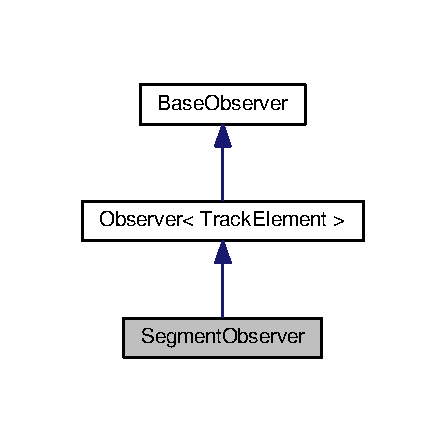
\includegraphics[width=214pt]{classKite_1_1SegmentObserver__inherit__graph}
\end{center}
\end{figure}
\subsubsection*{Public Member Functions}
\begin{DoxyCompactItemize}
\item 
virtual void \hyperlink{classKite_1_1SegmentObserver_a52e577fb0c4f2e3650928334fb621c2f}{notify} (unsigned int flags)
\end{DoxyCompactItemize}


\subsubsection{Detailed Description}
Observer on the base Auto\+Segment. 

The observer that will be hooked into the observable in the associated canonical Auto\+Segment. Used to propagate the invalidation/revalidation events from Auto\+Segment toward \hyperlink{classKite_1_1TrackSegment}{Track\+Segment}.

As a secondary function, it is used by the \hyperlink{classKite_1_1Session_a1728621b96081c32fb7bfb18a0ebfad3}{Session\+::lookup()} method to quicly retrieve \hyperlink{classKite_1_1TrackSegment}{Track\+Segment} from \textbf{ Katabatic\+::\+Auto\+Segment}. 

\subsubsection{Member Function Documentation}
\mbox{\Hypertarget{classKite_1_1SegmentObserver_a52e577fb0c4f2e3650928334fb621c2f}\label{classKite_1_1SegmentObserver_a52e577fb0c4f2e3650928334fb621c2f}} 
\index{Kite\+::\+Segment\+Observer@{Kite\+::\+Segment\+Observer}!notify@{notify}}
\index{notify@{notify}!Kite\+::\+Segment\+Observer@{Kite\+::\+Segment\+Observer}}
\paragraph{\texorpdfstring{notify()}{notify()}}
{\footnotesize\ttfamily void notify (\begin{DoxyParamCaption}\item[{unsigned int}]{flags }\end{DoxyParamCaption})\hspace{0.3cm}{\ttfamily [virtual]}}

Implement the asymmetric invalidate/revalidate policy described in \hyperlink{classKite_1_1Session}{Kite\+::\+Session}. The invalidate is immediatly passed on while the revalidate is ignored. 

Reimplemented from \textbf{ Base\+Observer}.



The documentation for this class was generated from the following files\+:\begin{DoxyCompactItemize}
\item 
Track\+Element.\+h\item 
Track\+Element.\+cpp\item 
Track\+Element.\+dox\end{DoxyCompactItemize}

\hypertarget{classKite_1_1Session}{}\subsection{Session Class Reference}
\label{classKite_1_1Session}\index{Session@{Session}}


\mbox{\hyperlink{namespaceKite}{Kite}} update \mbox{\hyperlink{classKite_1_1Session}{Session}}.  




Inheritance diagram for Session\+:\nopagebreak
\begin{figure}[H]
\begin{center}
\leavevmode
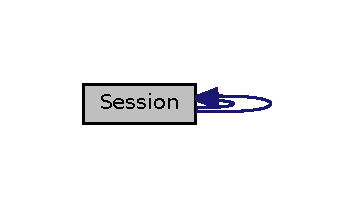
\includegraphics[width=168pt]{classKite_1_1Session__inherit__graph}
\end{center}
\end{figure}
\subsubsection*{Static Public Member Functions}
\begin{DoxyCompactItemize}
\item 
static \mbox{\hyperlink{classKite_1_1Session}{Session}} $\ast$ \mbox{\hyperlink{classKite_1_1Session_ab8362982a442b5a67f5bd76d6b6caf93}{open}} (\mbox{\hyperlink{classKite_1_1KiteEngine}{Kite\+Engine}} $\ast$)
\item 
static \mbox{\hyperlink{classKite_1_1Session}{Session}} $\ast$ \mbox{\hyperlink{classKite_1_1Session_a76f17c3642eaeba85fa0af5ae9d208b4}{get}} (const char $\ast$message=N\+U\+LL)
\item 
static \textbf{ Katabatic\+::\+Session} $\ast$ \mbox{\hyperlink{classKite_1_1Session_a8a3fc782c34dc075bb2e14209e245494}{base}} ()
\item 
static bool \mbox{\hyperlink{classKite_1_1Session_af337ffd75e4f019ce15302c60715d84b}{is\+Empty}} ()
\item 
static \mbox{\hyperlink{classKite_1_1KiteEngine}{Kite\+Engine}} $\ast$ \mbox{\hyperlink{classKite_1_1Session_a7b6c91acd2c2a7c082b3b006c1bdc91d}{get\+Kite\+Engine}} ()
\item 
static Configuration $\ast$ \mbox{\hyperlink{classKite_1_1Session_a9a7fbadfe526875680f698c76adfb128}{get\+Configuration}} ()
\item 
static \textbf{ Net} $\ast$ \mbox{\hyperlink{classKite_1_1Session_aef6f41b0e8265ad574d1797f46ab9fa8}{get\+Blockage\+Net}} ()
\item 
static \mbox{\hyperlink{classKite_1_1NegociateWindow}{Negociate\+Window}} $\ast$ \mbox{\hyperlink{classKite_1_1Session_a39ebff178f2e0abb9d5a29f485e0bbab}{get\+Negociate\+Window}} ()
\item 
static \textbf{ Katabatic\+::\+G\+Cell} $\ast$ \mbox{\hyperlink{classKite_1_1Session_a27ecb1cf5ffabe1c7901c5c894a5067d}{get\+G\+Cell\+Under}} (\textbf{ Db\+U\+::\+Unit}, \textbf{ Db\+U\+::\+Unit})
\item 
static void \mbox{\hyperlink{classKite_1_1Session_ad4f08dfb62ce626ed72023ce02e7205f}{add\+Insert\+Event}} (\mbox{\hyperlink{classKite_1_1TrackElement}{Track\+Element}} $\ast$, \mbox{\hyperlink{classKite_1_1Track}{Track}} $\ast$)
\item 
static void \mbox{\hyperlink{classKite_1_1Session_aedd573fc951ed93f8ada5b0522813c3a}{add\+Remove\+Event}} (\mbox{\hyperlink{classKite_1_1TrackElement}{Track\+Element}} $\ast$)
\item 
static void \mbox{\hyperlink{classKite_1_1Session_aa42e4cb9e2559c00d68821f535ef7838}{add\+Move\+Event}} (\mbox{\hyperlink{classKite_1_1TrackElement}{Track\+Element}} $\ast$, \mbox{\hyperlink{classKite_1_1Track}{Track}} $\ast$)
\item 
static void \mbox{\hyperlink{classKite_1_1Session_a990d32b1f1ea661b088a05f86319772f}{add\+Sort\+Event}} (\mbox{\hyperlink{classKite_1_1Track}{Track}} $\ast$, bool forced=false)
\item 
static size\+\_\+t \mbox{\hyperlink{classKite_1_1Session_a5bd93abe1416952ace15a98dbeeed124}{revalidate}} ()
\item 
static \mbox{\hyperlink{classKite_1_1TrackElement}{Track\+Element}} $\ast$ \mbox{\hyperlink{classKite_1_1Session_a1728621b96081c32fb7bfb18a0ebfad3}{lookup}} (\textbf{ Segment} $\ast$)
\item 
static \mbox{\hyperlink{classKite_1_1TrackElement}{Track\+Element}} $\ast$ \mbox{\hyperlink{classKite_1_1Session_a3946039ef19b5b6994171288f183bdaf}{lookup}} (\textbf{ Auto\+Segment} $\ast$)
\end{DoxyCompactItemize}


\subsubsection{Detailed Description}
\mbox{\hyperlink{namespaceKite}{Kite}} update \mbox{\hyperlink{classKite_1_1Session}{Session}}. 

\mbox{\hyperlink{classKite_1_1Session}{Session}} extend the Katabatic update session to the \mbox{\hyperlink{namespaceKite}{Kite}} router level. Mainly by managing \mbox{\hyperlink{classKite_1_1Track}{Track}} update.

{\bfseries Difference between \mbox{\hyperlink{namespaceKite}{Kite}} \& Katabatic sessions\+:}
\begin{DoxyItemize}
\item In Katabatic, segments are actually moved {\itshape before} the revalidation, then {\itshape during} the revalidation, contacts and topologies are adjusteds
\item In \mbox{\hyperlink{namespaceKite}{Kite}}, nothing is moved until the revalidation. Requests for segment displacement are queued for the session.
\end{DoxyItemize}

{\bfseries Asymmetry between invalidation \& revalidation\+:}
\begin{DoxyItemize}
\item When a \mbox{\hyperlink{classKite_1_1TrackSegment}{Track\+Segment}} (or directly an Auto\+Segment) is invalidated both associated Auto\+Segment and \mbox{\hyperlink{classKite_1_1TrackSegment}{Track\+Segment}} are invalidated (through the Observer mechanism).
\item When an Auto\+Segment is revalidated, the \mbox{\hyperlink{classKite_1_1TrackSegment}{Track\+Segment}} is {\bfseries not} immediatly revalidated. See the revalidate algorithm for more details.
\end{DoxyItemize}

{\bfseries Indirect \mbox{\hyperlink{classKite_1_1TrackSegment}{Track\+Segment}} invalidation\+:}
\begin{DoxyItemize}
\item \mbox{\hyperlink{classKite_1_1TrackSegment}{Track\+Segment}} invalidation do not result only from direct insertion in \mbox{\hyperlink{classKite_1_1Track}{Track}}. For example, any or all of it\textquotesingle{}s perpandicular can be invalidated trough the \textbf{ Katabatic\+::\+Session} update (the perpandicular \textbf{ Katabatic\+::\+Auto\+Segment} is revalidated, generating invalidation on their associated \mbox{\hyperlink{classKite_1_1TrackSegment}{Track\+Segment}}).
\end{DoxyItemize}

For details on how Katabatic Sessions works, have a look to \textbf{ Katabatic\+::\+Session}.\hypertarget{classKite_1_1Session_secSessionMechanism}{}\subsubsection{The Session Mechanism.}\label{classKite_1_1Session_secSessionMechanism}
Delayed modification procedure \+:
\begin{DoxyItemize}
\item Modifications events are recorded (queued) into the \mbox{\hyperlink{classKite_1_1Session}{Session}}. At this step, no modification are actually done, the data-\/base retains it\textquotesingle{}s previous state and coherency.
\item The {\ttfamily \mbox{\hyperlink{classKite_1_1Session_a5bd93abe1416952ace15a98dbeeed124}{revalidate()}}} procedure is called (or the \mbox{\hyperlink{classKite_1_1Session}{Session}} is closed), then all the modification events are applied. The data-\/base is in now in it\textquotesingle{}s new state.
\end{DoxyItemize}\hypertarget{classKite_1_1Session_secKiteSessionRevalidate}{}\subsubsection{The Revalidate Algorithm.}\label{classKite_1_1Session_secKiteSessionRevalidate}
Revalidation steps \+:
\begin{DoxyItemize}
\item Process all remove events. detach \mbox{\hyperlink{classKite_1_1TrackSegment}{Track\+Segment}} from their \mbox{\hyperlink{classKite_1_1Track}{Track}}, but do not remove the pointer from the internal {\ttfamily vector}.
\item Pack all \mbox{\hyperlink{classKite_1_1Track}{Track}} in which removal have took place.
\item Process all insert events. {\bfseries This is the time \mbox{\hyperlink{classKite_1_1TrackSegment}{Track\+Segment}} are moved into their new \mbox{\hyperlink{classKite_1_1Track}{Track}} (physical displacement)}. It is at this point that the invalidation of both Auto\+Segment and \mbox{\hyperlink{classKite_1_1TrackSegment}{Track\+Segment}} is done.
\item Call the \textbf{ Katabatic\+::\+Session\+::revalidate()} method which will recompute the correct contact extensions and topologies. {\itshape After} this step the Katabatic data-\/base is up to date, but {\itshape not} the \mbox{\hyperlink{namespaceKite}{Kite}} one. Auto\+Segment are revalidated.
\item Recompute the canonical position of source and target of all invalidateds \mbox{\hyperlink{classKite_1_1TrackSegment}{Track\+Segment}} (take account of extention modifications). The set of invalidated \mbox{\hyperlink{classKite_1_1TrackSegment}{Track\+Segment}} is computed from the revalidated Auto\+Segment, that is Auto\+Segment that are canonical.
\item Perform a sort() on all \mbox{\hyperlink{classKite_1_1Track}{Track}} that have been modifieds.
\item Now that the size of the segments have been accurately computed, look for revalidateds \mbox{\hyperlink{classKite_1_1TrackSegment}{Track\+Segment}} that\+:
\begin{DoxyEnumerate}
\item Can be reduced, generate a track remove event.
\item Must be raised, generate a routing event (put into the queue).
\end{DoxyEnumerate}
\item Process the additional track remove events.
\end{DoxyItemize}

{\bfseries Note\+:} We cannot use the Observer mechanism to automatically update \mbox{\hyperlink{classKite_1_1TrackSegment}{Track\+Segment}} from an Auto\+Segment, because we must wait for all Auto\+Segments (canonical or not) involved into the \mbox{\hyperlink{classKite_1_1TrackSegment}{Track\+Segment}} to be up to date before we can update it.

{\bfseries Note\+:} Have to talk about the special case when new canonical Auto\+Segment appears after dogleg creation.\hypertarget{classKite_1_1Session_secKiteSessionLookup}{}\subsubsection{The Lookup Mechanism}\label{classKite_1_1Session_secKiteSessionLookup}
There are two lookup mechanisms\+:
\begin{DoxyItemize}
\item From a \textbf{ Hurricane\+::\+Segment}, we uses the Katabatic segment lookup table (slow, stored in a {\ttfamily map$<$$>$}).
\item From a \textbf{ Katabatic\+::\+Auto\+Segment}, we uses the Observer, it\textquotesingle{}s owner is the \mbox{\hyperlink{classKite_1_1TrackSegment}{Track\+Segment}} (fast). 
\end{DoxyItemize}

\subsubsection{Member Function Documentation}
\mbox{\Hypertarget{classKite_1_1Session_ab8362982a442b5a67f5bd76d6b6caf93}\label{classKite_1_1Session_ab8362982a442b5a67f5bd76d6b6caf93}} 
\index{Kite\+::\+Session@{Kite\+::\+Session}!open@{open}}
\index{open@{open}!Kite\+::\+Session@{Kite\+::\+Session}}
\paragraph{\texorpdfstring{open()}{open()}}
{\footnotesize\ttfamily \mbox{\hyperlink{classKite_1_1Session}{Session}} $\ast$ open (\begin{DoxyParamCaption}\item[{\mbox{\hyperlink{classKite_1_1KiteEngine}{Kite\+Engine}} $\ast$}]{kite }\end{DoxyParamCaption})\hspace{0.3cm}{\ttfamily [static]}}


\begin{DoxyParams}{Parameters}
{\em kite} & A \mbox{\hyperlink{namespaceKite}{Kite}} Tool\+Engine on which to work. \\
\hline
\end{DoxyParams}
\begin{DoxyReturn}{Returns}
A new \mbox{\hyperlink{namespaceKite}{Kite}} update \mbox{\hyperlink{classKite_1_1Session}{Session}}.
\end{DoxyReturn}
Open a new \mbox{\hyperlink{namespaceKite}{Kite}} update \mbox{\hyperlink{classKite_1_1Session}{Session}} on the {\ttfamily kite} {\ttfamily Tool\+Engine}. At this point only one session can be opened at a time. Attempt to open a second one will result in an exception. \mbox{\Hypertarget{classKite_1_1Session_a76f17c3642eaeba85fa0af5ae9d208b4}\label{classKite_1_1Session_a76f17c3642eaeba85fa0af5ae9d208b4}} 
\index{Kite\+::\+Session@{Kite\+::\+Session}!get@{get}}
\index{get@{get}!Kite\+::\+Session@{Kite\+::\+Session}}
\paragraph{\texorpdfstring{get()}{get()}}
{\footnotesize\ttfamily \mbox{\hyperlink{classKite_1_1Session}{Session}} $\ast$ get (\begin{DoxyParamCaption}\item[{const char $\ast$}]{message = {\ttfamily NULL} }\end{DoxyParamCaption})\hspace{0.3cm}{\ttfamily [static]}}

{\bfseries Returns\+:} The currently opened session, {\ttfamily N\+U\+LL} if no session has been opened. 

Referenced by Negociate\+Window\+::run().

\mbox{\Hypertarget{classKite_1_1Session_a8a3fc782c34dc075bb2e14209e245494}\label{classKite_1_1Session_a8a3fc782c34dc075bb2e14209e245494}} 
\index{Kite\+::\+Session@{Kite\+::\+Session}!base@{base}}
\index{base@{base}!Kite\+::\+Session@{Kite\+::\+Session}}
\paragraph{\texorpdfstring{base()}{base()}}
{\footnotesize\ttfamily \textbf{ Katabatic\+::\+Session} $\ast$ base (\begin{DoxyParamCaption}{ }\end{DoxyParamCaption})\hspace{0.3cm}{\ttfamily [inline]}, {\ttfamily [static]}}

{\bfseries Returns\+:} The \mbox{\hyperlink{classKite_1_1Session}{Session}}, casted as it\textquotesingle{}s base object. \mbox{\Hypertarget{classKite_1_1Session_af337ffd75e4f019ce15302c60715d84b}\label{classKite_1_1Session_af337ffd75e4f019ce15302c60715d84b}} 
\index{Kite\+::\+Session@{Kite\+::\+Session}!is\+Empty@{is\+Empty}}
\index{is\+Empty@{is\+Empty}!Kite\+::\+Session@{Kite\+::\+Session}}
\paragraph{\texorpdfstring{is\+Empty()}{isEmpty()}}
{\footnotesize\ttfamily bool is\+Empty (\begin{DoxyParamCaption}{ }\end{DoxyParamCaption})\hspace{0.3cm}{\ttfamily [inline]}, {\ttfamily [static]}}

Ensure that the \mbox{\hyperlink{classKite_1_1Session}{Session}} is empty and can be closed (deleted) safely. 

Referenced by Negociate\+Window\+::run().

\mbox{\Hypertarget{classKite_1_1Session_a7b6c91acd2c2a7c082b3b006c1bdc91d}\label{classKite_1_1Session_a7b6c91acd2c2a7c082b3b006c1bdc91d}} 
\index{Kite\+::\+Session@{Kite\+::\+Session}!get\+Kite\+Engine@{get\+Kite\+Engine}}
\index{get\+Kite\+Engine@{get\+Kite\+Engine}!Kite\+::\+Session@{Kite\+::\+Session}}
\paragraph{\texorpdfstring{get\+Kite\+Engine()}{getKiteEngine()}}
{\footnotesize\ttfamily \mbox{\hyperlink{classKite_1_1KiteEngine}{Kite\+Engine}} $\ast$ get\+Kite\+Engine (\begin{DoxyParamCaption}{ }\end{DoxyParamCaption})\hspace{0.3cm}{\ttfamily [inline]}, {\ttfamily [static]}}

{\bfseries Returns\+:} The \mbox{\hyperlink{namespaceKite}{Kite}} Tool\+Engine associated to the current update session (proxy helper). 

Referenced by Manipulator\+::can\+Ripup(), Segment\+Fsm\+::conflict\+Solve\+By\+History(), Segment\+Fsm\+::conflict\+Solve\+By\+Placeds(), Negociate\+Window\+::create\+Track\+Segment(), Segment\+Action\+::do\+Action(), Routing\+Event\+::process(), Routing\+Event\+::revalidate(), Manipulator\+::ripple(), Manipulator\+::ripup\+Perpandiculars(), Negociate\+Window\+::run(), Segment\+Fsm\+::\+Segment\+Fsm(), and Negociate\+Window\+::set\+G\+Cells().

\mbox{\Hypertarget{classKite_1_1Session_a9a7fbadfe526875680f698c76adfb128}\label{classKite_1_1Session_a9a7fbadfe526875680f698c76adfb128}} 
\index{Kite\+::\+Session@{Kite\+::\+Session}!get\+Configuration@{get\+Configuration}}
\index{get\+Configuration@{get\+Configuration}!Kite\+::\+Session@{Kite\+::\+Session}}
\paragraph{\texorpdfstring{get\+Configuration()}{getConfiguration()}}
{\footnotesize\ttfamily Configuration $\ast$ get\+Configuration (\begin{DoxyParamCaption}{ }\end{DoxyParamCaption})\hspace{0.3cm}{\ttfamily [static]}}

{\bfseries Returns\+:} The \mbox{\hyperlink{namespaceKite}{Kite}} Configuration of the Router (proxy helper). \mbox{\Hypertarget{classKite_1_1Session_aef6f41b0e8265ad574d1797f46ab9fa8}\label{classKite_1_1Session_aef6f41b0e8265ad574d1797f46ab9fa8}} 
\index{Kite\+::\+Session@{Kite\+::\+Session}!get\+Blockage\+Net@{get\+Blockage\+Net}}
\index{get\+Blockage\+Net@{get\+Blockage\+Net}!Kite\+::\+Session@{Kite\+::\+Session}}
\paragraph{\texorpdfstring{get\+Blockage\+Net()}{getBlockageNet()}}
{\footnotesize\ttfamily \textbf{ Net} $\ast$ get\+Blockage\+Net (\begin{DoxyParamCaption}{ }\end{DoxyParamCaption})\hspace{0.3cm}{\ttfamily [inline]}, {\ttfamily [static]}}

{\bfseries Returns\+:} The net used to create blockage components (proxy helper). 

Referenced by Track\+Fixed\+Segment\+::create().

\mbox{\Hypertarget{classKite_1_1Session_a39ebff178f2e0abb9d5a29f485e0bbab}\label{classKite_1_1Session_a39ebff178f2e0abb9d5a29f485e0bbab}} 
\index{Kite\+::\+Session@{Kite\+::\+Session}!get\+Negociate\+Window@{get\+Negociate\+Window}}
\index{get\+Negociate\+Window@{get\+Negociate\+Window}!Kite\+::\+Session@{Kite\+::\+Session}}
\paragraph{\texorpdfstring{get\+Negociate\+Window()}{getNegociateWindow()}}
{\footnotesize\ttfamily \mbox{\hyperlink{classKite_1_1NegociateWindow}{Negociate\+Window}} $\ast$ get\+Negociate\+Window (\begin{DoxyParamCaption}{ }\end{DoxyParamCaption})\hspace{0.3cm}{\ttfamily [inline]}, {\ttfamily [static]}}

{\bfseries Returns\+:} The current \mbox{\hyperlink{classKite_1_1NegociateWindow}{Negociate\+Window}} (proxy helper). 

Referenced by Track\+Segment\+::\+\_\+post\+Doglegs(), and Track\+Segment\+::reschedule().

\mbox{\Hypertarget{classKite_1_1Session_a27ecb1cf5ffabe1c7901c5c894a5067d}\label{classKite_1_1Session_a27ecb1cf5ffabe1c7901c5c894a5067d}} 
\index{Kite\+::\+Session@{Kite\+::\+Session}!get\+G\+Cell\+Under@{get\+G\+Cell\+Under}}
\index{get\+G\+Cell\+Under@{get\+G\+Cell\+Under}!Kite\+::\+Session@{Kite\+::\+Session}}
\paragraph{\texorpdfstring{get\+G\+Cell\+Under()}{getGCellUnder()}}
{\footnotesize\ttfamily \textbf{ Katabatic\+::\+G\+Cell} $\ast$ get\+G\+Cell\+Under (\begin{DoxyParamCaption}\item[{\textbf{ Db\+U\+::\+Unit}}]{x,  }\item[{\textbf{ Db\+U\+::\+Unit}}]{y }\end{DoxyParamCaption})\hspace{0.3cm}{\ttfamily [inline]}, {\ttfamily [static]}}

{\bfseries Returns\+:} The G\+Cell under {\ttfamily }(x,y) (proxy helper, see \textbf{ Katabatic\+::\+G\+Cell\+Grid\+::get\+G\+Cell()}). 

Referenced by Segment\+Fsm\+::conflict\+Solve\+By\+History().

\mbox{\Hypertarget{classKite_1_1Session_ad4f08dfb62ce626ed72023ce02e7205f}\label{classKite_1_1Session_ad4f08dfb62ce626ed72023ce02e7205f}} 
\index{Kite\+::\+Session@{Kite\+::\+Session}!add\+Insert\+Event@{add\+Insert\+Event}}
\index{add\+Insert\+Event@{add\+Insert\+Event}!Kite\+::\+Session@{Kite\+::\+Session}}
\paragraph{\texorpdfstring{add\+Insert\+Event()}{addInsertEvent()}}
{\footnotesize\ttfamily void add\+Insert\+Event (\begin{DoxyParamCaption}\item[{\mbox{\hyperlink{classKite_1_1TrackElement}{Track\+Element}} $\ast$}]{segment,  }\item[{\mbox{\hyperlink{classKite_1_1Track}{Track}} $\ast$}]{track }\end{DoxyParamCaption})\hspace{0.3cm}{\ttfamily [inline]}, {\ttfamily [static]}}


\begin{DoxyParams}{Parameters}
{\em segment} & An Auto\+Segment to insert in a \mbox{\hyperlink{classKite_1_1Track}{Track}}. \\
\hline
{\em track} & The \mbox{\hyperlink{classKite_1_1Track}{Track}} into which the {\itshape segment} will be inserted.\\
\hline
\end{DoxyParams}
Schedule the insertion of {\itshape segment} into \mbox{\hyperlink{classKite_1_1Track}{Track}} {\itshape track}. The {\itshape segment} must not already be part of a \mbox{\hyperlink{classKite_1_1Track}{Track}}. \mbox{\Hypertarget{classKite_1_1Session_aedd573fc951ed93f8ada5b0522813c3a}\label{classKite_1_1Session_aedd573fc951ed93f8ada5b0522813c3a}} 
\index{Kite\+::\+Session@{Kite\+::\+Session}!add\+Remove\+Event@{add\+Remove\+Event}}
\index{add\+Remove\+Event@{add\+Remove\+Event}!Kite\+::\+Session@{Kite\+::\+Session}}
\paragraph{\texorpdfstring{add\+Remove\+Event()}{addRemoveEvent()}}
{\footnotesize\ttfamily void add\+Remove\+Event (\begin{DoxyParamCaption}\item[{\mbox{\hyperlink{classKite_1_1TrackElement}{Track\+Element}} $\ast$}]{segment }\end{DoxyParamCaption})\hspace{0.3cm}{\ttfamily [inline]}, {\ttfamily [static]}}


\begin{DoxyParams}{Parameters}
{\em segment} & A \mbox{\hyperlink{classKite_1_1TrackSegment}{Track\+Segment}} to remove from a \mbox{\hyperlink{classKite_1_1Track}{Track}}.\\
\hline
\end{DoxyParams}
Schedule the removal of {\itshape segment} from \mbox{\hyperlink{classKite_1_1Track}{Track}} {\itshape track}. 

Referenced by Segment\+Action\+::do\+Action(), and Track\+Segment\+::reschedule().

\mbox{\Hypertarget{classKite_1_1Session_aa42e4cb9e2559c00d68821f535ef7838}\label{classKite_1_1Session_aa42e4cb9e2559c00d68821f535ef7838}} 
\index{Kite\+::\+Session@{Kite\+::\+Session}!add\+Move\+Event@{add\+Move\+Event}}
\index{add\+Move\+Event@{add\+Move\+Event}!Kite\+::\+Session@{Kite\+::\+Session}}
\paragraph{\texorpdfstring{add\+Move\+Event()}{addMoveEvent()}}
{\footnotesize\ttfamily void add\+Move\+Event (\begin{DoxyParamCaption}\item[{\mbox{\hyperlink{classKite_1_1TrackElement}{Track\+Element}} $\ast$}]{segment,  }\item[{\mbox{\hyperlink{classKite_1_1Track}{Track}} $\ast$}]{track }\end{DoxyParamCaption})\hspace{0.3cm}{\ttfamily [inline]}, {\ttfamily [static]}}


\begin{DoxyParams}{Parameters}
{\em segment} & An Auto\+Segment to move into a new \mbox{\hyperlink{classKite_1_1Track}{Track}}. \\
\hline
{\em track} & The \mbox{\hyperlink{classKite_1_1Track}{Track}} into which the {\itshape segment} will be moved.\\
\hline
\end{DoxyParams}
Schedule the displacement of {\itshape segment} into \mbox{\hyperlink{classKite_1_1Track}{Track}} {\itshape track}. \mbox{\Hypertarget{classKite_1_1Session_a990d32b1f1ea661b088a05f86319772f}\label{classKite_1_1Session_a990d32b1f1ea661b088a05f86319772f}} 
\index{Kite\+::\+Session@{Kite\+::\+Session}!add\+Sort\+Event@{add\+Sort\+Event}}
\index{add\+Sort\+Event@{add\+Sort\+Event}!Kite\+::\+Session@{Kite\+::\+Session}}
\paragraph{\texorpdfstring{add\+Sort\+Event()}{addSortEvent()}}
{\footnotesize\ttfamily void add\+Sort\+Event (\begin{DoxyParamCaption}\item[{\mbox{\hyperlink{classKite_1_1Track}{Track}} $\ast$}]{track,  }\item[{bool}]{forced = {\ttfamily false} }\end{DoxyParamCaption})\hspace{0.3cm}{\ttfamily [inline]}, {\ttfamily [static]}}


\begin{DoxyParams}{Parameters}
{\em track} & The \mbox{\hyperlink{classKite_1_1Track}{Track}} to update. \\
\hline
{\em forced} & Force the invalidation of the {\ttfamily \mbox{\hyperlink{classKite_1_1Track}{Track}}}.\\
\hline
\end{DoxyParams}
Schedule the update of \mbox{\hyperlink{classKite_1_1Track}{Track}} {\itshape track}. If the {\ttfamily \mbox{\hyperlink{classKite_1_1Track}{Track}}} has not been invalidated, no actual sort will takes place. To force a sort (manually invalidating the {\ttfamily \mbox{\hyperlink{classKite_1_1Track}{Track}}}), sets {\bfseries forced} to {\bfseries true}.

{\bfseries See also\+:}~ Track\+::pack() \& Track\+::sort(). 

Referenced by Track\+Segment\+::revalidate().

\mbox{\Hypertarget{classKite_1_1Session_a5bd93abe1416952ace15a98dbeeed124}\label{classKite_1_1Session_a5bd93abe1416952ace15a98dbeeed124}} 
\index{Kite\+::\+Session@{Kite\+::\+Session}!revalidate@{revalidate}}
\index{revalidate@{revalidate}!Kite\+::\+Session@{Kite\+::\+Session}}
\paragraph{\texorpdfstring{revalidate()}{revalidate()}}
{\footnotesize\ttfamily void revalidate (\begin{DoxyParamCaption}{ }\end{DoxyParamCaption})\hspace{0.3cm}{\ttfamily [inline]}, {\ttfamily [static]}}

Applies all the requested modifications, but keeping the session opened. 

Referenced by Routing\+Event\+::process(), Negociate\+Window\+::run(), and Negociate\+Window\+::set\+G\+Cells().

\mbox{\Hypertarget{classKite_1_1Session_a1728621b96081c32fb7bfb18a0ebfad3}\label{classKite_1_1Session_a1728621b96081c32fb7bfb18a0ebfad3}} 
\index{Kite\+::\+Session@{Kite\+::\+Session}!lookup@{lookup}}
\index{lookup@{lookup}!Kite\+::\+Session@{Kite\+::\+Session}}
\paragraph{\texorpdfstring{lookup()}{lookup()}\hspace{0.1cm}{\footnotesize\ttfamily [1/2]}}
{\footnotesize\ttfamily \mbox{\hyperlink{classKite_1_1TrackElement}{Track\+Element}} $\ast$ lookup (\begin{DoxyParamCaption}\item[{\textbf{ Segment} $\ast$}]{segment }\end{DoxyParamCaption})\hspace{0.3cm}{\ttfamily [static]}}

{\bfseries Returns\+:} the \mbox{\hyperlink{classKite_1_1TrackElement}{Track\+Element}} associated to {\ttfamily segment}. 

Referenced by Negociate\+Window\+::compute\+Wirelength(), Track\+Segment\+::create(), Track\+Segment\+::get\+Canonical(), Track\+Segment\+::get\+Parent(), Track\+Segment\+::get\+Source\+Dogleg(), Track\+Segment\+::get\+Target\+Dogleg(), Manipulator\+::relax(), Routing\+Event\+Queue\+::repush\+Invalidateds(), and Negociate\+Window\+::set\+G\+Cells().

\mbox{\Hypertarget{classKite_1_1Session_a3946039ef19b5b6994171288f183bdaf}\label{classKite_1_1Session_a3946039ef19b5b6994171288f183bdaf}} 
\index{Kite\+::\+Session@{Kite\+::\+Session}!lookup@{lookup}}
\index{lookup@{lookup}!Kite\+::\+Session@{Kite\+::\+Session}}
\paragraph{\texorpdfstring{lookup()}{lookup()}\hspace{0.1cm}{\footnotesize\ttfamily [2/2]}}
{\footnotesize\ttfamily \mbox{\hyperlink{classKite_1_1TrackElement}{Track\+Element}} $\ast$ lookup (\begin{DoxyParamCaption}\item[{\textbf{ Auto\+Segment} $\ast$}]{segment }\end{DoxyParamCaption})\hspace{0.3cm}{\ttfamily [static]}}

{\bfseries Returns\+:} the \mbox{\hyperlink{classKite_1_1TrackElement}{Track\+Element}} associated to {\ttfamily segment}. 

The documentation for this class was generated from the following files\+:\begin{DoxyCompactItemize}
\item 
Session.\+h\item 
Session.\+dox\end{DoxyCompactItemize}

\hypertarget{classKite_1_1Track}{\subsection{Track Class Reference}
\label{classKite_1_1Track}\index{Track@{Track}}
}


Structure managing one routing track.  




Inheritance diagram for Track\-:\nopagebreak
\begin{figure}[H]
\begin{center}
\leavevmode
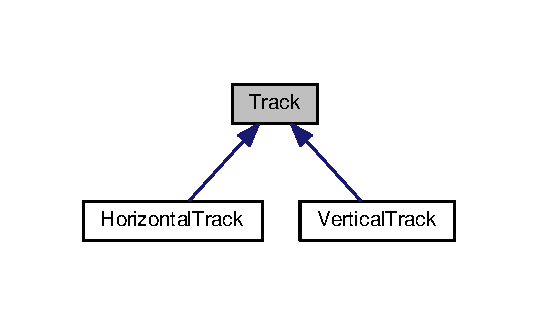
\includegraphics[width=258pt]{classKite_1_1Track__inherit__graph}
\end{center}
\end{figure}
\subsubsection*{Public Types}
\begin{DoxyCompactItemize}
\item 
enum \hyperlink{classKite_1_1Track_af4bdc8469c0fee386fc2ff30e0666bca}{Index\-State} \{ \\*
\hyperlink{classKite_1_1Track_af4bdc8469c0fee386fc2ff30e0666bcaa8b61f6a736a067f2124ee5bd5cb8ac71}{Begin\-Is\-Track\-Min} = 0x00000001, 
\\*
\hyperlink{classKite_1_1Track_af4bdc8469c0fee386fc2ff30e0666bcaa2558894ee6c661f4c13276cc8f2464a4}{Begin\-Is\-Segment\-Min} = 0x00000002, 
\\*
\hyperlink{classKite_1_1Track_af4bdc8469c0fee386fc2ff30e0666bcaa8b6241764173838bf07e69fb78b688a4}{Begin\-Is\-Segment\-Max} = 0x00000004, 
\\*
\hyperlink{classKite_1_1Track_af4bdc8469c0fee386fc2ff30e0666bcaa405dc0d4b2391506d0dcc4a75d5f1ba2}{End\-Is\-Track\-Max} = 0x00000008, 
\\*
\hyperlink{classKite_1_1Track_af4bdc8469c0fee386fc2ff30e0666bcaa24e6a845af9d42451a2c41f2f8d388d1}{End\-Is\-Segment\-Min} = 0x00000010, 
\\*
\hyperlink{classKite_1_1Track_af4bdc8469c0fee386fc2ff30e0666bcaa03aebc159f233b883124bd19fdd2ea0f}{End\-Is\-Next\-Segment\-Min} = 0x00000020, 
\\*
\hyperlink{classKite_1_1Track_af4bdc8469c0fee386fc2ff30e0666bcaab507ecf157f576817fafc5e7deb71629}{End\-Is\-Segment\-Max} = 0x00000040, 
\\*
\hyperlink{classKite_1_1Track_af4bdc8469c0fee386fc2ff30e0666bcaa5c7f72d6942ae38d66f530bea1063adf}{Before\-First\-Element} = Begin\-Is\-Track\-Min $|$\-End\-Is\-Segment\-Min, 
\\*
\hyperlink{classKite_1_1Track_af4bdc8469c0fee386fc2ff30e0666bcaa36e625d718c74f5ff503638360ba1166}{Inside\-Element} = Begin\-Is\-Segment\-Min$|$\-End\-Is\-Segment\-Max, 
\\*
\hyperlink{classKite_1_1Track_af4bdc8469c0fee386fc2ff30e0666bcaa55d08f66f21334eb8c0dca170f1cb8a4}{Outside\-Element} = Begin\-Is\-Segment\-Max$|$\-End\-Is\-Next\-Segment\-Min, 
\\*
\hyperlink{classKite_1_1Track_af4bdc8469c0fee386fc2ff30e0666bcaa3fc579452c9779cd2865d5019a61c6a5}{After\-Last\-Element} = Begin\-Is\-Segment\-Max$|$\-End\-Is\-Track\-Max, 
\\*
\hyperlink{classKite_1_1Track_af4bdc8469c0fee386fc2ff30e0666bcaaa697b71e325cea0980e9555654f8f3cf}{Empty\-Track} = Begin\-Is\-Track\-Min $|$\-End\-Is\-Track\-Max, 
\\*
\hyperlink{classKite_1_1Track_af4bdc8469c0fee386fc2ff30e0666bcaa8621fa6a5b7a491fd1bf8dd7f0dd3589}{Begin\-Mask} = Begin\-Is\-Track\-Min $|$\-Begin\-Is\-Segment\-Min$|$\-Begin\-Is\-Segment\-Max, 
\\*
\hyperlink{classKite_1_1Track_af4bdc8469c0fee386fc2ff30e0666bcaa0b5a81972d3a6718c3d68199467d2d11}{End\-Mask} = End\-Is\-Track\-Max $|$\-End\-Is\-Segment\-Min $|$\-End\-Is\-Next\-Segment\-Min$|$\-End\-Is\-Segment\-Max
 \}
\end{DoxyCompactItemize}
\subsubsection*{Public Member Functions}
\begin{DoxyCompactItemize}
\item 
virtual bool \hyperlink{classKite_1_1Track_a9d3db1f8a5aca58f8f54d291faebf873}{is\-Horizontal} () const =0
\item 
virtual bool \hyperlink{classKite_1_1Track_a6fa2bf0568a2b295dd7cd1f7207247d5}{is\-Vertical} () const =0
\item 
bool \hyperlink{classKite_1_1Track_ac9f5f43a21bc7b63a1237e10b5a6a53b}{is\-Local\-Assigned} () const 
\item 
\hyperlink{classKite_1_1RoutingPlane}{Routing\-Plane} $\ast$ \hyperlink{classKite_1_1Track_a3f7a5bbb3140598c747b1526998e6be7}{get\-Routing\-Plane} () const 
\item 
\hyperlink{classKite_1_1KiteEngine}{Kite\-Engine} $\ast$ \hyperlink{classKite_1_1Track_a9ccc00efc7079210bc25122921382da4}{get\-Kite\-Engine} () const 
\item 
virtual unsigned int \hyperlink{classKite_1_1Track_ae35b78590ed6aa546b626ef95f28c533}{get\-Direction} () const =0
\item 
size\-\_\-t \hyperlink{classKite_1_1Track_a65742a66b3c3b66d5b619db492469900}{get\-Index} () const 
\item 
unsigned int \hyperlink{classKite_1_1Track_ad43be8bb2a3c8247405feef4fa973734}{get\-Depth} () const 
\item 
const {\bf Layer} $\ast$ \hyperlink{classKite_1_1Track_ac1bbd63624eb1b4e394301c92adef62c}{get\-Layer} () const 
\item 
const {\bf Layer} $\ast$ \hyperlink{classKite_1_1Track_aceadd4784a0ae6394d2c75433f81ce59}{get\-Blockage\-Layer} () const 
\item 
{\bf Db\-U\-::\-Unit} \hyperlink{classKite_1_1Track_af85576c58c70007850ad56e238e8d266}{get\-Axis} () const 
\item 
{\bf Db\-U\-::\-Unit} \hyperlink{classKite_1_1Track_a75e87715af5a758c37e5f1faeaf7ccc1}{get\-Min} () const 
\item 
{\bf Db\-U\-::\-Unit} \hyperlink{classKite_1_1Track_a204f3392bd6abab056796ecdae72ce54}{get\-Max} () const 
\item 
\hyperlink{classKite_1_1Track}{Track} $\ast$ \hyperlink{classKite_1_1Track_ab83ae7101fae68a7db48b96a82cc42f5}{get\-Next\-Track} () const 
\item 
\hyperlink{classKite_1_1Track}{Track} $\ast$ \hyperlink{classKite_1_1Track_a0647664eabb2f70005585316c3681b7f}{get\-Previous\-Track} () const 
\item 
size\-\_\-t \hyperlink{classKite_1_1Track_af55b3790622878d65ed5ff2bb2b3fcc4}{get\-Size} () const 
\item 
virtual {\bf Point} \hyperlink{classKite_1_1Track_a2a033f90e528d3d07aa33694dd733200}{get\-Position} ({\bf Db\-U\-::\-Unit} coordinate) const =0
\item 
\hyperlink{classKite_1_1TrackElement}{Track\-Element} $\ast$ \hyperlink{classKite_1_1Track_ac2216be50494af61a7b16d20dd8cc5dd}{get\-Segment} (size\-\_\-t index) const 
\item 
\hyperlink{classKite_1_1TrackElement}{Track\-Element} $\ast$ \hyperlink{classKite_1_1Track_aa8a5a7f28e71bce3676d4a051ab1d6c6}{get\-Segment} ({\bf Db\-U\-::\-Unit} position) const 
\item 
\hyperlink{classKite_1_1TrackElement}{Track\-Element} $\ast$ \hyperlink{classKite_1_1Track_afaad0c947c459bab3b7ef742aaa5c59f}{get\-Next} (size\-\_\-t \&index, {\bf Net} $\ast$) const 
\item 
\hyperlink{classKite_1_1TrackElement}{Track\-Element} $\ast$ \hyperlink{classKite_1_1Track_a4ebcb68fdea325b48de96a417a86d896}{get\-Previous} (size\-\_\-t \&index, {\bf Net} $\ast$) const 
\item 
\hyperlink{classKite_1_1TrackElement}{Track\-Element} $\ast$ \hyperlink{classKite_1_1Track_a13493827f36a960f3c443ff2b8ea0143}{get\-Next\-Fixed} (size\-\_\-t \&index) const 
\item 
size\-\_\-t \hyperlink{classKite_1_1Track_a92159b77cb6e17d1c81fe6b907953387}{find} (const \hyperlink{classKite_1_1TrackElement}{Track\-Element} $\ast$) const 
\item 
{\bf Db\-U\-::\-Unit} \hyperlink{classKite_1_1Track_a67e86dd6909fb12706787ea738355fdf}{get\-Source\-Position} (vector$<$ \hyperlink{classKite_1_1TrackElement}{Track\-Element} $\ast$ $>$\-::iterator) const 
\item 
{\bf Db\-U\-::\-Unit} \hyperlink{classKite_1_1Track_a00032371424630b4fd99dc1c443ee1f3}{get\-Minimal\-Position} (size\-\_\-t index, unsigned int state) const 
\item 
{\bf Db\-U\-::\-Unit} \hyperlink{classKite_1_1Track_a5c9424f73f1fafa422c8dca99c7216bd}{get\-Maximal\-Position} (size\-\_\-t index, unsigned int state) const 
\item 
{\bf Interval} \hyperlink{classKite_1_1Track_a95a9fad401e395a6b0f73e755db6ddad}{get\-Free\-Interval} ({\bf Db\-U\-::\-Unit} position, {\bf Net} $\ast$net=N\-U\-L\-L) const 
\item 
{\bf Interval} \hyperlink{classKite_1_1Track_aeb4b9c2a20ec5f82da8781b11982ae7d}{get\-Occupied\-Interval} (size\-\_\-t \&begin) const 
\item 
{\bf Interval} \hyperlink{classKite_1_1Track_aead0aa746d8c8ce14a11161baa1aafc4}{expand\-Free\-Interval} (size\-\_\-t \&begin, size\-\_\-t \&end, unsigned int state, {\bf Net} $\ast$) const 
\item 
void \hyperlink{classKite_1_1Track_a7386d7acfcd1dfbeb906bd4c482d797e}{get\-Begin\-Index} ({\bf Db\-U\-::\-Unit} position, size\-\_\-t \&begin, unsigned int \&state) const 
\item 
void \hyperlink{classKite_1_1Track_a414e800da5aa8b03eb82aa0dba883f7f}{get\-Overlap\-Bounds} ({\bf Interval}, size\-\_\-t \&begin, size\-\_\-t \&end) const 
\item 
Track\-Cost \hyperlink{classKite_1_1Track_a91b5c29bec3f74b1194473d1eb274086}{get\-Overlap\-Cost} ({\bf Interval}, {\bf Net} $\ast$, size\-\_\-t begin, size\-\_\-t end, unsigned int flags) const 
\item 
Track\-Cost \hyperlink{classKite_1_1Track_ae8e0a72955bd05677d82738ad032526d}{get\-Overlap\-Cost} ({\bf Interval}, {\bf Net} $\ast$, unsigned int flags) const 
\item 
Track\-Cost \hyperlink{classKite_1_1Track_ac930c18bbcb0b25f2b5360f6ce6741e7}{get\-Overlap\-Cost} (\hyperlink{classKite_1_1TrackElement}{Track\-Element} $\ast$, unsigned int flags) const 
\item 
void \hyperlink{classKite_1_1Track_a8b274bcf60589230f36f9798cce1e7d7}{get\-Terminal\-Weight} ({\bf Interval}, {\bf Net} $\ast$, size\-\_\-t \&count, unsigned int \&weight) const 
\item 
{\bf Db\-U\-::\-Unit} \hyperlink{classKite_1_1Track_a6807aafaa83c1a2687c48d02510ced3a}{get\-Source\-Position} (size\-\_\-t index) const 
\item 
bool \hyperlink{classKite_1_1Track_ad21778972fbdf5cbffb470b2e36f9fcf}{check} (unsigned int \&overlaps, const char $\ast$message=N\-U\-L\-L) const 
\item 
void \hyperlink{classKite_1_1Track_a893f1101c650c08c98612515c2b1a89c}{invalidate} ()
\item 
void \hyperlink{classKite_1_1Track_aa392ba7cf1e3e485aac11cf326e31918}{insert} (\hyperlink{classKite_1_1TrackElement}{Track\-Element} $\ast$)
\item 
void \hyperlink{classKite_1_1Track_a31e8f4502866435ac898c7eec741175f}{insert} (\hyperlink{classKite_1_1TrackMarker}{Track\-Marker} $\ast$)
\item 
void \hyperlink{classKite_1_1Track_a8b5d93406ef581c1be022417238a89ca}{set\-Segment} (\hyperlink{classKite_1_1TrackElement}{Track\-Element} $\ast$, size\-\_\-t)
\item 
size\-\_\-t \hyperlink{classKite_1_1Track_abfffcd781865b94f62f27a1e7be99a38}{do\-Removal} ()
\item 
void \hyperlink{classKite_1_1Track_aaccb9224f5b38ecd8506fd1eec9ef5ca}{do\-Reorder} ()
\end{DoxyCompactItemize}
\subsubsection*{Static Public Attributes}
\begin{DoxyCompactItemize}
\item 
static const size\-\_\-t \hyperlink{classKite_1_1Track_ae0070ea45b2592ce3701ab9e486e58a0}{npos} = (size\-\_\-t)-\/1
\end{DoxyCompactItemize}


\subsubsection{Detailed Description}
Structure managing one routing track. 

\hypertarget{classKite_1_1Track_secTrackPurpose}{}\subsubsection{Track Purpose}\label{classKite_1_1Track_secTrackPurpose}
We use an array of {\itshape regularly spaced} \hyperlink{classKite_1_1Track}{Track} as a geometrical fast access structure. It allows to know whether an area is used or not. The whole area may be seen as a set of adjoining tiles of fixed {\itshape width} but variable {\itshape length}.

The figure {\bfseries (1.\-b)} show, for an horizontal, track the relation between {\ttfamily y,min,max} and the occupied area of the plane. {\ttfamily min} and {\ttfamily max} must take into account segment extensions ({\ttfamily e}) and the minimal distance between two rectangles ({\ttfamily M\-D}) of the same layer. We assume that the width of the segment, augmented of all it's contraints is no greater than {\ttfamily T\-S} (in fact it's how {\ttfamily T\-S} must be calculated).

For the whole track array, see \hyperlink{classKite_1_1RoutingPlane}{Routing\-Plane}.

\hypertarget{classKite_1_1Track_secTrackImplementation}{}\subsubsection{Track Implementation}\label{classKite_1_1Track_secTrackImplementation}
A \hyperlink{classKite_1_1Track}{Track} is implemented with a sorted vector of \hyperlink{classKite_1_1TrackElement}{Track\-Element}. Track\-Elements from differents nets must not overlap. The sorting order is defined as follow\-:
\begin{DoxyItemize}
\item Track\-Elements are sorted by increasing source ({\itshape min}) positions.
\item In case of overlap (i.\-e. belongs to the same net), if they share the same source position, then they are sorted by {\itshape decreasing} length. This way, the longest one will be the first encountered when walking through the \hyperlink{classKite_1_1Track}{Track} in increasing index order.
\end{DoxyItemize}

Figure {\bfseries 2.\-b} shows the details of the \hyperlink{classKite_1_1Track}{Track} {\bfseries \mbox{[}1\mbox{]}} of figure {\bfseries 1.\-a}. Net {\bfseries $<$d$>$} show an exemple of overlapping.

 
\begin{DoxyImage}
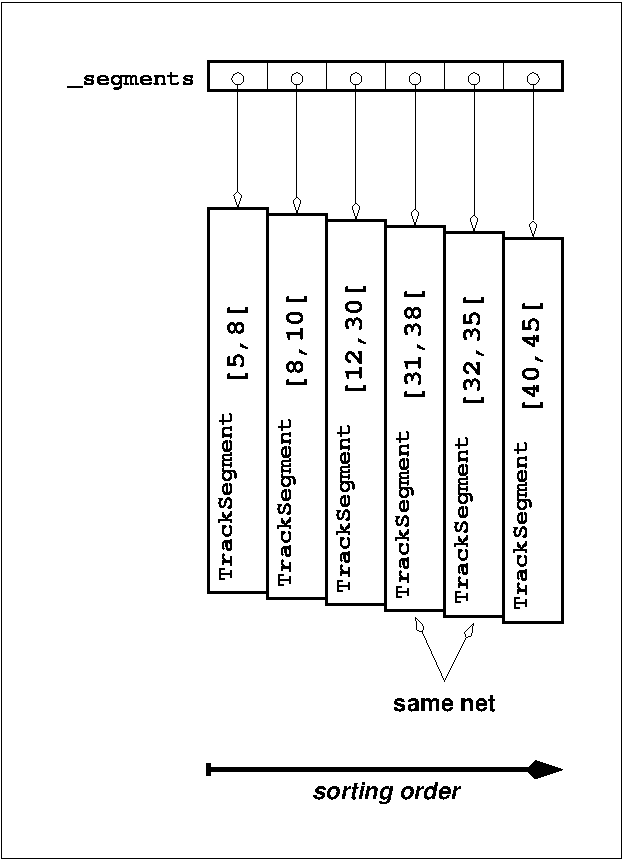
\includegraphics[width=0.7\textwidth]{Track-1}
\caption{Track Structure}
\end{DoxyImage}


In addition to the Track\-Segments, the \hyperlink{classKite_1_1Track}{Track} also manage additionnal informations through a second vector of Track\-Markers. \hyperlink{classKite_1_1TrackMarker}{Track\-Marker} are currently used only to hints at how strongly a terminal is dependant on that portion of \hyperlink{classKite_1_1Track}{Track} to be accessed.\hypertarget{classKite_1_1Track_ssecTrackIndexes}{}\paragraph{Indexes vs. Iterators}\label{classKite_1_1Track_ssecTrackIndexes}
Numerical indexes have been prefered over iterators because they can be used more easily by objects other the \hyperlink{classKite_1_1Track}{Track} itself for referencing. So internal managment follow the same rule, handling indexes or reference to indexes.\hypertarget{classKite_1_1Track_ssecTrackUpdate}{}\paragraph{Update Mechanism}\label{classKite_1_1Track_ssecTrackUpdate}
When a \hyperlink{classKite_1_1TrackElement}{Track\-Element} is normaly inserted in a \hyperlink{classKite_1_1Track}{Track}, a two way link is established. The \hyperlink{classKite_1_1Track}{Track} has an entry in it's vector refering to \hyperlink{classKite_1_1TrackElement}{Track\-Element}, and conversely, the \hyperlink{classKite_1_1TrackElement}{Track\-Element} has it's {\ttfamily track} field pointing to it's owning \hyperlink{classKite_1_1Track}{Track}.

{\bfseries \hyperlink{classKite_1_1TrackElement}{Track\-Element} Removal}

To remove a \hyperlink{classKite_1_1TrackElement}{Track\-Element} from a \hyperlink{classKite_1_1Track}{Track}, we break one of those two links\-: the \hyperlink{classKite_1_1TrackElement}{Track\-Element} cease to refer to the owning \hyperlink{classKite_1_1Track}{Track}, marking him for removal which will occurs at the next track revalidation (\hyperlink{classKite_1_1Track_abfffcd781865b94f62f27a1e7be99a38}{Track\-::do\-Removal()}). In figure {\bfseries 3}, the \hyperlink{classKite_1_1TrackElement}{Track\-Element} belonging to net {\bfseries $<$b$>$} is marked for removal.

 {\bfseries \hyperlink{classKite_1_1TrackElement}{Track\-Element} Insertion}

When a \hyperlink{classKite_1_1TrackElement}{Track\-Element} is inserted into a \hyperlink{classKite_1_1Track}{Track}, the two way link is immediatly created (but the \hyperlink{classKite_1_1TrackElement}{Track\-Element} is not yet at it's final place in the \hyperlink{classKite_1_1Track}{Track}'s vector). Before inserting a \hyperlink{classKite_1_1TrackElement}{Track\-Element} we check that it's been already detached ({\ttfamily track} field to {\ttfamily N\-U\-L\-L}).

It is at that step that the \hyperlink{classKite_1_1TrackElement}{Track\-Element} axis is actually updated through a call to \hyperlink{classKite_1_1TrackElement_a45e685b1e3ee630d24bf43746553af4c}{Track\-Element\-::set\-Axis()}.

{\bfseries Revalidation Sequence}

After a \hyperlink{classKite_1_1Track}{Track} has been modificated either the \hyperlink{classKite_1_1Track}{Track} element vector or the Marker\-Element vector (or both) has been invalidateds. Revalidation take place in three steps\-:
\begin{DoxyItemize}
\item \hyperlink{classKite_1_1Track_abfffcd781865b94f62f27a1e7be99a38}{Track\-::do\-Removal()}, remove all \hyperlink{classKite_1_1TrackElement}{Track\-Element} marked for removal.
\item \hyperlink{classKite_1_1Track_aa392ba7cf1e3e485aac11cf326e31918}{Track\-::insert()}, insert the \hyperlink{classKite_1_1TrackElement}{Track\-Element} into their new \hyperlink{classKite_1_1Track}{Track}.
\item \hyperlink{classKite_1_1Track_aaccb9224f5b38ecd8506fd1eec9ef5ca}{Track\-::do\-Reorder()}, sort the \hyperlink{classKite_1_1TrackElement}{Track\-Element} of the vector, that is, put the newly inserted elements at their right place.
\end{DoxyItemize}

Each step must be done {\itshape for all Tracks} before proceeding to the next. This way a \hyperlink{classKite_1_1TrackElement}{Track\-Element} {\ttfamily track} field doesn't get set {\itshape before} it has been actually removed from it's previous \hyperlink{classKite_1_1Track}{Track}.\hypertarget{classKite_1_1Track_ssecTrackOperations}{}\paragraph{Main Operations on Tracks}\label{classKite_1_1Track_ssecTrackOperations}
{\bfseries Helper Function\-:} \hyperlink{classKite_1_1Track_a7386d7acfcd1dfbeb906bd4c482d797e}{Track\-::get\-Begin\-Index()}

Return in {\ttfamily begin} the index of the \hyperlink{classKite_1_1TrackElement}{Track\-Element} whose minimum is immediately below the requested {\ttfamily position} on the \hyperlink{classKite_1_1Track}{Track} axis. The second returned parameter {\ttfamily state} is a set of flags to tell how the {\ttfamily begin} index has to be interpreted.

{\bfseries Helper Function\-:} \hyperlink{classKite_1_1Track_aeb4b9c2a20ec5f82da8781b11982ae7d}{Track\-::get\-Occupied\-Interval()}

Returns the complete interval of a set of overlapping \hyperlink{classKite_1_1TrackElement}{Track\-Element} from the same net. 

\subsubsection{Member Enumeration Documentation}
\hypertarget{classKite_1_1Track_af4bdc8469c0fee386fc2ff30e0666bca}{\index{Kite\-::\-Track@{Kite\-::\-Track}!Index\-State@{Index\-State}}
\index{Index\-State@{Index\-State}!Kite::Track@{Kite\-::\-Track}}
\paragraph[{Index\-State}]{\setlength{\rightskip}{0pt plus 5cm}enum {\bf Index\-State}}}\label{classKite_1_1Track_af4bdc8469c0fee386fc2ff30e0666bca}
Indicates how to compute the bounds of the interval enclosing a given {\ttfamily position} on track axis.

\begin{DoxyNote}{Note}
According to {\itshape position}, the interval can be a free interval or a used interval. 
\end{DoxyNote}
\begin{Desc}
\item[Enumerator]\par
\begin{description}
\index{Begin\-Is\-Track\-Min@{Begin\-Is\-Track\-Min}!Kite\-::\-Track@{Kite\-::\-Track}}\index{Kite\-::\-Track@{Kite\-::\-Track}!Begin\-Is\-Track\-Min@{Begin\-Is\-Track\-Min}}\item[{\em 
\hypertarget{classKite_1_1Track_af4bdc8469c0fee386fc2ff30e0666bcaa8b61f6a736a067f2124ee5bd5cb8ac71}{Begin\-Is\-Track\-Min}\label{classKite_1_1Track_af4bdc8469c0fee386fc2ff30e0666bcaa8b61f6a736a067f2124ee5bd5cb8ac71}
}](implies {\ttfamily begin=0}) there is no \hyperlink{classKite_1_1TrackElement}{Track\-Element} {\itshape before} {\ttfamily position} \index{Begin\-Is\-Segment\-Min@{Begin\-Is\-Segment\-Min}!Kite\-::\-Track@{Kite\-::\-Track}}\index{Kite\-::\-Track@{Kite\-::\-Track}!Begin\-Is\-Segment\-Min@{Begin\-Is\-Segment\-Min}}\item[{\em 
\hypertarget{classKite_1_1Track_af4bdc8469c0fee386fc2ff30e0666bcaa2558894ee6c661f4c13276cc8f2464a4}{Begin\-Is\-Segment\-Min}\label{classKite_1_1Track_af4bdc8469c0fee386fc2ff30e0666bcaa2558894ee6c661f4c13276cc8f2464a4}
}]The {\ttfamily begin} segment starts {\itshape before} {\ttfamily position} and ends {\itshape after}. \index{Begin\-Is\-Segment\-Max@{Begin\-Is\-Segment\-Max}!Kite\-::\-Track@{Kite\-::\-Track}}\index{Kite\-::\-Track@{Kite\-::\-Track}!Begin\-Is\-Segment\-Max@{Begin\-Is\-Segment\-Max}}\item[{\em 
\hypertarget{classKite_1_1Track_af4bdc8469c0fee386fc2ff30e0666bcaa8b6241764173838bf07e69fb78b688a4}{Begin\-Is\-Segment\-Max}\label{classKite_1_1Track_af4bdc8469c0fee386fc2ff30e0666bcaa8b6241764173838bf07e69fb78b688a4}
}]The {\ttfamily begin} segment starts and ends {\itshape before} {\ttfamily position}. \index{End\-Is\-Track\-Max@{End\-Is\-Track\-Max}!Kite\-::\-Track@{Kite\-::\-Track}}\index{Kite\-::\-Track@{Kite\-::\-Track}!End\-Is\-Track\-Max@{End\-Is\-Track\-Max}}\item[{\em 
\hypertarget{classKite_1_1Track_af4bdc8469c0fee386fc2ff30e0666bcaa405dc0d4b2391506d0dcc4a75d5f1ba2}{End\-Is\-Track\-Max}\label{classKite_1_1Track_af4bdc8469c0fee386fc2ff30e0666bcaa405dc0d4b2391506d0dcc4a75d5f1ba2}
}]There is no \hyperlink{classKite_1_1TrackElement}{Track\-Element} {\itshape after} {\ttfamily position}. \index{End\-Is\-Segment\-Min@{End\-Is\-Segment\-Min}!Kite\-::\-Track@{Kite\-::\-Track}}\index{Kite\-::\-Track@{Kite\-::\-Track}!End\-Is\-Segment\-Min@{End\-Is\-Segment\-Min}}\item[{\em 
\hypertarget{classKite_1_1Track_af4bdc8469c0fee386fc2ff30e0666bcaa24e6a845af9d42451a2c41f2f8d388d1}{End\-Is\-Segment\-Min}\label{classKite_1_1Track_af4bdc8469c0fee386fc2ff30e0666bcaa24e6a845af9d42451a2c41f2f8d388d1}
}]The {\ttfamily begin} segment starts {\itshape before} {\ttfamily position}. \index{End\-Is\-Next\-Segment\-Min@{End\-Is\-Next\-Segment\-Min}!Kite\-::\-Track@{Kite\-::\-Track}}\index{Kite\-::\-Track@{Kite\-::\-Track}!End\-Is\-Next\-Segment\-Min@{End\-Is\-Next\-Segment\-Min}}\item[{\em 
\hypertarget{classKite_1_1Track_af4bdc8469c0fee386fc2ff30e0666bcaa03aebc159f233b883124bd19fdd2ea0f}{End\-Is\-Next\-Segment\-Min}\label{classKite_1_1Track_af4bdc8469c0fee386fc2ff30e0666bcaa03aebc159f233b883124bd19fdd2ea0f}
}]The {\ttfamily begin} segment starts and ends {\itshape before} {\ttfamily position}. So the maximum is given by the {\ttfamily minimum} of the {\itshape next} \hyperlink{classKite_1_1TrackElement}{Track\-Element}. \index{End\-Is\-Segment\-Max@{End\-Is\-Segment\-Max}!Kite\-::\-Track@{Kite\-::\-Track}}\index{Kite\-::\-Track@{Kite\-::\-Track}!End\-Is\-Segment\-Max@{End\-Is\-Segment\-Max}}\item[{\em 
\hypertarget{classKite_1_1Track_af4bdc8469c0fee386fc2ff30e0666bcaab507ecf157f576817fafc5e7deb71629}{End\-Is\-Segment\-Max}\label{classKite_1_1Track_af4bdc8469c0fee386fc2ff30e0666bcaab507ecf157f576817fafc5e7deb71629}
}]The {\ttfamily begin} segment starts {\itshape before} {\ttfamily position} and ends {\itshape after}. \index{Before\-First\-Element@{Before\-First\-Element}!Kite\-::\-Track@{Kite\-::\-Track}}\index{Kite\-::\-Track@{Kite\-::\-Track}!Before\-First\-Element@{Before\-First\-Element}}\item[{\em 
\hypertarget{classKite_1_1Track_af4bdc8469c0fee386fc2ff30e0666bcaa5c7f72d6942ae38d66f530bea1063adf}{Before\-First\-Element}\label{classKite_1_1Track_af4bdc8469c0fee386fc2ff30e0666bcaa5c7f72d6942ae38d66f530bea1063adf}
}]the {\ttfamily position} is before the first \hyperlink{classKite_1_1TrackElement}{Track\-Element}. \index{Inside\-Element@{Inside\-Element}!Kite\-::\-Track@{Kite\-::\-Track}}\index{Kite\-::\-Track@{Kite\-::\-Track}!Inside\-Element@{Inside\-Element}}\item[{\em 
\hypertarget{classKite_1_1Track_af4bdc8469c0fee386fc2ff30e0666bcaa36e625d718c74f5ff503638360ba1166}{Inside\-Element}\label{classKite_1_1Track_af4bdc8469c0fee386fc2ff30e0666bcaa36e625d718c74f5ff503638360ba1166}
}]the {\ttfamily position} is inside a \hyperlink{classKite_1_1TrackElement}{Track\-Element}. \index{Outside\-Element@{Outside\-Element}!Kite\-::\-Track@{Kite\-::\-Track}}\index{Kite\-::\-Track@{Kite\-::\-Track}!Outside\-Element@{Outside\-Element}}\item[{\em 
\hypertarget{classKite_1_1Track_af4bdc8469c0fee386fc2ff30e0666bcaa55d08f66f21334eb8c0dca170f1cb8a4}{Outside\-Element}\label{classKite_1_1Track_af4bdc8469c0fee386fc2ff30e0666bcaa55d08f66f21334eb8c0dca170f1cb8a4}
}]the {\ttfamily position} is in free zone between two Track\-Elements. \index{After\-Last\-Element@{After\-Last\-Element}!Kite\-::\-Track@{Kite\-::\-Track}}\index{Kite\-::\-Track@{Kite\-::\-Track}!After\-Last\-Element@{After\-Last\-Element}}\item[{\em 
\hypertarget{classKite_1_1Track_af4bdc8469c0fee386fc2ff30e0666bcaa3fc579452c9779cd2865d5019a61c6a5}{After\-Last\-Element}\label{classKite_1_1Track_af4bdc8469c0fee386fc2ff30e0666bcaa3fc579452c9779cd2865d5019a61c6a5}
}]the position is after the end of the last element. \index{Empty\-Track@{Empty\-Track}!Kite\-::\-Track@{Kite\-::\-Track}}\index{Kite\-::\-Track@{Kite\-::\-Track}!Empty\-Track@{Empty\-Track}}\item[{\em 
\hypertarget{classKite_1_1Track_af4bdc8469c0fee386fc2ff30e0666bcaaa697b71e325cea0980e9555654f8f3cf}{Empty\-Track}\label{classKite_1_1Track_af4bdc8469c0fee386fc2ff30e0666bcaaa697b71e325cea0980e9555654f8f3cf}
}]the track is still empty. \index{Begin\-Mask@{Begin\-Mask}!Kite\-::\-Track@{Kite\-::\-Track}}\index{Kite\-::\-Track@{Kite\-::\-Track}!Begin\-Mask@{Begin\-Mask}}\item[{\em 
\hypertarget{classKite_1_1Track_af4bdc8469c0fee386fc2ff30e0666bcaa8621fa6a5b7a491fd1bf8dd7f0dd3589}{Begin\-Mask}\label{classKite_1_1Track_af4bdc8469c0fee386fc2ff30e0666bcaa8621fa6a5b7a491fd1bf8dd7f0dd3589}
}]To extract the {\itshape begin} part from a combination of flags. \index{End\-Mask@{End\-Mask}!Kite\-::\-Track@{Kite\-::\-Track}}\index{Kite\-::\-Track@{Kite\-::\-Track}!End\-Mask@{End\-Mask}}\item[{\em 
\hypertarget{classKite_1_1Track_af4bdc8469c0fee386fc2ff30e0666bcaa0b5a81972d3a6718c3d68199467d2d11}{End\-Mask}\label{classKite_1_1Track_af4bdc8469c0fee386fc2ff30e0666bcaa0b5a81972d3a6718c3d68199467d2d11}
}]To extract the {\itshape end} part from a combination of flags. \end{description}
\end{Desc}


\subsubsection{Member Function Documentation}
\hypertarget{classKite_1_1Track_a9d3db1f8a5aca58f8f54d291faebf873}{\index{Kite\-::\-Track@{Kite\-::\-Track}!is\-Horizontal@{is\-Horizontal}}
\index{is\-Horizontal@{is\-Horizontal}!Kite::Track@{Kite\-::\-Track}}
\paragraph[{is\-Horizontal}]{\setlength{\rightskip}{0pt plus 5cm}bool is\-Horizontal (
\begin{DoxyParamCaption}
{}
\end{DoxyParamCaption}
) const\hspace{0.3cm}{\ttfamily [pure virtual]}}}\label{classKite_1_1Track_a9d3db1f8a5aca58f8f54d291faebf873}
{\bfseries Returns\-:} {\bfseries true} if the \hyperlink{classKite_1_1Track}{Track} in horizontal direction. 

Implemented in \hyperlink{classKite_1_1HorizontalTrack_ac46ac3b48d712750c7888b48964ac189}{Horizontal\-Track}, and \hyperlink{classKite_1_1VerticalTrack_ac46ac3b48d712750c7888b48964ac189}{Vertical\-Track}.



Referenced by Track\-Fixed\-Segment\-::is\-Horizontal().

\hypertarget{classKite_1_1Track_a6fa2bf0568a2b295dd7cd1f7207247d5}{\index{Kite\-::\-Track@{Kite\-::\-Track}!is\-Vertical@{is\-Vertical}}
\index{is\-Vertical@{is\-Vertical}!Kite::Track@{Kite\-::\-Track}}
\paragraph[{is\-Vertical}]{\setlength{\rightskip}{0pt plus 5cm}bool is\-Vertical (
\begin{DoxyParamCaption}
{}
\end{DoxyParamCaption}
) const\hspace{0.3cm}{\ttfamily [pure virtual]}}}\label{classKite_1_1Track_a6fa2bf0568a2b295dd7cd1f7207247d5}
{\bfseries Returns\-:} {\bfseries true} if the \hyperlink{classKite_1_1Track}{Track} in vertical direction. 

Implemented in \hyperlink{classKite_1_1HorizontalTrack_a2bb30e82aad1f321af4a065338775f36}{Horizontal\-Track}, and \hyperlink{classKite_1_1VerticalTrack_a2bb30e82aad1f321af4a065338775f36}{Vertical\-Track}.



Referenced by Track\-Fixed\-Segment\-::is\-Vertical().

\hypertarget{classKite_1_1Track_ac9f5f43a21bc7b63a1237e10b5a6a53b}{\index{Kite\-::\-Track@{Kite\-::\-Track}!is\-Local\-Assigned@{is\-Local\-Assigned}}
\index{is\-Local\-Assigned@{is\-Local\-Assigned}!Kite::Track@{Kite\-::\-Track}}
\paragraph[{is\-Local\-Assigned}]{\setlength{\rightskip}{0pt plus 5cm}bool is\-Local\-Assigned (
\begin{DoxyParamCaption}
{}
\end{DoxyParamCaption}
) const\hspace{0.3cm}{\ttfamily [inline]}}}\label{classKite_1_1Track_ac9f5f43a21bc7b63a1237e10b5a6a53b}
{\bfseries Returns\-:} {\bfseries true} is the \hyperlink{classKite_1_1Track}{Track} should be preferentially used for local routing. \hypertarget{classKite_1_1Track_a3f7a5bbb3140598c747b1526998e6be7}{\index{Kite\-::\-Track@{Kite\-::\-Track}!get\-Routing\-Plane@{get\-Routing\-Plane}}
\index{get\-Routing\-Plane@{get\-Routing\-Plane}!Kite::Track@{Kite\-::\-Track}}
\paragraph[{get\-Routing\-Plane}]{\setlength{\rightskip}{0pt plus 5cm}{\bf Routing\-Plane} $\ast$ get\-Routing\-Plane (
\begin{DoxyParamCaption}
{}
\end{DoxyParamCaption}
) const\hspace{0.3cm}{\ttfamily [inline]}}}\label{classKite_1_1Track_a3f7a5bbb3140598c747b1526998e6be7}
{\bfseries Returns\-:} The \hyperlink{classKite_1_1RoutingPlane}{Routing\-Plane} owning this \hyperlink{classKite_1_1Track}{Track}. 

Referenced by Track\-::get\-Next\-Track(), and Track\-::get\-Previous\-Track().

\hypertarget{classKite_1_1Track_a9ccc00efc7079210bc25122921382da4}{\index{Kite\-::\-Track@{Kite\-::\-Track}!get\-Kite\-Engine@{get\-Kite\-Engine}}
\index{get\-Kite\-Engine@{get\-Kite\-Engine}!Kite::Track@{Kite\-::\-Track}}
\paragraph[{get\-Kite\-Engine}]{\setlength{\rightskip}{0pt plus 5cm}{\bf Kite\-Engine} $\ast$ get\-Kite\-Engine (
\begin{DoxyParamCaption}
{}
\end{DoxyParamCaption}
) const}}\label{classKite_1_1Track_a9ccc00efc7079210bc25122921382da4}
{\bfseries Returns\-:} The \hyperlink{classKite_1_1KiteEngine}{Kite\-Engine} owning this \hyperlink{classKite_1_1Track}{Track}. \hypertarget{classKite_1_1Track_ae35b78590ed6aa546b626ef95f28c533}{\index{Kite\-::\-Track@{Kite\-::\-Track}!get\-Direction@{get\-Direction}}
\index{get\-Direction@{get\-Direction}!Kite::Track@{Kite\-::\-Track}}
\paragraph[{get\-Direction}]{\setlength{\rightskip}{0pt plus 5cm}unsigned int get\-Direction (
\begin{DoxyParamCaption}
{}
\end{DoxyParamCaption}
) const\hspace{0.3cm}{\ttfamily [pure virtual]}}}\label{classKite_1_1Track_ae35b78590ed6aa546b626ef95f28c533}
{\bfseries Returns\-:} The direction of the \hyperlink{classKite_1_1Track}{Track}, either {\bf Katabatic\-::\-Kb\-Horizontal} or {\bf Katabatic\-::\-Kb\-Vertical}. 

Implemented in \hyperlink{classKite_1_1HorizontalTrack_a09d03fbca9ab891c2f25bdae7f89a899}{Horizontal\-Track}, and \hyperlink{classKite_1_1VerticalTrack_a09d03fbca9ab891c2f25bdae7f89a899}{Vertical\-Track}.



Referenced by Track\-Fixed\-Segment\-::get\-Direction().

\hypertarget{classKite_1_1Track_a65742a66b3c3b66d5b619db492469900}{\index{Kite\-::\-Track@{Kite\-::\-Track}!get\-Index@{get\-Index}}
\index{get\-Index@{get\-Index}!Kite::Track@{Kite\-::\-Track}}
\paragraph[{get\-Index}]{\setlength{\rightskip}{0pt plus 5cm}{\bf Routing\-Plane} $\ast$ get\-Index (
\begin{DoxyParamCaption}
{}
\end{DoxyParamCaption}
) const\hspace{0.3cm}{\ttfamily [inline]}}}\label{classKite_1_1Track_a65742a66b3c3b66d5b619db492469900}
{\bfseries Returns\-:} The index of this \hyperlink{classKite_1_1Track}{Track} in the \hyperlink{classKite_1_1RoutingPlane}{Routing\-Plane} \hyperlink{classKite_1_1Track}{Track} vector. 

Referenced by Track\-::check(), Track\-::get\-Next\-Track(), and Track\-::get\-Previous\-Track().

\hypertarget{classKite_1_1Track_ad43be8bb2a3c8247405feef4fa973734}{\index{Kite\-::\-Track@{Kite\-::\-Track}!get\-Depth@{get\-Depth}}
\index{get\-Depth@{get\-Depth}!Kite::Track@{Kite\-::\-Track}}
\paragraph[{get\-Depth}]{\setlength{\rightskip}{0pt plus 5cm}unsigned int get\-Depth (
\begin{DoxyParamCaption}
{}
\end{DoxyParamCaption}
) const}}\label{classKite_1_1Track_ad43be8bb2a3c8247405feef4fa973734}
{\bfseries Returns\-:} The depth (as given by the Routing\-Gauge) of the \hyperlink{classKite_1_1Track}{Track}'s layer. \hypertarget{classKite_1_1Track_ac1bbd63624eb1b4e394301c92adef62c}{\index{Kite\-::\-Track@{Kite\-::\-Track}!get\-Layer@{get\-Layer}}
\index{get\-Layer@{get\-Layer}!Kite::Track@{Kite\-::\-Track}}
\paragraph[{get\-Layer}]{\setlength{\rightskip}{0pt plus 5cm}{\bf Layer} $\ast$ get\-Layer (
\begin{DoxyParamCaption}
{}
\end{DoxyParamCaption}
) const}}\label{classKite_1_1Track_ac1bbd63624eb1b4e394301c92adef62c}
{\bfseries Returns\-:} The {\ttfamily Layer} of the \hyperlink{classKite_1_1Track}{Track}. 

Referenced by Track\-::insert().

\hypertarget{classKite_1_1Track_aceadd4784a0ae6394d2c75433f81ce59}{\index{Kite\-::\-Track@{Kite\-::\-Track}!get\-Blockage\-Layer@{get\-Blockage\-Layer}}
\index{get\-Blockage\-Layer@{get\-Blockage\-Layer}!Kite::Track@{Kite\-::\-Track}}
\paragraph[{get\-Blockage\-Layer}]{\setlength{\rightskip}{0pt plus 5cm}{\bf Layer} $\ast$ get\-Blockage\-Layer (
\begin{DoxyParamCaption}
{}
\end{DoxyParamCaption}
) const}}\label{classKite_1_1Track_aceadd4784a0ae6394d2c75433f81ce59}
{\bfseries Returns\-:} The associated blockage {\ttfamily Layer} to the \hyperlink{classKite_1_1Track}{Track}'s layer. 

Referenced by Track\-::insert().

\hypertarget{classKite_1_1Track_af85576c58c70007850ad56e238e8d266}{\index{Kite\-::\-Track@{Kite\-::\-Track}!get\-Axis@{get\-Axis}}
\index{get\-Axis@{get\-Axis}!Kite::Track@{Kite\-::\-Track}}
\paragraph[{get\-Axis}]{\setlength{\rightskip}{0pt plus 5cm}{\bf Db\-U\-::\-Unit} get\-Axis (
\begin{DoxyParamCaption}
{}
\end{DoxyParamCaption}
) const\hspace{0.3cm}{\ttfamily [inline]}}}\label{classKite_1_1Track_af85576c58c70007850ad56e238e8d266}
{\bfseries Returns\-:} The Axis of the \hyperlink{classKite_1_1Track}{Track}. 

Referenced by Track\-::check(), Negociate\-Window\-::create\-Track\-Segment(), Track\-Fixed\-Segment\-::get\-Axis(), Vertical\-Track\-::get\-Position(), Horizontal\-Track\-::get\-Position(), Track\-::insert(), Routing\-Event\-::revalidate(), Manipulator\-::ripup\-Perpandiculars(), and Segment\-Fsm\-::\-Segment\-Fsm().

\hypertarget{classKite_1_1Track_a75e87715af5a758c37e5f1faeaf7ccc1}{\index{Kite\-::\-Track@{Kite\-::\-Track}!get\-Min@{get\-Min}}
\index{get\-Min@{get\-Min}!Kite::Track@{Kite\-::\-Track}}
\paragraph[{get\-Min}]{\setlength{\rightskip}{0pt plus 5cm}{\bf Db\-U\-::\-Unit} get\-Min (
\begin{DoxyParamCaption}
{}
\end{DoxyParamCaption}
) const\hspace{0.3cm}{\ttfamily [inline]}}}\label{classKite_1_1Track_a75e87715af5a758c37e5f1faeaf7ccc1}
{\bfseries Returns\-:} The minimal allowed coordinate of the \hyperlink{classKite_1_1Track}{Track}. 

Referenced by Manipulator\-::minimize().

\hypertarget{classKite_1_1Track_a204f3392bd6abab056796ecdae72ce54}{\index{Kite\-::\-Track@{Kite\-::\-Track}!get\-Max@{get\-Max}}
\index{get\-Max@{get\-Max}!Kite::Track@{Kite\-::\-Track}}
\paragraph[{get\-Max}]{\setlength{\rightskip}{0pt plus 5cm}{\bf Db\-U\-::\-Unit} get\-Max (
\begin{DoxyParamCaption}
{}
\end{DoxyParamCaption}
) const\hspace{0.3cm}{\ttfamily [inline]}}}\label{classKite_1_1Track_a204f3392bd6abab056796ecdae72ce54}
{\bfseries Returns\-:} The maximal allowed coordinate of the \hyperlink{classKite_1_1Track}{Track}. \hypertarget{classKite_1_1Track_ab83ae7101fae68a7db48b96a82cc42f5}{\index{Kite\-::\-Track@{Kite\-::\-Track}!get\-Next\-Track@{get\-Next\-Track}}
\index{get\-Next\-Track@{get\-Next\-Track}!Kite::Track@{Kite\-::\-Track}}
\paragraph[{get\-Next\-Track}]{\setlength{\rightskip}{0pt plus 5cm}{\bf Track} $\ast$ get\-Next\-Track (
\begin{DoxyParamCaption}
{}
\end{DoxyParamCaption}
) const}}\label{classKite_1_1Track_ab83ae7101fae68a7db48b96a82cc42f5}
{\bfseries Returns\-:} The next \hyperlink{classKite_1_1Track}{Track} in the {\ttfamily \hyperlink{classKite_1_1RoutingPlane}{Routing\-Plane}} vector. That is the one with the axis immediatly superior. 

Referenced by Negociate\-Window\-::create\-Track\-Segment(), Routing\-Event\-::revalidate(), and Manipulator\-::ripup\-Perpandiculars().

\hypertarget{classKite_1_1Track_a0647664eabb2f70005585316c3681b7f}{\index{Kite\-::\-Track@{Kite\-::\-Track}!get\-Previous\-Track@{get\-Previous\-Track}}
\index{get\-Previous\-Track@{get\-Previous\-Track}!Kite::Track@{Kite\-::\-Track}}
\paragraph[{get\-Previous\-Track}]{\setlength{\rightskip}{0pt plus 5cm}{\bf Track} $\ast$ get\-Previous\-Track (
\begin{DoxyParamCaption}
{}
\end{DoxyParamCaption}
) const}}\label{classKite_1_1Track_a0647664eabb2f70005585316c3681b7f}
{\bfseries Returns\-:} The previous \hyperlink{classKite_1_1Track}{Track} in the {\ttfamily \hyperlink{classKite_1_1RoutingPlane}{Routing\-Plane}} vector. That is the one with the axis immediatly inferior. 

Referenced by Negociate\-Window\-::create\-Track\-Segment().

\hypertarget{classKite_1_1Track_af55b3790622878d65ed5ff2bb2b3fcc4}{\index{Kite\-::\-Track@{Kite\-::\-Track}!get\-Size@{get\-Size}}
\index{get\-Size@{get\-Size}!Kite::Track@{Kite\-::\-Track}}
\paragraph[{get\-Size}]{\setlength{\rightskip}{0pt plus 5cm}size\-\_\-t get\-Size (
\begin{DoxyParamCaption}
{}
\end{DoxyParamCaption}
) const\hspace{0.3cm}{\ttfamily [inline]}}}\label{classKite_1_1Track_af55b3790622878d65ed5ff2bb2b3fcc4}
{\bfseries Returns\-:} The total number of \hyperlink{classKite_1_1TrackSegment}{Track\-Segment} in the \hyperlink{classKite_1_1Track}{Track}. 

Referenced by Track\-::get\-Maximal\-Position(), and Track\-::get\-Segment().

\hypertarget{classKite_1_1Track_a2a033f90e528d3d07aa33694dd733200}{\index{Kite\-::\-Track@{Kite\-::\-Track}!get\-Position@{get\-Position}}
\index{get\-Position@{get\-Position}!Kite::Track@{Kite\-::\-Track}}
\paragraph[{get\-Position}]{\setlength{\rightskip}{0pt plus 5cm}{\bf Point} get\-Position (
\begin{DoxyParamCaption}
\item[{{\bf Db\-U\-::\-Unit}}]{position}
\end{DoxyParamCaption}
) const\hspace{0.3cm}{\ttfamily [pure virtual]}}}\label{classKite_1_1Track_a2a033f90e528d3d07aa33694dd733200}
{\bfseries Returns\-:} the point at {\ttfamily }(position,\hyperlink{classKite_1_1Track_af85576c58c70007850ad56e238e8d266}{get\-Axis()}) for horizontal \hyperlink{classKite_1_1Track}{Track} at or {\ttfamily }(\hyperlink{classKite_1_1Track_af85576c58c70007850ad56e238e8d266}{get\-Axis()},position) for vertical \hyperlink{classKite_1_1Track}{Track}. 

Implemented in \hyperlink{classKite_1_1HorizontalTrack_a87f1520092c5421a57aa2468d2814c09}{Horizontal\-Track}, and \hyperlink{classKite_1_1VerticalTrack_a87f1520092c5421a57aa2468d2814c09}{Vertical\-Track}.

\hypertarget{classKite_1_1Track_ac2216be50494af61a7b16d20dd8cc5dd}{\index{Kite\-::\-Track@{Kite\-::\-Track}!get\-Segment@{get\-Segment}}
\index{get\-Segment@{get\-Segment}!Kite::Track@{Kite\-::\-Track}}
\paragraph[{get\-Segment}]{\setlength{\rightskip}{0pt plus 5cm}{\bf Track\-Segment} $\ast$ get\-Segment (
\begin{DoxyParamCaption}
\item[{size\-\_\-t}]{index}
\end{DoxyParamCaption}
) const}}\label{classKite_1_1Track_ac2216be50494af61a7b16d20dd8cc5dd}

\begin{DoxyParams}{Parameters}
{\em index} & The index of the \hyperlink{classKite_1_1TrackSegment}{Track\-Segment}. \\
\hline
\end{DoxyParams}
\begin{DoxyReturn}{Returns}
The \hyperlink{classKite_1_1TrackSegment}{Track\-Segment} at {\itshape index}. The result will be {\ttfamily N\-U\-L\-L} in the follwing cases \-:
\begin{DoxyItemize}
\item {\itshape index} is outside the sorted zone.
\item {\itshape index} points to a hole in the \hyperlink{classKite_1_1Track}{Track}.
\item {\itshape index} is equal to \hyperlink{classKite_1_1Track_ae0070ea45b2592ce3701ab9e486e58a0}{Track\-::npos}. 
\end{DoxyItemize}
\end{DoxyReturn}


Referenced by Segment\-Fsm\-::conflict\-Solve\-By\-Placeds(), Negociate\-Window\-::create\-Track\-Segment(), Segment\-Fsm\-::desaturate(), Manipulator\-::force\-Over\-Locals(), Manipulator\-::force\-To\-Track(), Track\-::get\-Segment(), Manipulator\-::insert\-In\-Track(), Manipulator\-::make\-Dogleg(), Manipulator\-::minimize(), and Manipulator\-::shrink\-To\-Track().

\hypertarget{classKite_1_1Track_aa8a5a7f28e71bce3676d4a051ab1d6c6}{\index{Kite\-::\-Track@{Kite\-::\-Track}!get\-Segment@{get\-Segment}}
\index{get\-Segment@{get\-Segment}!Kite::Track@{Kite\-::\-Track}}
\paragraph[{get\-Segment}]{\setlength{\rightskip}{0pt plus 5cm}{\bf Track\-Segment} $\ast$ get\-Segment (
\begin{DoxyParamCaption}
\item[{{\bf Db\-U\-::\-Unit}}]{position}
\end{DoxyParamCaption}
) const}}\label{classKite_1_1Track_aa8a5a7f28e71bce3676d4a051ab1d6c6}

\begin{DoxyParams}{Parameters}
{\em position} & The position where to search. \\
\hline
\end{DoxyParams}
\begin{DoxyReturn}{Returns}
The \hyperlink{classKite_1_1TrackSegment}{Track\-Segment} whose starting point is immediatly inferior to {\itshape position}. 
\end{DoxyReturn}
\hypertarget{classKite_1_1Track_afaad0c947c459bab3b7ef742aaa5c59f}{\index{Kite\-::\-Track@{Kite\-::\-Track}!get\-Next@{get\-Next}}
\index{get\-Next@{get\-Next}!Kite::Track@{Kite\-::\-Track}}
\paragraph[{get\-Next}]{\setlength{\rightskip}{0pt plus 5cm}{\bf Track\-Segment} $\ast$ get\-Next (
\begin{DoxyParamCaption}
\item[{size\-\_\-t \&}]{index, }
\item[{{\bf Net} $\ast$}]{net}
\end{DoxyParamCaption}
) const}}\label{classKite_1_1Track_afaad0c947c459bab3b7ef742aaa5c59f}

\begin{DoxyParams}{Parameters}
{\em index} & Index of the starting \hyperlink{classKite_1_1TrackSegment}{Track\-Segment}. \\
\hline
{\em net} & A {\ttfamily Net} to ignore. \\
\hline
\end{DoxyParams}
\begin{DoxyReturn}{Returns}
The next \hyperlink{classKite_1_1TrackSegment}{Track\-Segment} ({\ttfamily N\-U\-L\-L} if not found).
\end{DoxyReturn}
Find, starting from \hyperlink{classKite_1_1TrackSegment}{Track\-Segment} at {\itshape index} the next \hyperlink{classKite_1_1TrackSegment}{Track\-Segment} ignoring \hyperlink{classKite_1_1TrackSegment}{Track\-Segment} from {\itshape net}. {\itshape index} is modified to point on the returned \hyperlink{classKite_1_1TrackSegment}{Track\-Segment}. If there's no next \hyperlink{classKite_1_1TrackSegment}{Track\-Segment} ({\ttfamily N\-U\-L\-L}) then index is set to \hyperlink{classKite_1_1Track_ae0070ea45b2592ce3701ab9e486e58a0}{Track\-::npos}. 

Referenced by Track\-::expand\-Free\-Interval(), Track\-Fixed\-Segment\-::get\-Next(), Track\-Segment\-::get\-Next(), Track\-Element\-::get\-Next(), and Track\-::get\-Next\-Fixed().

\hypertarget{classKite_1_1Track_a4ebcb68fdea325b48de96a417a86d896}{\index{Kite\-::\-Track@{Kite\-::\-Track}!get\-Previous@{get\-Previous}}
\index{get\-Previous@{get\-Previous}!Kite::Track@{Kite\-::\-Track}}
\paragraph[{get\-Previous}]{\setlength{\rightskip}{0pt plus 5cm}{\bf Track\-Segment} $\ast$ get\-Previous (
\begin{DoxyParamCaption}
\item[{size\-\_\-t \&}]{index, }
\item[{{\bf Net} $\ast$}]{net}
\end{DoxyParamCaption}
) const}}\label{classKite_1_1Track_a4ebcb68fdea325b48de96a417a86d896}

\begin{DoxyParams}{Parameters}
{\em index} & Index of the starting \hyperlink{classKite_1_1TrackSegment}{Track\-Segment}. \\
\hline
{\em net} & A {\ttfamily Net} to ignore. \\
\hline
\end{DoxyParams}
\begin{DoxyReturn}{Returns}
The previous \hyperlink{classKite_1_1TrackSegment}{Track\-Segment} ({\ttfamily N\-U\-L\-L} if not found).
\end{DoxyReturn}
find, starting from \hyperlink{classKite_1_1TrackSegment}{Track\-Segment} at {\itshape index} the previous \hyperlink{classKite_1_1TrackSegment}{Track\-Segment} ignoring \hyperlink{classKite_1_1TrackSegment}{Track\-Segment} from {\itshape net}. {\itshape index} is modified to point on the returned \hyperlink{classKite_1_1TrackSegment}{Track\-Segment}. If there's no previous \hyperlink{classKite_1_1TrackSegment}{Track\-Segment} ({\ttfamily N\-U\-L\-L}) then index is set to \hyperlink{classKite_1_1Track_ae0070ea45b2592ce3701ab9e486e58a0}{Track\-::npos}. 

Referenced by Track\-::expand\-Free\-Interval(), Track\-Fixed\-Segment\-::get\-Previous(), Track\-Segment\-::get\-Previous(), and Track\-Element\-::get\-Previous().

\hypertarget{classKite_1_1Track_a13493827f36a960f3c443ff2b8ea0143}{\index{Kite\-::\-Track@{Kite\-::\-Track}!get\-Next\-Fixed@{get\-Next\-Fixed}}
\index{get\-Next\-Fixed@{get\-Next\-Fixed}!Kite::Track@{Kite\-::\-Track}}
\paragraph[{get\-Next\-Fixed}]{\setlength{\rightskip}{0pt plus 5cm}{\bf Track\-Segment} $\ast$ get\-Next\-Fixed (
\begin{DoxyParamCaption}
\item[{size\-\_\-t \&}]{index}
\end{DoxyParamCaption}
) const}}\label{classKite_1_1Track_a13493827f36a960f3c443ff2b8ea0143}

\begin{DoxyParams}{Parameters}
{\em index} & Index of the starting \hyperlink{classKite_1_1TrackSegment}{Track\-Segment}. \\
\hline
\end{DoxyParams}
\begin{DoxyReturn}{Returns}
The first previous {\itshape Fixed} \hyperlink{classKite_1_1TrackSegment}{Track\-Segment}.
\end{DoxyReturn}
find, starting from \hyperlink{classKite_1_1TrackSegment}{Track\-Segment} at {\itshape index} the first previous with a {\itshape Fixed} attribute set. {\itshape index} is modified to point on the returned \hyperlink{classKite_1_1TrackSegment}{Track\-Segment}. If there's no previous \hyperlink{classKite_1_1TrackSegment}{Track\-Segment} ({\ttfamily N\-U\-L\-L}) then index is set to \hyperlink{classKite_1_1Track_ae0070ea45b2592ce3701ab9e486e58a0}{Track\-::npos}. \hypertarget{classKite_1_1Track_a92159b77cb6e17d1c81fe6b907953387}{\index{Kite\-::\-Track@{Kite\-::\-Track}!find@{find}}
\index{find@{find}!Kite::Track@{Kite\-::\-Track}}
\paragraph[{find}]{\setlength{\rightskip}{0pt plus 5cm}size\-\_\-t find (
\begin{DoxyParamCaption}
\item[{const {\bf Track\-Element} $\ast$}]{element}
\end{DoxyParamCaption}
) const}}\label{classKite_1_1Track_a92159b77cb6e17d1c81fe6b907953387}
{\bfseries Returns\-:} the {\itshape index} of {\itshape element} inside the \hyperlink{classKite_1_1Track}{Track}. If the {\itshape element} do not belongs to the \hyperlink{classKite_1_1Track}{Track}, return \hyperlink{classKite_1_1Track_ae0070ea45b2592ce3701ab9e486e58a0}{Track\-::npos}. \hypertarget{classKite_1_1Track_a67e86dd6909fb12706787ea738355fdf}{\index{Kite\-::\-Track@{Kite\-::\-Track}!get\-Source\-Position@{get\-Source\-Position}}
\index{get\-Source\-Position@{get\-Source\-Position}!Kite::Track@{Kite\-::\-Track}}
\paragraph[{get\-Source\-Position}]{\setlength{\rightskip}{0pt plus 5cm}{\bf Db\-U\-::\-Unit} get\-Source\-Position (
\begin{DoxyParamCaption}
\item[{vector$<$ {\bf Track\-Element} $\ast$ $>$\-::iterator}]{it}
\end{DoxyParamCaption}
) const}}\label{classKite_1_1Track_a67e86dd6909fb12706787ea738355fdf}
{\bfseries Returns\-:} The source position of \hyperlink{classKite_1_1TrackSegment}{Track\-Segment} pointed by iterator {\itshape it}. If {\itshape it} is equal to {\ttfamily end()} , returns zero. \hypertarget{classKite_1_1Track_a00032371424630b4fd99dc1c443ee1f3}{\index{Kite\-::\-Track@{Kite\-::\-Track}!get\-Minimal\-Position@{get\-Minimal\-Position}}
\index{get\-Minimal\-Position@{get\-Minimal\-Position}!Kite::Track@{Kite\-::\-Track}}
\paragraph[{get\-Minimal\-Position}]{\setlength{\rightskip}{0pt plus 5cm}{\bf Db\-U\-::\-Unit} get\-Minimal\-Position (
\begin{DoxyParamCaption}
\item[{size\-\_\-t}]{index, }
\item[{unsigned int}]{state}
\end{DoxyParamCaption}
) const}}\label{classKite_1_1Track_a00032371424630b4fd99dc1c443ee1f3}
{\bfseries Returns\-:} Extract the minimal position from the interval at {\ttfamily index} in accordance to {\ttfamily state} hinting.

{\bfseries See also\-:}~ \hyperlink{classKite_1_1Track_af4bdc8469c0fee386fc2ff30e0666bca}{Track\-::\-Index\-State}. \hypertarget{classKite_1_1Track_a5c9424f73f1fafa422c8dca99c7216bd}{\index{Kite\-::\-Track@{Kite\-::\-Track}!get\-Maximal\-Position@{get\-Maximal\-Position}}
\index{get\-Maximal\-Position@{get\-Maximal\-Position}!Kite::Track@{Kite\-::\-Track}}
\paragraph[{get\-Maximal\-Position}]{\setlength{\rightskip}{0pt plus 5cm}{\bf Db\-U\-::\-Unit} get\-Maximal\-Position (
\begin{DoxyParamCaption}
\item[{size\-\_\-t}]{index, }
\item[{unsigned int}]{state}
\end{DoxyParamCaption}
) const}}\label{classKite_1_1Track_a5c9424f73f1fafa422c8dca99c7216bd}
{\bfseries Returns\-:} Extract the maximal position from the interval at {\ttfamily index} in accordance to {\ttfamily state} hinting.

{\bfseries See also\-:}~ \hyperlink{classKite_1_1Track_af4bdc8469c0fee386fc2ff30e0666bca}{Track\-::\-Index\-State}. 

Referenced by Track\-::expand\-Free\-Interval().

\hypertarget{classKite_1_1Track_a95a9fad401e395a6b0f73e755db6ddad}{\index{Kite\-::\-Track@{Kite\-::\-Track}!get\-Free\-Interval@{get\-Free\-Interval}}
\index{get\-Free\-Interval@{get\-Free\-Interval}!Kite::Track@{Kite\-::\-Track}}
\paragraph[{get\-Free\-Interval}]{\setlength{\rightskip}{0pt plus 5cm}{\bf Interval} get\-Free\-Interval (
\begin{DoxyParamCaption}
\item[{{\bf Db\-U\-::\-Unit}}]{position, }
\item[{{\bf Net} $\ast$}]{net = {\ttfamily NULL}}
\end{DoxyParamCaption}
) const}}\label{classKite_1_1Track_a95a9fad401e395a6b0f73e755db6ddad}

\begin{DoxyParams}{Parameters}
{\em position} & where fo find a free interval. \\
\hline
{\em net} & for which net to find the free interval. {\bfseries Returns\-:} The longuest free interval enclosing {\itshape position} (may be empty). \\
\hline
\end{DoxyParams}
\hypertarget{classKite_1_1Track_aeb4b9c2a20ec5f82da8781b11982ae7d}{\index{Kite\-::\-Track@{Kite\-::\-Track}!get\-Occupied\-Interval@{get\-Occupied\-Interval}}
\index{get\-Occupied\-Interval@{get\-Occupied\-Interval}!Kite::Track@{Kite\-::\-Track}}
\paragraph[{get\-Occupied\-Interval}]{\setlength{\rightskip}{0pt plus 5cm}{\bf Interval} get\-Occupied\-Interval (
\begin{DoxyParamCaption}
\item[{size\-\_\-t \&}]{begin}
\end{DoxyParamCaption}
) const}}\label{classKite_1_1Track_aeb4b9c2a20ec5f82da8781b11982ae7d}

\begin{DoxyParams}{Parameters}
{\em begin} & index of one of the \hyperlink{classKite_1_1TrackElement}{Track\-Element} set. May be modificated. {\bfseries Returns\-:} the whole interval used by a set of overlaping \hyperlink{classKite_1_1TrackSegment}{Track\-Segment}.\\
\hline
\end{DoxyParams}
As \hyperlink{classKite_1_1TrackElement}{Track\-Element} from a same net can overlap, the interval of one of them do not give the full extend of the \hyperlink{classKite_1_1Track}{Track} occupation at this point. This function looks for all overlaping segments and returns the merged interval. Additionnaly it sets {\ttfamily begin} to the index of the lowest \hyperlink{classKite_1_1TrackElement}{Track\-Element} of the set.

 

Referenced by Track\-::expand\-Free\-Interval(), Track\-::get\-Begin\-Index(), and Track\-::get\-Overlap\-Bounds().

\hypertarget{classKite_1_1Track_aead0aa746d8c8ce14a11161baa1aafc4}{\index{Kite\-::\-Track@{Kite\-::\-Track}!expand\-Free\-Interval@{expand\-Free\-Interval}}
\index{expand\-Free\-Interval@{expand\-Free\-Interval}!Kite::Track@{Kite\-::\-Track}}
\paragraph[{expand\-Free\-Interval}]{\setlength{\rightskip}{0pt plus 5cm}{\bf Interval} expand\-Free\-Interval (
\begin{DoxyParamCaption}
\item[{size\-\_\-t \&}]{begin, }
\item[{size\-\_\-t \&}]{end, }
\item[{unsigned int}]{state, }
\item[{{\bf Net} $\ast$}]{net}
\end{DoxyParamCaption}
) const}}\label{classKite_1_1Track_aead0aa746d8c8ce14a11161baa1aafc4}

\begin{DoxyParams}{Parameters}
{\em begin} & the lowest used \hyperlink{classKite_1_1TrackSegment}{Track\-Segment}. \\
\hline
{\em end} & the highest used \hyperlink{classKite_1_1TrackSegment}{Track\-Segment}. \\
\hline
{\em state} & tells how to interpret the {\ttfamily begin} \& {\ttfamily end} indexes. \\
\hline
{\em net} & the for wich we seek place. {\bfseries Returns\-:} The longuest free interval between {\ttfamily }\mbox{]}begin,end\mbox{[} .\\
\hline
\end{DoxyParams}
Starting from the initial {\ttfamily \mbox{[}begin,end\mbox{]}} interval, expand the interval to encompass all free space or segments belonging to {\ttfamily net}. {\ttfamily state} may be used to compute the interval bounds from {\ttfamily begin} and {\ttfamily end} instead of directly using the returned {\ttfamily interval}.

\begin{DoxyNote}{Note}
{\ttfamily }\mbox{]}begin,end\mbox{[} must define a free interval between two \hyperlink{classKite_1_1TrackSegment}{Track\-Segment}. 
\end{DoxyNote}


Referenced by Track\-::get\-Free\-Interval().

\hypertarget{classKite_1_1Track_a7386d7acfcd1dfbeb906bd4c482d797e}{\index{Kite\-::\-Track@{Kite\-::\-Track}!get\-Begin\-Index@{get\-Begin\-Index}}
\index{get\-Begin\-Index@{get\-Begin\-Index}!Kite::Track@{Kite\-::\-Track}}
\paragraph[{get\-Begin\-Index}]{\setlength{\rightskip}{0pt plus 5cm}void get\-Begin\-Index (
\begin{DoxyParamCaption}
\item[{{\bf Db\-U\-::\-Unit}}]{position, }
\item[{size\-\_\-t \&}]{begin, }
\item[{unsigned int \&}]{state}
\end{DoxyParamCaption}
) const}}\label{classKite_1_1Track_a7386d7acfcd1dfbeb906bd4c482d797e}

\begin{DoxyParams}{Parameters}
{\em position} & The position where to search. \\
\hline
{\em begin} & Index of the immediatly inferior \hyperlink{classKite_1_1TrackElement}{Track\-Element}. \\
\hline
{\em state} & how to interpret the returned {\ttfamily begin}.\\
\hline
\end{DoxyParams}
Return in {\ttfamily begin} the index of the \hyperlink{classKite_1_1TrackElement}{Track\-Element} whose minimum is immediately below the requested {\ttfamily position} on the \hyperlink{classKite_1_1Track}{Track} axis. The second returned parameter {\ttfamily state} is a set of flags to tell how the {\ttfamily begin} index has to be interpreted.

Flags for the {\ttfamily state} are\-:
\begin{DoxyItemize}
\item \hyperlink{classKite_1_1Track_af4bdc8469c0fee386fc2ff30e0666bcaa8b61f6a736a067f2124ee5bd5cb8ac71}{Track\-::\-Begin\-Is\-Track\-Min} \-: (implies {\ttfamily begin=0}) there is no \hyperlink{classKite_1_1TrackElement}{Track\-Element} {\itshape before} {\ttfamily position}.
\item \hyperlink{classKite_1_1Track_af4bdc8469c0fee386fc2ff30e0666bcaa24e6a845af9d42451a2c41f2f8d388d1}{Track\-::\-End\-Is\-Segment\-Min} \-: The {\ttfamily begin} segment starts {\itshape before} {\ttfamily position}.
\item \hyperlink{classKite_1_1Track_af4bdc8469c0fee386fc2ff30e0666bcaa2558894ee6c661f4c13276cc8f2464a4}{Track\-::\-Begin\-Is\-Segment\-Min} \-: The {\ttfamily begin} segment starts {\itshape before} {\ttfamily position} and ends {\itshape after}.
\item \hyperlink{classKite_1_1Track_af4bdc8469c0fee386fc2ff30e0666bcaab507ecf157f576817fafc5e7deb71629}{Track\-::\-End\-Is\-Segment\-Max} \-: The {\ttfamily begin} segment starts {\itshape before} {\ttfamily position} and ends {\itshape after}.
\item \hyperlink{classKite_1_1Track_af4bdc8469c0fee386fc2ff30e0666bcaa8b6241764173838bf07e69fb78b688a4}{Track\-::\-Begin\-Is\-Segment\-Max} \-: The {\ttfamily begin} segment starts and ends {\itshape before} {\ttfamily position}.
\item \hyperlink{classKite_1_1Track_af4bdc8469c0fee386fc2ff30e0666bcaa03aebc159f233b883124bd19fdd2ea0f}{Track\-::\-End\-Is\-Next\-Segment\-Min} \-: The {\ttfamily begin} segment starts and ends {\itshape before} {\ttfamily position}. So the maximum is given by the {\ttfamily minimum} of the {\itshape next} \hyperlink{classKite_1_1TrackElement}{Track\-Element}.
\item \hyperlink{classKite_1_1Track_af4bdc8469c0fee386fc2ff30e0666bcaa405dc0d4b2391506d0dcc4a75d5f1ba2}{Track\-::\-End\-Is\-Track\-Max} \-: There is no \hyperlink{classKite_1_1TrackElement}{Track\-Element} {\itshape after} {\ttfamily position}.
\end{DoxyItemize}

Based on the previous flags, we build the {\ttfamily state} parameter\-:
\begin{DoxyItemize}
\item \hyperlink{classKite_1_1Track_af4bdc8469c0fee386fc2ff30e0666bcaa5c7f72d6942ae38d66f530bea1063adf}{Track\-::\-Before\-First\-Element} \-: the {\ttfamily position} is before the first \hyperlink{classKite_1_1TrackElement}{Track\-Element}.
\item \hyperlink{classKite_1_1Track_af4bdc8469c0fee386fc2ff30e0666bcaa36e625d718c74f5ff503638360ba1166}{Track\-::\-Inside\-Element} \-: the {\ttfamily position} is inside a \hyperlink{classKite_1_1TrackElement}{Track\-Element}.
\item \hyperlink{classKite_1_1Track_af4bdc8469c0fee386fc2ff30e0666bcaa55d08f66f21334eb8c0dca170f1cb8a4}{Track\-::\-Outside\-Element} \-: the {\ttfamily position} is in free zone between two Track\-Elements.
\item \hyperlink{classKite_1_1Track_af4bdc8469c0fee386fc2ff30e0666bcaa3fc579452c9779cd2865d5019a61c6a5}{Track\-::\-After\-Last\-Element} \-: the position is after the end of the last element.
\item \hyperlink{classKite_1_1Track_af4bdc8469c0fee386fc2ff30e0666bcaaa697b71e325cea0980e9555654f8f3cf}{Track\-::\-Empty\-Track} \-: the track is still empty.
\end{DoxyItemize}

To separate flags relevant to {\itshape begin} and {\itshape end} informations, two masks are provideds\-:
\begin{DoxyItemize}
\item \hyperlink{classKite_1_1Track_af4bdc8469c0fee386fc2ff30e0666bcaa8621fa6a5b7a491fd1bf8dd7f0dd3589}{Track\-::\-Begin\-Mask}
\item \hyperlink{classKite_1_1Track_af4bdc8469c0fee386fc2ff30e0666bcaa0b5a81972d3a6718c3d68199467d2d11}{Track\-::\-End\-Mask}
\end{DoxyItemize}

 {\bfseries Reminder for myself\-:} The \hyperlink{classKite_1_1Track_a7386d7acfcd1dfbeb906bd4c482d797e}{Track\-::get\-Begin\-Index()} function relies on the \href{http://www.sgi.com/tech/stl/}{\tt S\-T\-L} {\ttfamily lower\-\_\-bound()} function. {\ttfamily lower\-\_\-bound()} finds the \hyperlink{classKite_1_1TrackElement}{Track\-Element} immediately {\itshape superior} to {\ttfamily position} (shown on Figure {\bfseries 3} by the {\ttfamily L\-B} label in white on black).

The relation between the returned {\ttfamily begin} index and the position is given through the {\ttfamily state} parameter. 

Referenced by Track\-::get\-Free\-Interval(), Track\-::get\-Overlap\-Bounds(), and Track\-::get\-Segment().

\hypertarget{classKite_1_1Track_a414e800da5aa8b03eb82aa0dba883f7f}{\index{Kite\-::\-Track@{Kite\-::\-Track}!get\-Overlap\-Bounds@{get\-Overlap\-Bounds}}
\index{get\-Overlap\-Bounds@{get\-Overlap\-Bounds}!Kite::Track@{Kite\-::\-Track}}
\paragraph[{get\-Overlap\-Bounds}]{\setlength{\rightskip}{0pt plus 5cm}void get\-Overlap\-Bounds (
\begin{DoxyParamCaption}
\item[{{\bf Interval}}]{interval, }
\item[{size\-\_\-t \&}]{begin, }
\item[{size\-\_\-t \&}]{end}
\end{DoxyParamCaption}
) const}}\label{classKite_1_1Track_a414e800da5aa8b03eb82aa0dba883f7f}

\begin{DoxyParams}{Parameters}
{\em interval} & the overlaping interval. \\
\hline
{\em begin} & where to store the starting bound. \\
\hline
{\em end} & where to store the ending bound.\\
\hline
\end{DoxyParams}
find the range of \hyperlink{classKite_1_1TrackSegment}{Track\-Segment} intersecting {\itshape interval}. Note that when the {\itshape interval} lower bound crosses a set of overlaping intervals from the same {\ttfamily Net}, the interval at {\itshape begin} will crosses the lower bound but some following of the same {\ttfamily Net} may not. 

Referenced by Negociate\-Window\-::create\-Track\-Segment(), and Track\-::get\-Overlap\-Cost().

\hypertarget{classKite_1_1Track_a91b5c29bec3f74b1194473d1eb274086}{\index{Kite\-::\-Track@{Kite\-::\-Track}!get\-Overlap\-Cost@{get\-Overlap\-Cost}}
\index{get\-Overlap\-Cost@{get\-Overlap\-Cost}!Kite::Track@{Kite\-::\-Track}}
\paragraph[{get\-Overlap\-Cost}]{\setlength{\rightskip}{0pt plus 5cm}Track\-Cost get\-Overlap\-Cost (
\begin{DoxyParamCaption}
\item[{{\bf Interval}}]{interval, }
\item[{{\bf Net} $\ast$}]{net, }
\item[{size\-\_\-t}]{begin, }
\item[{size\-\_\-t}]{end, }
\item[{unsigned int}]{flags}
\end{DoxyParamCaption}
) const}}\label{classKite_1_1Track_a91b5c29bec3f74b1194473d1eb274086}

\begin{DoxyParams}{Parameters}
{\em interval} & the overlaping interval. \\
\hline
{\em net} & a Net to ignore (null cost). \\
\hline
{\em begin} & the starting bound. \\
\hline
{\em end} & the ending bound. \\
\hline
{\em flags} & passed to the overlap cost function. \\
\hline
\end{DoxyParams}
\begin{DoxyReturn}{Returns}
The cost of the overlap.
\end{DoxyReturn}
Compute the cost of the overlap of {\itshape interval} with the range {\ttfamily }\mbox{[}begin,end\mbox{]} of \hyperlink{classKite_1_1TrackSegment}{Track\-Segment}. Any \hyperlink{classKite_1_1TrackSegment}{Track\-Segment} belonging to {\itshape net} will be ignored. 

Referenced by Track\-::get\-Overlap\-Cost().

\hypertarget{classKite_1_1Track_ae8e0a72955bd05677d82738ad032526d}{\index{Kite\-::\-Track@{Kite\-::\-Track}!get\-Overlap\-Cost@{get\-Overlap\-Cost}}
\index{get\-Overlap\-Cost@{get\-Overlap\-Cost}!Kite::Track@{Kite\-::\-Track}}
\paragraph[{get\-Overlap\-Cost}]{\setlength{\rightskip}{0pt plus 5cm}Track\-Cost get\-Overlap\-Cost (
\begin{DoxyParamCaption}
\item[{{\bf Interval}}]{interval, }
\item[{{\bf Net} $\ast$}]{net, }
\item[{unsigned int}]{flags}
\end{DoxyParamCaption}
) const}}\label{classKite_1_1Track_ae8e0a72955bd05677d82738ad032526d}

\begin{DoxyParams}{Parameters}
{\em interval} & the overlaping interval. \\
\hline
{\em net} & a Net to ignore (null cost). \\
\hline
{\em flags} & passed to the overlap cost function.\\
\hline
\end{DoxyParams}
Compute the overlap cost of {\itshape interval} with \hyperlink{classKite_1_1TrackSegment}{Track\-Segment} from the current \hyperlink{classKite_1_1Track}{Track}, ignoring thoses belonging to {\itshape net}. \hypertarget{classKite_1_1Track_ac930c18bbcb0b25f2b5360f6ce6741e7}{\index{Kite\-::\-Track@{Kite\-::\-Track}!get\-Overlap\-Cost@{get\-Overlap\-Cost}}
\index{get\-Overlap\-Cost@{get\-Overlap\-Cost}!Kite::Track@{Kite\-::\-Track}}
\paragraph[{get\-Overlap\-Cost}]{\setlength{\rightskip}{0pt plus 5cm}Track\-Cost get\-Overlap\-Cost (
\begin{DoxyParamCaption}
\item[{{\bf Track\-Element} $\ast$}]{segment, }
\item[{unsigned int}]{flags}
\end{DoxyParamCaption}
) const}}\label{classKite_1_1Track_ac930c18bbcb0b25f2b5360f6ce6741e7}

\begin{DoxyParams}{Parameters}
{\em segment} & under which to compute overlap cost. \\
\hline
{\em flags} & passed to the overlap cost function.\\
\hline
\end{DoxyParams}
Compute the overlap cost of {\ttfamily segment} with \hyperlink{classKite_1_1TrackSegment}{Track\-Segment} from the current \hyperlink{classKite_1_1Track}{Track} (interval and net are deduced from {\ttfamily segment}). \hypertarget{classKite_1_1Track_a8b274bcf60589230f36f9798cce1e7d7}{\index{Kite\-::\-Track@{Kite\-::\-Track}!get\-Terminal\-Weight@{get\-Terminal\-Weight}}
\index{get\-Terminal\-Weight@{get\-Terminal\-Weight}!Kite::Track@{Kite\-::\-Track}}
\paragraph[{get\-Terminal\-Weight}]{\setlength{\rightskip}{0pt plus 5cm}void get\-Terminal\-Weight (
\begin{DoxyParamCaption}
\item[{{\bf Interval}}]{interval, }
\item[{{\bf Net} $\ast$}]{net, }
\item[{size\-\_\-t \&}]{count, }
\item[{unsigned int \&}]{weight}
\end{DoxyParamCaption}
) const}}\label{classKite_1_1Track_a8b274bcf60589230f36f9798cce1e7d7}

\begin{DoxyParams}{Parameters}
{\em interval} & under which to compute terminal weight. \\
\hline
{\em net} & a net to be ignored. \\
\hline
{\em count} & incremented of the number of track markers under the {\ttfamily interval}. \\
\hline
{\em weight} & incremented of the sum of the weight of the track markers under the {\ttfamily interval}.\\
\hline
\end{DoxyParams}
Compute and return the sum of the weight of the track markers (see \hyperlink{classKite_1_1TrackMarker}{Track\-Marker}) under {\ttfamily interval} ignoring {\ttfamily net} (that is, {\itshape for} {\ttfamily net}).

\begin{DoxyParagraph}{Remark\-:}
The referenced variables {\ttfamily count} and {\ttfamily weight} are {\bfseries not} reset to zero by this function. It is of the caller's responsability. 
\end{DoxyParagraph}
\hypertarget{classKite_1_1Track_a6807aafaa83c1a2687c48d02510ced3a}{\index{Kite\-::\-Track@{Kite\-::\-Track}!get\-Source\-Position@{get\-Source\-Position}}
\index{get\-Source\-Position@{get\-Source\-Position}!Kite::Track@{Kite\-::\-Track}}
\paragraph[{get\-Source\-Position}]{\setlength{\rightskip}{0pt plus 5cm}{\bf Db\-U\-::\-Unit} get\-Source\-Position (
\begin{DoxyParamCaption}
\item[{size\-\_\-t}]{index}
\end{DoxyParamCaption}
) const}}\label{classKite_1_1Track_a6807aafaa83c1a2687c48d02510ced3a}
{\bfseries Returns\-:} The source position of \hyperlink{classKite_1_1TrackSegment}{Track\-Segment} at index {\itshape index}. If {\itshape index} is equal to \hyperlink{classKite_1_1Track_ae0070ea45b2592ce3701ab9e486e58a0}{Track\-::npos}, returns zero. \hypertarget{classKite_1_1Track_ad21778972fbdf5cbffb470b2e36f9fcf}{\index{Kite\-::\-Track@{Kite\-::\-Track}!check@{check}}
\index{check@{check}!Kite::Track@{Kite\-::\-Track}}
\paragraph[{check}]{\setlength{\rightskip}{0pt plus 5cm}bool check (
\begin{DoxyParamCaption}
\item[{unsigned int \&}]{overlaps, }
\item[{const char $\ast$}]{message = {\ttfamily NULL}}
\end{DoxyParamCaption}
) const}}\label{classKite_1_1Track_ad21778972fbdf5cbffb470b2e36f9fcf}

\begin{DoxyParams}{Parameters}
{\em overlaps} & The number of overlaping segments. \\
\hline
{\em message} & An iformative message, only printed if an error occurs. \\
\hline
\end{DoxyParams}
\begin{DoxyReturn}{Returns}
{\bfseries true} if the \hyperlink{classKite_1_1Track}{Track} contains no incoherencies.
\end{DoxyReturn}
Perform a complete \hyperlink{classKite_1_1Track}{Track} check. Looks for the following incoherencies \-:
\begin{DoxyItemize}
\item \hyperlink{classKite_1_1TrackSegment}{Track\-Segment} do not refers this \hyperlink{classKite_1_1Track}{Track}.
\item \hyperlink{classKite_1_1TrackSegment}{Track\-Segment} is detached (\hyperlink{classKite_1_1TrackElement_abfd8de286baf41eea066220773c7046d}{Track\-Segment\-::get\-Track()} is {\ttfamily N\-U\-L\-L}).
\item \hyperlink{classKite_1_1TrackSegment}{Track\-Segment} is hollow, this one is very unlikely as hollow \hyperlink{classKite_1_1TrackSegment}{Track\-Segment} are only created for the {\ttfamily lower\-\_\-bound()}.
\item {\ttfamily N\-U\-L\-L} pointers (should never occurs, nevertheless...)
\item Two consecutive \hyperlink{classKite_1_1TrackSegment}{Track\-Segment} from different {\ttfamily Net} must not overlap.
\item For \hyperlink{classKite_1_1TrackSegment}{Track\-Segment} starting from the same position, the longuest must be first. 
\end{DoxyItemize}\hypertarget{classKite_1_1Track_a893f1101c650c08c98612515c2b1a89c}{\index{Kite\-::\-Track@{Kite\-::\-Track}!invalidate@{invalidate}}
\index{invalidate@{invalidate}!Kite::Track@{Kite\-::\-Track}}
\paragraph[{invalidate}]{\setlength{\rightskip}{0pt plus 5cm}void invalidate (
\begin{DoxyParamCaption}
{}
\end{DoxyParamCaption}
)}}\label{classKite_1_1Track_a893f1101c650c08c98612515c2b1a89c}
Inconditionnaly invalidate the \hyperlink{classKite_1_1Track}{Track}, regardless if it has been modificated. The \hyperlink{classKite_1_1Track}{Track} will be forced to be revalidated on closure of the current session. \hypertarget{classKite_1_1Track_aa392ba7cf1e3e485aac11cf326e31918}{\index{Kite\-::\-Track@{Kite\-::\-Track}!insert@{insert}}
\index{insert@{insert}!Kite::Track@{Kite\-::\-Track}}
\paragraph[{insert}]{\setlength{\rightskip}{0pt plus 5cm}void insert (
\begin{DoxyParamCaption}
\item[{{\bf Track\-Element} $\ast$}]{segment}
\end{DoxyParamCaption}
)}}\label{classKite_1_1Track_aa392ba7cf1e3e485aac11cf326e31918}
Adds {\itshape segment} to the \hyperlink{classKite_1_1Track}{Track}. Must only be used inside a \hyperlink{classKite_1_1Session}{Session}. They must appears {\itshape after} \hyperlink{classKite_1_1Track_abfffcd781865b94f62f27a1e7be99a38}{Track\-::do\-Removal()} and {\itshape before} \hyperlink{classKite_1_1Track_aaccb9224f5b38ecd8506fd1eec9ef5ca}{Track\-::do\-Reorder()}.

{\bfseries See also\-:}~ \hyperlink{classKite_1_1Session}{Kite\-::\-Session}. \hypertarget{classKite_1_1Track_a31e8f4502866435ac898c7eec741175f}{\index{Kite\-::\-Track@{Kite\-::\-Track}!insert@{insert}}
\index{insert@{insert}!Kite::Track@{Kite\-::\-Track}}
\paragraph[{insert}]{\setlength{\rightskip}{0pt plus 5cm}void insert (
\begin{DoxyParamCaption}
\item[{{\bf Track\-Marker} $\ast$}]{marker}
\end{DoxyParamCaption}
)}}\label{classKite_1_1Track_a31e8f4502866435ac898c7eec741175f}
Adds {\itshape marker} to the \hyperlink{classKite_1_1Track}{Track}. Must only be used inside a \hyperlink{classKite_1_1Session}{Session}.

{\bfseries See also\-:}~ \hyperlink{classKite_1_1Session}{Kite\-::\-Session}. \hypertarget{classKite_1_1Track_a8b5d93406ef581c1be022417238a89ca}{\index{Kite\-::\-Track@{Kite\-::\-Track}!set\-Segment@{set\-Segment}}
\index{set\-Segment@{set\-Segment}!Kite::Track@{Kite\-::\-Track}}
\paragraph[{set\-Segment}]{\setlength{\rightskip}{0pt plus 5cm}void set\-Segment (
\begin{DoxyParamCaption}
\item[{{\bf Track\-Element} $\ast$}]{element, }
\item[{size\-\_\-t}]{index}
\end{DoxyParamCaption}
)}}\label{classKite_1_1Track_a8b5d93406ef581c1be022417238a89ca}
Directly affect the \hyperlink{classKite_1_1Track}{Track} entry at position {\ttfamily index} to {\ttfamily element} (use with great care).

{\bfseries See also\-:}~ \hyperlink{classKite_1_1Session}{Kite\-::\-Session}. 

Referenced by Track\-Segment\-::swap\-Track().

\hypertarget{classKite_1_1Track_abfffcd781865b94f62f27a1e7be99a38}{\index{Kite\-::\-Track@{Kite\-::\-Track}!do\-Removal@{do\-Removal}}
\index{do\-Removal@{do\-Removal}!Kite::Track@{Kite\-::\-Track}}
\paragraph[{do\-Removal}]{\setlength{\rightskip}{0pt plus 5cm}size\-\_\-t do\-Removal (
\begin{DoxyParamCaption}
{}
\end{DoxyParamCaption}
)}}\label{classKite_1_1Track_abfffcd781865b94f62f27a1e7be99a38}
{\bfseries Returns\-:} The number of removeds \hyperlink{classKite_1_1TrackSegment}{Track\-Segment}.

Suppress all the \hyperlink{classKite_1_1TrackSegment}{Track\-Segment} that have been withdraw from the \hyperlink{classKite_1_1Track}{Track}. \hyperlink{classKite_1_1TrackSegment}{Track\-Segment} must be withdraw trough the \hyperlink{classKite_1_1TrackSegment_ac295bade8aee589f6718dfa79edc2a34}{Track\-Segment\-::detach()} method which sets their owning \hyperlink{classKite_1_1Track}{Track} to {\ttfamily N\-U\-L\-L} (the removal criterion). It uses the \href{http://www.sgi.com/tech/stl/}{\tt S\-T\-L} {\itshape remove\-\_\-if} algorithm that put all the to be removed elements at the end of the vector.

{\bfseries See also\-:}~ \hyperlink{classKite_1_1Session}{Kite\-::\-Session}. \hypertarget{classKite_1_1Track_aaccb9224f5b38ecd8506fd1eec9ef5ca}{\index{Kite\-::\-Track@{Kite\-::\-Track}!do\-Reorder@{do\-Reorder}}
\index{do\-Reorder@{do\-Reorder}!Kite::Track@{Kite\-::\-Track}}
\paragraph[{do\-Reorder}]{\setlength{\rightskip}{0pt plus 5cm}void do\-Reorder (
\begin{DoxyParamCaption}
{}
\end{DoxyParamCaption}
)}}\label{classKite_1_1Track_aaccb9224f5b38ecd8506fd1eec9ef5ca}
(Re)sort the \hyperlink{classKite_1_1TrackElement}{Track\-Element} of the vector. Must be called {\itshape after\-:} 
\begin{DoxyItemize}
\item \hyperlink{classKite_1_1Track_abfffcd781865b94f62f27a1e7be99a38}{Track\-::do\-Removal()} so no detached \hyperlink{classKite_1_1TrackSegment}{Track\-Segment} are presents.
\item All calls to \hyperlink{classKite_1_1Track_aa392ba7cf1e3e485aac11cf326e31918}{Track\-::insert()}, as the newly inserted elements are put at the back of the vector.
\end{DoxyItemize}

{\bfseries See also\-:}~ \hyperlink{classKite_1_1Session}{Kite\-::\-Session}. 

\subsubsection{Member Data Documentation}
\hypertarget{classKite_1_1Track_ae0070ea45b2592ce3701ab9e486e58a0}{\index{Kite\-::\-Track@{Kite\-::\-Track}!npos@{npos}}
\index{npos@{npos}!Kite::Track@{Kite\-::\-Track}}
\paragraph[{npos}]{\setlength{\rightskip}{0pt plus 5cm}npos = (size\-\_\-t)-\/1\hspace{0.3cm}{\ttfamily [static]}}}\label{classKite_1_1Track_ae0070ea45b2592ce3701ab9e486e58a0}
A special index value (greatest integer) meaning that an index is invalid. 

Referenced by Track\-::expand\-Free\-Interval(), Track\-::find(), Track\-::get\-Next(), Track\-::get\-Occupied\-Interval(), Track\-::get\-Overlap\-Bounds(), Track\-::get\-Overlap\-Cost(), Track\-::get\-Previous(), Track\-::get\-Segment(), and Track\-::get\-Source\-Position().



The documentation for this class was generated from the following files\-:\begin{DoxyCompactItemize}
\item 
Track.\-h\item 
Track.\-cpp\item 
Track.\-dox\end{DoxyCompactItemize}

\hypertarget{classKite_1_1TrackElement}{\subsection{Track\-Element Class Reference}
\label{classKite_1_1TrackElement}\index{Track\-Element@{Track\-Element}}
}


Abstract Class for all Elements inserted inside a \hyperlink{classKite_1_1Track}{Track}.  




Inheritance diagram for Track\-Element\-:\nopagebreak
\begin{figure}[H]
\begin{center}
\leavevmode
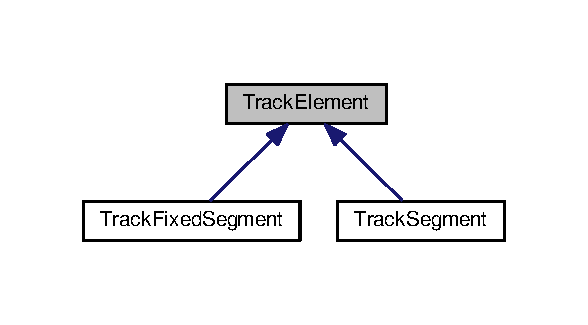
\includegraphics[width=282pt]{classKite_1_1TrackElement__inherit__graph}
\end{center}
\end{figure}
\subsubsection*{Public Member Functions}
\begin{DoxyCompactItemize}
\item 
virtual bool \hyperlink{classKite_1_1TrackElement_af5e7d3badddf2ec07159f1d83426d4c1}{is\-Fixed} () const 
\item 
virtual bool \hyperlink{classKite_1_1TrackElement_a9d3db1f8a5aca58f8f54d291faebf873}{is\-Horizontal} () const =0
\item 
virtual bool \hyperlink{classKite_1_1TrackElement_a6fa2bf0568a2b295dd7cd1f7207247d5}{is\-Vertical} () const =0
\item 
virtual bool \hyperlink{classKite_1_1TrackElement_a69fb7e260ed2bc6fa82bfe12c2aeec5a}{is\-Local} () const 
\item 
virtual bool \hyperlink{classKite_1_1TrackElement_a017b1ead8e5988dd0e491cae93ac510c}{is\-Global} () const 
\item 
virtual bool \hyperlink{classKite_1_1TrackElement_ab5035e6d84cf3ec7b519a5acb109efaa}{is\-Bipoint} () const 
\item 
virtual bool \hyperlink{classKite_1_1TrackElement_a8d6f4521b27f32080d7477cf8ee8a274}{is\-Terminal} () const 
\item 
virtual bool \hyperlink{classKite_1_1TrackElement_a4721fcbe9c93ed5392afd9a756b989a8}{is\-Strap} () const 
\item 
virtual bool \hyperlink{classKite_1_1TrackElement_ab1f9e0bca70dea59558459a003a62d88}{is\-Slackened} () const 
\item 
virtual bool \hyperlink{classKite_1_1TrackElement_a172b2394f9c2cbaaf5bc4b19e0e76e65}{is\-Dogleg} () const 
\item 
bool \hyperlink{classKite_1_1TrackElement_a6a7e35dd5a9ca99ca879e424ce42b902}{is\-Created} () const 
\item 
bool \hyperlink{classKite_1_1TrackElement_a54f713d06c43bebf4e0dfef06e347531}{is\-Invalidated} () const 
\item 
bool \hyperlink{classKite_1_1TrackElement_a1dbaf905a283e4e45ac71c4771e9e644}{is\-Blockage} () const 
\item 
bool \hyperlink{classKite_1_1TrackElement_ae0c9fa9daf2467984aea571a0f3940c6}{is\-Locked} () const 
\item 
bool \hyperlink{classKite_1_1TrackElement_ae7adbfe4ada0ac46f8cd9cc8f296327d}{is\-Routed} () const 
\item 
bool \hyperlink{classKite_1_1TrackElement_af5f88959753a39f16726a858ee6fb0fd}{has\-Source\-Dogleg} () const 
\item 
bool \hyperlink{classKite_1_1TrackElement_a71fcabadfc78d0e1aefa934659cb1204}{has\-Target\-Dogleg} () const 
\item 
bool \hyperlink{classKite_1_1TrackElement_a5aa65e9913c7368130b187464404ded6}{can\-Ripple} () const 
\item 
virtual bool \hyperlink{classKite_1_1TrackElement_aa0bb6f1592688e942ff67e0ac318a4fd}{can\-Dogleg} ()
\item 
virtual bool \hyperlink{classKite_1_1TrackElement_accb4c6a7ee2678a0cff4dbc4a7860fe1}{can\-Dogleg} ({\bf Interval})
\item 
virtual bool \hyperlink{classKite_1_1TrackElement_a4f040cf33009e4886d401115c3bea838}{can\-Dogleg} ({\bf Katabatic\-::\-G\-Cell} $\ast$, unsigned int flags=0)
\item 
virtual unsigned long \hyperlink{classKite_1_1TrackElement_ae68c47fdf838be02cbf6660cd25a0806}{get\-Id} () const 
\item 
virtual unsigned int \hyperlink{classKite_1_1TrackElement_ae35b78590ed6aa546b626ef95f28c533}{get\-Direction} () const =0
\item 
virtual {\bf Net} $\ast$ \hyperlink{classKite_1_1TrackElement_a2b383a5b6f5028911a35e446a682dabd}{get\-Net} () const =0
\item 
virtual const {\bf Layer} $\ast$ \hyperlink{classKite_1_1TrackElement_ad96c66549598873bf68c2e18ec7164c1}{get\-Layer} () const =0
\item 
\hyperlink{classKite_1_1Track}{Track} $\ast$ \hyperlink{classKite_1_1TrackElement_abfd8de286baf41eea066220773c7046d}{get\-Track} () const 
\item 
size\-\_\-t \hyperlink{classKite_1_1TrackElement_a659e8df65f89db5547aa8a8fe3d92f69}{get\-Index} () const 
\item 
virtual unsigned long \hyperlink{classKite_1_1TrackElement_a9f20f94d2d8aaa38c2b9ead5275ead27}{get\-Freedom\-Degree} () const 
\item 
virtual float \hyperlink{classKite_1_1TrackElement_a71b29fb20a3ba09616a6be4b122a797e}{get\-Max\-Under\-Density} (unsigned int flags=0) const 
\item 
{\bf Box} \hyperlink{classKite_1_1TrackElement_a3b9694bf093e3ea16e4a8c8126a8d4db}{get\-Bounding\-Box} () const 
\item 
virtual \hyperlink{classKite_1_1TrackElement}{Track\-Element} $\ast$ \hyperlink{classKite_1_1TrackElement_a5af0ac91c558873fea9703e7ab6f48df}{get\-Next} () const 
\item 
virtual \hyperlink{classKite_1_1TrackElement}{Track\-Element} $\ast$ \hyperlink{classKite_1_1TrackElement_acbb9c965449bf4502d71149563cec0a2}{get\-Previous} () const 
\item 
virtual {\bf Db\-U\-::\-Unit} \hyperlink{classKite_1_1TrackElement_ac492fb5399691d81c31547db6b56fd03}{get\-Axis} () const =0
\item 
{\bf Db\-U\-::\-Unit} \hyperlink{classKite_1_1TrackElement_a3932d5ce9094ead510e4e33bd4e78e1a}{get\-Source\-U} () const 
\item 
{\bf Db\-U\-::\-Unit} \hyperlink{classKite_1_1TrackElement_a8e5f2a51f56c6bdb74024ac77c08a22a}{get\-Target\-U} () const 
\item 
{\bf Db\-U\-::\-Unit} \hyperlink{classKite_1_1TrackElement_a5370f2cf21823e1fa58d0627ee53c483}{get\-Length} () const 
\item 
{\bf Interval} \hyperlink{classKite_1_1TrackElement_ad78cfb34e7d8e92ba854fbc2dbf9d842}{get\-Canonical\-Interval} () const 
\item 
virtual {\bf Interval} \hyperlink{classKite_1_1TrackElement_a38d30a241d00a14943a06401d0d12923}{get\-Free\-Interval} () const 
\item 
virtual {\bf Interval} \hyperlink{classKite_1_1TrackElement_a972921aeb7f907194710ea35ac7600be}{get\-Source\-Constraints} () const 
\item 
virtual {\bf Interval} \hyperlink{classKite_1_1TrackElement_a00d398bdc1837c6c1e4847895c557829}{get\-Target\-Constraints} () const 
\item 
virtual \hyperlink{classKite_1_1DataNegociate}{Data\-Negociate} $\ast$ \hyperlink{classKite_1_1TrackElement_a76a45d5701f875711a03692e9bf6d5ce}{get\-Data\-Negociate} (unsigned int flags=\hyperlink{namespaceKite_acca8fffa3182dea5f94208f454f14b47a68e917ff37d4b5cef906303181836404}{Kt\-Data\-Self}) const 
\item 
virtual \hyperlink{classKite_1_1TrackElement}{Track\-Element} $\ast$ \hyperlink{classKite_1_1TrackElement_af2d46d64cbd02bdbba53d5483d95e26d}{get\-Canonical} ({\bf Interval} \&)
\item 
virtual size\-\_\-t \hyperlink{classKite_1_1TrackElement_a79b25d8199fe90446e99cf08d2d85674}{get\-G\-Cells} (Katabatic\-::\-G\-Cell\-Vector \&) const 
\item 
virtual \hyperlink{classKite_1_1TrackElement}{Track\-Element} $\ast$ \hyperlink{classKite_1_1TrackElement_ad1a03a36d5908ce44c3d0391ff9c7103}{get\-Parent} () const 
\item 
virtual unsigned int \hyperlink{classKite_1_1TrackElement_ace669b962e7df815b92fe70e1f4ad755}{get\-Dogleg\-Level} () const 
\item 
virtual \hyperlink{classKite_1_1TrackElement}{Track\-Element} $\ast$ \hyperlink{classKite_1_1TrackElement_a7e79fbfe77f173d46b1959c41087930a}{get\-Source\-Dogleg} ()
\item 
virtual \hyperlink{classKite_1_1TrackElement}{Track\-Element} $\ast$ \hyperlink{classKite_1_1TrackElement_aeb4e39bd925d093e6c45599433bb421c}{get\-Target\-Dogleg} ()
\item 
virtual Track\-Elements \hyperlink{classKite_1_1TrackElement_aa0ba92ebf19f596537dc051c090d5736}{get\-Perpandiculars} ()
\item 
void \hyperlink{classKite_1_1TrackElement_aeb14f94914af58657a0dc2f50ec98df5}{set\-Flags} (unsigned int)
\item 
void \hyperlink{classKite_1_1TrackElement_a1a6fac115cb81db48e3ac9ffa0721bb5}{unset\-Flags} (unsigned int)
\item 
virtual void \hyperlink{classKite_1_1TrackElement_abd3d8093f871d3d1a7f24b053648026c}{set\-Track} (\hyperlink{classKite_1_1Track}{Track} $\ast$)
\item 
void \hyperlink{classKite_1_1TrackElement_abee236b4d62f51320212f31e010fc1b5}{set\-Index} (size\-\_\-t)
\item 
virtual void \hyperlink{classKite_1_1TrackElement_af5332d647c0482aa90ad7cc9b2a50f3a}{update\-Freedom\-Degree} ()
\item 
virtual void \hyperlink{classKite_1_1TrackElement_a2b90319cb042b283aa5d1fdb1992f11f}{set\-Dogleg\-Level} (unsigned int)
\item 
virtual void \hyperlink{classKite_1_1TrackElement_acc245ce084989d1c34816d0e61b9d510}{swap\-Track} (\hyperlink{classKite_1_1TrackElement}{Track\-Element} $\ast$)
\item 
virtual void \hyperlink{classKite_1_1TrackElement_a0ffe603ec7d46f21f5e56ccbe84c03fb}{reschedule} (unsigned int level)
\item 
virtual void \hyperlink{classKite_1_1TrackElement_ac295bade8aee589f6718dfa79edc2a34}{detach} ()
\item 
virtual void \hyperlink{classKite_1_1TrackElement_a893f1101c650c08c98612515c2b1a89c}{invalidate} ()
\item 
virtual void \hyperlink{classKite_1_1TrackElement_a5bd93abe1416952ace15a98dbeeed124}{revalidate} ()
\item 
virtual void \hyperlink{classKite_1_1TrackElement_a250348f9030b92b19580749bf99030b5}{inc\-Overlap\-Cost} ({\bf Net} $\ast$, Track\-Cost \&) const 
\item 
virtual void \hyperlink{classKite_1_1TrackElement_a45e685b1e3ee630d24bf43746553af4c}{set\-Axis} ({\bf Db\-U\-::\-Unit}, unsigned int flags={\bf Katabatic\-::\-Seg\-Axis\-Set})
\item 
virtual \hyperlink{classKite_1_1TrackElement}{Track\-Element} $\ast$ \hyperlink{classKite_1_1TrackElement_a7a9637875364e84e6862de0102341715}{make\-Dogleg} ()
\item 
bool \hyperlink{classKite_1_1TrackElement_a3e1b4982a2427f74e55592520ab6272d}{make\-Dogleg} ({\bf Katabatic\-::\-G\-Cell} $\ast$)
\item 
virtual \hyperlink{classKite_1_1TrackElement}{Track\-Element} $\ast$ \hyperlink{classKite_1_1TrackElement_a524f1569b2f2c1a84df2fe47e84e28ed}{make\-Dogleg} ({\bf Interval}, unsigned int \&flags)
\item 
virtual bool \hyperlink{classKite_1_1TrackElement_aa1ef325b98fab61d2c7c5bdc1fcd92fc}{\-\_\-check} () const 
\end{DoxyCompactItemize}
\subsubsection*{Static Public Member Functions}
\begin{DoxyCompactItemize}
\item 
static \hyperlink{namespaceKite_aa5bc3df660243357cdf8639f57d4a41b}{Segment\-Overlap\-Cost\-C\-B} $\ast$ \hyperlink{classKite_1_1TrackElement_a4648fa47d0870cf743436ff6a6239fd9}{set\-Overlap\-Cost\-C\-B} (\hyperlink{namespaceKite_aa5bc3df660243357cdf8639f57d4a41b}{Segment\-Overlap\-Cost\-C\-B} $\ast$)
\end{DoxyCompactItemize}


\subsubsection{Detailed Description}
Abstract Class for all Elements inserted inside a \hyperlink{classKite_1_1Track}{Track}. 

\hypertarget{classKite_1_1TrackElement_secTrackElementAbstract}{}\subsubsection{Track\-Element Abstract}\label{classKite_1_1TrackElement_secTrackElementAbstract}
The \hyperlink{classKite_1_1TrackElement}{Track\-Element} class is abstract and is used as base class for any element that can be inserted in a \hyperlink{classKite_1_1Track}{Track}. It represent the footprint of that element inside the \hyperlink{classKite_1_1Track}{Track} (an interval). Additionnaly it keep a pointer to the \hyperlink{classKite_1_1Track}{Track} and it's index inside it (\hyperlink{classKite_1_1Track}{Track} is implemented with a {\ttfamily vector$<$$>$}).

To avoid some explicit dynamic cast later, it provides a default implementation for almost all the methods that will be present in all the derived classes. All default methods return {\ttfamily false}, {\ttfamily N\-U\-L\-L} or {\ttfamily 0} ({\itshape zero}) or whatever is appropriated to tell it is not meaningful.

{\bfseries Design Note}

\hyperlink{classKite_1_1TrackElement}{Track\-Element} has been designed to serve as a base class for \hyperlink{classKite_1_1TrackSegment}{Track\-Segment} and \hyperlink{classKite_1_1TrackMarker}{Track\-Marker}. But, in the end, those two classes have been put in separated vectors inside the \hyperlink{classKite_1_1Track}{Track}, thus rendering this design choice less pertinent. We keep it for now because we may introduce other object than \hyperlink{classKite_1_1TrackSegment}{Track\-Segment} inside a \hyperlink{classKite_1_1Track}{Track}. If the need do not arise, we may merge back \hyperlink{classKite_1_1TrackElement}{Track\-Element} and \hyperlink{classKite_1_1TrackSegment}{Track\-Segment}. 

\subsubsection{Member Function Documentation}
\hypertarget{classKite_1_1TrackElement_a4648fa47d0870cf743436ff6a6239fd9}{\index{Kite\-::\-Track\-Element@{Kite\-::\-Track\-Element}!set\-Overlap\-Cost\-C\-B@{set\-Overlap\-Cost\-C\-B}}
\index{set\-Overlap\-Cost\-C\-B@{set\-Overlap\-Cost\-C\-B}!Kite::TrackElement@{Kite\-::\-Track\-Element}}
\paragraph[{set\-Overlap\-Cost\-C\-B}]{\setlength{\rightskip}{0pt plus 5cm}{\bf Segment\-Overlap\-Cost\-C\-B} $\ast$ set\-Overlap\-Cost\-C\-B (
\begin{DoxyParamCaption}
\item[{{\bf Segment\-Overlap\-Cost\-C\-B} $\ast$}]{cb}
\end{DoxyParamCaption}
)\hspace{0.3cm}{\ttfamily [static]}}}\label{classKite_1_1TrackElement_a4648fa47d0870cf743436ff6a6239fd9}

\begin{DoxyParams}{Parameters}
{\em cb} & the new overlap cost callback. \\
\hline
\end{DoxyParams}
\begin{DoxyReturn}{Returns}
the previous overlap cost callback.
\end{DoxyReturn}
sets the overlap callback. 

Referenced by Negociate\-Window\-::run().

\hypertarget{classKite_1_1TrackElement_af5e7d3badddf2ec07159f1d83426d4c1}{\index{Kite\-::\-Track\-Element@{Kite\-::\-Track\-Element}!is\-Fixed@{is\-Fixed}}
\index{is\-Fixed@{is\-Fixed}!Kite::TrackElement@{Kite\-::\-Track\-Element}}
\paragraph[{is\-Fixed}]{\setlength{\rightskip}{0pt plus 5cm}bool is\-Fixed (
\begin{DoxyParamCaption}
{}
\end{DoxyParamCaption}
) const\hspace{0.3cm}{\ttfamily [virtual]}}}\label{classKite_1_1TrackElement_af5e7d3badddf2ec07159f1d83426d4c1}
{\bfseries See also\-:}~ {\bf Katabatic\-::\-Auto\-Segment\-::is\-Fixed()}. 

Reimplemented in \hyperlink{classKite_1_1TrackSegment_af5e7d3badddf2ec07159f1d83426d4c1}{Track\-Segment}, and \hyperlink{classKite_1_1TrackFixedSegment_af5e7d3badddf2ec07159f1d83426d4c1}{Track\-Fixed\-Segment}.



Referenced by Segment\-Fsm\-::add\-Action(), Segment\-Fsm\-::conflict\-Solve\-By\-Placeds(), Negociate\-Window\-::create\-Track\-Segment(), Segment\-Fsm\-::desaturate(), Segment\-Action\-::do\-Action(), Manipulator\-::force\-Over\-Locals(), Manipulator\-::force\-To\-Track(), Manipulator\-::insert\-In\-Track(), Manipulator\-::is\-Caged(), Manipulator\-::make\-Dogleg(), Manipulator\-::minimize(), Manipulator\-::move\-Up(), Manipulator\-::pivot\-Down(), Manipulator\-::pivot\-Up(), Manipulator\-::relax(), Manipulator\-::repack\-Perpandiculars(), Manipulator\-::ripup(), Manipulator\-::shrink\-To\-Track(), and Manipulator\-::slacken().

\hypertarget{classKite_1_1TrackElement_a9d3db1f8a5aca58f8f54d291faebf873}{\index{Kite\-::\-Track\-Element@{Kite\-::\-Track\-Element}!is\-Horizontal@{is\-Horizontal}}
\index{is\-Horizontal@{is\-Horizontal}!Kite::TrackElement@{Kite\-::\-Track\-Element}}
\paragraph[{is\-Horizontal}]{\setlength{\rightskip}{0pt plus 5cm}bool is\-Horizontal (
\begin{DoxyParamCaption}
{}
\end{DoxyParamCaption}
) const\hspace{0.3cm}{\ttfamily [pure virtual]}}}\label{classKite_1_1TrackElement_a9d3db1f8a5aca58f8f54d291faebf873}
{\bfseries See also\-:}~ {\bf Katabatic\-::\-Auto\-Segment\-::is\-Horizontal()}. 

Implemented in \hyperlink{classKite_1_1TrackSegment_ac46ac3b48d712750c7888b48964ac189}{Track\-Segment}, and \hyperlink{classKite_1_1TrackFixedSegment_ac46ac3b48d712750c7888b48964ac189}{Track\-Fixed\-Segment}.



Referenced by Segment\-Fsm\-::conflict\-Solve\-By\-History(), and Manipulator\-::make\-Dogleg().

\hypertarget{classKite_1_1TrackElement_a6fa2bf0568a2b295dd7cd1f7207247d5}{\index{Kite\-::\-Track\-Element@{Kite\-::\-Track\-Element}!is\-Vertical@{is\-Vertical}}
\index{is\-Vertical@{is\-Vertical}!Kite::TrackElement@{Kite\-::\-Track\-Element}}
\paragraph[{is\-Vertical}]{\setlength{\rightskip}{0pt plus 5cm}bool is\-Vertical (
\begin{DoxyParamCaption}
{}
\end{DoxyParamCaption}
) const\hspace{0.3cm}{\ttfamily [pure virtual]}}}\label{classKite_1_1TrackElement_a6fa2bf0568a2b295dd7cd1f7207247d5}
{\bfseries See also\-:}~ {\bf Katabatic\-::\-Auto\-Segment\-::is\-Vertical()}. 

Implemented in \hyperlink{classKite_1_1TrackSegment_a2bb30e82aad1f321af4a065338775f36}{Track\-Segment}, and \hyperlink{classKite_1_1TrackFixedSegment_a2bb30e82aad1f321af4a065338775f36}{Track\-Fixed\-Segment}.

\hypertarget{classKite_1_1TrackElement_a69fb7e260ed2bc6fa82bfe12c2aeec5a}{\index{Kite\-::\-Track\-Element@{Kite\-::\-Track\-Element}!is\-Local@{is\-Local}}
\index{is\-Local@{is\-Local}!Kite::TrackElement@{Kite\-::\-Track\-Element}}
\paragraph[{is\-Local}]{\setlength{\rightskip}{0pt plus 5cm}bool is\-Local (
\begin{DoxyParamCaption}
{}
\end{DoxyParamCaption}
) const\hspace{0.3cm}{\ttfamily [virtual]}}}\label{classKite_1_1TrackElement_a69fb7e260ed2bc6fa82bfe12c2aeec5a}
{\bfseries See also\-:}~ Katabatic\-::is\-Local(). 

Reimplemented in \hyperlink{classKite_1_1TrackSegment_a69fb7e260ed2bc6fa82bfe12c2aeec5a}{Track\-Segment}.



Referenced by Segment\-Fsm\-::conflict\-Solve\-By\-Placeds(), Segment\-Fsm\-::do\-Actions(), Manipulator\-::insert\-In\-Track(), Manipulator\-::make\-Dogleg(), Manipulator\-::move\-Up(), Manipulator\-::pivot\-Up(), Manipulator\-::relax(), Manipulator\-::ripple(), Manipulator\-::ripup\-Perpandiculars(), Segment\-Fsm\-::\-Segment\-Fsm(), Manipulator\-::shrink\-To\-Track(), Segment\-Fsm\-::slacken\-Topology(), and Segment\-Fsm\-::solve\-Full\-Blockages().

\hypertarget{classKite_1_1TrackElement_a017b1ead8e5988dd0e491cae93ac510c}{\index{Kite\-::\-Track\-Element@{Kite\-::\-Track\-Element}!is\-Global@{is\-Global}}
\index{is\-Global@{is\-Global}!Kite::TrackElement@{Kite\-::\-Track\-Element}}
\paragraph[{is\-Global}]{\setlength{\rightskip}{0pt plus 5cm}bool is\-Global (
\begin{DoxyParamCaption}
{}
\end{DoxyParamCaption}
) const\hspace{0.3cm}{\ttfamily [virtual]}}}\label{classKite_1_1TrackElement_a017b1ead8e5988dd0e491cae93ac510c}
{\bfseries See also\-:}~ {\bf Katabatic\-::\-Auto\-Segment\-::is\-Global()}. 

Reimplemented in \hyperlink{classKite_1_1TrackSegment_a017b1ead8e5988dd0e491cae93ac510c}{Track\-Segment}.



Referenced by Segment\-Fsm\-::conflict\-Solve\-By\-Placeds(), Manipulator\-::insert\-In\-Track(), Manipulator\-::relax(), Manipulator\-::repack\-Perpandiculars(), and Segment\-Fsm\-::\-Segment\-Fsm().

\hypertarget{classKite_1_1TrackElement_ab5035e6d84cf3ec7b519a5acb109efaa}{\index{Kite\-::\-Track\-Element@{Kite\-::\-Track\-Element}!is\-Bipoint@{is\-Bipoint}}
\index{is\-Bipoint@{is\-Bipoint}!Kite::TrackElement@{Kite\-::\-Track\-Element}}
\paragraph[{is\-Bipoint}]{\setlength{\rightskip}{0pt plus 5cm}bool is\-Bipoint (
\begin{DoxyParamCaption}
{}
\end{DoxyParamCaption}
) const\hspace{0.3cm}{\ttfamily [virtual]}}}\label{classKite_1_1TrackElement_ab5035e6d84cf3ec7b519a5acb109efaa}
{\bfseries See also\-:}~ {\bf Katabatic\-::\-Auto\-Segment\-::is\-Bipoint()}. 

Reimplemented in \hyperlink{classKite_1_1TrackSegment_ab5035e6d84cf3ec7b519a5acb109efaa}{Track\-Segment}.



Referenced by Segment\-Fsm\-::desaturate().

\hypertarget{classKite_1_1TrackElement_a8d6f4521b27f32080d7477cf8ee8a274}{\index{Kite\-::\-Track\-Element@{Kite\-::\-Track\-Element}!is\-Terminal@{is\-Terminal}}
\index{is\-Terminal@{is\-Terminal}!Kite::TrackElement@{Kite\-::\-Track\-Element}}
\paragraph[{is\-Terminal}]{\setlength{\rightskip}{0pt plus 5cm}bool is\-Terminal (
\begin{DoxyParamCaption}
{}
\end{DoxyParamCaption}
) const\hspace{0.3cm}{\ttfamily [virtual]}}}\label{classKite_1_1TrackElement_a8d6f4521b27f32080d7477cf8ee8a274}
{\bfseries See also\-:}~ Katabatic\-::\-Auto\-Segment\-::is\-Terminal(). 

Reimplemented in \hyperlink{classKite_1_1TrackSegment_a8d6f4521b27f32080d7477cf8ee8a274}{Track\-Segment}.



Referenced by Manipulator\-::make\-Dogleg(), and Manipulator\-::relax().

\hypertarget{classKite_1_1TrackElement_a4721fcbe9c93ed5392afd9a756b989a8}{\index{Kite\-::\-Track\-Element@{Kite\-::\-Track\-Element}!is\-Strap@{is\-Strap}}
\index{is\-Strap@{is\-Strap}!Kite::TrackElement@{Kite\-::\-Track\-Element}}
\paragraph[{is\-Strap}]{\setlength{\rightskip}{0pt plus 5cm}bool is\-Strap (
\begin{DoxyParamCaption}
{}
\end{DoxyParamCaption}
) const\hspace{0.3cm}{\ttfamily [virtual]}}}\label{classKite_1_1TrackElement_a4721fcbe9c93ed5392afd9a756b989a8}
{\bfseries See also\-:}~ {\bf Katabatic\-::\-Auto\-Segment\-::is\-Strap()}. 

Reimplemented in \hyperlink{classKite_1_1TrackSegment_a4721fcbe9c93ed5392afd9a756b989a8}{Track\-Segment}.



Referenced by Manipulator\-::insert\-In\-Track(), Manipulator\-::pivot\-Down(), Manipulator\-::pivot\-Up(), Segment\-Fsm\-::\-Segment\-Fsm(), and Segment\-Fsm\-::slacken\-Topology().

\hypertarget{classKite_1_1TrackElement_ab1f9e0bca70dea59558459a003a62d88}{\index{Kite\-::\-Track\-Element@{Kite\-::\-Track\-Element}!is\-Slackened@{is\-Slackened}}
\index{is\-Slackened@{is\-Slackened}!Kite::TrackElement@{Kite\-::\-Track\-Element}}
\paragraph[{is\-Slackened}]{\setlength{\rightskip}{0pt plus 5cm}bool is\-Slackened (
\begin{DoxyParamCaption}
{}
\end{DoxyParamCaption}
) const\hspace{0.3cm}{\ttfamily [virtual]}}}\label{classKite_1_1TrackElement_ab1f9e0bca70dea59558459a003a62d88}
{\bfseries See also\-:}~ {\bf Katabatic\-::\-Auto\-Segment\-::is\-Slackened()}. 

Reimplemented in \hyperlink{classKite_1_1TrackSegment_ab1f9e0bca70dea59558459a003a62d88}{Track\-Segment}.

\hypertarget{classKite_1_1TrackElement_a172b2394f9c2cbaaf5bc4b19e0e76e65}{\index{Kite\-::\-Track\-Element@{Kite\-::\-Track\-Element}!is\-Dogleg@{is\-Dogleg}}
\index{is\-Dogleg@{is\-Dogleg}!Kite::TrackElement@{Kite\-::\-Track\-Element}}
\paragraph[{is\-Dogleg}]{\setlength{\rightskip}{0pt plus 5cm}bool is\-Dogleg (
\begin{DoxyParamCaption}
{}
\end{DoxyParamCaption}
) const\hspace{0.3cm}{\ttfamily [virtual]}}}\label{classKite_1_1TrackElement_a172b2394f9c2cbaaf5bc4b19e0e76e65}
{\bfseries See also\-:}~ Katabatic\-::is\-Dogleg(). 

Reimplemented in \hyperlink{classKite_1_1TrackSegment_a172b2394f9c2cbaaf5bc4b19e0e76e65}{Track\-Segment}.

\hypertarget{classKite_1_1TrackElement_a6a7e35dd5a9ca99ca879e424ce42b902}{\index{Kite\-::\-Track\-Element@{Kite\-::\-Track\-Element}!is\-Created@{is\-Created}}
\index{is\-Created@{is\-Created}!Kite::TrackElement@{Kite\-::\-Track\-Element}}
\paragraph[{is\-Created}]{\setlength{\rightskip}{0pt plus 5cm}bool is\-Created (
\begin{DoxyParamCaption}
{}
\end{DoxyParamCaption}
) const\hspace{0.3cm}{\ttfamily [inline]}}}\label{classKite_1_1TrackElement_a6a7e35dd5a9ca99ca879e424ce42b902}
{\bfseries See also\-:}~ {\bf Katabatic\-::\-Auto\-Segment\-::is\-Created()}. \hypertarget{classKite_1_1TrackElement_a54f713d06c43bebf4e0dfef06e347531}{\index{Kite\-::\-Track\-Element@{Kite\-::\-Track\-Element}!is\-Invalidated@{is\-Invalidated}}
\index{is\-Invalidated@{is\-Invalidated}!Kite::TrackElement@{Kite\-::\-Track\-Element}}
\paragraph[{is\-Invalidated}]{\setlength{\rightskip}{0pt plus 5cm}bool is\-Invalidated (
\begin{DoxyParamCaption}
{}
\end{DoxyParamCaption}
) const\hspace{0.3cm}{\ttfamily [inline]}}}\label{classKite_1_1TrackElement_a54f713d06c43bebf4e0dfef06e347531}
{\bfseries Returns\-:} {\bfseries true} if the segment is invalidated (may be different from the supporting Auto\-Segment status). 

Referenced by Segment\-Observer\-::notify().

\hypertarget{classKite_1_1TrackElement_a1dbaf905a283e4e45ac71c4771e9e644}{\index{Kite\-::\-Track\-Element@{Kite\-::\-Track\-Element}!is\-Blockage@{is\-Blockage}}
\index{is\-Blockage@{is\-Blockage}!Kite::TrackElement@{Kite\-::\-Track\-Element}}
\paragraph[{is\-Blockage}]{\setlength{\rightskip}{0pt plus 5cm}bool is\-Blockage (
\begin{DoxyParamCaption}
{}
\end{DoxyParamCaption}
) const\hspace{0.3cm}{\ttfamily [inline]}}}\label{classKite_1_1TrackElement_a1dbaf905a283e4e45ac71c4771e9e644}
{\bfseries true} if the element is a blockage (obstacle). 

Referenced by Segment\-Fsm\-::conflict\-Solve\-By\-Placeds(), Negociate\-Window\-::create\-Track\-Segment(), Manipulator\-::insert\-In\-Track(), and Manipulator\-::is\-Caged().

\hypertarget{classKite_1_1TrackElement_ae0c9fa9daf2467984aea571a0f3940c6}{\index{Kite\-::\-Track\-Element@{Kite\-::\-Track\-Element}!is\-Locked@{is\-Locked}}
\index{is\-Locked@{is\-Locked}!Kite::TrackElement@{Kite\-::\-Track\-Element}}
\paragraph[{is\-Locked}]{\setlength{\rightskip}{0pt plus 5cm}bool is\-Locked (
\begin{DoxyParamCaption}
{}
\end{DoxyParamCaption}
) const\hspace{0.3cm}{\ttfamily [inline]}}}\label{classKite_1_1TrackElement_ae0c9fa9daf2467984aea571a0f3940c6}
{\bfseries true} if the element is part of a net, but must not be moved by the router, whatever the reason. \hypertarget{classKite_1_1TrackElement_ae7adbfe4ada0ac46f8cd9cc8f296327d}{\index{Kite\-::\-Track\-Element@{Kite\-::\-Track\-Element}!is\-Routed@{is\-Routed}}
\index{is\-Routed@{is\-Routed}!Kite::TrackElement@{Kite\-::\-Track\-Element}}
\paragraph[{is\-Routed}]{\setlength{\rightskip}{0pt plus 5cm}bool is\-Routed (
\begin{DoxyParamCaption}
{}
\end{DoxyParamCaption}
) const\hspace{0.3cm}{\ttfamily [inline]}}}\label{classKite_1_1TrackElement_ae7adbfe4ada0ac46f8cd9cc8f296327d}
{\bfseries true} if the router has placed it. 

Referenced by Track\-Segment\-::can\-Dogleg().

\hypertarget{classKite_1_1TrackElement_af5f88959753a39f16726a858ee6fb0fd}{\index{Kite\-::\-Track\-Element@{Kite\-::\-Track\-Element}!has\-Source\-Dogleg@{has\-Source\-Dogleg}}
\index{has\-Source\-Dogleg@{has\-Source\-Dogleg}!Kite::TrackElement@{Kite\-::\-Track\-Element}}
\paragraph[{has\-Source\-Dogleg}]{\setlength{\rightskip}{0pt plus 5cm}bool has\-Source\-Dogleg (
\begin{DoxyParamCaption}
{}
\end{DoxyParamCaption}
) const\hspace{0.3cm}{\ttfamily [inline]}}}\label{classKite_1_1TrackElement_af5f88959753a39f16726a858ee6fb0fd}
This method purpose has not been reviewed yet. 

Referenced by Track\-Segment\-::can\-Dogleg(), Track\-Segment\-::get\-Source\-Dogleg(), and Track\-Segment\-::get\-Target\-Dogleg().

\hypertarget{classKite_1_1TrackElement_a71fcabadfc78d0e1aefa934659cb1204}{\index{Kite\-::\-Track\-Element@{Kite\-::\-Track\-Element}!has\-Target\-Dogleg@{has\-Target\-Dogleg}}
\index{has\-Target\-Dogleg@{has\-Target\-Dogleg}!Kite::TrackElement@{Kite\-::\-Track\-Element}}
\paragraph[{has\-Target\-Dogleg}]{\setlength{\rightskip}{0pt plus 5cm}bool has\-Target\-Dogleg (
\begin{DoxyParamCaption}
{}
\end{DoxyParamCaption}
) const\hspace{0.3cm}{\ttfamily [inline]}}}\label{classKite_1_1TrackElement_a71fcabadfc78d0e1aefa934659cb1204}
This method purpose has not been reviewed yet. 

Referenced by Track\-Segment\-::can\-Dogleg().

\hypertarget{classKite_1_1TrackElement_a5aa65e9913c7368130b187464404ded6}{\index{Kite\-::\-Track\-Element@{Kite\-::\-Track\-Element}!can\-Ripple@{can\-Ripple}}
\index{can\-Ripple@{can\-Ripple}!Kite::TrackElement@{Kite\-::\-Track\-Element}}
\paragraph[{can\-Ripple}]{\setlength{\rightskip}{0pt plus 5cm}bool can\-Ripple (
\begin{DoxyParamCaption}
{}
\end{DoxyParamCaption}
) const\hspace{0.3cm}{\ttfamily [inline]}}}\label{classKite_1_1TrackElement_a5aa65e9913c7368130b187464404ded6}
This method purpose has not been reviewed yet. 

Referenced by Manipulator\-::ripple().

\hypertarget{classKite_1_1TrackElement_aa0bb6f1592688e942ff67e0ac318a4fd}{\index{Kite\-::\-Track\-Element@{Kite\-::\-Track\-Element}!can\-Dogleg@{can\-Dogleg}}
\index{can\-Dogleg@{can\-Dogleg}!Kite::TrackElement@{Kite\-::\-Track\-Element}}
\paragraph[{can\-Dogleg}]{\setlength{\rightskip}{0pt plus 5cm}bool can\-Dogleg (
\begin{DoxyParamCaption}
{}
\end{DoxyParamCaption}
)\hspace{0.3cm}{\ttfamily [virtual]}}}\label{classKite_1_1TrackElement_aa0bb6f1592688e942ff67e0ac318a4fd}
{\bfseries See also\-:}~ {\bf Auto\-Segment\-::can\-Dogleg()}. At \hyperlink{namespaceKite}{Kite} level, this variant of the method will apply only on local segments and the segment must not already have a source or target dogleg. 

Reimplemented in \hyperlink{classKite_1_1TrackSegment_aa0bb6f1592688e942ff67e0ac318a4fd}{Track\-Segment}.



Referenced by Segment\-Fsm\-::conflict\-Solve\-By\-History(), Manipulator\-::make\-Dogleg(), and Manipulator\-::relax().

\hypertarget{classKite_1_1TrackElement_accb4c6a7ee2678a0cff4dbc4a7860fe1}{\index{Kite\-::\-Track\-Element@{Kite\-::\-Track\-Element}!can\-Dogleg@{can\-Dogleg}}
\index{can\-Dogleg@{can\-Dogleg}!Kite::TrackElement@{Kite\-::\-Track\-Element}}
\paragraph[{can\-Dogleg}]{\setlength{\rightskip}{0pt plus 5cm}bool can\-Dogleg (
\begin{DoxyParamCaption}
\item[{{\bf Interval}}]{}
\end{DoxyParamCaption}
)\hspace{0.3cm}{\ttfamily [virtual]}}}\label{classKite_1_1TrackElement_accb4c6a7ee2678a0cff4dbc4a7860fe1}
{\bfseries See also\-:}~ {\bf Auto\-Segment\-::can\-Dogleg()}. At \hyperlink{namespaceKite}{Kite} level, this variant of the method will apply only on local segments and the segment must not already have a source or target dogleg. 

Reimplemented in \hyperlink{classKite_1_1TrackSegment_accb4c6a7ee2678a0cff4dbc4a7860fe1}{Track\-Segment}.

\hypertarget{classKite_1_1TrackElement_a4f040cf33009e4886d401115c3bea838}{\index{Kite\-::\-Track\-Element@{Kite\-::\-Track\-Element}!can\-Dogleg@{can\-Dogleg}}
\index{can\-Dogleg@{can\-Dogleg}!Kite::TrackElement@{Kite\-::\-Track\-Element}}
\paragraph[{can\-Dogleg}]{\setlength{\rightskip}{0pt plus 5cm}bool can\-Dogleg (
\begin{DoxyParamCaption}
\item[{{\bf Katabatic\-::\-G\-Cell} $\ast$}]{dogleg\-G\-Cell, }
\item[{unsigned int}]{flags = {\ttfamily 0}}
\end{DoxyParamCaption}
)\hspace{0.3cm}{\ttfamily [virtual]}}}\label{classKite_1_1TrackElement_a4f040cf33009e4886d401115c3bea838}
{\bfseries See also\-:}~ {\bf Auto\-Segment\-::can\-Dogleg()}. At kite level, this variant of the method is mainly targeted to global segment. For local segment it behave like \hyperlink{classKite_1_1TrackElement_accb4c6a7ee2678a0cff4dbc4a7860fe1}{Track\-Element\-::can\-Dogleg(\-Interval)}. For global segment, make the break in the requested G\-Cell {\ttfamily dogleg\-G\-Cell}. If it's in the first or last G\-Cell and there is already a dogleg, allow to reuse it if {\ttfamily flags} contains \hyperlink{namespaceKite_acca8fffa3182dea5f94208f454f14b47a766f453d6caa06490196a952762f0bb8}{Kite\-::\-Kt\-Allow\-Dogleg\-Reuse}. 

Reimplemented in \hyperlink{classKite_1_1TrackSegment_a4f040cf33009e4886d401115c3bea838}{Track\-Segment}.

\hypertarget{classKite_1_1TrackElement_ae68c47fdf838be02cbf6660cd25a0806}{\index{Kite\-::\-Track\-Element@{Kite\-::\-Track\-Element}!get\-Id@{get\-Id}}
\index{get\-Id@{get\-Id}!Kite::TrackElement@{Kite\-::\-Track\-Element}}
\paragraph[{get\-Id}]{\setlength{\rightskip}{0pt plus 5cm}unsigned long get\-Id (
\begin{DoxyParamCaption}
{}
\end{DoxyParamCaption}
) const\hspace{0.3cm}{\ttfamily [virtual]}}}\label{classKite_1_1TrackElement_ae68c47fdf838be02cbf6660cd25a0806}
\begin{DoxyReturn}{Returns}
The {\ttfamily Id} of the supporting Auto\-Segment, if there is any. {\itshape Zero} otherwise. 
\end{DoxyReturn}


Reimplemented in \hyperlink{classKite_1_1TrackSegment_ae68c47fdf838be02cbf6660cd25a0806}{Track\-Segment}, and \hyperlink{classKite_1_1TrackFixedSegment_ae68c47fdf838be02cbf6660cd25a0806}{Track\-Fixed\-Segment}.



Referenced by Routing\-Event\-::process().

\hypertarget{classKite_1_1TrackElement_ae35b78590ed6aa546b626ef95f28c533}{\index{Kite\-::\-Track\-Element@{Kite\-::\-Track\-Element}!get\-Direction@{get\-Direction}}
\index{get\-Direction@{get\-Direction}!Kite::TrackElement@{Kite\-::\-Track\-Element}}
\paragraph[{get\-Direction}]{\setlength{\rightskip}{0pt plus 5cm}unsigned int get\-Direction (
\begin{DoxyParamCaption}
{}
\end{DoxyParamCaption}
) const\hspace{0.3cm}{\ttfamily [pure virtual]}}}\label{classKite_1_1TrackElement_ae35b78590ed6aa546b626ef95f28c533}
\begin{DoxyReturn}{Returns}
The direction of the supporting element (should match the preferred direction of the \hyperlink{classKite_1_1Track}{Track}). 
\end{DoxyReturn}


Implemented in \hyperlink{classKite_1_1TrackSegment_a09d03fbca9ab891c2f25bdae7f89a899}{Track\-Segment}, and \hyperlink{classKite_1_1TrackFixedSegment_a09d03fbca9ab891c2f25bdae7f89a899}{Track\-Fixed\-Segment}.



Referenced by Track\-Element\-::get\-Bounding\-Box(), Track\-Segment\-::get\-Source\-Dogleg(), Track\-Segment\-::get\-Target\-Dogleg(), Manipulator\-::make\-Dogleg(), Manipulator\-::minimize(), Manipulator\-::relax(), and Manipulator\-::ripple().

\hypertarget{classKite_1_1TrackElement_a2b383a5b6f5028911a35e446a682dabd}{\index{Kite\-::\-Track\-Element@{Kite\-::\-Track\-Element}!get\-Net@{get\-Net}}
\index{get\-Net@{get\-Net}!Kite::TrackElement@{Kite\-::\-Track\-Element}}
\paragraph[{get\-Net}]{\setlength{\rightskip}{0pt plus 5cm}{\bf Net} $\ast$ get\-Net (
\begin{DoxyParamCaption}
{}
\end{DoxyParamCaption}
) const\hspace{0.3cm}{\ttfamily [pure virtual]}}}\label{classKite_1_1TrackElement_a2b383a5b6f5028911a35e446a682dabd}
{\bfseries Returns\-:} The Net associated to the element (may be {\ttfamily N\-U\-L\-L}). 

Implemented in \hyperlink{classKite_1_1TrackSegment_adf3e1a980233163de0ca34a5c3575998}{Track\-Segment}, and \hyperlink{classKite_1_1TrackFixedSegment_adf3e1a980233163de0ca34a5c3575998}{Track\-Fixed\-Segment}.



Referenced by Segment\-Fsm\-::conflict\-Solve\-By\-History(), Segment\-Fsm\-::conflict\-Solve\-By\-Placeds(), Segment\-Fsm\-::desaturate(), Segment\-Action\-::do\-Action(), Manipulator\-::force\-Over\-Locals(), Manipulator\-::force\-To\-Track(), Track\-Element\-::get\-Free\-Interval(), Track\-Element\-::get\-Next(), Track\-::get\-Overlap\-Cost(), Track\-Element\-::get\-Previous(), Track\-Element\-::inc\-Overlap\-Cost(), Manipulator\-::insert\-In\-Track(), Manipulator\-::make\-Dogleg(), Manipulator\-::minimize(), Routing\-Event\-::process(), Routing\-Event\-::revalidate(), Manipulator\-::ripple(), Manipulator\-::ripup\-Perpandiculars(), Segment\-Fsm\-::\-Segment\-Fsm(), Manipulator\-::shrink\-To\-Track(), Segment\-Fsm\-::slacken\-Topology(), and Segment\-Fsm\-::solve\-Full\-Blockages().

\hypertarget{classKite_1_1TrackElement_ad96c66549598873bf68c2e18ec7164c1}{\index{Kite\-::\-Track\-Element@{Kite\-::\-Track\-Element}!get\-Layer@{get\-Layer}}
\index{get\-Layer@{get\-Layer}!Kite::TrackElement@{Kite\-::\-Track\-Element}}
\paragraph[{get\-Layer}]{\setlength{\rightskip}{0pt plus 5cm}const {\bf Layer} $\ast$ get\-Layer (
\begin{DoxyParamCaption}
{}
\end{DoxyParamCaption}
) const\hspace{0.3cm}{\ttfamily [pure virtual]}}}\label{classKite_1_1TrackElement_ad96c66549598873bf68c2e18ec7164c1}
{\bfseries Returns\-:} The Layer of the element (should match the one of the \hyperlink{classKite_1_1Track}{Track}). 

Implemented in \hyperlink{classKite_1_1TrackSegment_a304ee4e02745811e04ac6fb688bf834f}{Track\-Segment}, and \hyperlink{classKite_1_1TrackFixedSegment_a304ee4e02745811e04ac6fb688bf834f}{Track\-Fixed\-Segment}.



Referenced by Segment\-Fsm\-::conflict\-Solve\-By\-History(), Segment\-Fsm\-::conflict\-Solve\-By\-Placeds(), Track\-::insert(), Manipulator\-::relax(), Routing\-Event\-::revalidate(), Manipulator\-::ripple(), Manipulator\-::ripup\-Perpandiculars(), and Segment\-Fsm\-::\-Segment\-Fsm().

\hypertarget{classKite_1_1TrackElement_abfd8de286baf41eea066220773c7046d}{\index{Kite\-::\-Track\-Element@{Kite\-::\-Track\-Element}!get\-Track@{get\-Track}}
\index{get\-Track@{get\-Track}!Kite::TrackElement@{Kite\-::\-Track\-Element}}
\paragraph[{get\-Track}]{\setlength{\rightskip}{0pt plus 5cm}{\bf Track} $\ast$ get\-Track (
\begin{DoxyParamCaption}
{}
\end{DoxyParamCaption}
) const\hspace{0.3cm}{\ttfamily [inline]}}}\label{classKite_1_1TrackElement_abfd8de286baf41eea066220773c7046d}
{\bfseries Returns\-:} The \hyperlink{classKite_1_1Track}{Track} into which the element is inserted (may be {\ttfamily N\-U\-L\-L}). 

Referenced by Routing\-Event\-Queue\-::add(), Segment\-Action\-::do\-Action(), Track\-Fixed\-Segment\-::get\-Axis(), Track\-Fixed\-Segment\-::get\-Direction(), Data\-Negociate\-::get\-Track(), Manipulator\-::is\-Caged(), Track\-Fixed\-Segment\-::is\-Horizontal(), Track\-Fixed\-Segment\-::is\-Vertical(), Manipulator\-::relax(), and Track\-Segment\-::swap\-Track().

\hypertarget{classKite_1_1TrackElement_a659e8df65f89db5547aa8a8fe3d92f69}{\index{Kite\-::\-Track\-Element@{Kite\-::\-Track\-Element}!get\-Index@{get\-Index}}
\index{get\-Index@{get\-Index}!Kite::TrackElement@{Kite\-::\-Track\-Element}}
\paragraph[{get\-Index}]{\setlength{\rightskip}{0pt plus 5cm}size\-\_\-t get\-Index (
\begin{DoxyParamCaption}
{}
\end{DoxyParamCaption}
) const\hspace{0.3cm}{\ttfamily [inline]}}}\label{classKite_1_1TrackElement_a659e8df65f89db5547aa8a8fe3d92f69}
{\bfseries Returns\-:} The index of the element inside the \hyperlink{classKite_1_1Track}{Track}'s vector.

\begin{DoxyParagraph}{Remark\-:}
If the element is not inserted in a \hyperlink{classKite_1_1Track}{Track}, it is set to \hyperlink{classKite_1_1Track_ae0070ea45b2592ce3701ab9e486e58a0}{Track\-::npos}, and obviously must not be used. 
\end{DoxyParagraph}


Referenced by Track\-Segment\-::swap\-Track().

\hypertarget{classKite_1_1TrackElement_a9f20f94d2d8aaa38c2b9ead5275ead27}{\index{Kite\-::\-Track\-Element@{Kite\-::\-Track\-Element}!get\-Freedom\-Degree@{get\-Freedom\-Degree}}
\index{get\-Freedom\-Degree@{get\-Freedom\-Degree}!Kite::TrackElement@{Kite\-::\-Track\-Element}}
\paragraph[{get\-Freedom\-Degree}]{\setlength{\rightskip}{0pt plus 5cm}unsigned long get\-Freedom\-Degree (
\begin{DoxyParamCaption}
{}
\end{DoxyParamCaption}
) const\hspace{0.3cm}{\ttfamily [virtual]}}}\label{classKite_1_1TrackElement_a9f20f94d2d8aaa38c2b9ead5275ead27}
{\bfseries Returns\-:} The degree of freedom of the element. It is used as a priority value when sorting \hyperlink{classKite_1_1TrackElement}{Track\-Element} (in \hyperlink{classKite_1_1RoutingEvent}{Routing\-Event}).

{\bfseries Returns\-:} The degree of freedom of the element. It is used as a priority value when sorting \hyperlink{classKite_1_1TrackElement}{Track\-Element} (in \hyperlink{classKite_1_1RoutingEvent}{Routing\-Event}).

Currently, it is the {\itshape slack} of the {\bf Katabatic\-::\-Auto\-Segment}. 

Reimplemented in \hyperlink{classKite_1_1TrackSegment_a9f20f94d2d8aaa38c2b9ead5275ead27}{Track\-Segment}.



Referenced by Routing\-Event\-::process().

\hypertarget{classKite_1_1TrackElement_a71b29fb20a3ba09616a6be4b122a797e}{\index{Kite\-::\-Track\-Element@{Kite\-::\-Track\-Element}!get\-Max\-Under\-Density@{get\-Max\-Under\-Density}}
\index{get\-Max\-Under\-Density@{get\-Max\-Under\-Density}!Kite::TrackElement@{Kite\-::\-Track\-Element}}
\paragraph[{get\-Max\-Under\-Density}]{\setlength{\rightskip}{0pt plus 5cm}float get\-Max\-Under\-Density (
\begin{DoxyParamCaption}
\item[{unsigned int}]{flags = {\ttfamily 0}}
\end{DoxyParamCaption}
) const\hspace{0.3cm}{\ttfamily [virtual]}}}\label{classKite_1_1TrackElement_a71b29fb20a3ba09616a6be4b122a797e}
{\bfseries Returns\-:} The maximum density of all the G\-Cells under this element. 

Reimplemented in \hyperlink{classKite_1_1TrackSegment_a3bc51798c4b09a1537350822025adcea}{Track\-Segment}.

\hypertarget{classKite_1_1TrackElement_a3b9694bf093e3ea16e4a8c8126a8d4db}{\index{Kite\-::\-Track\-Element@{Kite\-::\-Track\-Element}!get\-Bounding\-Box@{get\-Bounding\-Box}}
\index{get\-Bounding\-Box@{get\-Bounding\-Box}!Kite::TrackElement@{Kite\-::\-Track\-Element}}
\paragraph[{get\-Bounding\-Box}]{\setlength{\rightskip}{0pt plus 5cm}{\bf Box} get\-Bounding\-Box (
\begin{DoxyParamCaption}
{}
\end{DoxyParamCaption}
) const\hspace{0.3cm}{\ttfamily [inline]}}}\label{classKite_1_1TrackElement_a3b9694bf093e3ea16e4a8c8126a8d4db}
{\bfseries Returns\-:} The box that this element uses in the \hyperlink{classKite_1_1Track}{Track}. \hypertarget{classKite_1_1TrackElement_a5af0ac91c558873fea9703e7ab6f48df}{\index{Kite\-::\-Track\-Element@{Kite\-::\-Track\-Element}!get\-Next@{get\-Next}}
\index{get\-Next@{get\-Next}!Kite::TrackElement@{Kite\-::\-Track\-Element}}
\paragraph[{get\-Next}]{\setlength{\rightskip}{0pt plus 5cm}{\bf Track\-Element} $\ast$ get\-Next (
\begin{DoxyParamCaption}
{}
\end{DoxyParamCaption}
) const\hspace{0.3cm}{\ttfamily [virtual]}}}\label{classKite_1_1TrackElement_a5af0ac91c558873fea9703e7ab6f48df}
{\bfseries Returns\-:} The next \hyperlink{classKite_1_1TrackElement}{Track\-Element}, on the same track and of a {\itshape different} net. {\bfseries See also\-:}~ \hyperlink{classKite_1_1Track_afaad0c947c459bab3b7ef742aaa5c59f}{Track\-::get\-Next()}. 

Reimplemented in \hyperlink{classKite_1_1TrackSegment_a5af0ac91c558873fea9703e7ab6f48df}{Track\-Segment}, and \hyperlink{classKite_1_1TrackFixedSegment_a5af0ac91c558873fea9703e7ab6f48df}{Track\-Fixed\-Segment}.



Referenced by Manipulator\-::is\-Caged().

\hypertarget{classKite_1_1TrackElement_acbb9c965449bf4502d71149563cec0a2}{\index{Kite\-::\-Track\-Element@{Kite\-::\-Track\-Element}!get\-Previous@{get\-Previous}}
\index{get\-Previous@{get\-Previous}!Kite::TrackElement@{Kite\-::\-Track\-Element}}
\paragraph[{get\-Previous}]{\setlength{\rightskip}{0pt plus 5cm}{\bf Track\-Element} $\ast$ get\-Previous (
\begin{DoxyParamCaption}
{}
\end{DoxyParamCaption}
) const\hspace{0.3cm}{\ttfamily [virtual]}}}\label{classKite_1_1TrackElement_acbb9c965449bf4502d71149563cec0a2}
{\bfseries Returns\-:} The previous \hyperlink{classKite_1_1TrackElement}{Track\-Element}, on the same track and of a {\itshape different} net. {\bfseries See also\-:}~ \hyperlink{classKite_1_1Track_a4ebcb68fdea325b48de96a417a86d896}{Track\-::get\-Previous()}. 

Reimplemented in \hyperlink{classKite_1_1TrackSegment_acbb9c965449bf4502d71149563cec0a2}{Track\-Segment}, and \hyperlink{classKite_1_1TrackFixedSegment_acbb9c965449bf4502d71149563cec0a2}{Track\-Fixed\-Segment}.



Referenced by Manipulator\-::is\-Caged().

\hypertarget{classKite_1_1TrackElement_ac492fb5399691d81c31547db6b56fd03}{\index{Kite\-::\-Track\-Element@{Kite\-::\-Track\-Element}!get\-Axis@{get\-Axis}}
\index{get\-Axis@{get\-Axis}!Kite::TrackElement@{Kite\-::\-Track\-Element}}
\paragraph[{get\-Axis}]{\setlength{\rightskip}{0pt plus 5cm}{\bf Db\-U\-::\-Unit} get\-Axis (
\begin{DoxyParamCaption}
{}
\end{DoxyParamCaption}
) const\hspace{0.3cm}{\ttfamily [pure virtual]}}}\label{classKite_1_1TrackElement_ac492fb5399691d81c31547db6b56fd03}
{\bfseries Returns\-:} The axis position of the element (must be the same as the \hyperlink{classKite_1_1Track}{Track}). 

Implemented in \hyperlink{classKite_1_1TrackSegment_af85576c58c70007850ad56e238e8d266}{Track\-Segment}, and \hyperlink{classKite_1_1TrackFixedSegment_af85576c58c70007850ad56e238e8d266}{Track\-Fixed\-Segment}.



Referenced by Segment\-Fsm\-::conflict\-Solve\-By\-History(), Track\-Element\-::get\-Bounding\-Box(), Manipulator\-::ripple(), and Manipulator\-::ripup\-Perpandiculars().

\hypertarget{classKite_1_1TrackElement_a3932d5ce9094ead510e4e33bd4e78e1a}{\index{Kite\-::\-Track\-Element@{Kite\-::\-Track\-Element}!get\-Source\-U@{get\-Source\-U}}
\index{get\-Source\-U@{get\-Source\-U}!Kite::TrackElement@{Kite\-::\-Track\-Element}}
\paragraph[{get\-Source\-U}]{\setlength{\rightskip}{0pt plus 5cm}{\bf Db\-U\-::\-Unit} get\-Source\-U (
\begin{DoxyParamCaption}
{}
\end{DoxyParamCaption}
) const\hspace{0.3cm}{\ttfamily [inline]}}}\label{classKite_1_1TrackElement_a3932d5ce9094ead510e4e33bd4e78e1a}
{\bfseries Returns\-:} The minimun of the interval used by the element (cached in an attribute). 

Referenced by Track\-Segment\-::\-\_\-check(), Segment\-Fsm\-::conflict\-Solve\-By\-History(), Track\-::find(), Track\-Element\-::get\-Bounding\-Box(), Track\-Element\-::get\-Canonical\-Interval(), Track\-Element\-::get\-Length(), Manipulator\-::insert\-In\-Track(), Manipulator\-::is\-Caged(), Manipulator\-::minimize(), and Manipulator\-::shrink\-To\-Track().

\hypertarget{classKite_1_1TrackElement_a8e5f2a51f56c6bdb74024ac77c08a22a}{\index{Kite\-::\-Track\-Element@{Kite\-::\-Track\-Element}!get\-Target\-U@{get\-Target\-U}}
\index{get\-Target\-U@{get\-Target\-U}!Kite::TrackElement@{Kite\-::\-Track\-Element}}
\paragraph[{get\-Target\-U}]{\setlength{\rightskip}{0pt plus 5cm}{\bf Db\-U\-::\-Unit} get\-Target\-U (
\begin{DoxyParamCaption}
{}
\end{DoxyParamCaption}
) const\hspace{0.3cm}{\ttfamily [inline]}}}\label{classKite_1_1TrackElement_a8e5f2a51f56c6bdb74024ac77c08a22a}
{\bfseries Returns\-:} The maximum of the interval used by the element (cached in an attribute). 

Referenced by Track\-Segment\-::\-\_\-check(), Track\-Element\-::get\-Bounding\-Box(), Track\-Element\-::get\-Canonical\-Interval(), Track\-Element\-::get\-Length(), Manipulator\-::insert\-In\-Track(), and Manipulator\-::is\-Caged().

\hypertarget{classKite_1_1TrackElement_a5370f2cf21823e1fa58d0627ee53c483}{\index{Kite\-::\-Track\-Element@{Kite\-::\-Track\-Element}!get\-Length@{get\-Length}}
\index{get\-Length@{get\-Length}!Kite::TrackElement@{Kite\-::\-Track\-Element}}
\paragraph[{get\-Length}]{\setlength{\rightskip}{0pt plus 5cm}{\bf Db\-U\-::\-Unit} get\-Length (
\begin{DoxyParamCaption}
{}
\end{DoxyParamCaption}
) const\hspace{0.3cm}{\ttfamily [inline]}}}\label{classKite_1_1TrackElement_a5370f2cf21823e1fa58d0627ee53c483}
{\bfseries Returns\-:} The length of the interval used by the element. 

Referenced by Negociate\-Window\-::compute\-Wirelength(), Manipulator\-::make\-Dogleg(), Manipulator\-::move\-Up(), and Routing\-Event\-::revalidate().

\hypertarget{classKite_1_1TrackElement_ad78cfb34e7d8e92ba854fbc2dbf9d842}{\index{Kite\-::\-Track\-Element@{Kite\-::\-Track\-Element}!get\-Canonical\-Interval@{get\-Canonical\-Interval}}
\index{get\-Canonical\-Interval@{get\-Canonical\-Interval}!Kite::TrackElement@{Kite\-::\-Track\-Element}}
\paragraph[{get\-Canonical\-Interval}]{\setlength{\rightskip}{0pt plus 5cm}{\bf Interval} get\-Canonical\-Interval (
\begin{DoxyParamCaption}
{}
\end{DoxyParamCaption}
) const\hspace{0.3cm}{\ttfamily [inline]}}}\label{classKite_1_1TrackElement_ad78cfb34e7d8e92ba854fbc2dbf9d842}
{\bfseries Returns\-:} The interval span used by the element inside the \hyperlink{classKite_1_1Track}{Track}. 

Referenced by Segment\-Fsm\-::conflict\-Solve\-By\-History(), Segment\-Fsm\-::conflict\-Solve\-By\-Placeds(), Segment\-Fsm\-::desaturate(), Manipulator\-::force\-Over\-Locals(), Manipulator\-::force\-To\-Track(), Track\-::get\-Overlap\-Cost(), Manipulator\-::insert\-In\-Track(), Manipulator\-::make\-Dogleg(), Manipulator\-::minimize(), Manipulator\-::relax(), Manipulator\-::ripple(), Manipulator\-::ripup\-Perpandiculars(), Manipulator\-::shrink\-To\-Track(), and Segment\-Fsm\-::solve\-Full\-Blockages().

\hypertarget{classKite_1_1TrackElement_a38d30a241d00a14943a06401d0d12923}{\index{Kite\-::\-Track\-Element@{Kite\-::\-Track\-Element}!get\-Free\-Interval@{get\-Free\-Interval}}
\index{get\-Free\-Interval@{get\-Free\-Interval}!Kite::TrackElement@{Kite\-::\-Track\-Element}}
\paragraph[{get\-Free\-Interval}]{\setlength{\rightskip}{0pt plus 5cm}{\bf Interval} get\-Free\-Interval (
\begin{DoxyParamCaption}
{}
\end{DoxyParamCaption}
) const\hspace{0.3cm}{\ttfamily [virtual]}}}\label{classKite_1_1TrackElement_a38d30a241d00a14943a06401d0d12923}
{\bfseries Returns\-:} The greatest free interval enclosing this element. 

Reimplemented in \hyperlink{classKite_1_1TrackSegment_a38d30a241d00a14943a06401d0d12923}{Track\-Segment}, and \hyperlink{classKite_1_1TrackFixedSegment_a38d30a241d00a14943a06401d0d12923}{Track\-Fixed\-Segment}.

\hypertarget{classKite_1_1TrackElement_a972921aeb7f907194710ea35ac7600be}{\index{Kite\-::\-Track\-Element@{Kite\-::\-Track\-Element}!get\-Source\-Constraints@{get\-Source\-Constraints}}
\index{get\-Source\-Constraints@{get\-Source\-Constraints}!Kite::TrackElement@{Kite\-::\-Track\-Element}}
\paragraph[{get\-Source\-Constraints}]{\setlength{\rightskip}{0pt plus 5cm}{\bf Interval} get\-Source\-Constraints (
\begin{DoxyParamCaption}
{}
\end{DoxyParamCaption}
) const\hspace{0.3cm}{\ttfamily [virtual]}}}\label{classKite_1_1TrackElement_a972921aeb7f907194710ea35ac7600be}
{\bfseries See also\-:}~ {\bf Katabatic\-::\-Auto\-Segment\-::get\-Source\-Constraints()}. 

Reimplemented in \hyperlink{classKite_1_1TrackSegment_a972921aeb7f907194710ea35ac7600be}{Track\-Segment}.

\hypertarget{classKite_1_1TrackElement_a00d398bdc1837c6c1e4847895c557829}{\index{Kite\-::\-Track\-Element@{Kite\-::\-Track\-Element}!get\-Target\-Constraints@{get\-Target\-Constraints}}
\index{get\-Target\-Constraints@{get\-Target\-Constraints}!Kite::TrackElement@{Kite\-::\-Track\-Element}}
\paragraph[{get\-Target\-Constraints}]{\setlength{\rightskip}{0pt plus 5cm}{\bf Interval} get\-Target\-Constraints (
\begin{DoxyParamCaption}
{}
\end{DoxyParamCaption}
) const\hspace{0.3cm}{\ttfamily [virtual]}}}\label{classKite_1_1TrackElement_a00d398bdc1837c6c1e4847895c557829}
{\bfseries See also\-:}~ {\bf Katabatic\-::\-Auto\-Segment\-::get\-Target\-Constraints()}. 

Reimplemented in \hyperlink{classKite_1_1TrackSegment_a00d398bdc1837c6c1e4847895c557829}{Track\-Segment}.

\hypertarget{classKite_1_1TrackElement_a76a45d5701f875711a03692e9bf6d5ce}{\index{Kite\-::\-Track\-Element@{Kite\-::\-Track\-Element}!get\-Data\-Negociate@{get\-Data\-Negociate}}
\index{get\-Data\-Negociate@{get\-Data\-Negociate}!Kite::TrackElement@{Kite\-::\-Track\-Element}}
\paragraph[{get\-Data\-Negociate}]{\setlength{\rightskip}{0pt plus 5cm}{\bf Data\-Negociate} $\ast$ get\-Data\-Negociate (
\begin{DoxyParamCaption}
\item[{unsigned int}]{flags = {\ttfamily {\bf Kt\-Data\-Self}}}
\end{DoxyParamCaption}
) const\hspace{0.3cm}{\ttfamily [virtual]}}}\label{classKite_1_1TrackElement_a76a45d5701f875711a03692e9bf6d5ce}
{\bfseries Returns\-:} The additional data-\/structure supplied by the routing algorithm. 

Reimplemented in \hyperlink{classKite_1_1TrackSegment_a76a45d5701f875711a03692e9bf6d5ce}{Track\-Segment}.



Referenced by Negociate\-Window\-::add\-Routing\-Event(), Segment\-Fsm\-::desaturate(), Segment\-Action\-::do\-Action(), Manipulator\-::force\-Over\-Locals(), Manipulator\-::force\-To\-Track(), Track\-Segment\-::get\-Data\-Negociate(), Routing\-Event\-::get\-State(), Manipulator\-::insert\-In\-Track(), Manipulator\-::make\-Dogleg(), Routing\-Event\-::process(), Manipulator\-::relax(), Manipulator\-::repack\-Perpandiculars(), Routing\-Event\-::reschedule(), Manipulator\-::ripple(), Segment\-Fsm\-::\-Segment\-Fsm(), Negociate\-Window\-::set\-G\-Cells(), Routing\-Event\-::set\-Segment(), Routing\-Event\-::set\-State(), and Segment\-Fsm\-::slacken\-Topology().

\hypertarget{classKite_1_1TrackElement_af2d46d64cbd02bdbba53d5483d95e26d}{\index{Kite\-::\-Track\-Element@{Kite\-::\-Track\-Element}!get\-Canonical@{get\-Canonical}}
\index{get\-Canonical@{get\-Canonical}!Kite::TrackElement@{Kite\-::\-Track\-Element}}
\paragraph[{get\-Canonical}]{\setlength{\rightskip}{0pt plus 5cm}{\bf Track\-Element} $\ast$ get\-Canonical (
\begin{DoxyParamCaption}
\item[{{\bf Interval} \&}]{i}
\end{DoxyParamCaption}
)\hspace{0.3cm}{\ttfamily [virtual]}}}\label{classKite_1_1TrackElement_af2d46d64cbd02bdbba53d5483d95e26d}
Inner working still unclear to myself. 

Reimplemented in \hyperlink{classKite_1_1TrackSegment_af2d46d64cbd02bdbba53d5483d95e26d}{Track\-Segment}.



Referenced by Negociate\-Window\-::create\-Track\-Segment(), and Data\-Negociate\-::update().

\hypertarget{classKite_1_1TrackElement_a79b25d8199fe90446e99cf08d2d85674}{\index{Kite\-::\-Track\-Element@{Kite\-::\-Track\-Element}!get\-G\-Cells@{get\-G\-Cells}}
\index{get\-G\-Cells@{get\-G\-Cells}!Kite::TrackElement@{Kite\-::\-Track\-Element}}
\paragraph[{get\-G\-Cells}]{\setlength{\rightskip}{0pt plus 5cm}size\-\_\-t get\-G\-Cells (
\begin{DoxyParamCaption}
\item[{Katabatic\-::\-G\-Cell\-Vector \&}]{gcells}
\end{DoxyParamCaption}
) const\hspace{0.3cm}{\ttfamily [virtual]}}}\label{classKite_1_1TrackElement_a79b25d8199fe90446e99cf08d2d85674}
{\bfseries Returns\-:} The table of {\bf Katabatic\-::\-G\-Cell} underneath the element whole span. 

Reimplemented in \hyperlink{classKite_1_1TrackSegment_a79b25d8199fe90446e99cf08d2d85674}{Track\-Segment}.



Referenced by Manipulator\-::make\-Dogleg(), and Manipulator\-::relax().

\hypertarget{classKite_1_1TrackElement_ad1a03a36d5908ce44c3d0391ff9c7103}{\index{Kite\-::\-Track\-Element@{Kite\-::\-Track\-Element}!get\-Parent@{get\-Parent}}
\index{get\-Parent@{get\-Parent}!Kite::TrackElement@{Kite\-::\-Track\-Element}}
\paragraph[{get\-Parent}]{\setlength{\rightskip}{0pt plus 5cm}{\bf Track\-Element} $\ast$ get\-Parent (
\begin{DoxyParamCaption}
{}
\end{DoxyParamCaption}
) const\hspace{0.3cm}{\ttfamily [virtual]}}}\label{classKite_1_1TrackElement_ad1a03a36d5908ce44c3d0391ff9c7103}
{\bfseries Returns\-:} The \hyperlink{classKite_1_1TrackElement}{Track\-Element} from which the dogleg has been created, if any. 

Reimplemented in \hyperlink{classKite_1_1TrackSegment_ad1a03a36d5908ce44c3d0391ff9c7103}{Track\-Segment}.



Referenced by Routing\-Event\-::set\-Axis\-Hint\-From\-Parent().

\hypertarget{classKite_1_1TrackElement_ace669b962e7df815b92fe70e1f4ad755}{\index{Kite\-::\-Track\-Element@{Kite\-::\-Track\-Element}!get\-Dogleg\-Level@{get\-Dogleg\-Level}}
\index{get\-Dogleg\-Level@{get\-Dogleg\-Level}!Kite::TrackElement@{Kite\-::\-Track\-Element}}
\paragraph[{get\-Dogleg\-Level}]{\setlength{\rightskip}{0pt plus 5cm}unsigned int get\-Dogleg\-Level (
\begin{DoxyParamCaption}
{}
\end{DoxyParamCaption}
) const\hspace{0.3cm}{\ttfamily [virtual]}}}\label{classKite_1_1TrackElement_ace669b962e7df815b92fe70e1f4ad755}
{\bfseries Returns\-:} The deepness of the dogleg. 

Reimplemented in \hyperlink{classKite_1_1TrackSegment_ace669b962e7df815b92fe70e1f4ad755}{Track\-Segment}.

\hypertarget{classKite_1_1TrackElement_a7e79fbfe77f173d46b1959c41087930a}{\index{Kite\-::\-Track\-Element@{Kite\-::\-Track\-Element}!get\-Source\-Dogleg@{get\-Source\-Dogleg}}
\index{get\-Source\-Dogleg@{get\-Source\-Dogleg}!Kite::TrackElement@{Kite\-::\-Track\-Element}}
\paragraph[{get\-Source\-Dogleg}]{\setlength{\rightskip}{0pt plus 5cm}{\bf Track\-Element} $\ast$ get\-Source\-Dogleg (
\begin{DoxyParamCaption}
{}
\end{DoxyParamCaption}
)\hspace{0.3cm}{\ttfamily [virtual]}}}\label{classKite_1_1TrackElement_a7e79fbfe77f173d46b1959c41087930a}
{\bfseries Returns\-:} The source part of the segment from which the dogleg has been created. 

Reimplemented in \hyperlink{classKite_1_1TrackSegment_a7e79fbfe77f173d46b1959c41087930a}{Track\-Segment}.



Referenced by Manipulator\-::relax().

\hypertarget{classKite_1_1TrackElement_aeb4e39bd925d093e6c45599433bb421c}{\index{Kite\-::\-Track\-Element@{Kite\-::\-Track\-Element}!get\-Target\-Dogleg@{get\-Target\-Dogleg}}
\index{get\-Target\-Dogleg@{get\-Target\-Dogleg}!Kite::TrackElement@{Kite\-::\-Track\-Element}}
\paragraph[{get\-Target\-Dogleg}]{\setlength{\rightskip}{0pt plus 5cm}{\bf Track\-Element} $\ast$ get\-Target\-Dogleg (
\begin{DoxyParamCaption}
{}
\end{DoxyParamCaption}
)\hspace{0.3cm}{\ttfamily [virtual]}}}\label{classKite_1_1TrackElement_aeb4e39bd925d093e6c45599433bb421c}
{\bfseries Returns\-:} The target part of the segment from which the dogleg has been created. 

Reimplemented in \hyperlink{classKite_1_1TrackSegment_aeb4e39bd925d093e6c45599433bb421c}{Track\-Segment}.



Referenced by Manipulator\-::relax().

\hypertarget{classKite_1_1TrackElement_aa0ba92ebf19f596537dc051c090d5736}{\index{Kite\-::\-Track\-Element@{Kite\-::\-Track\-Element}!get\-Perpandiculars@{get\-Perpandiculars}}
\index{get\-Perpandiculars@{get\-Perpandiculars}!Kite::TrackElement@{Kite\-::\-Track\-Element}}
\paragraph[{get\-Perpandiculars}]{\setlength{\rightskip}{0pt plus 5cm}Track\-Elements get\-Perpandiculars (
\begin{DoxyParamCaption}
{}
\end{DoxyParamCaption}
)\hspace{0.3cm}{\ttfamily [virtual]}}}\label{classKite_1_1TrackElement_aa0ba92ebf19f596537dc051c090d5736}
{\bfseries Returns\-:} The collection of all element perpandiculars to this one. 

Reimplemented in \hyperlink{classKite_1_1TrackSegment_aa0ba92ebf19f596537dc051c090d5736}{Track\-Segment}.



Referenced by Manipulator\-::force\-To\-Track(), and Manipulator\-::insert\-In\-Track().

\hypertarget{classKite_1_1TrackElement_aeb14f94914af58657a0dc2f50ec98df5}{\index{Kite\-::\-Track\-Element@{Kite\-::\-Track\-Element}!set\-Flags@{set\-Flags}}
\index{set\-Flags@{set\-Flags}!Kite::TrackElement@{Kite\-::\-Track\-Element}}
\paragraph[{set\-Flags}]{\setlength{\rightskip}{0pt plus 5cm}void set\-Flags (
\begin{DoxyParamCaption}
\item[{unsigned int}]{flags}
\end{DoxyParamCaption}
)\hspace{0.3cm}{\ttfamily [inline]}}}\label{classKite_1_1TrackElement_aeb14f94914af58657a0dc2f50ec98df5}
Set to {\bfseries true} {\ttfamily flags} in the element state array. 

Referenced by Track\-Segment\-::detach(), Track\-Segment\-::invalidate(), and Manipulator\-::relax().

\hypertarget{classKite_1_1TrackElement_a1a6fac115cb81db48e3ac9ffa0721bb5}{\index{Kite\-::\-Track\-Element@{Kite\-::\-Track\-Element}!unset\-Flags@{unset\-Flags}}
\index{unset\-Flags@{unset\-Flags}!Kite::TrackElement@{Kite\-::\-Track\-Element}}
\paragraph[{unset\-Flags}]{\setlength{\rightskip}{0pt plus 5cm}void unset\-Flags (
\begin{DoxyParamCaption}
\item[{unsigned int}]{flags}
\end{DoxyParamCaption}
)\hspace{0.3cm}{\ttfamily [inline]}}}\label{classKite_1_1TrackElement_a1a6fac115cb81db48e3ac9ffa0721bb5}
Reset to {\bfseries false} {\ttfamily flags} in the element state array. 

Referenced by Track\-Segment\-::revalidate().

\hypertarget{classKite_1_1TrackElement_abd3d8093f871d3d1a7f24b053648026c}{\index{Kite\-::\-Track\-Element@{Kite\-::\-Track\-Element}!set\-Track@{set\-Track}}
\index{set\-Track@{set\-Track}!Kite::TrackElement@{Kite\-::\-Track\-Element}}
\paragraph[{set\-Track}]{\setlength{\rightskip}{0pt plus 5cm}void set\-Track (
\begin{DoxyParamCaption}
\item[{{\bf Track} $\ast$}]{track}
\end{DoxyParamCaption}
)\hspace{0.3cm}{\ttfamily [virtual]}}}\label{classKite_1_1TrackElement_abd3d8093f871d3d1a7f24b053648026c}
Insert the element into {\ttfamily track}, also used as an insertion marker. 

Reimplemented in \hyperlink{classKite_1_1TrackSegment_abd3d8093f871d3d1a7f24b053648026c}{Track\-Segment}.



Referenced by Track\-::insert(), and Track\-Segment\-::set\-Track().

\hypertarget{classKite_1_1TrackElement_abee236b4d62f51320212f31e010fc1b5}{\index{Kite\-::\-Track\-Element@{Kite\-::\-Track\-Element}!set\-Index@{set\-Index}}
\index{set\-Index@{set\-Index}!Kite::TrackElement@{Kite\-::\-Track\-Element}}
\paragraph[{set\-Index}]{\setlength{\rightskip}{0pt plus 5cm}void set\-Index (
\begin{DoxyParamCaption}
\item[{size\-\_\-t}]{index}
\end{DoxyParamCaption}
)\hspace{0.3cm}{\ttfamily [inline]}}}\label{classKite_1_1TrackElement_abee236b4d62f51320212f31e010fc1b5}
Cache the element's index in the \hyperlink{classKite_1_1Track}{Track} internal vector. 

Referenced by Track\-Segment\-::detach(), and Track\-Segment\-::swap\-Track().

\hypertarget{classKite_1_1TrackElement_af5332d647c0482aa90ad7cc9b2a50f3a}{\index{Kite\-::\-Track\-Element@{Kite\-::\-Track\-Element}!update\-Freedom\-Degree@{update\-Freedom\-Degree}}
\index{update\-Freedom\-Degree@{update\-Freedom\-Degree}!Kite::TrackElement@{Kite\-::\-Track\-Element}}
\paragraph[{update\-Freedom\-Degree}]{\setlength{\rightskip}{0pt plus 5cm}void update\-Freedom\-Degree (
\begin{DoxyParamCaption}
{}
\end{DoxyParamCaption}
)\hspace{0.3cm}{\ttfamily [virtual]}}}\label{classKite_1_1TrackElement_af5332d647c0482aa90ad7cc9b2a50f3a}
Update, from the element characteristics, it's degree of freedom. 

Reimplemented in \hyperlink{classKite_1_1TrackSegment_af5332d647c0482aa90ad7cc9b2a50f3a}{Track\-Segment}.

\hypertarget{classKite_1_1TrackElement_a2b90319cb042b283aa5d1fdb1992f11f}{\index{Kite\-::\-Track\-Element@{Kite\-::\-Track\-Element}!set\-Dogleg\-Level@{set\-Dogleg\-Level}}
\index{set\-Dogleg\-Level@{set\-Dogleg\-Level}!Kite::TrackElement@{Kite\-::\-Track\-Element}}
\paragraph[{set\-Dogleg\-Level}]{\setlength{\rightskip}{0pt plus 5cm}void set\-Dogleg\-Level (
\begin{DoxyParamCaption}
\item[{unsigned int}]{level}
\end{DoxyParamCaption}
)\hspace{0.3cm}{\ttfamily [virtual]}}}\label{classKite_1_1TrackElement_a2b90319cb042b283aa5d1fdb1992f11f}
Sets the level of dogleg of the element. 

Reimplemented in \hyperlink{classKite_1_1TrackSegment_a2b90319cb042b283aa5d1fdb1992f11f}{Track\-Segment}.

\hypertarget{classKite_1_1TrackElement_acc245ce084989d1c34816d0e61b9d510}{\index{Kite\-::\-Track\-Element@{Kite\-::\-Track\-Element}!swap\-Track@{swap\-Track}}
\index{swap\-Track@{swap\-Track}!Kite::TrackElement@{Kite\-::\-Track\-Element}}
\paragraph[{swap\-Track}]{\setlength{\rightskip}{0pt plus 5cm}void swap\-Track (
\begin{DoxyParamCaption}
\item[{{\bf Track\-Element} $\ast$}]{other}
\end{DoxyParamCaption}
)\hspace{0.3cm}{\ttfamily [virtual]}}}\label{classKite_1_1TrackElement_acc245ce084989d1c34816d0e61b9d510}
Swap the tracks of {\ttfamily this} and {\ttfamily other}. 

Reimplemented in \hyperlink{classKite_1_1TrackSegment_acc245ce084989d1c34816d0e61b9d510}{Track\-Segment}.

\hypertarget{classKite_1_1TrackElement_a0ffe603ec7d46f21f5e56ccbe84c03fb}{\index{Kite\-::\-Track\-Element@{Kite\-::\-Track\-Element}!reschedule@{reschedule}}
\index{reschedule@{reschedule}!Kite::TrackElement@{Kite\-::\-Track\-Element}}
\paragraph[{reschedule}]{\setlength{\rightskip}{0pt plus 5cm}void reschedule (
\begin{DoxyParamCaption}
\item[{unsigned int}]{level}
\end{DoxyParamCaption}
)\hspace{0.3cm}{\ttfamily [virtual]}}}\label{classKite_1_1TrackElement_a0ffe603ec7d46f21f5e56ccbe84c03fb}
If the \hyperlink{classKite_1_1TrackElement}{Track\-Element} has already an event scheduled, change the level of this event, otherwise create a new event.

{\bfseries See also\-:}~ Negotiate\-Window\-::reschedule\-Event(). 

Reimplemented in \hyperlink{classKite_1_1TrackSegment_a0ffe603ec7d46f21f5e56ccbe84c03fb}{Track\-Segment}.



Referenced by Track\-Segment\-::\-\_\-post\-Doglegs().

\hypertarget{classKite_1_1TrackElement_ac295bade8aee589f6718dfa79edc2a34}{\index{Kite\-::\-Track\-Element@{Kite\-::\-Track\-Element}!detach@{detach}}
\index{detach@{detach}!Kite::TrackElement@{Kite\-::\-Track\-Element}}
\paragraph[{detach}]{\setlength{\rightskip}{0pt plus 5cm}void detach (
\begin{DoxyParamCaption}
{}
\end{DoxyParamCaption}
)\hspace{0.3cm}{\ttfamily [virtual]}}}\label{classKite_1_1TrackElement_ac295bade8aee589f6718dfa79edc2a34}
Remove the link from the \hyperlink{classKite_1_1TrackElement}{Track\-Element} to it's owning \hyperlink{classKite_1_1Track}{Track}, marking it for removal. The removal from the \hyperlink{classKite_1_1Track}{Track}'s vector is managed by the \hyperlink{classKite_1_1Track}{Track} itself during the \hyperlink{classKite_1_1Session}{Session} revalidation stage. 

Reimplemented in \hyperlink{classKite_1_1TrackSegment_ac295bade8aee589f6718dfa79edc2a34}{Track\-Segment}.

\hypertarget{classKite_1_1TrackElement_a893f1101c650c08c98612515c2b1a89c}{\index{Kite\-::\-Track\-Element@{Kite\-::\-Track\-Element}!invalidate@{invalidate}}
\index{invalidate@{invalidate}!Kite::TrackElement@{Kite\-::\-Track\-Element}}
\paragraph[{invalidate}]{\setlength{\rightskip}{0pt plus 5cm}void invalidate (
\begin{DoxyParamCaption}
{}
\end{DoxyParamCaption}
)\hspace{0.3cm}{\ttfamily [virtual]}}}\label{classKite_1_1TrackElement_a893f1101c650c08c98612515c2b1a89c}
{\bfseries See also\-:}~ {\bf Auto\-Segment\-::invalidate()}. 

Reimplemented in \hyperlink{classKite_1_1TrackSegment_a893f1101c650c08c98612515c2b1a89c}{Track\-Segment}.



Referenced by Negociate\-Window\-::create\-Track\-Segment(), and Segment\-Observer\-::notify().

\hypertarget{classKite_1_1TrackElement_a5bd93abe1416952ace15a98dbeeed124}{\index{Kite\-::\-Track\-Element@{Kite\-::\-Track\-Element}!revalidate@{revalidate}}
\index{revalidate@{revalidate}!Kite::TrackElement@{Kite\-::\-Track\-Element}}
\paragraph[{revalidate}]{\setlength{\rightskip}{0pt plus 5cm}void revalidate (
\begin{DoxyParamCaption}
{}
\end{DoxyParamCaption}
)\hspace{0.3cm}{\ttfamily [virtual]}}}\label{classKite_1_1TrackElement_a5bd93abe1416952ace15a98dbeeed124}
Actualize the \hyperlink{classKite_1_1TrackElement}{Track\-Element} characteristics from the supporting elements (set of Auto\-Segment).

Must be completed with the event management 

Reimplemented in \hyperlink{classKite_1_1TrackSegment_a5bd93abe1416952ace15a98dbeeed124}{Track\-Segment}.

\hypertarget{classKite_1_1TrackElement_a250348f9030b92b19580749bf99030b5}{\index{Kite\-::\-Track\-Element@{Kite\-::\-Track\-Element}!inc\-Overlap\-Cost@{inc\-Overlap\-Cost}}
\index{inc\-Overlap\-Cost@{inc\-Overlap\-Cost}!Kite::TrackElement@{Kite\-::\-Track\-Element}}
\paragraph[{inc\-Overlap\-Cost}]{\setlength{\rightskip}{0pt plus 5cm}void inc\-Overlap\-Cost (
\begin{DoxyParamCaption}
\item[{{\bf Net} $\ast$}]{net, }
\item[{Track\-Cost \&}]{cost}
\end{DoxyParamCaption}
) const\hspace{0.3cm}{\ttfamily [virtual]}}}\label{classKite_1_1TrackElement_a250348f9030b92b19580749bf99030b5}
{\bfseries See also\-:}~ Compute the cost of overlap between this segment and the interval specified in {\ttfamily cost}. Mainly calls the relevant callback. \hypertarget{classKite_1_1TrackElement_a45e685b1e3ee630d24bf43746553af4c}{\index{Kite\-::\-Track\-Element@{Kite\-::\-Track\-Element}!set\-Axis@{set\-Axis}}
\index{set\-Axis@{set\-Axis}!Kite::TrackElement@{Kite\-::\-Track\-Element}}
\paragraph[{set\-Axis}]{\setlength{\rightskip}{0pt plus 5cm}void set\-Axis (
\begin{DoxyParamCaption}
\item[{{\bf Db\-U\-::\-Unit}}]{, }
\item[{unsigned int}]{flags = {\ttfamily {\bf Katabatic\-::\-Seg\-Axis\-Set}}}
\end{DoxyParamCaption}
)\hspace{0.3cm}{\ttfamily [virtual]}}}\label{classKite_1_1TrackElement_a45e685b1e3ee630d24bf43746553af4c}
Sets the axis of the \hyperlink{classKite_1_1TrackElement}{Track\-Element}. 

Reimplemented in \hyperlink{classKite_1_1TrackSegment_a262a915c38127d3722ec561b30d80f91}{Track\-Segment}.



Referenced by Negociate\-Window\-::create\-Track\-Segment(), Segment\-Action\-::do\-Action(), Track\-::insert(), Track\-Segment\-::make\-Dogleg(), and Manipulator\-::relax().

\hypertarget{classKite_1_1TrackElement_a7a9637875364e84e6862de0102341715}{\index{Kite\-::\-Track\-Element@{Kite\-::\-Track\-Element}!make\-Dogleg@{make\-Dogleg}}
\index{make\-Dogleg@{make\-Dogleg}!Kite::TrackElement@{Kite\-::\-Track\-Element}}
\paragraph[{make\-Dogleg}]{\setlength{\rightskip}{0pt plus 5cm}{\bf Track\-Element} $\ast$ make\-Dogleg (
\begin{DoxyParamCaption}
{}
\end{DoxyParamCaption}
)\hspace{0.3cm}{\ttfamily [virtual]}}}\label{classKite_1_1TrackElement_a7a9637875364e84e6862de0102341715}
Create a dogleg on the source end of the \hyperlink{classKite_1_1TrackSegment}{Track\-Segment}. Put the dogleg axis on the source {\bfseries To be further reviewed}.

{\bfseries See also\-:}~ \hyperlink{classKite_1_1TrackSegment_secDogleg}{Dogleg management}.

Post-\/processing done by \hyperlink{classKite_1_1TrackSegment_a10a45c049d0bd7d01c7eff1c5441c7a2}{Track\-Segment\-::\-\_\-post\-Doglegs()}. 

Reimplemented in \hyperlink{classKite_1_1TrackSegment_a7a9637875364e84e6862de0102341715}{Track\-Segment}.



Referenced by Segment\-Fsm\-::conflict\-Solve\-By\-History(), Manipulator\-::make\-Dogleg(), Track\-Element\-::make\-Dogleg(), and Manipulator\-::relax().

\hypertarget{classKite_1_1TrackElement_a3e1b4982a2427f74e55592520ab6272d}{\index{Kite\-::\-Track\-Element@{Kite\-::\-Track\-Element}!make\-Dogleg@{make\-Dogleg}}
\index{make\-Dogleg@{make\-Dogleg}!Kite::TrackElement@{Kite\-::\-Track\-Element}}
\paragraph[{make\-Dogleg}]{\setlength{\rightskip}{0pt plus 5cm}{\bf Track\-Element} $\ast$ make\-Dogleg (
\begin{DoxyParamCaption}
\item[{{\bf Katabatic\-::\-G\-Cell} $\ast$}]{gcell}
\end{DoxyParamCaption}
)\hspace{0.3cm}{\ttfamily [inline]}}}\label{classKite_1_1TrackElement_a3e1b4982a2427f74e55592520ab6272d}
{\bfseries See also\-:}~ {\bf Auto\-Segment\-::make\-Dogleg()}, \hyperlink{classKite_1_1TrackSegment_secDogleg}{Dogleg management}.

Post-\/processing done by \hyperlink{classKite_1_1TrackSegment_a10a45c049d0bd7d01c7eff1c5441c7a2}{Track\-Segment\-::\-\_\-post\-Doglegs()}. \hypertarget{classKite_1_1TrackElement_a524f1569b2f2c1a84df2fe47e84e28ed}{\index{Kite\-::\-Track\-Element@{Kite\-::\-Track\-Element}!make\-Dogleg@{make\-Dogleg}}
\index{make\-Dogleg@{make\-Dogleg}!Kite::TrackElement@{Kite\-::\-Track\-Element}}
\paragraph[{make\-Dogleg}]{\setlength{\rightskip}{0pt plus 5cm}{\bf Track\-Element} $\ast$ make\-Dogleg (
\begin{DoxyParamCaption}
\item[{{\bf Interval}}]{interval, }
\item[{unsigned int \&}]{flags}
\end{DoxyParamCaption}
)\hspace{0.3cm}{\ttfamily [virtual]}}}\label{classKite_1_1TrackElement_a524f1569b2f2c1a84df2fe47e84e28ed}
{\bfseries See also\-:}~ {\bf Auto\-Segment\-::make\-Dogleg()}, \hyperlink{classKite_1_1TrackSegment_secDogleg}{Dogleg management}, the return flags from this method are returned through the {\ttfamily flags} variable.

Post-\/processing done by \hyperlink{classKite_1_1TrackSegment_a10a45c049d0bd7d01c7eff1c5441c7a2}{Track\-Segment\-::\-\_\-post\-Doglegs()}. 

Reimplemented in \hyperlink{classKite_1_1TrackSegment_a524f1569b2f2c1a84df2fe47e84e28ed}{Track\-Segment}.

\hypertarget{classKite_1_1TrackElement_aa1ef325b98fab61d2c7c5bdc1fcd92fc}{\index{Kite\-::\-Track\-Element@{Kite\-::\-Track\-Element}!\-\_\-check@{\-\_\-check}}
\index{\-\_\-check@{\-\_\-check}!Kite::TrackElement@{Kite\-::\-Track\-Element}}
\paragraph[{\-\_\-check}]{\setlength{\rightskip}{0pt plus 5cm}bool \-\_\-check (
\begin{DoxyParamCaption}
{}
\end{DoxyParamCaption}
) const\hspace{0.3cm}{\ttfamily [virtual]}}}\label{classKite_1_1TrackElement_aa1ef325b98fab61d2c7c5bdc1fcd92fc}
Check the coherency of the element. For a \hyperlink{classKite_1_1TrackSegment}{Track\-Segment}\-:
\begin{DoxyItemize}
\item The supporting Auto\-Segment the canonical one of the set.
\item The cached {\ttfamily min} \& {\ttfamily max} values are identical to the computed ones.
\end{DoxyItemize}

{\bfseries Returns\-:} {\bfseries true} on success. 

Reimplemented in \hyperlink{classKite_1_1TrackSegment_aa1ef325b98fab61d2c7c5bdc1fcd92fc}{Track\-Segment}.



The documentation for this class was generated from the following files\-:\begin{DoxyCompactItemize}
\item 
Track\-Element.\-h\item 
Track\-Element.\-cpp\item 
Track\-Element.\-dox\item 
Track\-Segment.\-dox\end{DoxyCompactItemize}

\hypertarget{classKite_1_1TrackFixedSegment}{}\subsection{Track\+Fixed\+Segment Class Reference}
\label{classKite_1_1TrackFixedSegment}\index{Track\+Fixed\+Segment@{Track\+Fixed\+Segment}}


\hyperlink{classKite_1_1Track}{Track} elements for fixed wires.  




Inheritance diagram for Track\+Fixed\+Segment\+:\nopagebreak
\begin{figure}[H]
\begin{center}
\leavevmode
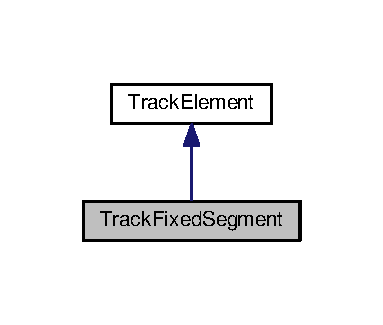
\includegraphics[width=184pt]{classKite_1_1TrackFixedSegment__inherit__graph}
\end{center}
\end{figure}
\subsubsection*{Public Member Functions}
\begin{DoxyCompactItemize}
\item 
virtual bool \hyperlink{classKite_1_1TrackFixedSegment_a21b9cefd33ae22e4c2070ad441bdd30b}{is\+Horizontal} () const
\item 
virtual bool \hyperlink{classKite_1_1TrackFixedSegment_abd54544ef1710ee4b67cfb021d73446c}{is\+Vertical} () const
\item 
virtual bool \hyperlink{classKite_1_1TrackFixedSegment_afd7362b850709bed8b61c1aa22399f97}{is\+Fixed} () const
\item 
virtual unsigned long \hyperlink{classKite_1_1TrackFixedSegment_afdedcef127ad2a3677a5b48d7d3453f3}{get\+Id} () const
\item 
virtual unsigned int \hyperlink{classKite_1_1TrackFixedSegment_a0dd7cf705ace42c662c289955313b2e9}{get\+Direction} () const
\item 
virtual \textbf{ Net} $\ast$ \hyperlink{classKite_1_1TrackFixedSegment_a692492374623a5c6096b2c4a51190359}{get\+Net} () const
\item 
virtual const \textbf{ Layer} $\ast$ \hyperlink{classKite_1_1TrackFixedSegment_ab045567c4f529dca7790d66c17c3084f}{get\+Layer} () const
\item 
virtual \hyperlink{classKite_1_1TrackElement}{Track\+Element} $\ast$ \hyperlink{classKite_1_1TrackFixedSegment_a010b7fc8801c5b88aefa4137cf85186d}{get\+Next} () const
\item 
virtual \hyperlink{classKite_1_1TrackElement}{Track\+Element} $\ast$ \hyperlink{classKite_1_1TrackFixedSegment_a55d6115d84c11ad147f4c38fe372ea24}{get\+Previous} () const
\item 
virtual \textbf{ Db\+U\+::\+Unit} \hyperlink{classKite_1_1TrackFixedSegment_ab5b5aaa5b318369feee6003dbad039c2}{get\+Axis} () const
\item 
virtual \textbf{ Interval} \hyperlink{classKite_1_1TrackFixedSegment_a034711e2d3617ea848ef9f5a18255e10}{get\+Free\+Interval} () const
\end{DoxyCompactItemize}
\subsubsection*{Static Public Member Functions}
\begin{DoxyCompactItemize}
\item 
static \hyperlink{classKite_1_1TrackElement}{Track\+Element} $\ast$ \hyperlink{classKite_1_1TrackFixedSegment_a7b548c2078a8d380b37ca12a96aa979d}{create} (\hyperlink{classKite_1_1Track}{Kite\+::\+Track} $\ast$track, \textbf{ Segment} $\ast$segment)
\end{DoxyCompactItemize}


\subsubsection{Detailed Description}
\hyperlink{classKite_1_1Track}{Track} elements for fixed wires. 

A \hyperlink{classKite_1_1TrackFixedSegment}{Track\+Fixed\+Segment} is a segment that cannot be moved from the track. It can be associated to a true blockage Segment (recognised by the fact that their owner net is the {\itshape blockage} net), or to a segment from an ordinary net but which is locked into position. In the latter case, the owned net may reuse this portion of the track if it needs it.

In all cases, the blockage ratio of the G\+Cells underneath the segment are updated. 

\subsubsection{Member Function Documentation}
\mbox{\Hypertarget{classKite_1_1TrackFixedSegment_a7b548c2078a8d380b37ca12a96aa979d}\label{classKite_1_1TrackFixedSegment_a7b548c2078a8d380b37ca12a96aa979d}} 
\index{Kite\+::\+Track\+Fixed\+Segment@{Kite\+::\+Track\+Fixed\+Segment}!create@{create}}
\index{create@{create}!Kite\+::\+Track\+Fixed\+Segment@{Kite\+::\+Track\+Fixed\+Segment}}
\paragraph{\texorpdfstring{create()}{create()}}
{\footnotesize\ttfamily \hyperlink{classKite_1_1TrackSegment}{Track\+Segment} $\ast$ create (\begin{DoxyParamCaption}\item[{\hyperlink{classKite_1_1Track}{Kite\+::\+Track} $\ast$}]{track,  }\item[{\textbf{ Segment} $\ast$}]{segment }\end{DoxyParamCaption})\hspace{0.3cm}{\ttfamily [static]}}


\begin{DoxyParams}{Parameters}
{\em segment} & The Hurricane Segment (blockage) to take into account. \\
\hline
{\em track} & A \hyperlink{classKite_1_1Track}{Track} into which insert the \hyperlink{classKite_1_1TrackFixedSegment}{Track\+Fixed\+Segment}. \\
\hline
\end{DoxyParams}
\begin{DoxyReturn}{Returns}
A \hyperlink{classKite_1_1TrackFixedSegment}{Track\+Fixed\+Segment} wrapped around a blockage Segment.
\end{DoxyReturn}
Public constructor to insert blockage inside a \hyperlink{classKite_1_1Track}{Track}. \mbox{\Hypertarget{classKite_1_1TrackFixedSegment_a21b9cefd33ae22e4c2070ad441bdd30b}\label{classKite_1_1TrackFixedSegment_a21b9cefd33ae22e4c2070ad441bdd30b}} 
\index{Kite\+::\+Track\+Fixed\+Segment@{Kite\+::\+Track\+Fixed\+Segment}!is\+Horizontal@{is\+Horizontal}}
\index{is\+Horizontal@{is\+Horizontal}!Kite\+::\+Track\+Fixed\+Segment@{Kite\+::\+Track\+Fixed\+Segment}}
\paragraph{\texorpdfstring{is\+Horizontal()}{isHorizontal()}}
{\footnotesize\ttfamily bool is\+Horizontal (\begin{DoxyParamCaption}{ }\end{DoxyParamCaption}) const\hspace{0.3cm}{\ttfamily [virtual]}}

{\bfseries See also\+:}~ \textbf{ Katabatic\+::\+Auto\+Segment\+::is\+Horizontal()}. 

Implements \hyperlink{classKite_1_1TrackElement_a9d3db1f8a5aca58f8f54d291faebf873}{Track\+Element}.

\mbox{\Hypertarget{classKite_1_1TrackFixedSegment_abd54544ef1710ee4b67cfb021d73446c}\label{classKite_1_1TrackFixedSegment_abd54544ef1710ee4b67cfb021d73446c}} 
\index{Kite\+::\+Track\+Fixed\+Segment@{Kite\+::\+Track\+Fixed\+Segment}!is\+Vertical@{is\+Vertical}}
\index{is\+Vertical@{is\+Vertical}!Kite\+::\+Track\+Fixed\+Segment@{Kite\+::\+Track\+Fixed\+Segment}}
\paragraph{\texorpdfstring{is\+Vertical()}{isVertical()}}
{\footnotesize\ttfamily bool is\+Vertical (\begin{DoxyParamCaption}{ }\end{DoxyParamCaption}) const\hspace{0.3cm}{\ttfamily [virtual]}}

{\bfseries See also\+:}~ \textbf{ Katabatic\+::\+Auto\+Segment\+::is\+Vertical()}. 

Implements \hyperlink{classKite_1_1TrackElement_a6fa2bf0568a2b295dd7cd1f7207247d5}{Track\+Element}.

\mbox{\Hypertarget{classKite_1_1TrackFixedSegment_afd7362b850709bed8b61c1aa22399f97}\label{classKite_1_1TrackFixedSegment_afd7362b850709bed8b61c1aa22399f97}} 
\index{Kite\+::\+Track\+Fixed\+Segment@{Kite\+::\+Track\+Fixed\+Segment}!is\+Fixed@{is\+Fixed}}
\index{is\+Fixed@{is\+Fixed}!Kite\+::\+Track\+Fixed\+Segment@{Kite\+::\+Track\+Fixed\+Segment}}
\paragraph{\texorpdfstring{is\+Fixed()}{isFixed()}}
{\footnotesize\ttfamily bool is\+Fixed (\begin{DoxyParamCaption}{ }\end{DoxyParamCaption}) const\hspace{0.3cm}{\ttfamily [virtual]}}

{\bfseries See also\+:}~ \textbf{ Katabatic\+::\+Auto\+Segment\+::is\+Fixed()}. 

Reimplemented from \hyperlink{classKite_1_1TrackElement_afd7362b850709bed8b61c1aa22399f97}{Track\+Element}.

\mbox{\Hypertarget{classKite_1_1TrackFixedSegment_afdedcef127ad2a3677a5b48d7d3453f3}\label{classKite_1_1TrackFixedSegment_afdedcef127ad2a3677a5b48d7d3453f3}} 
\index{Kite\+::\+Track\+Fixed\+Segment@{Kite\+::\+Track\+Fixed\+Segment}!get\+Id@{get\+Id}}
\index{get\+Id@{get\+Id}!Kite\+::\+Track\+Fixed\+Segment@{Kite\+::\+Track\+Fixed\+Segment}}
\paragraph{\texorpdfstring{get\+Id()}{getId()}}
{\footnotesize\ttfamily unsigned long get\+Id (\begin{DoxyParamCaption}{ }\end{DoxyParamCaption}) const\hspace{0.3cm}{\ttfamily [virtual]}}

\begin{DoxyReturn}{Returns}
The {\ttfamily Id} of the supporting Auto\+Segment, if there is any. {\itshape Zero} otherwise. 
\end{DoxyReturn}


Reimplemented from \hyperlink{classKite_1_1TrackElement_afdedcef127ad2a3677a5b48d7d3453f3}{Track\+Element}.

\mbox{\Hypertarget{classKite_1_1TrackFixedSegment_a0dd7cf705ace42c662c289955313b2e9}\label{classKite_1_1TrackFixedSegment_a0dd7cf705ace42c662c289955313b2e9}} 
\index{Kite\+::\+Track\+Fixed\+Segment@{Kite\+::\+Track\+Fixed\+Segment}!get\+Direction@{get\+Direction}}
\index{get\+Direction@{get\+Direction}!Kite\+::\+Track\+Fixed\+Segment@{Kite\+::\+Track\+Fixed\+Segment}}
\paragraph{\texorpdfstring{get\+Direction()}{getDirection()}}
{\footnotesize\ttfamily unsigned int get\+Direction (\begin{DoxyParamCaption}{ }\end{DoxyParamCaption}) const\hspace{0.3cm}{\ttfamily [virtual]}}

\begin{DoxyReturn}{Returns}
The direction of the supporting element (should match the preferred direction of the \hyperlink{classKite_1_1Track}{Track}). 
\end{DoxyReturn}


Implements \hyperlink{classKite_1_1TrackElement_ae35b78590ed6aa546b626ef95f28c533}{Track\+Element}.

\mbox{\Hypertarget{classKite_1_1TrackFixedSegment_a692492374623a5c6096b2c4a51190359}\label{classKite_1_1TrackFixedSegment_a692492374623a5c6096b2c4a51190359}} 
\index{Kite\+::\+Track\+Fixed\+Segment@{Kite\+::\+Track\+Fixed\+Segment}!get\+Net@{get\+Net}}
\index{get\+Net@{get\+Net}!Kite\+::\+Track\+Fixed\+Segment@{Kite\+::\+Track\+Fixed\+Segment}}
\paragraph{\texorpdfstring{get\+Net()}{getNet()}}
{\footnotesize\ttfamily \textbf{ Net} $\ast$ get\+Net (\begin{DoxyParamCaption}{ }\end{DoxyParamCaption}) const\hspace{0.3cm}{\ttfamily [virtual]}}

{\bfseries Returns\+:} The Net associated to the element (may be {\ttfamily N\+U\+LL}). 

Implements \hyperlink{classKite_1_1TrackElement_a2b383a5b6f5028911a35e446a682dabd}{Track\+Element}.

\mbox{\Hypertarget{classKite_1_1TrackFixedSegment_ab045567c4f529dca7790d66c17c3084f}\label{classKite_1_1TrackFixedSegment_ab045567c4f529dca7790d66c17c3084f}} 
\index{Kite\+::\+Track\+Fixed\+Segment@{Kite\+::\+Track\+Fixed\+Segment}!get\+Layer@{get\+Layer}}
\index{get\+Layer@{get\+Layer}!Kite\+::\+Track\+Fixed\+Segment@{Kite\+::\+Track\+Fixed\+Segment}}
\paragraph{\texorpdfstring{get\+Layer()}{getLayer()}}
{\footnotesize\ttfamily const \textbf{ Layer} $\ast$ get\+Layer (\begin{DoxyParamCaption}{ }\end{DoxyParamCaption}) const\hspace{0.3cm}{\ttfamily [virtual]}}

{\bfseries Returns\+:} The Layer of the element (should match the one of the \hyperlink{classKite_1_1Track}{Track}). 

Implements \hyperlink{classKite_1_1TrackElement_ad96c66549598873bf68c2e18ec7164c1}{Track\+Element}.

\mbox{\Hypertarget{classKite_1_1TrackFixedSegment_a010b7fc8801c5b88aefa4137cf85186d}\label{classKite_1_1TrackFixedSegment_a010b7fc8801c5b88aefa4137cf85186d}} 
\index{Kite\+::\+Track\+Fixed\+Segment@{Kite\+::\+Track\+Fixed\+Segment}!get\+Next@{get\+Next}}
\index{get\+Next@{get\+Next}!Kite\+::\+Track\+Fixed\+Segment@{Kite\+::\+Track\+Fixed\+Segment}}
\paragraph{\texorpdfstring{get\+Next()}{getNext()}}
{\footnotesize\ttfamily \hyperlink{classKite_1_1TrackElement}{Track\+Element} $\ast$ get\+Next (\begin{DoxyParamCaption}{ }\end{DoxyParamCaption}) const\hspace{0.3cm}{\ttfamily [virtual]}}

{\bfseries Returns\+:} The next \hyperlink{classKite_1_1TrackElement}{Track\+Element}, on the same track and of a {\itshape different} net. {\bfseries See also\+:}~ \hyperlink{classKite_1_1Track_af3db59591bef3c690ace92c114a4e4aa}{Track\+::get\+Next()}. 

Reimplemented from \hyperlink{classKite_1_1TrackElement_a010b7fc8801c5b88aefa4137cf85186d}{Track\+Element}.

\mbox{\Hypertarget{classKite_1_1TrackFixedSegment_a55d6115d84c11ad147f4c38fe372ea24}\label{classKite_1_1TrackFixedSegment_a55d6115d84c11ad147f4c38fe372ea24}} 
\index{Kite\+::\+Track\+Fixed\+Segment@{Kite\+::\+Track\+Fixed\+Segment}!get\+Previous@{get\+Previous}}
\index{get\+Previous@{get\+Previous}!Kite\+::\+Track\+Fixed\+Segment@{Kite\+::\+Track\+Fixed\+Segment}}
\paragraph{\texorpdfstring{get\+Previous()}{getPrevious()}}
{\footnotesize\ttfamily \hyperlink{classKite_1_1TrackElement}{Track\+Element} $\ast$ get\+Previous (\begin{DoxyParamCaption}{ }\end{DoxyParamCaption}) const\hspace{0.3cm}{\ttfamily [virtual]}}

{\bfseries Returns\+:} The previous \hyperlink{classKite_1_1TrackElement}{Track\+Element}, on the same track and of a {\itshape different} net. {\bfseries See also\+:}~ \hyperlink{classKite_1_1Track_a290fcfe6131730d216951a3b5207d777}{Track\+::get\+Previous()}. 

Reimplemented from \hyperlink{classKite_1_1TrackElement_a55d6115d84c11ad147f4c38fe372ea24}{Track\+Element}.

\mbox{\Hypertarget{classKite_1_1TrackFixedSegment_ab5b5aaa5b318369feee6003dbad039c2}\label{classKite_1_1TrackFixedSegment_ab5b5aaa5b318369feee6003dbad039c2}} 
\index{Kite\+::\+Track\+Fixed\+Segment@{Kite\+::\+Track\+Fixed\+Segment}!get\+Axis@{get\+Axis}}
\index{get\+Axis@{get\+Axis}!Kite\+::\+Track\+Fixed\+Segment@{Kite\+::\+Track\+Fixed\+Segment}}
\paragraph{\texorpdfstring{get\+Axis()}{getAxis()}}
{\footnotesize\ttfamily \textbf{ Db\+U\+::\+Unit} get\+Axis (\begin{DoxyParamCaption}{ }\end{DoxyParamCaption}) const\hspace{0.3cm}{\ttfamily [virtual]}}

{\bfseries Returns\+:} The axis position of the element (must be the same as the \hyperlink{classKite_1_1Track}{Track}). 

Implements \hyperlink{classKite_1_1TrackElement_ac492fb5399691d81c31547db6b56fd03}{Track\+Element}.

\mbox{\Hypertarget{classKite_1_1TrackFixedSegment_a034711e2d3617ea848ef9f5a18255e10}\label{classKite_1_1TrackFixedSegment_a034711e2d3617ea848ef9f5a18255e10}} 
\index{Kite\+::\+Track\+Fixed\+Segment@{Kite\+::\+Track\+Fixed\+Segment}!get\+Free\+Interval@{get\+Free\+Interval}}
\index{get\+Free\+Interval@{get\+Free\+Interval}!Kite\+::\+Track\+Fixed\+Segment@{Kite\+::\+Track\+Fixed\+Segment}}
\paragraph{\texorpdfstring{get\+Free\+Interval()}{getFreeInterval()}}
{\footnotesize\ttfamily \textbf{ Interval} get\+Free\+Interval (\begin{DoxyParamCaption}{ }\end{DoxyParamCaption}) const\hspace{0.3cm}{\ttfamily [virtual]}}

{\bfseries Returns\+:} The greatest free interval enclosing this element. 

Reimplemented from \hyperlink{classKite_1_1TrackElement_a034711e2d3617ea848ef9f5a18255e10}{Track\+Element}.



The documentation for this class was generated from the following files\+:\begin{DoxyCompactItemize}
\item 
Track\+Fixed\+Segment.\+h\item 
Track\+Fixed\+Segment.\+cpp\item 
Track\+Fixed\+Segment.\+dox\end{DoxyCompactItemize}

\hypertarget{classKite_1_1TrackMarker}{}\subsection{Track\+Marker Class Reference}
\label{classKite_1_1TrackMarker}\index{Track\+Marker@{Track\+Marker}}


Tag part of \hyperlink{classKite_1_1Track}{Track} with a weight.  


\subsubsection*{Public Member Functions}
\begin{DoxyCompactItemize}
\item 
\textbf{ Net} $\ast$ \hyperlink{classKite_1_1TrackMarker_a692492374623a5c6096b2c4a51190359}{get\+Net} () const
\item 
\textbf{ Db\+U\+::\+Unit} \hyperlink{classKite_1_1TrackMarker_ad521ffba761b0e81b7b81b99d62f76f9}{get\+SourceU} () const
\item 
\textbf{ Db\+U\+::\+Unit} \hyperlink{classKite_1_1TrackMarker_a4d52a506cd19dfa8e22e1dc0695bd960}{get\+TargetU} () const
\item 
\hyperlink{classKite_1_1Track}{Track} $\ast$ \hyperlink{classKite_1_1TrackMarker_a3f34f9139b8491a0adb531ac3a904171}{get\+Track} () const
\item 
unsigned int \hyperlink{classKite_1_1TrackMarker_a26d951691a2c0f564a4ae842ba200ea5}{get\+Weight} (const \hyperlink{classKite_1_1Track}{Track} $\ast$) const
\item 
void \hyperlink{classKite_1_1TrackMarker_abd3d8093f871d3d1a7f24b053648026c}{set\+Track} (\hyperlink{classKite_1_1Track}{Track} $\ast$)
\end{DoxyCompactItemize}
\subsubsection*{Static Public Member Functions}
\begin{DoxyCompactItemize}
\item 
static \hyperlink{classKite_1_1TrackMarker}{Track\+Marker} $\ast$ \hyperlink{classKite_1_1TrackMarker_ab44a3705a23cba53cf68357de5673c04}{create} (\textbf{ Routing\+Pad} $\ast$, size\+\_\+t depth)
\end{DoxyCompactItemize}


\subsubsection{Detailed Description}
Tag part of \hyperlink{classKite_1_1Track}{Track} with a weight. 

Track\+Markers are used to assign a cost on a span of \hyperlink{classKite_1_1Track}{Track} telling how strongly a terminal is dependant on that \hyperlink{classKite_1_1Track}{Track} to be accessed. The more \hyperlink{classKite_1_1Track}{Track} a terminal crosses, the less the weight is.

The weight is expressed in hundreth (can also be understood as percentage) of dependency over the \hyperlink{classKite_1_1Track}{Track}. As example, if a terminal can only be accessed trough one \hyperlink{classKite_1_1Track}{Track} is weight on it will be {\ttfamily 100}. 

\subsubsection{Member Function Documentation}
\mbox{\Hypertarget{classKite_1_1TrackMarker_ab44a3705a23cba53cf68357de5673c04}\label{classKite_1_1TrackMarker_ab44a3705a23cba53cf68357de5673c04}} 
\index{Kite\+::\+Track\+Marker@{Kite\+::\+Track\+Marker}!create@{create}}
\index{create@{create}!Kite\+::\+Track\+Marker@{Kite\+::\+Track\+Marker}}
\paragraph{\texorpdfstring{create()}{create()}}
{\footnotesize\ttfamily create (\begin{DoxyParamCaption}\item[{\textbf{ Routing\+Pad} $\ast$}]{rp,  }\item[{size\+\_\+t}]{depth }\end{DoxyParamCaption})\hspace{0.3cm}{\ttfamily [static]}}


\begin{DoxyParams}{Parameters}
{\em rp} & The Routing\+Pad to be accessed. \\
\hline
{\em depth} & Select the layer depth by which we want to access the Routing\+Pad. \\
\hline
\end{DoxyParams}
\begin{DoxyReturn}{Returns}
The newly created \hyperlink{classKite_1_1TrackMarker}{Track\+Marker}.
\end{DoxyReturn}
This constructor automatically take care of inserting the \hyperlink{classKite_1_1TrackMarker}{Track\+Marker} in the relevant Tracks, so it must be called during a \hyperlink{classKite_1_1Session}{Session}. \mbox{\Hypertarget{classKite_1_1TrackMarker_a692492374623a5c6096b2c4a51190359}\label{classKite_1_1TrackMarker_a692492374623a5c6096b2c4a51190359}} 
\index{Kite\+::\+Track\+Marker@{Kite\+::\+Track\+Marker}!get\+Net@{get\+Net}}
\index{get\+Net@{get\+Net}!Kite\+::\+Track\+Marker@{Kite\+::\+Track\+Marker}}
\paragraph{\texorpdfstring{get\+Net()}{getNet()}}
{\footnotesize\ttfamily \textbf{ Net} $\ast$ get\+Net (\begin{DoxyParamCaption}{ }\end{DoxyParamCaption}) const}

{\bfseries Returns\+:} The net of the Routing\+Pad. 

Referenced by Track\+Segment\+::get\+Free\+Interval(), Track\+Segment\+::get\+Next(), and Track\+Segment\+::get\+Previous().

\mbox{\Hypertarget{classKite_1_1TrackMarker_ad521ffba761b0e81b7b81b99d62f76f9}\label{classKite_1_1TrackMarker_ad521ffba761b0e81b7b81b99d62f76f9}} 
\index{Kite\+::\+Track\+Marker@{Kite\+::\+Track\+Marker}!get\+SourceU@{get\+SourceU}}
\index{get\+SourceU@{get\+SourceU}!Kite\+::\+Track\+Marker@{Kite\+::\+Track\+Marker}}
\paragraph{\texorpdfstring{get\+Source\+U()}{getSourceU()}}
{\footnotesize\ttfamily \textbf{ Db\+U\+::\+Unit} get\+SourceU (\begin{DoxyParamCaption}{ }\end{DoxyParamCaption}) const\hspace{0.3cm}{\ttfamily [inline]}}

{\bfseries Returns\+:} The span minimum bound. 

Referenced by Track\+Segment\+::\+\_\+check(), and Track\+Marker\+::set\+Track().

\mbox{\Hypertarget{classKite_1_1TrackMarker_a4d52a506cd19dfa8e22e1dc0695bd960}\label{classKite_1_1TrackMarker_a4d52a506cd19dfa8e22e1dc0695bd960}} 
\index{Kite\+::\+Track\+Marker@{Kite\+::\+Track\+Marker}!get\+TargetU@{get\+TargetU}}
\index{get\+TargetU@{get\+TargetU}!Kite\+::\+Track\+Marker@{Kite\+::\+Track\+Marker}}
\paragraph{\texorpdfstring{get\+Target\+U()}{getTargetU()}}
{\footnotesize\ttfamily \textbf{ Db\+U\+::\+Unit} get\+TargetU (\begin{DoxyParamCaption}{ }\end{DoxyParamCaption}) const\hspace{0.3cm}{\ttfamily [inline]}}

{\bfseries Returns\+:} The span maximum bound. 

Referenced by Track\+Segment\+::\+\_\+check().

\mbox{\Hypertarget{classKite_1_1TrackMarker_a3f34f9139b8491a0adb531ac3a904171}\label{classKite_1_1TrackMarker_a3f34f9139b8491a0adb531ac3a904171}} 
\index{Kite\+::\+Track\+Marker@{Kite\+::\+Track\+Marker}!get\+Track@{get\+Track}}
\index{get\+Track@{get\+Track}!Kite\+::\+Track\+Marker@{Kite\+::\+Track\+Marker}}
\paragraph{\texorpdfstring{get\+Track()}{getTrack()}}
{\footnotesize\ttfamily \hyperlink{classKite_1_1Track}{Track} $\ast$ get\+Track (\begin{DoxyParamCaption}{ }\end{DoxyParamCaption}) const\hspace{0.3cm}{\ttfamily [inline]}}

{\bfseries Returns\+:} The \hyperlink{classKite_1_1Track}{Track} into which the marker is inserted. 

Referenced by Track\+Segment\+::swap\+Track().

\mbox{\Hypertarget{classKite_1_1TrackMarker_a26d951691a2c0f564a4ae842ba200ea5}\label{classKite_1_1TrackMarker_a26d951691a2c0f564a4ae842ba200ea5}} 
\index{Kite\+::\+Track\+Marker@{Kite\+::\+Track\+Marker}!get\+Weight@{get\+Weight}}
\index{get\+Weight@{get\+Weight}!Kite\+::\+Track\+Marker@{Kite\+::\+Track\+Marker}}
\paragraph{\texorpdfstring{get\+Weight()}{getWeight()}}
{\footnotesize\ttfamily unsigned int get\+Weight (\begin{DoxyParamCaption}\item[{const \hyperlink{classKite_1_1Track}{Track} $\ast$}]{track }\end{DoxyParamCaption}) const\hspace{0.3cm}{\ttfamily [inline]}}

{\bfseries Returns\+:} The associated weight, for now the \hyperlink{classKite_1_1Track}{Track} argument is ignored. \mbox{\Hypertarget{classKite_1_1TrackMarker_abd3d8093f871d3d1a7f24b053648026c}\label{classKite_1_1TrackMarker_abd3d8093f871d3d1a7f24b053648026c}} 
\index{Kite\+::\+Track\+Marker@{Kite\+::\+Track\+Marker}!set\+Track@{set\+Track}}
\index{set\+Track@{set\+Track}!Kite\+::\+Track\+Marker@{Kite\+::\+Track\+Marker}}
\paragraph{\texorpdfstring{set\+Track()}{setTrack()}}
{\footnotesize\ttfamily void set\+Track (\begin{DoxyParamCaption}\item[{\hyperlink{classKite_1_1Track}{Track} $\ast$}]{track }\end{DoxyParamCaption})\hspace{0.3cm}{\ttfamily [inline]}}

Sets the owning \hyperlink{classKite_1_1Track}{Track}. 

Referenced by Track\+Segment\+::detach(), and Track\+Segment\+::swap\+Track().



The documentation for this class was generated from the following files\+:\begin{DoxyCompactItemize}
\item 
Track\+Marker.\+h\item 
Track\+Marker.\+cpp\item 
Track\+Marker.\+dox\end{DoxyCompactItemize}

\hypertarget{classKite_1_1TrackSegment}{}\subsection{Track\+Segment Class Reference}
\label{classKite_1_1TrackSegment}\index{Track\+Segment@{Track\+Segment}}


Derived \textbf{ Katabatic\+::\+Auto\+Segment} for the router.  




Inheritance diagram for Track\+Segment\+:\nopagebreak
\begin{figure}[H]
\begin{center}
\leavevmode
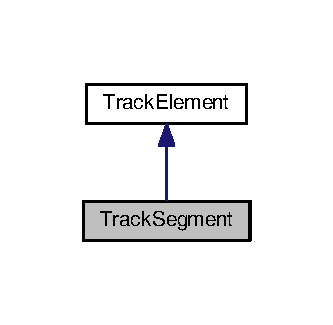
\includegraphics[width=166pt]{classKite_1_1TrackSegment__inherit__graph}
\end{center}
\end{figure}
\subsubsection*{Public Member Functions}
\begin{DoxyCompactItemize}
\item 
virtual bool \mbox{\hyperlink{classKite_1_1TrackSegment_afd7362b850709bed8b61c1aa22399f97}{is\+Fixed}} () const
\item 
virtual bool \mbox{\hyperlink{classKite_1_1TrackSegment_a21b9cefd33ae22e4c2070ad441bdd30b}{is\+Horizontal}} () const
\item 
virtual bool \mbox{\hyperlink{classKite_1_1TrackSegment_abd54544ef1710ee4b67cfb021d73446c}{is\+Vertical}} () const
\item 
virtual bool \mbox{\hyperlink{classKite_1_1TrackSegment_add556a145a89fdbcea82346abfb873dc}{is\+Local}} () const
\item 
virtual bool \mbox{\hyperlink{classKite_1_1TrackSegment_a19ba379112d6b29faa45c5eefbf38500}{is\+Global}} () const
\item 
virtual bool \mbox{\hyperlink{classKite_1_1TrackSegment_a72741158d19af38e84c5e9c08f91270f}{is\+Bipoint}} () const
\item 
virtual bool \mbox{\hyperlink{classKite_1_1TrackSegment_a1e074cb3064037035548e5e6d238e315}{is\+Terminal}} () const
\item 
virtual bool \mbox{\hyperlink{classKite_1_1TrackSegment_a62d61c231cf404a814ae37665fa8164f}{is\+Strap}} () const
\item 
virtual bool \mbox{\hyperlink{classKite_1_1TrackSegment_a782cff57d3fe10e758d19ee65a06643d}{is\+Slackened}} () const
\item 
virtual bool \mbox{\hyperlink{classKite_1_1TrackSegment_a75d91371e5281dd21f60ff39ae70a3e5}{is\+Dogleg}} () const
\item 
virtual bool \mbox{\hyperlink{classKite_1_1TrackSegment_aa0bb6f1592688e942ff67e0ac318a4fd}{can\+Dogleg}} ()
\item 
virtual bool \mbox{\hyperlink{classKite_1_1TrackSegment_accb4c6a7ee2678a0cff4dbc4a7860fe1}{can\+Dogleg}} (\textbf{ Interval})
\item 
virtual bool \mbox{\hyperlink{classKite_1_1TrackSegment_a4f040cf33009e4886d401115c3bea838}{can\+Dogleg}} (\textbf{ Katabatic\+::\+G\+Cell} $\ast$, unsigned int flags=0)
\item 
virtual float \mbox{\hyperlink{classKite_1_1TrackSegment_abb61228ad7b29c19c6428902d34126f7}{get\+Max\+Under\+Density}} (unsigned int flags) const
\item 
virtual unsigned long \mbox{\hyperlink{classKite_1_1TrackSegment_afdedcef127ad2a3677a5b48d7d3453f3}{get\+Id}} () const
\item 
virtual unsigned int \mbox{\hyperlink{classKite_1_1TrackSegment_a0dd7cf705ace42c662c289955313b2e9}{get\+Direction}} () const
\item 
virtual \textbf{ Net} $\ast$ \mbox{\hyperlink{classKite_1_1TrackSegment_a692492374623a5c6096b2c4a51190359}{get\+Net}} () const
\item 
virtual const \textbf{ Layer} $\ast$ \mbox{\hyperlink{classKite_1_1TrackSegment_ab045567c4f529dca7790d66c17c3084f}{get\+Layer}} () const
\item 
virtual unsigned long \mbox{\hyperlink{classKite_1_1TrackSegment_aa7552c20cc46abcac558627b2ca341f8}{get\+Freedom\+Degree}} () const
\item 
virtual unsigned int \mbox{\hyperlink{classKite_1_1TrackSegment_add78c6f914788c549f144998caacda84}{get\+Dogleg\+Level}} () const
\item 
virtual \mbox{\hyperlink{classKite_1_1TrackElement}{Track\+Element}} $\ast$ \mbox{\hyperlink{classKite_1_1TrackSegment_a010b7fc8801c5b88aefa4137cf85186d}{get\+Next}} () const
\item 
virtual \mbox{\hyperlink{classKite_1_1TrackElement}{Track\+Element}} $\ast$ \mbox{\hyperlink{classKite_1_1TrackSegment_a55d6115d84c11ad147f4c38fe372ea24}{get\+Previous}} () const
\item 
virtual \mbox{\hyperlink{classKite_1_1TrackElement}{Track\+Element}} $\ast$ \mbox{\hyperlink{classKite_1_1TrackSegment_a95ec3b8e7e1ec87c20ee0b37bcc96df7}{get\+Parent}} () const
\item 
virtual \textbf{ Db\+U\+::\+Unit} \mbox{\hyperlink{classKite_1_1TrackSegment_ab5b5aaa5b318369feee6003dbad039c2}{get\+Axis}} () const
\item 
virtual \textbf{ Interval} \mbox{\hyperlink{classKite_1_1TrackSegment_a034711e2d3617ea848ef9f5a18255e10}{get\+Free\+Interval}} () const
\item 
virtual \textbf{ Interval} \mbox{\hyperlink{classKite_1_1TrackSegment_a48f8b54f9489da3778d85c382a483f81}{get\+Source\+Constraints}} () const
\item 
virtual \textbf{ Interval} \mbox{\hyperlink{classKite_1_1TrackSegment_a69af7d4287bc0e44c9ca2c8e6f692be9}{get\+Target\+Constraints}} () const
\item 
virtual \mbox{\hyperlink{classKite_1_1DataNegociate}{Data\+Negociate}} $\ast$ \mbox{\hyperlink{classKite_1_1TrackSegment_acd0170a05128ec4af16ecd0060c3a3b5}{get\+Data\+Negociate}} (unsigned int flags=\mbox{\hyperlink{namespaceKite_acca8fffa3182dea5f94208f454f14b47a68e917ff37d4b5cef906303181836404}{Kt\+Data\+Self}}) const
\item 
virtual \mbox{\hyperlink{classKite_1_1TrackElement}{Track\+Element}} $\ast$ \mbox{\hyperlink{classKite_1_1TrackSegment_af2d46d64cbd02bdbba53d5483d95e26d}{get\+Canonical}} (\textbf{ Interval} \&)
\item 
virtual size\+\_\+t \mbox{\hyperlink{classKite_1_1TrackSegment_af45301f76558f613ccb605a8f851080e}{get\+G\+Cells}} (Katabatic\+::\+G\+Cell\+Vector \&) const
\item 
virtual \mbox{\hyperlink{classKite_1_1TrackElement}{Track\+Element}} $\ast$ \mbox{\hyperlink{classKite_1_1TrackSegment_a7e79fbfe77f173d46b1959c41087930a}{get\+Source\+Dogleg}} ()
\item 
virtual \mbox{\hyperlink{classKite_1_1TrackElement}{Track\+Element}} $\ast$ \mbox{\hyperlink{classKite_1_1TrackSegment_aeb4e39bd925d093e6c45599433bb421c}{get\+Target\+Dogleg}} ()
\item 
virtual Track\+Elements \mbox{\hyperlink{classKite_1_1TrackSegment_aa0ba92ebf19f596537dc051c090d5736}{get\+Perpandiculars}} ()
\item 
virtual void \mbox{\hyperlink{classKite_1_1TrackSegment_abd3d8093f871d3d1a7f24b053648026c}{set\+Track}} (\mbox{\hyperlink{classKite_1_1Track}{Track}} $\ast$)
\item 
virtual void \mbox{\hyperlink{classKite_1_1TrackSegment_af5332d647c0482aa90ad7cc9b2a50f3a}{update\+Freedom\+Degree}} ()
\item 
virtual void \mbox{\hyperlink{classKite_1_1TrackSegment_a2b90319cb042b283aa5d1fdb1992f11f}{set\+Dogleg\+Level}} (unsigned int)
\item 
virtual void \mbox{\hyperlink{classKite_1_1TrackSegment_acc245ce084989d1c34816d0e61b9d510}{swap\+Track}} (\mbox{\hyperlink{classKite_1_1TrackElement}{Track\+Element}} $\ast$)
\item 
virtual void \mbox{\hyperlink{classKite_1_1TrackSegment_a0ffe603ec7d46f21f5e56ccbe84c03fb}{reschedule}} (unsigned int level)
\item 
virtual void \mbox{\hyperlink{classKite_1_1TrackSegment_ac295bade8aee589f6718dfa79edc2a34}{detach}} ()
\item 
virtual void \mbox{\hyperlink{classKite_1_1TrackSegment_a893f1101c650c08c98612515c2b1a89c}{invalidate}} ()
\item 
virtual void \mbox{\hyperlink{classKite_1_1TrackSegment_a5bd93abe1416952ace15a98dbeeed124}{revalidate}} ()
\item 
virtual void \mbox{\hyperlink{classKite_1_1TrackSegment_a262a915c38127d3722ec561b30d80f91}{set\+Axis}} (\textbf{ Db\+U\+::\+Unit}, unsigned int flags)
\item 
virtual \mbox{\hyperlink{classKite_1_1TrackElement}{Track\+Element}} $\ast$ \mbox{\hyperlink{classKite_1_1TrackSegment_a7a9637875364e84e6862de0102341715}{make\+Dogleg}} ()
\item 
virtual \mbox{\hyperlink{classKite_1_1TrackElement}{Track\+Element}} $\ast$ \mbox{\hyperlink{classKite_1_1TrackSegment_a524f1569b2f2c1a84df2fe47e84e28ed}{make\+Dogleg}} (\textbf{ Interval}, unsigned int \&flags)
\item 
virtual void \mbox{\hyperlink{classKite_1_1TrackSegment_a10a45c049d0bd7d01c7eff1c5441c7a2}{\+\_\+post\+Doglegs}} (\mbox{\hyperlink{classKite_1_1TrackElement}{Track\+Element}} $\ast$\&perpandicular, \mbox{\hyperlink{classKite_1_1TrackElement}{Track\+Element}} $\ast$\&parallel)
\item 
virtual bool \mbox{\hyperlink{classKite_1_1TrackSegment_ad79f4c6ea0fe1135b8264a29af085909}{\+\_\+check}} () const
\end{DoxyCompactItemize}
\subsubsection*{Static Public Member Functions}
\begin{DoxyCompactItemize}
\item 
static \mbox{\hyperlink{classKite_1_1TrackElement}{Track\+Element}} $\ast$ \mbox{\hyperlink{classKite_1_1TrackSegment_a536f91d468e6c2097f85169e6d790f64}{create}} (\textbf{ Auto\+Segment} $\ast$, \mbox{\hyperlink{classKite_1_1Track}{Track}} $\ast$, bool \&created)
\end{DoxyCompactItemize}


\subsubsection{Detailed Description}
Derived \textbf{ Katabatic\+::\+Auto\+Segment} for the router. 

 We create one \mbox{\hyperlink{classKite_1_1TrackSegment}{Track\+Segment}} per aligned \textbf{ Katabatic\+::\+Auto\+Segment} set, the \mbox{\hyperlink{classKite_1_1TrackSegment}{Track\+Segment}} is associated to the canonical one of the set.

To provide some speedup, the full extention of the aligned segment set is computed once and stored in the \mbox{\hyperlink{classKite_1_1TrackSegment}{Track\+Segment}} itself. The drawback beeing that whenever one segment from the aligned set has it\textquotesingle{}s extention modified, the full extention must be recomputed.\hypertarget{classKite_1_1TrackSegment_secTSLazyRevalidate}{}\subsubsection{Lazy Revalidate}\label{classKite_1_1TrackSegment_secTSLazyRevalidate}
When the \mbox{\hyperlink{classKite_1_1TrackSegment_a5bd93abe1416952ace15a98dbeeed124}{Track\+Segment\+::revalidate()}} method is called, it only update the cached size of the segment (from the Auto\+Segment set of aligneds) and the track into which it may be inserted.

The associated \mbox{\hyperlink{classKite_1_1DataNegociate}{Data\+Negociate}} and \mbox{\hyperlink{classKite_1_1RoutingEvent}{Routing\+Event}} are {\bfseries not} updated.
\begin{DoxyItemize}
\item The \mbox{\hyperlink{classKite_1_1RoutingEvent}{Routing\+Event}} will be updated when it\textquotesingle{}s key is updated, typically during a requeueing operation {\bfseries and} in the \mbox{\hyperlink{classKite_1_1SegmentFsm}{Segment\+Fsm}} constructor. This should be optimized in the future.
\item The \mbox{\hyperlink{classKite_1_1DataNegociate}{Data\+Negociate}} is updated {\itshape only} in the \mbox{\hyperlink{classKite_1_1SegmentFsm}{Segment\+Fsm}} constructor. This is the most costly of the two updates as it perform a perpandicular \& parallel connexity exploration.
\end{DoxyItemize}\hypertarget{classKite_1_1TrackSegment_secDogleg}{}\subsubsection{Dogleg Management}\label{classKite_1_1TrackSegment_secDogleg}
The basic \textbf{ Auto\+Segment\+::can\+Dogleg()} method is declined in three more dedicated methods in this class\+:
\begin{DoxyItemize}
\item \mbox{\hyperlink{classKite_1_1TrackSegment_aa0bb6f1592688e942ff67e0ac318a4fd}{Track\+Segment\+::can\+Dogleg()}}, for locals only, check if a break is possible, never break a segment more than once (to avoid fragmentation).
\item \mbox{\hyperlink{classKite_1_1TrackSegment_a4f040cf33009e4886d401115c3bea838}{Track\+Segment\+::can\+Dogleg(\+Katabatic\+::\+G\+Cell$\ast$,unsigned int flags)}} for globals, check that the segment is breakable in the desired G\+Cell. Never break twice in the first/last G\+Cell (fragmentation limitation), but may {\itshape reuse} an already existing dogleg.
\item \mbox{\hyperlink{classKite_1_1TrackSegment_accb4c6a7ee2678a0cff4dbc4a7860fe1}{Track\+Segment\+::can\+Dogleg(\+Interval)}}, for locals only, direct proxy for the Auto\+Segment method. Never allow more than one break.
\end{DoxyItemize}

{\bfseries Relationship between Auto\+Segment and \mbox{\hyperlink{classKite_1_1TrackSegment}{Track\+Segment}}}

Figure 2 below, shows an example of dogleg creation\+:
\begin{DoxyItemize}
\item At the Katabatic level, Auto\+Segment {\ttfamily id\+:12} is broken. Thus the creation of Auto\+Segments {\ttfamily id\+:20} and {\ttfamily id\+:21}. The orignal \mbox{\hyperlink{classKite_1_1TrackSegment}{Track\+Segment}} (canonical Auto\+Segment {\ttfamily id\+:10}) remains on the right side (target) of the break.
\item But, because the canonical of the former aligned Auto\+Segment set {\ttfamily }(10,11,12,13,14) was on the {\itshape right} side of the break, the new parallel \mbox{\hyperlink{classKite_1_1TrackSegment}{Track\+Segment}} will be created on the {\ttfamily left} side, associated to the newly promoted canonical Auto\+Segment {\ttfamily id\+:12}.
\end{DoxyItemize}

 The \mbox{\hyperlink{classKite_1_1TrackSegment_a10a45c049d0bd7d01c7eff1c5441c7a2}{Track\+Segment\+::\+\_\+post\+Doglegs()}} method called by all flavors of \mbox{\hyperlink{classKite_1_1TrackSegment_a7a9637875364e84e6862de0102341715}{Track\+Segment\+::make\+Dogleg()}} methods is responsible for creating new Track\+Segments for the new doglegs (there may be more than one), it also update the dogleg level and source/target dogleg flags.

{\bfseries This section is not finished.} I need to review the parent and doglevel numbering management. There seems to be a risk of infinite fragmentation as the numbering of the original segment is not increased, we should create a {\itshape break} counter separate from deepness.\hypertarget{classKite_1_1TrackSegment_secWeakGlobal}{}\subsubsection{Global, Weak Global and Local Segments}\label{classKite_1_1TrackSegment_secWeakGlobal}
There\textquotesingle{}s a slight semantic change between Katabatic and \mbox{\hyperlink{namespaceKite}{Kite}} about what is local and what is local. This is due to how we consider the intermediate status of {\itshape Weak\+Global}.

A {\ttfamily Weak\+Global} segment is a local segment which is aligned with a global (though a V\+Tee or an H\+Tee contact).

In Katabatic a local segment is one that is not {\ttfamily Global}, a local segment can be both {\ttfamily Local} and {\ttfamily Weak\+Global}.

In \mbox{\hyperlink{namespaceKite}{Kite}} a local segment is one that is neither {\ttfamily Global} or {\ttfamily Weak\+Global}. The {\ttfamily Weak\+Global} sides with {\ttfamily Global} unlike in Katabatic. 

\subsubsection{Member Function Documentation}
\mbox{\Hypertarget{classKite_1_1TrackSegment_a536f91d468e6c2097f85169e6d790f64}\label{classKite_1_1TrackSegment_a536f91d468e6c2097f85169e6d790f64}} 
\index{Kite\+::\+Track\+Segment@{Kite\+::\+Track\+Segment}!create@{create}}
\index{create@{create}!Kite\+::\+Track\+Segment@{Kite\+::\+Track\+Segment}}
\paragraph{\texorpdfstring{create()}{create()}}
{\footnotesize\ttfamily static \mbox{\hyperlink{classKite_1_1TrackSegment}{Track\+Segment}} $\ast$ create (\begin{DoxyParamCaption}\item[{\textbf{ Auto\+Segment} $\ast$}]{segment,  }\item[{\mbox{\hyperlink{classKite_1_1Track}{Track}} $\ast$}]{track,  }\item[{bool \&}]{created }\end{DoxyParamCaption})\hspace{0.3cm}{\ttfamily [static]}}


\begin{DoxyParams}{Parameters}
{\em segment} & The Katabatic Auto\+Segment to decorate. \\
\hline
{\em track} & A \mbox{\hyperlink{classKite_1_1Track}{Track}} into which insert the \mbox{\hyperlink{classKite_1_1TrackSegment}{Track\+Segment}} (may be {\ttfamily N\+U\+LL}). \\
\hline
{\em created} & This flag is sets is a new \mbox{\hyperlink{classKite_1_1TrackSegment}{Track\+Segment}} has be created. \\
\hline
\end{DoxyParams}
\begin{DoxyReturn}{Returns}
A \mbox{\hyperlink{classKite_1_1TrackSegment}{Track\+Segment}} wrapped around an Auto\+Segment.
\end{DoxyReturn}
Constructor mainly used at loading time to decorate the Katabatic data-\/base with the router attributes. 

Referenced by Negociate\+Window\+::create\+Track\+Segment().

\mbox{\Hypertarget{classKite_1_1TrackSegment_afd7362b850709bed8b61c1aa22399f97}\label{classKite_1_1TrackSegment_afd7362b850709bed8b61c1aa22399f97}} 
\index{Kite\+::\+Track\+Segment@{Kite\+::\+Track\+Segment}!is\+Fixed@{is\+Fixed}}
\index{is\+Fixed@{is\+Fixed}!Kite\+::\+Track\+Segment@{Kite\+::\+Track\+Segment}}
\paragraph{\texorpdfstring{is\+Fixed()}{isFixed()}}
{\footnotesize\ttfamily bool is\+Fixed (\begin{DoxyParamCaption}{ }\end{DoxyParamCaption}) const\hspace{0.3cm}{\ttfamily [virtual]}}

{\bfseries See also\+:}~ \textbf{ Katabatic\+::\+Auto\+Segment\+::is\+Fixed()}. 

Reimplemented from \mbox{\hyperlink{classKite_1_1TrackElement_afd7362b850709bed8b61c1aa22399f97}{Track\+Element}}.



Referenced by Track\+Segment\+::can\+Dogleg().

\mbox{\Hypertarget{classKite_1_1TrackSegment_a21b9cefd33ae22e4c2070ad441bdd30b}\label{classKite_1_1TrackSegment_a21b9cefd33ae22e4c2070ad441bdd30b}} 
\index{Kite\+::\+Track\+Segment@{Kite\+::\+Track\+Segment}!is\+Horizontal@{is\+Horizontal}}
\index{is\+Horizontal@{is\+Horizontal}!Kite\+::\+Track\+Segment@{Kite\+::\+Track\+Segment}}
\paragraph{\texorpdfstring{is\+Horizontal()}{isHorizontal()}}
{\footnotesize\ttfamily bool is\+Horizontal (\begin{DoxyParamCaption}{ }\end{DoxyParamCaption}) const\hspace{0.3cm}{\ttfamily [virtual]}}

{\bfseries See also\+:}~ \textbf{ Katabatic\+::\+Auto\+Segment\+::is\+Horizontal()}. 

Implements \mbox{\hyperlink{classKite_1_1TrackElement_a9d3db1f8a5aca58f8f54d291faebf873}{Track\+Element}}.



Referenced by Track\+Segment\+::get\+G\+Cells().

\mbox{\Hypertarget{classKite_1_1TrackSegment_abd54544ef1710ee4b67cfb021d73446c}\label{classKite_1_1TrackSegment_abd54544ef1710ee4b67cfb021d73446c}} 
\index{Kite\+::\+Track\+Segment@{Kite\+::\+Track\+Segment}!is\+Vertical@{is\+Vertical}}
\index{is\+Vertical@{is\+Vertical}!Kite\+::\+Track\+Segment@{Kite\+::\+Track\+Segment}}
\paragraph{\texorpdfstring{is\+Vertical()}{isVertical()}}
{\footnotesize\ttfamily bool is\+Vertical (\begin{DoxyParamCaption}{ }\end{DoxyParamCaption}) const\hspace{0.3cm}{\ttfamily [virtual]}}

{\bfseries See also\+:}~ \textbf{ Katabatic\+::\+Auto\+Segment\+::is\+Vertical()}. 

Implements \mbox{\hyperlink{classKite_1_1TrackElement_a6fa2bf0568a2b295dd7cd1f7207247d5}{Track\+Element}}.

\mbox{\Hypertarget{classKite_1_1TrackSegment_add556a145a89fdbcea82346abfb873dc}\label{classKite_1_1TrackSegment_add556a145a89fdbcea82346abfb873dc}} 
\index{Kite\+::\+Track\+Segment@{Kite\+::\+Track\+Segment}!is\+Local@{is\+Local}}
\index{is\+Local@{is\+Local}!Kite\+::\+Track\+Segment@{Kite\+::\+Track\+Segment}}
\paragraph{\texorpdfstring{is\+Local()}{isLocal()}}
{\footnotesize\ttfamily bool is\+Local (\begin{DoxyParamCaption}{ }\end{DoxyParamCaption}) const\hspace{0.3cm}{\ttfamily [virtual]}}

{\bfseries See also\+:}~ Katabatic\+::is\+Local(). 

Reimplemented from \mbox{\hyperlink{classKite_1_1TrackElement_add556a145a89fdbcea82346abfb873dc}{Track\+Element}}.



Referenced by Track\+Segment\+::\+\_\+post\+Doglegs(), and Track\+Segment\+::can\+Dogleg().

\mbox{\Hypertarget{classKite_1_1TrackSegment_a19ba379112d6b29faa45c5eefbf38500}\label{classKite_1_1TrackSegment_a19ba379112d6b29faa45c5eefbf38500}} 
\index{Kite\+::\+Track\+Segment@{Kite\+::\+Track\+Segment}!is\+Global@{is\+Global}}
\index{is\+Global@{is\+Global}!Kite\+::\+Track\+Segment@{Kite\+::\+Track\+Segment}}
\paragraph{\texorpdfstring{is\+Global()}{isGlobal()}}
{\footnotesize\ttfamily bool is\+Global (\begin{DoxyParamCaption}{ }\end{DoxyParamCaption}) const\hspace{0.3cm}{\ttfamily [virtual]}}

{\bfseries See also\+:}~ \textbf{ Katabatic\+::\+Auto\+Segment\+::is\+Global()}. 

Reimplemented from \mbox{\hyperlink{classKite_1_1TrackElement_a19ba379112d6b29faa45c5eefbf38500}{Track\+Element}}.

\mbox{\Hypertarget{classKite_1_1TrackSegment_a72741158d19af38e84c5e9c08f91270f}\label{classKite_1_1TrackSegment_a72741158d19af38e84c5e9c08f91270f}} 
\index{Kite\+::\+Track\+Segment@{Kite\+::\+Track\+Segment}!is\+Bipoint@{is\+Bipoint}}
\index{is\+Bipoint@{is\+Bipoint}!Kite\+::\+Track\+Segment@{Kite\+::\+Track\+Segment}}
\paragraph{\texorpdfstring{is\+Bipoint()}{isBipoint()}}
{\footnotesize\ttfamily bool is\+Bipoint (\begin{DoxyParamCaption}{ }\end{DoxyParamCaption}) const\hspace{0.3cm}{\ttfamily [virtual]}}

{\bfseries See also\+:}~ \textbf{ Katabatic\+::\+Auto\+Segment\+::is\+Bipoint()}. 

Reimplemented from \mbox{\hyperlink{classKite_1_1TrackElement_a72741158d19af38e84c5e9c08f91270f}{Track\+Element}}.

\mbox{\Hypertarget{classKite_1_1TrackSegment_a1e074cb3064037035548e5e6d238e315}\label{classKite_1_1TrackSegment_a1e074cb3064037035548e5e6d238e315}} 
\index{Kite\+::\+Track\+Segment@{Kite\+::\+Track\+Segment}!is\+Terminal@{is\+Terminal}}
\index{is\+Terminal@{is\+Terminal}!Kite\+::\+Track\+Segment@{Kite\+::\+Track\+Segment}}
\paragraph{\texorpdfstring{is\+Terminal()}{isTerminal()}}
{\footnotesize\ttfamily bool is\+Terminal (\begin{DoxyParamCaption}{ }\end{DoxyParamCaption}) const\hspace{0.3cm}{\ttfamily [virtual]}}

{\bfseries See also\+:}~ Katabatic\+::\+Auto\+Segment\+::is\+Terminal(). 

Reimplemented from \mbox{\hyperlink{classKite_1_1TrackElement_a1e074cb3064037035548e5e6d238e315}{Track\+Element}}.

\mbox{\Hypertarget{classKite_1_1TrackSegment_a62d61c231cf404a814ae37665fa8164f}\label{classKite_1_1TrackSegment_a62d61c231cf404a814ae37665fa8164f}} 
\index{Kite\+::\+Track\+Segment@{Kite\+::\+Track\+Segment}!is\+Strap@{is\+Strap}}
\index{is\+Strap@{is\+Strap}!Kite\+::\+Track\+Segment@{Kite\+::\+Track\+Segment}}
\paragraph{\texorpdfstring{is\+Strap()}{isStrap()}}
{\footnotesize\ttfamily bool is\+Strap (\begin{DoxyParamCaption}{ }\end{DoxyParamCaption}) const\hspace{0.3cm}{\ttfamily [virtual]}}

{\bfseries See also\+:}~ \textbf{ Katabatic\+::\+Auto\+Segment\+::is\+Strap()}. 

Reimplemented from \mbox{\hyperlink{classKite_1_1TrackElement_a62d61c231cf404a814ae37665fa8164f}{Track\+Element}}.

\mbox{\Hypertarget{classKite_1_1TrackSegment_a782cff57d3fe10e758d19ee65a06643d}\label{classKite_1_1TrackSegment_a782cff57d3fe10e758d19ee65a06643d}} 
\index{Kite\+::\+Track\+Segment@{Kite\+::\+Track\+Segment}!is\+Slackened@{is\+Slackened}}
\index{is\+Slackened@{is\+Slackened}!Kite\+::\+Track\+Segment@{Kite\+::\+Track\+Segment}}
\paragraph{\texorpdfstring{is\+Slackened()}{isSlackened()}}
{\footnotesize\ttfamily bool is\+Slackened (\begin{DoxyParamCaption}{ }\end{DoxyParamCaption}) const\hspace{0.3cm}{\ttfamily [virtual]}}

{\bfseries See also\+:}~ \textbf{ Katabatic\+::\+Auto\+Segment\+::is\+Slackened()}. 

Reimplemented from \mbox{\hyperlink{classKite_1_1TrackElement_a782cff57d3fe10e758d19ee65a06643d}{Track\+Element}}.



Referenced by Track\+Segment\+::can\+Dogleg().

\mbox{\Hypertarget{classKite_1_1TrackSegment_a75d91371e5281dd21f60ff39ae70a3e5}\label{classKite_1_1TrackSegment_a75d91371e5281dd21f60ff39ae70a3e5}} 
\index{Kite\+::\+Track\+Segment@{Kite\+::\+Track\+Segment}!is\+Dogleg@{is\+Dogleg}}
\index{is\+Dogleg@{is\+Dogleg}!Kite\+::\+Track\+Segment@{Kite\+::\+Track\+Segment}}
\paragraph{\texorpdfstring{is\+Dogleg()}{isDogleg()}}
{\footnotesize\ttfamily bool is\+Dogleg (\begin{DoxyParamCaption}{ }\end{DoxyParamCaption}) const\hspace{0.3cm}{\ttfamily [virtual]}}

{\bfseries See also\+:}~ Katabatic\+::is\+Dogleg(). 

Reimplemented from \mbox{\hyperlink{classKite_1_1TrackElement_a75d91371e5281dd21f60ff39ae70a3e5}{Track\+Element}}.

\mbox{\Hypertarget{classKite_1_1TrackSegment_aa0bb6f1592688e942ff67e0ac318a4fd}\label{classKite_1_1TrackSegment_aa0bb6f1592688e942ff67e0ac318a4fd}} 
\index{Kite\+::\+Track\+Segment@{Kite\+::\+Track\+Segment}!can\+Dogleg@{can\+Dogleg}}
\index{can\+Dogleg@{can\+Dogleg}!Kite\+::\+Track\+Segment@{Kite\+::\+Track\+Segment}}
\paragraph{\texorpdfstring{can\+Dogleg()}{canDogleg()}\hspace{0.1cm}{\footnotesize\ttfamily [1/3]}}
{\footnotesize\ttfamily bool can\+Dogleg (\begin{DoxyParamCaption}{ }\end{DoxyParamCaption})\hspace{0.3cm}{\ttfamily [virtual]}}

{\bfseries See also\+:}~ \textbf{ Auto\+Segment\+::can\+Dogleg()}. At \mbox{\hyperlink{namespaceKite}{Kite}} level, this variant of the method will apply only on local segments and the segment must not already have a source or target dogleg. 

Reimplemented from \mbox{\hyperlink{classKite_1_1TrackElement_aa0bb6f1592688e942ff67e0ac318a4fd}{Track\+Element}}.

\mbox{\Hypertarget{classKite_1_1TrackSegment_accb4c6a7ee2678a0cff4dbc4a7860fe1}\label{classKite_1_1TrackSegment_accb4c6a7ee2678a0cff4dbc4a7860fe1}} 
\index{Kite\+::\+Track\+Segment@{Kite\+::\+Track\+Segment}!can\+Dogleg@{can\+Dogleg}}
\index{can\+Dogleg@{can\+Dogleg}!Kite\+::\+Track\+Segment@{Kite\+::\+Track\+Segment}}
\paragraph{\texorpdfstring{can\+Dogleg()}{canDogleg()}\hspace{0.1cm}{\footnotesize\ttfamily [2/3]}}
{\footnotesize\ttfamily bool can\+Dogleg (\begin{DoxyParamCaption}\item[{\textbf{ Interval}}]{ }\end{DoxyParamCaption})\hspace{0.3cm}{\ttfamily [virtual]}}

{\bfseries See also\+:}~ \textbf{ Auto\+Segment\+::can\+Dogleg()}. At \mbox{\hyperlink{namespaceKite}{Kite}} level, this variant of the method will apply only on local segments and the segment must not already have a source or target dogleg. 

Reimplemented from \mbox{\hyperlink{classKite_1_1TrackElement_accb4c6a7ee2678a0cff4dbc4a7860fe1}{Track\+Element}}.

\mbox{\Hypertarget{classKite_1_1TrackSegment_a4f040cf33009e4886d401115c3bea838}\label{classKite_1_1TrackSegment_a4f040cf33009e4886d401115c3bea838}} 
\index{Kite\+::\+Track\+Segment@{Kite\+::\+Track\+Segment}!can\+Dogleg@{can\+Dogleg}}
\index{can\+Dogleg@{can\+Dogleg}!Kite\+::\+Track\+Segment@{Kite\+::\+Track\+Segment}}
\paragraph{\texorpdfstring{can\+Dogleg()}{canDogleg()}\hspace{0.1cm}{\footnotesize\ttfamily [3/3]}}
{\footnotesize\ttfamily bool can\+Dogleg (\begin{DoxyParamCaption}\item[{\textbf{ Katabatic\+::\+G\+Cell} $\ast$}]{dogleg\+G\+Cell,  }\item[{unsigned int}]{flags = {\ttfamily 0} }\end{DoxyParamCaption})\hspace{0.3cm}{\ttfamily [virtual]}}

{\bfseries See also\+:}~ \textbf{ Auto\+Segment\+::can\+Dogleg()}. At kite level, this variant of the method is mainly targeted to global segment. For local segment it behave like \mbox{\hyperlink{classKite_1_1TrackElement_accb4c6a7ee2678a0cff4dbc4a7860fe1}{Track\+Element\+::can\+Dogleg(\+Interval)}}. For global segment, make the break in the requested G\+Cell {\ttfamily dogleg\+G\+Cell}. If it\textquotesingle{}s in the first or last G\+Cell and there is already a dogleg, allow to reuse it if {\ttfamily flags} contains \mbox{\hyperlink{namespaceKite_acca8fffa3182dea5f94208f454f14b47a766f453d6caa06490196a952762f0bb8}{Kite\+::\+Kt\+Allow\+Dogleg\+Reuse}}. 

Reimplemented from \mbox{\hyperlink{classKite_1_1TrackElement_a4f040cf33009e4886d401115c3bea838}{Track\+Element}}.

\mbox{\Hypertarget{classKite_1_1TrackSegment_abb61228ad7b29c19c6428902d34126f7}\label{classKite_1_1TrackSegment_abb61228ad7b29c19c6428902d34126f7}} 
\index{Kite\+::\+Track\+Segment@{Kite\+::\+Track\+Segment}!get\+Max\+Under\+Density@{get\+Max\+Under\+Density}}
\index{get\+Max\+Under\+Density@{get\+Max\+Under\+Density}!Kite\+::\+Track\+Segment@{Kite\+::\+Track\+Segment}}
\paragraph{\texorpdfstring{get\+Max\+Under\+Density()}{getMaxUnderDensity()}}
{\footnotesize\ttfamily float get\+Max\+Under\+Density (\begin{DoxyParamCaption}\item[{unsigned int}]{flags }\end{DoxyParamCaption}) const\hspace{0.3cm}{\ttfamily [virtual]}}

{\bfseries Returns\+:} The maximum density of all the G\+Cells under this element. 

Reimplemented from \mbox{\hyperlink{classKite_1_1TrackElement_aa34ceb4288e76357b65725ca00e56df8}{Track\+Element}}.

\mbox{\Hypertarget{classKite_1_1TrackSegment_afdedcef127ad2a3677a5b48d7d3453f3}\label{classKite_1_1TrackSegment_afdedcef127ad2a3677a5b48d7d3453f3}} 
\index{Kite\+::\+Track\+Segment@{Kite\+::\+Track\+Segment}!get\+Id@{get\+Id}}
\index{get\+Id@{get\+Id}!Kite\+::\+Track\+Segment@{Kite\+::\+Track\+Segment}}
\paragraph{\texorpdfstring{get\+Id()}{getId()}}
{\footnotesize\ttfamily unsigned long get\+Id (\begin{DoxyParamCaption}{ }\end{DoxyParamCaption}) const\hspace{0.3cm}{\ttfamily [virtual]}}

\begin{DoxyReturn}{Returns}
The {\ttfamily Id} of the supporting Auto\+Segment, if there is any. {\itshape Zero} otherwise. 
\end{DoxyReturn}


Reimplemented from \mbox{\hyperlink{classKite_1_1TrackElement_afdedcef127ad2a3677a5b48d7d3453f3}{Track\+Element}}.



Referenced by Track\+Segment\+::detach().

\mbox{\Hypertarget{classKite_1_1TrackSegment_a0dd7cf705ace42c662c289955313b2e9}\label{classKite_1_1TrackSegment_a0dd7cf705ace42c662c289955313b2e9}} 
\index{Kite\+::\+Track\+Segment@{Kite\+::\+Track\+Segment}!get\+Direction@{get\+Direction}}
\index{get\+Direction@{get\+Direction}!Kite\+::\+Track\+Segment@{Kite\+::\+Track\+Segment}}
\paragraph{\texorpdfstring{get\+Direction()}{getDirection()}}
{\footnotesize\ttfamily unsigned int get\+Direction (\begin{DoxyParamCaption}{ }\end{DoxyParamCaption}) const\hspace{0.3cm}{\ttfamily [virtual]}}

\begin{DoxyReturn}{Returns}
The direction of the supporting element (should match the preferred direction of the \mbox{\hyperlink{classKite_1_1Track}{Track}}). 
\end{DoxyReturn}


Implements \mbox{\hyperlink{classKite_1_1TrackElement_ae35b78590ed6aa546b626ef95f28c533}{Track\+Element}}.



Referenced by Track\+Segment\+::get\+Source\+Dogleg(), and Track\+Segment\+::get\+Target\+Dogleg().

\mbox{\Hypertarget{classKite_1_1TrackSegment_a692492374623a5c6096b2c4a51190359}\label{classKite_1_1TrackSegment_a692492374623a5c6096b2c4a51190359}} 
\index{Kite\+::\+Track\+Segment@{Kite\+::\+Track\+Segment}!get\+Net@{get\+Net}}
\index{get\+Net@{get\+Net}!Kite\+::\+Track\+Segment@{Kite\+::\+Track\+Segment}}
\paragraph{\texorpdfstring{get\+Net()}{getNet()}}
{\footnotesize\ttfamily \textbf{ Net} $\ast$ get\+Net (\begin{DoxyParamCaption}{ }\end{DoxyParamCaption}) const\hspace{0.3cm}{\ttfamily [virtual]}}

{\bfseries Returns\+:} The Net associated to the element (may be {\ttfamily N\+U\+LL}). 

Implements \mbox{\hyperlink{classKite_1_1TrackElement_a2b383a5b6f5028911a35e446a682dabd}{Track\+Element}}.



Referenced by Track\+Segment\+::get\+Free\+Interval(), Track\+Segment\+::get\+Next(), and Track\+Segment\+::get\+Previous().

\mbox{\Hypertarget{classKite_1_1TrackSegment_ab045567c4f529dca7790d66c17c3084f}\label{classKite_1_1TrackSegment_ab045567c4f529dca7790d66c17c3084f}} 
\index{Kite\+::\+Track\+Segment@{Kite\+::\+Track\+Segment}!get\+Layer@{get\+Layer}}
\index{get\+Layer@{get\+Layer}!Kite\+::\+Track\+Segment@{Kite\+::\+Track\+Segment}}
\paragraph{\texorpdfstring{get\+Layer()}{getLayer()}}
{\footnotesize\ttfamily const \textbf{ Layer} $\ast$ get\+Layer (\begin{DoxyParamCaption}{ }\end{DoxyParamCaption}) const\hspace{0.3cm}{\ttfamily [virtual]}}

{\bfseries Returns\+:} The Layer of the element (should match the one of the \mbox{\hyperlink{classKite_1_1Track}{Track}}). 

Implements \mbox{\hyperlink{classKite_1_1TrackElement_ad96c66549598873bf68c2e18ec7164c1}{Track\+Element}}.

\mbox{\Hypertarget{classKite_1_1TrackSegment_aa7552c20cc46abcac558627b2ca341f8}\label{classKite_1_1TrackSegment_aa7552c20cc46abcac558627b2ca341f8}} 
\index{Kite\+::\+Track\+Segment@{Kite\+::\+Track\+Segment}!get\+Freedom\+Degree@{get\+Freedom\+Degree}}
\index{get\+Freedom\+Degree@{get\+Freedom\+Degree}!Kite\+::\+Track\+Segment@{Kite\+::\+Track\+Segment}}
\paragraph{\texorpdfstring{get\+Freedom\+Degree()}{getFreedomDegree()}}
{\footnotesize\ttfamily unsigned long get\+Freedom\+Degree (\begin{DoxyParamCaption}{ }\end{DoxyParamCaption}) const\hspace{0.3cm}{\ttfamily [virtual]}}

{\bfseries Returns\+:} The degree of freedom of the element. It is used as a priority value when sorting \mbox{\hyperlink{classKite_1_1TrackElement}{Track\+Element}} (in \mbox{\hyperlink{classKite_1_1RoutingEvent}{Routing\+Event}}).

{\bfseries Returns\+:} The degree of freedom of the element. It is used as a priority value when sorting \mbox{\hyperlink{classKite_1_1TrackElement}{Track\+Element}} (in \mbox{\hyperlink{classKite_1_1RoutingEvent}{Routing\+Event}}).

Currently, it is the {\itshape slack} of the \textbf{ Katabatic\+::\+Auto\+Segment}. 

Reimplemented from \mbox{\hyperlink{classKite_1_1TrackElement_aa7552c20cc46abcac558627b2ca341f8}{Track\+Element}}.

\mbox{\Hypertarget{classKite_1_1TrackSegment_add78c6f914788c549f144998caacda84}\label{classKite_1_1TrackSegment_add78c6f914788c549f144998caacda84}} 
\index{Kite\+::\+Track\+Segment@{Kite\+::\+Track\+Segment}!get\+Dogleg\+Level@{get\+Dogleg\+Level}}
\index{get\+Dogleg\+Level@{get\+Dogleg\+Level}!Kite\+::\+Track\+Segment@{Kite\+::\+Track\+Segment}}
\paragraph{\texorpdfstring{get\+Dogleg\+Level()}{getDoglegLevel()}}
{\footnotesize\ttfamily unsigned int get\+Dogleg\+Level (\begin{DoxyParamCaption}{ }\end{DoxyParamCaption}) const\hspace{0.3cm}{\ttfamily [virtual]}}

{\bfseries Returns\+:} The deepness of the dogleg. 

Reimplemented from \mbox{\hyperlink{classKite_1_1TrackElement_add78c6f914788c549f144998caacda84}{Track\+Element}}.



Referenced by Track\+Segment\+::can\+Dogleg().

\mbox{\Hypertarget{classKite_1_1TrackSegment_a010b7fc8801c5b88aefa4137cf85186d}\label{classKite_1_1TrackSegment_a010b7fc8801c5b88aefa4137cf85186d}} 
\index{Kite\+::\+Track\+Segment@{Kite\+::\+Track\+Segment}!get\+Next@{get\+Next}}
\index{get\+Next@{get\+Next}!Kite\+::\+Track\+Segment@{Kite\+::\+Track\+Segment}}
\paragraph{\texorpdfstring{get\+Next()}{getNext()}}
{\footnotesize\ttfamily \mbox{\hyperlink{classKite_1_1TrackElement}{Track\+Element}} $\ast$ get\+Next (\begin{DoxyParamCaption}{ }\end{DoxyParamCaption}) const\hspace{0.3cm}{\ttfamily [virtual]}}

{\bfseries Returns\+:} The next \mbox{\hyperlink{classKite_1_1TrackElement}{Track\+Element}}, on the same track and of a {\itshape different} net. {\bfseries See also\+:}~ \mbox{\hyperlink{classKite_1_1Track_af3db59591bef3c690ace92c114a4e4aa}{Track\+::get\+Next()}}. 

Reimplemented from \mbox{\hyperlink{classKite_1_1TrackElement_a010b7fc8801c5b88aefa4137cf85186d}{Track\+Element}}.

\mbox{\Hypertarget{classKite_1_1TrackSegment_a55d6115d84c11ad147f4c38fe372ea24}\label{classKite_1_1TrackSegment_a55d6115d84c11ad147f4c38fe372ea24}} 
\index{Kite\+::\+Track\+Segment@{Kite\+::\+Track\+Segment}!get\+Previous@{get\+Previous}}
\index{get\+Previous@{get\+Previous}!Kite\+::\+Track\+Segment@{Kite\+::\+Track\+Segment}}
\paragraph{\texorpdfstring{get\+Previous()}{getPrevious()}}
{\footnotesize\ttfamily \mbox{\hyperlink{classKite_1_1TrackElement}{Track\+Element}} $\ast$ get\+Previous (\begin{DoxyParamCaption}{ }\end{DoxyParamCaption}) const\hspace{0.3cm}{\ttfamily [virtual]}}

{\bfseries Returns\+:} The previous \mbox{\hyperlink{classKite_1_1TrackElement}{Track\+Element}}, on the same track and of a {\itshape different} net. {\bfseries See also\+:}~ \mbox{\hyperlink{classKite_1_1Track_a290fcfe6131730d216951a3b5207d777}{Track\+::get\+Previous()}}. 

Reimplemented from \mbox{\hyperlink{classKite_1_1TrackElement_a55d6115d84c11ad147f4c38fe372ea24}{Track\+Element}}.

\mbox{\Hypertarget{classKite_1_1TrackSegment_a95ec3b8e7e1ec87c20ee0b37bcc96df7}\label{classKite_1_1TrackSegment_a95ec3b8e7e1ec87c20ee0b37bcc96df7}} 
\index{Kite\+::\+Track\+Segment@{Kite\+::\+Track\+Segment}!get\+Parent@{get\+Parent}}
\index{get\+Parent@{get\+Parent}!Kite\+::\+Track\+Segment@{Kite\+::\+Track\+Segment}}
\paragraph{\texorpdfstring{get\+Parent()}{getParent()}}
{\footnotesize\ttfamily \mbox{\hyperlink{classKite_1_1TrackElement}{Track\+Element}} $\ast$ get\+Parent (\begin{DoxyParamCaption}{ }\end{DoxyParamCaption}) const\hspace{0.3cm}{\ttfamily [virtual]}}

{\bfseries Returns\+:} The \mbox{\hyperlink{classKite_1_1TrackElement}{Track\+Element}} from which the dogleg has been created, if any. 

Reimplemented from \mbox{\hyperlink{classKite_1_1TrackElement_a95ec3b8e7e1ec87c20ee0b37bcc96df7}{Track\+Element}}.



Referenced by Track\+Segment\+::get\+Data\+Negociate().

\mbox{\Hypertarget{classKite_1_1TrackSegment_ab5b5aaa5b318369feee6003dbad039c2}\label{classKite_1_1TrackSegment_ab5b5aaa5b318369feee6003dbad039c2}} 
\index{Kite\+::\+Track\+Segment@{Kite\+::\+Track\+Segment}!get\+Axis@{get\+Axis}}
\index{get\+Axis@{get\+Axis}!Kite\+::\+Track\+Segment@{Kite\+::\+Track\+Segment}}
\paragraph{\texorpdfstring{get\+Axis()}{getAxis()}}
{\footnotesize\ttfamily \textbf{ Db\+U\+::\+Unit} get\+Axis (\begin{DoxyParamCaption}{ }\end{DoxyParamCaption}) const\hspace{0.3cm}{\ttfamily [virtual]}}

{\bfseries Returns\+:} The axis position of the element (must be the same as the \mbox{\hyperlink{classKite_1_1Track}{Track}}). 

Implements \mbox{\hyperlink{classKite_1_1TrackElement_ac492fb5399691d81c31547db6b56fd03}{Track\+Element}}.

\mbox{\Hypertarget{classKite_1_1TrackSegment_a034711e2d3617ea848ef9f5a18255e10}\label{classKite_1_1TrackSegment_a034711e2d3617ea848ef9f5a18255e10}} 
\index{Kite\+::\+Track\+Segment@{Kite\+::\+Track\+Segment}!get\+Free\+Interval@{get\+Free\+Interval}}
\index{get\+Free\+Interval@{get\+Free\+Interval}!Kite\+::\+Track\+Segment@{Kite\+::\+Track\+Segment}}
\paragraph{\texorpdfstring{get\+Free\+Interval()}{getFreeInterval()}}
{\footnotesize\ttfamily \textbf{ Interval} get\+Free\+Interval (\begin{DoxyParamCaption}{ }\end{DoxyParamCaption}) const\hspace{0.3cm}{\ttfamily [virtual]}}

{\bfseries Returns\+:} The greatest free interval enclosing this element. 

Reimplemented from \mbox{\hyperlink{classKite_1_1TrackElement_a034711e2d3617ea848ef9f5a18255e10}{Track\+Element}}.

\mbox{\Hypertarget{classKite_1_1TrackSegment_a48f8b54f9489da3778d85c382a483f81}\label{classKite_1_1TrackSegment_a48f8b54f9489da3778d85c382a483f81}} 
\index{Kite\+::\+Track\+Segment@{Kite\+::\+Track\+Segment}!get\+Source\+Constraints@{get\+Source\+Constraints}}
\index{get\+Source\+Constraints@{get\+Source\+Constraints}!Kite\+::\+Track\+Segment@{Kite\+::\+Track\+Segment}}
\paragraph{\texorpdfstring{get\+Source\+Constraints()}{getSourceConstraints()}}
{\footnotesize\ttfamily \textbf{ Interval} get\+Source\+Constraints (\begin{DoxyParamCaption}{ }\end{DoxyParamCaption}) const\hspace{0.3cm}{\ttfamily [virtual]}}

{\bfseries See also\+:}~ \textbf{ Katabatic\+::\+Auto\+Segment\+::get\+Source\+Constraints()}. 

Reimplemented from \mbox{\hyperlink{classKite_1_1TrackElement_a48f8b54f9489da3778d85c382a483f81}{Track\+Element}}.

\mbox{\Hypertarget{classKite_1_1TrackSegment_a69af7d4287bc0e44c9ca2c8e6f692be9}\label{classKite_1_1TrackSegment_a69af7d4287bc0e44c9ca2c8e6f692be9}} 
\index{Kite\+::\+Track\+Segment@{Kite\+::\+Track\+Segment}!get\+Target\+Constraints@{get\+Target\+Constraints}}
\index{get\+Target\+Constraints@{get\+Target\+Constraints}!Kite\+::\+Track\+Segment@{Kite\+::\+Track\+Segment}}
\paragraph{\texorpdfstring{get\+Target\+Constraints()}{getTargetConstraints()}}
{\footnotesize\ttfamily \textbf{ Interval} get\+Target\+Constraints (\begin{DoxyParamCaption}{ }\end{DoxyParamCaption}) const\hspace{0.3cm}{\ttfamily [virtual]}}

{\bfseries See also\+:}~ \textbf{ Katabatic\+::\+Auto\+Segment\+::get\+Target\+Constraints()}. 

Reimplemented from \mbox{\hyperlink{classKite_1_1TrackElement_a69af7d4287bc0e44c9ca2c8e6f692be9}{Track\+Element}}.

\mbox{\Hypertarget{classKite_1_1TrackSegment_acd0170a05128ec4af16ecd0060c3a3b5}\label{classKite_1_1TrackSegment_acd0170a05128ec4af16ecd0060c3a3b5}} 
\index{Kite\+::\+Track\+Segment@{Kite\+::\+Track\+Segment}!get\+Data\+Negociate@{get\+Data\+Negociate}}
\index{get\+Data\+Negociate@{get\+Data\+Negociate}!Kite\+::\+Track\+Segment@{Kite\+::\+Track\+Segment}}
\paragraph{\texorpdfstring{get\+Data\+Negociate()}{getDataNegociate()}}
{\footnotesize\ttfamily \mbox{\hyperlink{classKite_1_1DataNegociate}{Data\+Negociate}} $\ast$ get\+Data\+Negociate (\begin{DoxyParamCaption}\item[{unsigned int}]{flags = {\ttfamily \mbox{\hyperlink{namespaceKite_acca8fffa3182dea5f94208f454f14b47a68e917ff37d4b5cef906303181836404}{Kt\+Data\+Self}}} }\end{DoxyParamCaption}) const\hspace{0.3cm}{\ttfamily [virtual]}}

{\bfseries Returns\+:} The additional data-\/structure supplied by the routing algorithm. 

Reimplemented from \mbox{\hyperlink{classKite_1_1TrackElement_acd0170a05128ec4af16ecd0060c3a3b5}{Track\+Element}}.



Referenced by Track\+Segment\+::\+\_\+post\+Doglegs(), and Track\+Segment\+::swap\+Track().

\mbox{\Hypertarget{classKite_1_1TrackSegment_af2d46d64cbd02bdbba53d5483d95e26d}\label{classKite_1_1TrackSegment_af2d46d64cbd02bdbba53d5483d95e26d}} 
\index{Kite\+::\+Track\+Segment@{Kite\+::\+Track\+Segment}!get\+Canonical@{get\+Canonical}}
\index{get\+Canonical@{get\+Canonical}!Kite\+::\+Track\+Segment@{Kite\+::\+Track\+Segment}}
\paragraph{\texorpdfstring{get\+Canonical()}{getCanonical()}}
{\footnotesize\ttfamily \mbox{\hyperlink{classKite_1_1TrackElement}{Track\+Element}} $\ast$ get\+Canonical (\begin{DoxyParamCaption}\item[{\textbf{ Interval} \&}]{i }\end{DoxyParamCaption})\hspace{0.3cm}{\ttfamily [virtual]}}

Inner working still unclear to myself. 

Reimplemented from \mbox{\hyperlink{classKite_1_1TrackElement_af2d46d64cbd02bdbba53d5483d95e26d}{Track\+Element}}.

\mbox{\Hypertarget{classKite_1_1TrackSegment_af45301f76558f613ccb605a8f851080e}\label{classKite_1_1TrackSegment_af45301f76558f613ccb605a8f851080e}} 
\index{Kite\+::\+Track\+Segment@{Kite\+::\+Track\+Segment}!get\+G\+Cells@{get\+G\+Cells}}
\index{get\+G\+Cells@{get\+G\+Cells}!Kite\+::\+Track\+Segment@{Kite\+::\+Track\+Segment}}
\paragraph{\texorpdfstring{get\+G\+Cells()}{getGCells()}}
{\footnotesize\ttfamily size\+\_\+t get\+G\+Cells (\begin{DoxyParamCaption}\item[{Katabatic\+::\+G\+Cell\+Vector \&}]{gcells }\end{DoxyParamCaption}) const\hspace{0.3cm}{\ttfamily [virtual]}}

{\bfseries Returns\+:} The table of \textbf{ Katabatic\+::\+G\+Cell} underneath the element whole span. 

Reimplemented from \mbox{\hyperlink{classKite_1_1TrackElement_af45301f76558f613ccb605a8f851080e}{Track\+Element}}.



Referenced by Track\+Segment\+::can\+Dogleg().

\mbox{\Hypertarget{classKite_1_1TrackSegment_a7e79fbfe77f173d46b1959c41087930a}\label{classKite_1_1TrackSegment_a7e79fbfe77f173d46b1959c41087930a}} 
\index{Kite\+::\+Track\+Segment@{Kite\+::\+Track\+Segment}!get\+Source\+Dogleg@{get\+Source\+Dogleg}}
\index{get\+Source\+Dogleg@{get\+Source\+Dogleg}!Kite\+::\+Track\+Segment@{Kite\+::\+Track\+Segment}}
\paragraph{\texorpdfstring{get\+Source\+Dogleg()}{getSourceDogleg()}}
{\footnotesize\ttfamily \mbox{\hyperlink{classKite_1_1TrackElement}{Track\+Element}} $\ast$ get\+Source\+Dogleg (\begin{DoxyParamCaption}{ }\end{DoxyParamCaption})\hspace{0.3cm}{\ttfamily [virtual]}}

{\bfseries Returns\+:} The source part of the segment from which the dogleg has been created. 

Reimplemented from \mbox{\hyperlink{classKite_1_1TrackElement_a7e79fbfe77f173d46b1959c41087930a}{Track\+Element}}.

\mbox{\Hypertarget{classKite_1_1TrackSegment_aeb4e39bd925d093e6c45599433bb421c}\label{classKite_1_1TrackSegment_aeb4e39bd925d093e6c45599433bb421c}} 
\index{Kite\+::\+Track\+Segment@{Kite\+::\+Track\+Segment}!get\+Target\+Dogleg@{get\+Target\+Dogleg}}
\index{get\+Target\+Dogleg@{get\+Target\+Dogleg}!Kite\+::\+Track\+Segment@{Kite\+::\+Track\+Segment}}
\paragraph{\texorpdfstring{get\+Target\+Dogleg()}{getTargetDogleg()}}
{\footnotesize\ttfamily \mbox{\hyperlink{classKite_1_1TrackElement}{Track\+Element}} $\ast$ get\+Target\+Dogleg (\begin{DoxyParamCaption}{ }\end{DoxyParamCaption})\hspace{0.3cm}{\ttfamily [virtual]}}

{\bfseries Returns\+:} The target part of the segment from which the dogleg has been created. 

Reimplemented from \mbox{\hyperlink{classKite_1_1TrackElement_aeb4e39bd925d093e6c45599433bb421c}{Track\+Element}}.

\mbox{\Hypertarget{classKite_1_1TrackSegment_aa0ba92ebf19f596537dc051c090d5736}\label{classKite_1_1TrackSegment_aa0ba92ebf19f596537dc051c090d5736}} 
\index{Kite\+::\+Track\+Segment@{Kite\+::\+Track\+Segment}!get\+Perpandiculars@{get\+Perpandiculars}}
\index{get\+Perpandiculars@{get\+Perpandiculars}!Kite\+::\+Track\+Segment@{Kite\+::\+Track\+Segment}}
\paragraph{\texorpdfstring{get\+Perpandiculars()}{getPerpandiculars()}}
{\footnotesize\ttfamily Track\+Elements get\+Perpandiculars (\begin{DoxyParamCaption}{ }\end{DoxyParamCaption})\hspace{0.3cm}{\ttfamily [virtual]}}

{\bfseries Returns\+:} The collection of all element perpandiculars to this one. 

Reimplemented from \mbox{\hyperlink{classKite_1_1TrackElement_aa0ba92ebf19f596537dc051c090d5736}{Track\+Element}}.

\mbox{\Hypertarget{classKite_1_1TrackSegment_abd3d8093f871d3d1a7f24b053648026c}\label{classKite_1_1TrackSegment_abd3d8093f871d3d1a7f24b053648026c}} 
\index{Kite\+::\+Track\+Segment@{Kite\+::\+Track\+Segment}!set\+Track@{set\+Track}}
\index{set\+Track@{set\+Track}!Kite\+::\+Track\+Segment@{Kite\+::\+Track\+Segment}}
\paragraph{\texorpdfstring{set\+Track()}{setTrack()}}
{\footnotesize\ttfamily void set\+Track (\begin{DoxyParamCaption}\item[{\mbox{\hyperlink{classKite_1_1Track}{Track}} $\ast$}]{track }\end{DoxyParamCaption})\hspace{0.3cm}{\ttfamily [virtual]}}

Insert the element into {\ttfamily track}, also used as an insertion marker. 

Reimplemented from \mbox{\hyperlink{classKite_1_1TrackElement_abd3d8093f871d3d1a7f24b053648026c}{Track\+Element}}.



Referenced by Track\+Segment\+::detach(), and Track\+Segment\+::swap\+Track().

\mbox{\Hypertarget{classKite_1_1TrackSegment_af5332d647c0482aa90ad7cc9b2a50f3a}\label{classKite_1_1TrackSegment_af5332d647c0482aa90ad7cc9b2a50f3a}} 
\index{Kite\+::\+Track\+Segment@{Kite\+::\+Track\+Segment}!update\+Freedom\+Degree@{update\+Freedom\+Degree}}
\index{update\+Freedom\+Degree@{update\+Freedom\+Degree}!Kite\+::\+Track\+Segment@{Kite\+::\+Track\+Segment}}
\paragraph{\texorpdfstring{update\+Freedom\+Degree()}{updateFreedomDegree()}}
{\footnotesize\ttfamily void update\+Freedom\+Degree (\begin{DoxyParamCaption}{ }\end{DoxyParamCaption})\hspace{0.3cm}{\ttfamily [virtual]}}

Update, from the element characteristics, it\textquotesingle{}s degree of freedom. 

Reimplemented from \mbox{\hyperlink{classKite_1_1TrackElement_af5332d647c0482aa90ad7cc9b2a50f3a}{Track\+Element}}.

\mbox{\Hypertarget{classKite_1_1TrackSegment_a2b90319cb042b283aa5d1fdb1992f11f}\label{classKite_1_1TrackSegment_a2b90319cb042b283aa5d1fdb1992f11f}} 
\index{Kite\+::\+Track\+Segment@{Kite\+::\+Track\+Segment}!set\+Dogleg\+Level@{set\+Dogleg\+Level}}
\index{set\+Dogleg\+Level@{set\+Dogleg\+Level}!Kite\+::\+Track\+Segment@{Kite\+::\+Track\+Segment}}
\paragraph{\texorpdfstring{set\+Dogleg\+Level()}{setDoglegLevel()}}
{\footnotesize\ttfamily void set\+Dogleg\+Level (\begin{DoxyParamCaption}\item[{unsigned int}]{level }\end{DoxyParamCaption})\hspace{0.3cm}{\ttfamily [virtual]}}

Sets the level of dogleg of the element. 

Reimplemented from \mbox{\hyperlink{classKite_1_1TrackElement_a2b90319cb042b283aa5d1fdb1992f11f}{Track\+Element}}.

\mbox{\Hypertarget{classKite_1_1TrackSegment_acc245ce084989d1c34816d0e61b9d510}\label{classKite_1_1TrackSegment_acc245ce084989d1c34816d0e61b9d510}} 
\index{Kite\+::\+Track\+Segment@{Kite\+::\+Track\+Segment}!swap\+Track@{swap\+Track}}
\index{swap\+Track@{swap\+Track}!Kite\+::\+Track\+Segment@{Kite\+::\+Track\+Segment}}
\paragraph{\texorpdfstring{swap\+Track()}{swapTrack()}}
{\footnotesize\ttfamily void swap\+Track (\begin{DoxyParamCaption}\item[{\mbox{\hyperlink{classKite_1_1TrackElement}{Track\+Element}} $\ast$}]{other }\end{DoxyParamCaption})\hspace{0.3cm}{\ttfamily [virtual]}}

Swap the tracks of {\ttfamily this} and {\ttfamily other}. 

Reimplemented from \mbox{\hyperlink{classKite_1_1TrackElement_acc245ce084989d1c34816d0e61b9d510}{Track\+Element}}.

\mbox{\Hypertarget{classKite_1_1TrackSegment_a0ffe603ec7d46f21f5e56ccbe84c03fb}\label{classKite_1_1TrackSegment_a0ffe603ec7d46f21f5e56ccbe84c03fb}} 
\index{Kite\+::\+Track\+Segment@{Kite\+::\+Track\+Segment}!reschedule@{reschedule}}
\index{reschedule@{reschedule}!Kite\+::\+Track\+Segment@{Kite\+::\+Track\+Segment}}
\paragraph{\texorpdfstring{reschedule()}{reschedule()}}
{\footnotesize\ttfamily void reschedule (\begin{DoxyParamCaption}\item[{unsigned int}]{level }\end{DoxyParamCaption})\hspace{0.3cm}{\ttfamily [virtual]}}

If the \mbox{\hyperlink{classKite_1_1TrackElement}{Track\+Element}} has already an event scheduled, change the level of this event, otherwise create a new event.

{\bfseries See also\+:}~ Negotiate\+Window\+::reschedule\+Event(). 

Reimplemented from \mbox{\hyperlink{classKite_1_1TrackElement_a0ffe603ec7d46f21f5e56ccbe84c03fb}{Track\+Element}}.



Referenced by Track\+Segment\+::\+\_\+post\+Doglegs().

\mbox{\Hypertarget{classKite_1_1TrackSegment_ac295bade8aee589f6718dfa79edc2a34}\label{classKite_1_1TrackSegment_ac295bade8aee589f6718dfa79edc2a34}} 
\index{Kite\+::\+Track\+Segment@{Kite\+::\+Track\+Segment}!detach@{detach}}
\index{detach@{detach}!Kite\+::\+Track\+Segment@{Kite\+::\+Track\+Segment}}
\paragraph{\texorpdfstring{detach()}{detach()}}
{\footnotesize\ttfamily void detach (\begin{DoxyParamCaption}{ }\end{DoxyParamCaption})\hspace{0.3cm}{\ttfamily [virtual]}}

Remove the link from the \mbox{\hyperlink{classKite_1_1TrackElement}{Track\+Element}} to it\textquotesingle{}s owning \mbox{\hyperlink{classKite_1_1Track}{Track}}, marking it for removal. The removal from the \mbox{\hyperlink{classKite_1_1Track}{Track}}\textquotesingle{}s vector is managed by the \mbox{\hyperlink{classKite_1_1Track}{Track}} itself during the \mbox{\hyperlink{classKite_1_1Session}{Session}} revalidation stage. 

Reimplemented from \mbox{\hyperlink{classKite_1_1TrackElement_ac295bade8aee589f6718dfa79edc2a34}{Track\+Element}}.

\mbox{\Hypertarget{classKite_1_1TrackSegment_a893f1101c650c08c98612515c2b1a89c}\label{classKite_1_1TrackSegment_a893f1101c650c08c98612515c2b1a89c}} 
\index{Kite\+::\+Track\+Segment@{Kite\+::\+Track\+Segment}!invalidate@{invalidate}}
\index{invalidate@{invalidate}!Kite\+::\+Track\+Segment@{Kite\+::\+Track\+Segment}}
\paragraph{\texorpdfstring{invalidate()}{invalidate()}}
{\footnotesize\ttfamily void invalidate (\begin{DoxyParamCaption}{ }\end{DoxyParamCaption})\hspace{0.3cm}{\ttfamily [virtual]}}

{\bfseries See also\+:}~ \textbf{ Auto\+Segment\+::invalidate()}. 

Reimplemented from \mbox{\hyperlink{classKite_1_1TrackElement_a893f1101c650c08c98612515c2b1a89c}{Track\+Element}}.



Referenced by Track\+Segment\+::create(), and Track\+Segment\+::set\+Axis().

\mbox{\Hypertarget{classKite_1_1TrackSegment_a5bd93abe1416952ace15a98dbeeed124}\label{classKite_1_1TrackSegment_a5bd93abe1416952ace15a98dbeeed124}} 
\index{Kite\+::\+Track\+Segment@{Kite\+::\+Track\+Segment}!revalidate@{revalidate}}
\index{revalidate@{revalidate}!Kite\+::\+Track\+Segment@{Kite\+::\+Track\+Segment}}
\paragraph{\texorpdfstring{revalidate()}{revalidate()}}
{\footnotesize\ttfamily void revalidate (\begin{DoxyParamCaption}{ }\end{DoxyParamCaption})\hspace{0.3cm}{\ttfamily [virtual]}}

Actualize the \mbox{\hyperlink{classKite_1_1TrackSegment}{Track\+Segment}} characteristics from the supporting elements (set of Auto\+Segment).

This method do not update the \mbox{\hyperlink{classKite_1_1DataNegociate}{Data\+Negociate}} or the \mbox{\hyperlink{classKite_1_1RoutingEvent}{Routing\+Event}}. This is a lazy update delayed until the constructor of \mbox{\hyperlink{classKite_1_1SegmentFsm}{Segment\+Fsm}} is called. (see \mbox{\hyperlink{classKite_1_1TrackSegment_secTSLazyRevalidate}{Lazy Revalidate}}). 

Reimplemented from \mbox{\hyperlink{classKite_1_1TrackElement_a5bd93abe1416952ace15a98dbeeed124}{Track\+Element}}.

\mbox{\Hypertarget{classKite_1_1TrackSegment_a262a915c38127d3722ec561b30d80f91}\label{classKite_1_1TrackSegment_a262a915c38127d3722ec561b30d80f91}} 
\index{Kite\+::\+Track\+Segment@{Kite\+::\+Track\+Segment}!set\+Axis@{set\+Axis}}
\index{set\+Axis@{set\+Axis}!Kite\+::\+Track\+Segment@{Kite\+::\+Track\+Segment}}
\paragraph{\texorpdfstring{set\+Axis()}{setAxis()}}
{\footnotesize\ttfamily void set\+Axis (\begin{DoxyParamCaption}\item[{\textbf{ Db\+U\+::\+Unit}}]{,  }\item[{unsigned int}]{flags }\end{DoxyParamCaption})\hspace{0.3cm}{\ttfamily [virtual]}}

Sets the axis of the \mbox{\hyperlink{classKite_1_1TrackElement}{Track\+Element}}. 

Reimplemented from \mbox{\hyperlink{classKite_1_1TrackElement_a45e685b1e3ee630d24bf43746553af4c}{Track\+Element}}.

\mbox{\Hypertarget{classKite_1_1TrackSegment_a7a9637875364e84e6862de0102341715}\label{classKite_1_1TrackSegment_a7a9637875364e84e6862de0102341715}} 
\index{Kite\+::\+Track\+Segment@{Kite\+::\+Track\+Segment}!make\+Dogleg@{make\+Dogleg}}
\index{make\+Dogleg@{make\+Dogleg}!Kite\+::\+Track\+Segment@{Kite\+::\+Track\+Segment}}
\paragraph{\texorpdfstring{make\+Dogleg()}{makeDogleg()}\hspace{0.1cm}{\footnotesize\ttfamily [1/2]}}
{\footnotesize\ttfamily \mbox{\hyperlink{classKite_1_1TrackElement}{Track\+Element}} $\ast$ make\+Dogleg (\begin{DoxyParamCaption}{ }\end{DoxyParamCaption})\hspace{0.3cm}{\ttfamily [virtual]}}

Create a dogleg on the source end of the \mbox{\hyperlink{classKite_1_1TrackSegment}{Track\+Segment}}. Put the dogleg axis on the source {\bfseries To be further reviewed}.

{\bfseries See also\+:}~ \mbox{\hyperlink{classKite_1_1TrackSegment_secDogleg}{Dogleg management}}.

Post-\/processing done by \mbox{\hyperlink{classKite_1_1TrackSegment_a10a45c049d0bd7d01c7eff1c5441c7a2}{Track\+Segment\+::\+\_\+post\+Doglegs()}}. 

Reimplemented from \mbox{\hyperlink{classKite_1_1TrackElement_a7a9637875364e84e6862de0102341715}{Track\+Element}}.

\mbox{\Hypertarget{classKite_1_1TrackSegment_a524f1569b2f2c1a84df2fe47e84e28ed}\label{classKite_1_1TrackSegment_a524f1569b2f2c1a84df2fe47e84e28ed}} 
\index{Kite\+::\+Track\+Segment@{Kite\+::\+Track\+Segment}!make\+Dogleg@{make\+Dogleg}}
\index{make\+Dogleg@{make\+Dogleg}!Kite\+::\+Track\+Segment@{Kite\+::\+Track\+Segment}}
\paragraph{\texorpdfstring{make\+Dogleg()}{makeDogleg()}\hspace{0.1cm}{\footnotesize\ttfamily [2/2]}}
{\footnotesize\ttfamily \mbox{\hyperlink{classKite_1_1TrackElement}{Track\+Element}} $\ast$ make\+Dogleg (\begin{DoxyParamCaption}\item[{\textbf{ Interval}}]{interval,  }\item[{unsigned int \&}]{flags }\end{DoxyParamCaption})\hspace{0.3cm}{\ttfamily [virtual]}}

{\bfseries See also\+:}~ \textbf{ Auto\+Segment\+::make\+Dogleg()}, \mbox{\hyperlink{classKite_1_1TrackSegment_secDogleg}{Dogleg management}}, the return flags from this method are returned through the {\ttfamily flags} variable.

Post-\/processing done by \mbox{\hyperlink{classKite_1_1TrackSegment_a10a45c049d0bd7d01c7eff1c5441c7a2}{Track\+Segment\+::\+\_\+post\+Doglegs()}}. 

Reimplemented from \mbox{\hyperlink{classKite_1_1TrackElement_a524f1569b2f2c1a84df2fe47e84e28ed}{Track\+Element}}.

\mbox{\Hypertarget{classKite_1_1TrackSegment_a10a45c049d0bd7d01c7eff1c5441c7a2}\label{classKite_1_1TrackSegment_a10a45c049d0bd7d01c7eff1c5441c7a2}} 
\index{Kite\+::\+Track\+Segment@{Kite\+::\+Track\+Segment}!\+\_\+post\+Doglegs@{\+\_\+post\+Doglegs}}
\index{\+\_\+post\+Doglegs@{\+\_\+post\+Doglegs}!Kite\+::\+Track\+Segment@{Kite\+::\+Track\+Segment}}
\paragraph{\texorpdfstring{\+\_\+post\+Doglegs()}{\_postDoglegs()}}
{\footnotesize\ttfamily \mbox{\hyperlink{classKite_1_1TrackSegment}{Track\+Segment}} $\ast$ \+\_\+post\+Doglegs (\begin{DoxyParamCaption}\item[{\mbox{\hyperlink{classKite_1_1TrackElement}{Track\+Element}} $\ast$\&}]{perpandicular,  }\item[{\mbox{\hyperlink{classKite_1_1TrackElement}{Track\+Element}} $\ast$\&}]{parallel }\end{DoxyParamCaption})\hspace{0.3cm}{\ttfamily [virtual]}}

Post-\/process to be called inside the various dogleg creation or slacken methods. Iterate through the newly created Auto\+Segments to create, for the {\itshape perpandicular} and the {\itshape new parallel} associateds Track\+Segments. Also sets the dogleg levels and flags of the newly created elements.

The session dogleg reset is called at the end of this method. The {\ttfamily perpandicular} and {\ttfamily parallel} references to pointers contains the newly created segments for the {\bfseries last} dogleg. If more than one was created, you cannot access them (the need has not arised yet). 

Reimplemented from \mbox{\hyperlink{classKite_1_1TrackElement}{Track\+Element}}.



Referenced by Track\+Segment\+::make\+Dogleg().

\mbox{\Hypertarget{classKite_1_1TrackSegment_ad79f4c6ea0fe1135b8264a29af085909}\label{classKite_1_1TrackSegment_ad79f4c6ea0fe1135b8264a29af085909}} 
\index{Kite\+::\+Track\+Segment@{Kite\+::\+Track\+Segment}!\+\_\+check@{\+\_\+check}}
\index{\+\_\+check@{\+\_\+check}!Kite\+::\+Track\+Segment@{Kite\+::\+Track\+Segment}}
\paragraph{\texorpdfstring{\+\_\+check()}{\_check()}}
{\footnotesize\ttfamily bool \+\_\+check (\begin{DoxyParamCaption}{ }\end{DoxyParamCaption}) const\hspace{0.3cm}{\ttfamily [virtual]}}

Check the coherency of the element. For a \mbox{\hyperlink{classKite_1_1TrackSegment}{Track\+Segment}}\+:
\begin{DoxyItemize}
\item The supporting Auto\+Segment the canonical one of the set.
\item The cached {\ttfamily min} \& {\ttfamily max} values are identical to the computed ones.
\end{DoxyItemize}

{\bfseries Returns\+:} {\bfseries true} on success. 

Reimplemented from \mbox{\hyperlink{classKite_1_1TrackElement_ad79f4c6ea0fe1135b8264a29af085909}{Track\+Element}}.



The documentation for this class was generated from the following files\+:\begin{DoxyCompactItemize}
\item 
Track\+Segment.\+h\item 
Track\+Segment.\+cpp\item 
Track\+Segment.\+dox\end{DoxyCompactItemize}

\hypertarget{classKite_1_1VerticalTrack}{\subsection{Vertical\-Track Class Reference}
\label{classKite_1_1VerticalTrack}\index{Vertical\-Track@{Vertical\-Track}}
}


Vertical track managment.  




Inheritance diagram for Vertical\-Track\-:\nopagebreak
\begin{figure}[H]
\begin{center}
\leavevmode
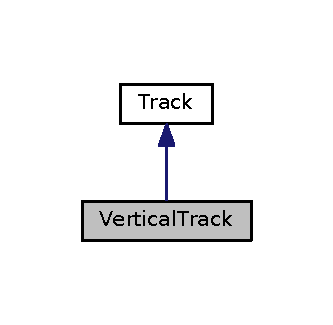
\includegraphics[width=154pt]{classKite_1_1VerticalTrack__inherit__graph}
\end{center}
\end{figure}
\subsubsection*{Public Member Functions}
\begin{DoxyCompactItemize}
\item 
virtual bool \hyperlink{classKite_1_1VerticalTrack_ac46ac3b48d712750c7888b48964ac189}{is\-Horizontal} () const 
\item 
virtual bool \hyperlink{classKite_1_1VerticalTrack_a2bb30e82aad1f321af4a065338775f36}{is\-Vertical} () const 
\item 
virtual unsigned int \hyperlink{classKite_1_1VerticalTrack_a09d03fbca9ab891c2f25bdae7f89a899}{get\-Direction} () const 
\item 
virtual {\bf Point} \hyperlink{classKite_1_1VerticalTrack_a87f1520092c5421a57aa2468d2814c09}{get\-Position} ({\bf Db\-U\-::\-Unit} coordinate) const 
\end{DoxyCompactItemize}
\subsubsection*{Additional Inherited Members}


\subsubsection{Detailed Description}
Vertical track managment. 

\subsubsection{Member Function Documentation}
\hypertarget{classKite_1_1VerticalTrack_ac46ac3b48d712750c7888b48964ac189}{\index{Kite\-::\-Vertical\-Track@{Kite\-::\-Vertical\-Track}!is\-Horizontal@{is\-Horizontal}}
\index{is\-Horizontal@{is\-Horizontal}!Kite::VerticalTrack@{Kite\-::\-Vertical\-Track}}
\paragraph[{is\-Horizontal}]{\setlength{\rightskip}{0pt plus 5cm}bool is\-Horizontal (
\begin{DoxyParamCaption}
{}
\end{DoxyParamCaption}
) const\hspace{0.3cm}{\ttfamily [virtual]}}}\label{classKite_1_1VerticalTrack_ac46ac3b48d712750c7888b48964ac189}
{\bfseries Returns\-:} {\bfseries true} if the \hyperlink{classKite_1_1Track}{Track} in horizontal direction. 

Implements \hyperlink{classKite_1_1Track_a9d3db1f8a5aca58f8f54d291faebf873}{Track}.

\hypertarget{classKite_1_1VerticalTrack_a2bb30e82aad1f321af4a065338775f36}{\index{Kite\-::\-Vertical\-Track@{Kite\-::\-Vertical\-Track}!is\-Vertical@{is\-Vertical}}
\index{is\-Vertical@{is\-Vertical}!Kite::VerticalTrack@{Kite\-::\-Vertical\-Track}}
\paragraph[{is\-Vertical}]{\setlength{\rightskip}{0pt plus 5cm}bool is\-Vertical (
\begin{DoxyParamCaption}
{}
\end{DoxyParamCaption}
) const\hspace{0.3cm}{\ttfamily [virtual]}}}\label{classKite_1_1VerticalTrack_a2bb30e82aad1f321af4a065338775f36}
{\bfseries Returns\-:} {\bfseries false}.

{\bfseries Returns\-:} {\bfseries true}. 

Implements \hyperlink{classKite_1_1Track_a6fa2bf0568a2b295dd7cd1f7207247d5}{Track}.

\hypertarget{classKite_1_1VerticalTrack_a09d03fbca9ab891c2f25bdae7f89a899}{\index{Kite\-::\-Vertical\-Track@{Kite\-::\-Vertical\-Track}!get\-Direction@{get\-Direction}}
\index{get\-Direction@{get\-Direction}!Kite::VerticalTrack@{Kite\-::\-Vertical\-Track}}
\paragraph[{get\-Direction}]{\setlength{\rightskip}{0pt plus 5cm}unsigned int get\-Direction (
\begin{DoxyParamCaption}
{}
\end{DoxyParamCaption}
) const\hspace{0.3cm}{\ttfamily [virtual]}}}\label{classKite_1_1VerticalTrack_a09d03fbca9ab891c2f25bdae7f89a899}
{\bfseries Returns\-:} {\bf Katabatic\-::\-Kb\-Vertical}. 

Implements \hyperlink{classKite_1_1Track_ae35b78590ed6aa546b626ef95f28c533}{Track}.

\hypertarget{classKite_1_1VerticalTrack_a87f1520092c5421a57aa2468d2814c09}{\index{Kite\-::\-Vertical\-Track@{Kite\-::\-Vertical\-Track}!get\-Position@{get\-Position}}
\index{get\-Position@{get\-Position}!Kite::VerticalTrack@{Kite\-::\-Vertical\-Track}}
\paragraph[{get\-Position}]{\setlength{\rightskip}{0pt plus 5cm}{\bf Point} get\-Position (
\begin{DoxyParamCaption}
\item[{{\bf Db\-U\-::\-Unit}}]{position}
\end{DoxyParamCaption}
) const\hspace{0.3cm}{\ttfamily [virtual]}}}\label{classKite_1_1VerticalTrack_a87f1520092c5421a57aa2468d2814c09}
{\bfseries Returns\-:} the point at {\ttfamily }(\hyperlink{classKite_1_1Track_af85576c58c70007850ad56e238e8d266}{get\-Axis()},position). 

Implements \hyperlink{classKite_1_1Track_a2a033f90e528d3d07aa33694dd733200}{Track}.



The documentation for this class was generated from the following files\-:\begin{DoxyCompactItemize}
\item 
Vertical\-Track.\-h\item 
Vertical\-Track.\-cpp\item 
Vertical\-Track.\-dox\end{DoxyCompactItemize}

%--- End generated contents ---

% Index
\newpage
\phantomsection
\addcontentsline{toc}{part}{Index}
\printindex

\end{document}
